% ----------------------------------------
% Documentation for JSLAB
% ----------------------------------------
\documentclass[12pt,a4paper]{article}
\usepackage{tabularx}
\usepackage{geometry}
\usepackage{listings}
\usepackage{fancyhdr}
\usepackage{lastpage}
\usepackage{tikz}
\usepackage{xcolor}
\usepackage{booktabs}
\usepackage{caption}
\usepackage{hyperref}
\usepackage{float}
\usepackage{varwidth}
\usepackage[most]{tcolorbox}

% Define variables
\newcommand{\yearvar}{2025}
\newcommand{\appversion}{v1.0.3}

% Colors
\definecolor{jsl-blue}{cmyk}{1,1,0,0}
\definecolor{jsl-orage}{cmyk}{0,.5,1,0}
\definecolor{jsl-green}{cmyk}{1,0,1,0.5}
\definecolor{jsl-gray}{cmyk}{0,0,0,0.5}
\definecolor{jsl-light-gray}{cmyk}{0,0,0,0.1}
\definecolor{jsl-yellow}{RGB}{247,223,30}

% Code
\lstdefinelanguage{JavaScript}{
  morekeywords=[1]{break, continue, delete, else, for, function, if, in,
    new, return, this, typeof, var, void, while, with},
  % Literals, primitive types, and reference types.
  morekeywords=[2]{false, null, true, boolean, number, undefined,
    Array, Boolean, Date, Math, Number, String, Object},
  % Built-ins.
  morekeywords=[3]{eval, parseInt, parseFloat, escape, unescape},
  sensitive,
  morecomment=[s]{/*}{*/},
  morecomment=[l]//,
  morecomment=[s]{/**}{*/}, % JavaDoc style comments
  morestring=[b]',
  morestring=[b]"
}[keywords, comments, strings]

\lstdefinestyle{JavaScriptStyle}{
    language=JavaScript,
    basicstyle=\fontfamily{pcr}\selectfont\footnotesize, 
    commentstyle=\color{jsl-green},
    keywordstyle=\bf\color{jsl-blue},
    stringstyle=\color{jsl-gray},
    breaklines=true,
    showstringspaces=false,
    captionpos=b,
    numbers=left,
    numberstyle=\tiny\color{gray},
    stepnumber=1,
    numbersep=10pt,
    inputencoding=utf8,
    extendedchars=true,
    literate=
        {°}{{\textdegree}}1
        {º}{{\textordmasculine}}1 
        {š}{{\v{s}}}1
        {Š}{{\v{S}}}1
        {č}{{\v{c}}}1
        {Č}{{\v{C}}}1
        {ž}{{\v{z}}}1
        {Ž}{{\v{Z}}}1
        {ć}{{\'{c}}}1
        {Ć}{{\'{C}}}1
        {θ}{{$\theta$}}1
        {µ}{{$\micro$}}1 
}

\newtcbox{\code}[1][]{%
    on line,
    colback=jsl-light-gray,
    colframe=jsl-light-gray, 
    boxrule=0pt, 
    arc=3pt,
    left=2pt,
    right=2pt,
    top=2pt,
    bottom=2pt,
    box align=base,
    fontupper=\ttfamily,
    #1
}

\newtcbox{\codeBlock}[1][]{%
    colback=jsl-light-gray,
    colframe=jsl-light-gray, 
    boxrule=0pt, 
    arc=3pt,
    left=2pt,
    right=2pt,
    top=2pt,
    bottom=2pt,
    box align=base,
    breakable,
    enhanced jigsaw,
    varwidth upper,
    fontupper=\ttfamily,
    #1
}

% Formating
\delimitershortfall=-1pt
\tolerance=1
\emergencystretch=\maxdimen
\hyphenpenalty=10000
\hbadness=10000

% Paper
\geometry{
  paperheight=297mm,
  paperwidth=210mm,
  top=40mm,
  bottom=22mm,
  right=20mm,
  left=25mm,
  headheight=45mm,
  headsep = 10mm,
}

\newcommand{\companyLogo}[2][1]{%
\begin{tikzpicture}[y=1cm, x=1cm, yscale=#1, xscale=#1, every node/.append style={scale=#1}, inner sep=0pt, outer sep=0pt]
  \path[fill=#2,line cap=butt,line join=miter,line width=0.1cm,shift={(0,2.3814000000000006)},scale=0.2646] (48.3133, 7.2898).. controls (48.3133, 7.2898) and (45.5748, 7.2298) .. (42.8363, 7.2385).. controls (42.5511, 7.2394) and (42.2572, 7.2395) .. (41.9563, 7.2387).. controls (37.4414, 7.2255) and (31.3175, 7.1544) .. (28.0006, 6.1414).. controls (21.9344, 4.2889) and (18.5966, 1.6908) .. (15.8504, -1.3797).. controls (15.3536, -1.9429) and (14.706, -2.7974) .. (13.9723, -3.8922).. controls (14.3648, -4.7541) and (14.5615, -5.7655) .. (14.5615, -6.9275).. controls (14.5615, -8.2166) and (14.3276, -9.3004) .. (13.8598, -10.1789).. controls (13.3919, -11.0574) and (12.795, -11.7496) .. (12.0693, -12.2557).. controls (11.3532, -12.7522) and (10.6227, -13.0816) .. (9.8779, -13.2439).. controls (9.5808, -13.3028) and (9.2396, -13.352) .. (8.8643, -13.3936).. controls (7.5711, -16.3864) and (6.3915, -19.737) .. (5.5781, -23.2604) -- (44.9074, -23.2898).. controls (45.292, -19.8927) and (45.6146, -16.9976) .. (45.9133, -14.2994).. controls (45.4314, -13.1253) and (45.19, -11.7645) .. (45.19, -10.2162).. controls (45.19, -7.5942) and (45.8113, -5.5113) .. (47.0529, -3.9666).. controls (47.4282, -0.5661) and (47.8187, 2.9505) .. (48.3133, 7.2898) -- cycle(53.9496, -2.5064).. controls (51.9444, -2.5064) and (50.3266, -3.1673) .. (49.0961, -4.4889).. controls (47.8656, -5.804) and (47.2504, -7.6529) .. (47.2504, -10.0357).. controls (47.2504, -12.2883) and (47.8624, -14.0657) .. (49.0863, -15.3678).. controls (50.3103, -16.6633) and (51.8728, -17.3111) .. (53.7738, -17.3111).. controls (55.3103, -17.3111) and (56.5766, -16.9335) .. (57.5727, -16.1783).. controls (58.5753, -15.4166) and (59.2914, -14.2545) .. (59.7211, -12.692) -- (56.9184, -11.8033).. controls (56.6775, -12.8515) and (56.2803, -13.6197) .. (55.727, -14.108).. controls (55.1736, -14.5963) and (54.5128, -14.8404) .. (53.7445, -14.8404).. controls (52.7029, -14.8404) and (51.8565, -14.4563) .. (51.2055, -13.6881).. controls (50.5544, -12.9199) and (50.2289, -11.6308) .. (50.2289, -9.8209).. controls (50.2289, -8.1152) and (50.5577, -6.8814) .. (51.2152, -6.1197).. controls (51.8793, -5.358) and (52.7419, -4.9771) .. (53.8031, -4.9771).. controls (54.5714, -4.9771) and (55.2224, -5.192) .. (55.7563, -5.6217).. controls (56.2966, -6.0514) and (56.6514, -6.6373) .. (56.8207, -7.3795) -- (59.682, -6.6959).. controls (59.3565, -5.5501) and (58.8682, -4.6712) .. (58.2172, -4.0592).. controls (57.1234, -3.024) and (55.7009, -2.5064) .. (53.9496, -2.5064) -- cycle(1.4217, -2.7506) -- (1.4217, -17.067) -- (4.3123, -17.067) -- (4.3123, -11.6666) -- (6.1971, -11.6666).. controls (7.5057, -11.6666) and (8.505, -11.5982) .. (9.1951, -11.4615).. controls (9.7029, -11.3508) and (10.201, -11.1262) .. (10.6893, -10.7877).. controls (11.1841, -10.4426) and (11.591, -9.9706) .. (11.91, -9.3717).. controls (12.229, -8.7727) and (12.3885, -8.0338) .. (12.3885, -7.1549).. controls (12.3885, -6.0156) and (12.1118, -5.0878) .. (11.5584, -4.3717).. controls (11.005, -3.649) and (10.3182, -3.1803) .. (9.4979, -2.9654).. controls (8.964, -2.8222) and (7.8182, -2.7506) .. (6.0604, -2.7506) -- (1.4217, -2.7506) -- cycle(15.7908, -2.7506) -- (21.8748, -2.7506).. controls (23.4048, -2.7506) and (24.5148, -2.8808) .. (25.2049, -3.1412).. controls (25.9015, -3.3951) and (26.4581, -3.8508) .. (26.8748, -4.5084).. controls (27.2915, -5.1659) and (27.4998, -5.9179) .. (27.4998, -6.7643).. controls (27.4998, -7.8385) and (27.184, -8.7271) .. (26.5525, -9.4303).. controls (25.921, -10.1269) and (24.977, -10.5663) .. (23.7205, -10.7486).. controls (24.3455, -11.1132) and (24.8598, -11.5136) .. (25.2635, -11.9498).. controls (25.6736, -12.386) and (26.2238, -13.1607) .. (26.9139, -14.274) -- (28.6619, -17.067) -- (25.2049, -17.067) -- (23.115, -13.9518).. controls (22.3728, -12.8385) and (21.865, -12.1386) .. (21.5916, -11.8521).. controls (21.3182, -11.5592) and (21.0285, -11.3606) .. (20.7225, -11.2564).. controls (20.4165, -11.1458) and (19.9314, -11.0904) .. (19.2674, -11.0904) -- (18.6814, -11.0904) -- (18.6814, -17.067) -- (15.7908, -17.067) -- (15.7908, -2.7506) -- cycle(32.2953, -2.7506) -- (37.5785, -2.7506).. controls (38.7699, -2.7506) and (39.6781, -2.8417) .. (40.3031, -3.024).. controls (41.143, -3.2714) and (41.8624, -3.7109) .. (42.4613, -4.3424).. controls (43.0603, -4.9739) and (43.516, -5.7486) .. (43.8285, -6.6666).. controls (44.141, -7.5781) and (44.2973, -8.7044) .. (44.2973, -10.0455).. controls (44.2973, -11.2239) and (44.1508, -12.2395) .. (43.8578, -13.0924).. controls (43.4997, -14.134) and (42.9887, -14.9772) .. (42.3246, -15.6217).. controls (41.8233, -16.11) and (41.1462, -16.4908) .. (40.2934, -16.7643).. controls (39.6553, -16.9661) and (38.8025, -17.067) .. (37.7348, -17.067) -- (32.2953, -17.067) -- (32.2953, -2.7506) -- cycle(4.3123, -5.1725) -- (5.7088, -5.1725).. controls (6.7505, -5.1725) and (7.4438, -5.205) .. (7.7889, -5.2701).. controls (8.2576, -5.3548) and (8.645, -5.5663) .. (8.951, -5.9049).. controls (9.257, -6.2434) and (9.41, -6.6731) .. (9.41, -7.1939).. controls (9.41, -7.6171) and (9.2993, -7.9882) .. (9.0779, -8.3072).. controls (8.8631, -8.6262) and (8.5636, -8.8606) .. (8.1795, -9.0104).. controls (7.7954, -9.1601) and (7.0337, -9.235) .. (5.8943, -9.235) -- (4.3123, -9.235) -- (4.3123, -5.1725) -- cycle(18.6814, -5.1725) -- (18.6814, -8.8053) -- (20.8201, -8.8053).. controls (22.2068, -8.8053) and (23.0727, -8.7467) .. (23.4178, -8.6295).. controls (23.7628, -8.5123) and (24.033, -8.3105) .. (24.2283, -8.024).. controls (24.4236, -7.7376) and (24.5213, -7.3795) .. (24.5213, -6.9498).. controls (24.5213, -6.468) and (24.3911, -6.0807) .. (24.1307, -5.7877).. controls (23.8768, -5.4882) and (23.5154, -5.2994) .. (23.0467, -5.2213).. controls (22.8123, -5.1887) and (22.1092, -5.1725) .. (20.9373, -5.1725) -- (18.6814, -5.1725) -- cycle(35.1859, -5.1725) -- (35.1859, -14.6549) -- (37.3441, -14.6549).. controls (38.1514, -14.6549) and (38.7341, -14.6093) .. (39.0922, -14.5182).. controls (39.5609, -14.401) and (39.9483, -14.2024) .. (40.2543, -13.9225).. controls (40.5668, -13.6425) and (40.8207, -13.1835) .. (41.016, -12.5455).. controls (41.2113, -11.901) and (41.309, -11.0253) .. (41.309, -9.9186).. controls (41.309, -8.8118) and (41.2113, -7.9622) .. (41.016, -7.3697).. controls (40.8207, -6.7773) and (40.5473, -6.315) .. (40.1957, -5.983).. controls (39.8441, -5.651) and (39.3982, -5.4264) .. (38.8578, -5.3092).. controls (38.4542, -5.218) and (37.6632, -5.1725) .. (36.4848, -5.1725) -- (35.1859, -5.1725) -- cycle(27.5357, -9.7939) -- (31.1723, -9.7939) -- (31.1723, -11.6123) -- (27.5357, -11.6123) -- (27.5357, -9.7939) -- cycle;
\end{tikzpicture}
}

\newcommand{\jslabLogo}[2][1]{%
\begin{tikzpicture}[y=1cm, x=1cm, yscale=#1, xscale=#1, every node/.append style={scale=#1}, inner sep=0pt, outer sep=0pt]
  \path[fill=jsl-yellow,rounded corners=#2] (0.0, 0.0) rectangle (16.6688, -16.6688);
  \path[fill=black,line width=0.2278cm] (3.5007, -15.6898).. controls (4.6304, -15.6898) and (5.4048, -15.0885) .. (5.4048, -13.7675) -- (5.4048, -9.4127) -- (4.1293, -9.4127) -- (4.1293, -13.7493).. controls (4.1293, -14.387) and (3.8651, -14.551) .. (3.446, -14.551).. controls (3.0087, -14.551) and (2.8265, -14.2503) .. (2.6261, -13.895) -- (1.5875, -14.5237).. controls (1.8881, -15.1614) and (2.4803, -15.6898) .. (3.5007, -15.6898) -- cycle;
  \path[fill=black,line width=0.2278cm] (8.4203, -15.6898).. controls (9.632, -15.6898) and (10.534, -15.0612) .. (10.534, -13.9132).. controls (10.534, -12.8473) and (9.9236, -12.3736) .. (8.8394, -11.9089) -- (8.5206, -11.7723).. controls (7.9739, -11.5354) and (7.7371, -11.3805) .. (7.7371, -10.9979).. controls (7.7371, -10.6881) and (7.9739, -10.4513) .. (8.3475, -10.4513).. controls (8.7119, -10.4513) and (8.9487, -10.6061) .. (9.1674, -10.9979) -- (10.1604, -10.3602).. controls (9.7414, -9.6222) and (9.1583, -9.3398) .. (8.3475, -9.3398).. controls (7.2086, -9.3398) and (6.4798, -10.0686) .. (6.4798, -11.0252).. controls (6.4798, -12.0638) and (7.0902, -12.5558) .. (8.0104, -12.9475) -- (8.3292, -13.0842).. controls (8.9123, -13.3393) and (9.2585, -13.4942) .. (9.2585, -13.9315).. controls (9.2585, -14.2959) and (8.9214, -14.5601) .. (8.393, -14.5601).. controls (7.7644, -14.5601) and (7.4091, -14.2321) .. (7.1358, -13.7857) -- (6.0972, -14.387).. controls (6.4707, -15.1249) and (7.236, -15.6898) .. (8.4203, -15.6898) -- cycle;
  \path[fill=black,line width=0.2278cm] (11.527, -15.6078) -- (15.6085, -15.6078) -- (15.6085, -14.4872) -- (12.8025, -14.4872) -- (12.8025, -9.4127) -- (11.527, -9.4127) -- cycle;
\end{tikzpicture}
}

% Tabele
\newcolumntype{L}[1]{>{\raggedright\let\newline\\\arraybackslash\hspace{0pt}}m{#1}}
\newcolumntype{C}[1]{>{\centering\let\newline\\\arraybackslash\hspace{0pt}}m{#1}}
\newcolumntype{R}[1]{>{\raggedleft\let\newline\\\arraybackslash\hspace{0pt}}m{#1}}

\fancypagestyle{tekst}{
    \fancyhf{}
    \fancyhead[C]{
        \begin{minipage}{16.5cm}
            \begin{minipage}{2cm}
                \jslabLogo[0.1]{0.1cm}
                \vspace{1mm}
            \end{minipage}
            \begin{minipage}{2.6cm}
                \vspace{1mm}
                
                \companyLogo[0.15]{black}
            \end{minipage}
           \begin{minipage}{5cm}
                \footnotesize
                web: \href{https://pr-dc.com}{pr-dc.com} \\
                email: \href{mailto:info@pr-dc.com}{info@pr-dc.com}\\
                github: \href{https://github.com/PR-DC}{github.com/PR-DC}
            \end{minipage}  
           \begin{minipage}{6.5cm}
                \raggedleft {\large\textbf{JSLAB \appversion}} \\
                \raggedleft DOCUMENTATION
            \end{minipage}
            \vspace{-5mm}
        \end{minipage}
    }

    \fancyfoot[C]{\vspace{2mm} \bfseries {\thepage} / \pageref{LastPage}}
    \renewcommand{\headrulewidth}{0.4pt}
    \renewcommand{\headrule}{{\color{jsl-yellow}\hrule}}
    \renewcommand{\footrulewidth}{0.4pt}
    \renewcommand{\footrule}{{\color{jsl-yellow}\hrule}}

}

\makeatletter
\newcommand*{\ov}[1]{%
  $\m@th\overline{\mbox{#1}\raisebox{5mm}{}}$%
}

\renewcommand{\arraystretch}{1.2}
\renewcommand{\aboverulesep}{0}
\renewcommand{\belowrulesep}{0}

% Podesavanja naslova slika
\DeclareCaptionLabelSeparator{bar}{ - }
\captionsetup{labelsep=bar}

% ----------------------------------------
% POCETAK DOKUMENTA
% ----------------------------------------
\begin{document}

% ----------------------------------------
% NASLOVNA STRANA
% ----------------------------------------
\begin{titlepage}

    \centering
    
    \vphantom{vspace}
    
    \vspace{5mm}
    
    \companyLogo[0.5]{black}
	
    \vspace{5mm}
    
    \centerline{\footnotesize{web: \href{https://pr-dc.com}{pr-dc.com}, email: \href{mailto:info@pr-dc.com}{info@pr-dc.com}, github: \href{https://github.com/PR-DC}{github.com/PR-DC}}}
    
    \vspace{5mm}

    \hrule
	
    \vspace{10mm}

    \jslabLogo[0.2]{0.1cm}

    \vspace{8mm}
    
    {\Huge\textbf{JSLAB \appversion} \par}
   
    \vspace{2mm}

    {\LARGE DOCUMENTATION \par}

    \vspace{8mm}
    
   \href{https://github.com/PR-DC/JSLAB}{github.com/PR-DC/JSLAB}
    
    \vspace{8mm}
    
    \hrule
    
    \vfill
    
    \textbf{PRDC d.o.o.}, Novo naselje bb, 22310 Šimanovci, Republic of Serbia

\end{titlepage}

% ----------------------------------------
% Contents
% ----------------------------------------
\pagestyle{tekst}
\tableofcontents
\newpage

% ----------------------------------------
% Start of document
% ----------------------------------------

% --------------------
\section{About JSLAB}

Welcome to the \textbf{JSLAB} Documentation! This guide provides comprehensive information for users and contributors, detailing the features, usage, and contribution guidelines to ensure a consistent and high-quality codebase.

\begin{figure}[H]
    \centering
    \centerline{\jslabLogo[0.3]{0.2cm}}
    \caption{JSLAB logo}
    \label{fig:logo}
\end{figure}

The \textbf{JavaScript Laboratory (JSLAB)} is an open-source environment designed for scientific computing, data visualization, and various other computer operations. Inspired by \textit{GNU Octave} and \textit{Matlab}, \textbf{JSLAB} leverages the advantages of JavaScript, including its blazing speed, extensive examples, backing by some of the largest software companies globally, and the vast community of active programmers and software engineers.

\begin{figure}[H]
    \centering
    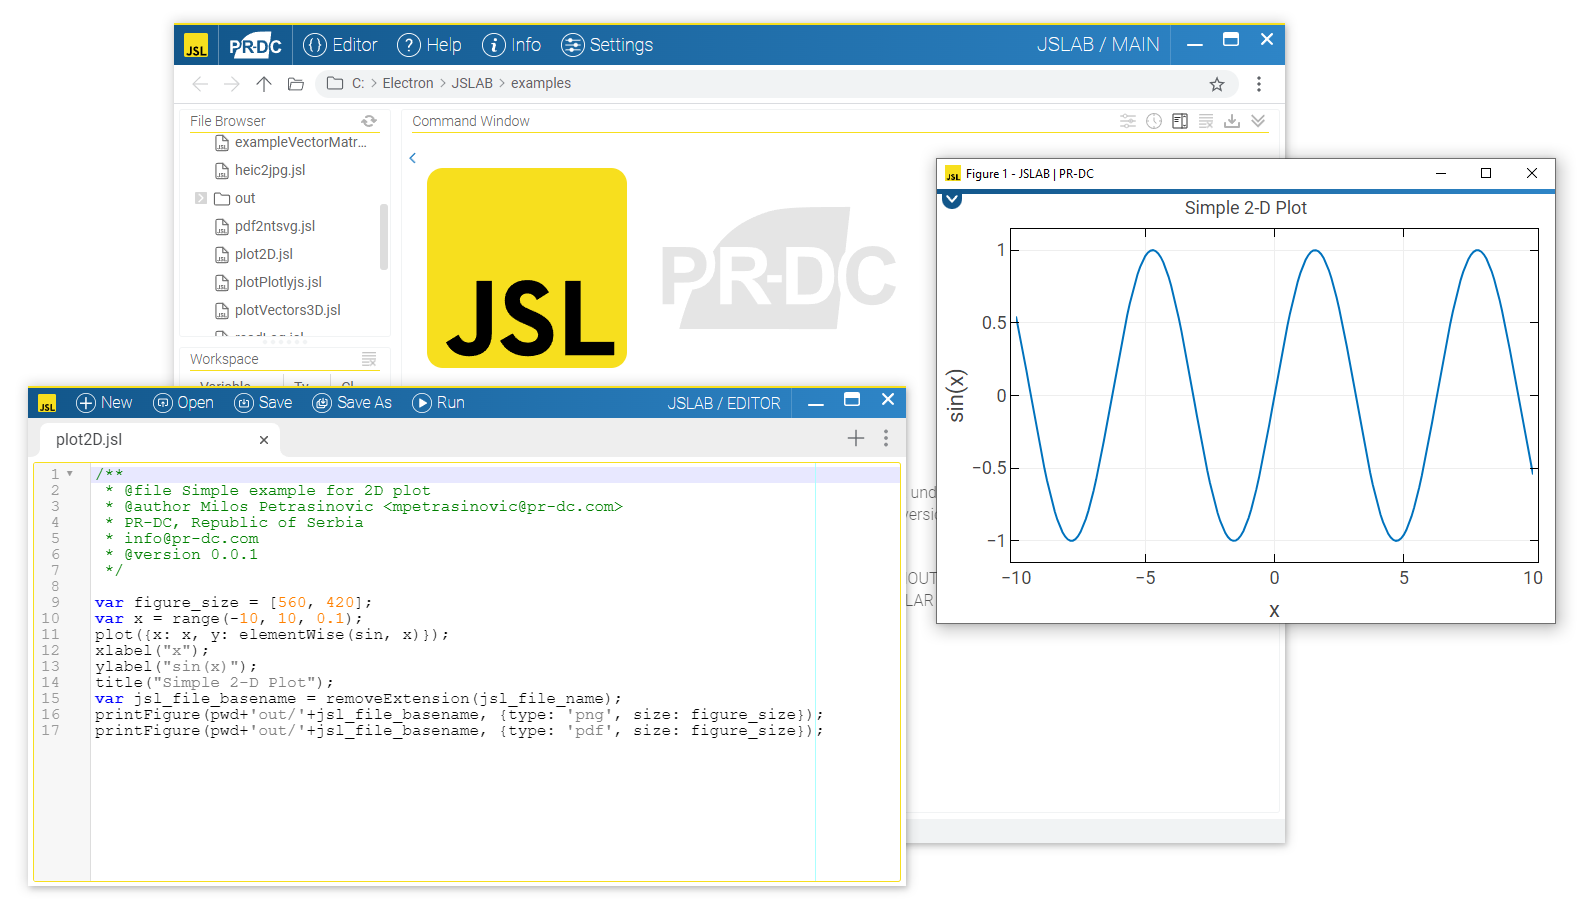
\includegraphics[width=0.8\textwidth]{resources/JSLAB_gui.png}
    \caption{JavaScript Laboratory (JSLAB) GUI}
    \label{fig:jslab}
\end{figure}

The program was developed to fulfill the need for performing calculations in a programming language that allows for code reuse in later project stages. JavaScript was chosen for its speed, dynamic nature, interpretability, extensive library support, large existing codebase, backing by major software companies, and the ability to create both desktop and mobile applications.

\textbf{JSLAB} offers a streamlined, dual-window interface designed to boost productivity and foster innovation. The main window combines a versatile workspace with a sandbox terminal, allowing users to run, test, and iterate on code in real time. The dedicated editor window introduces the \textbf{.JSL file format}—a plain text format tailored for \textbf{JSLAB} scripts. With advanced linting and intelligent autocompletion, the editor makes it easy to write precise, reusable code with minimal errors.

% ----------
\subsection{Why Choose JSLAB?}

\begin{itemize}
    \item \textbf{Backed by Leading Investments}

JavaScript is supported by major industry investments, ensuring continuous innovation and robust development. Our commitment to excellence makes \textbf{JSLAB} a trusted choice for professionals and organizations worldwide.

\item \textbf{Powered by JavaScript, Trusted by Giants}

Join the ranks of top companies who leverage JavaScript for their mission-critical applications. With \textbf{JSLAB}, you benefit from the same reliable and scalable technology that powers some of the most advanced projects on Earth and beyond.

\item \textbf{Thriving Community and Massive User Base}

Become part of a vibrant and growing community of JavaScript developter. Extensive support network and active forums ensure you always have the resources and assistance you need to succeed.

\item \textbf{Comprehensive Functionality Comparable to Leading Tools}

\textbf{JSLAB} bridges the gap between JavaScript and specialized scientific tools. Enjoy functionalities equivalent to MATLAB, GNU Octave, Python, R, and Julia, all within a single, unified platform. Perform data analysis, machine learning, numerical computations, and more with ease.

\item \textbf{Seamless and Native GUI with HTML, CSS, and SVG}

Design intuitive and visually appealing graphical user interfaces using native HTML, CSS, and SVG. Create interactive dashboards, custom visualizations, and responsive layouts without the need for additional frameworks.

\item \textbf{Extend with Native Modules via NPM and C++/C}

Enhance \textbf{JSLAB}’s capabilities by integrating native modules from npm, built with C++ and C. Tap into a vast ecosystem of extensions and customize your environment to meet your specific needs, ensuring maximum performance and flexibility.

\item \textbf{Join the JSLAB Revolution Today!}

Experience the seamless integration of powerful scientific computing and the flexibility of JavaScript. Whether you're developing complex algorithms, analyzing vast datasets, or creating innovative applications, \textbf{JSLAB} empowers you to achieve more.

\end{itemize}

% ----------
\subsection{License}
This program is free software: you can redistribute it and/or modify it under the terms of the GNU Lesser General Public License as published by the Free Software Foundation, either version 3 of the License, or (at your option) any later version.

This program is distributed in the hope that it will be useful, but WITHOUT ANY WARRANTY; without even the implied warranty of MERCHANTABILITY or FITNESS FOR A PARTICULAR PURPOSE. See the GNU Lesser General Public License for more details.

You should have received a copy of the GNU Lesser General Public License along with this program. If not, see \url{https://www.gnu.org/licenses/}.

\vspace{5mm}

Copyright (C) \yearvar\; PR-DC info@pr-dc.com

\vspace{8mm}

% --------------------
\section{About documentation}

This documentation serves as a comprehensive guide for both users and contributors of the \textbf{JSLAB} Library. It covers an introduction to the project, detailed features, installation and setup instructions, user interface overview, practical examples, coding standards, build instructions, contribution guidelines, and mechanisms for providing feedback.

The documentation is structured to provide clear and detailed information, ensuring that both new users and seasoned contributors can effectively utilize and contribute to the \textbf{JSLAB} project.

% --------------------
\section{Coding style}
\label{coding-style}

% ----------
\subsection{Documentation and Comments}

Clear documentation is essential for maintaining and understanding the codebase. We utilize JSDoc for structured documentation and inline comments to clarify complex logic.

\begin{itemize}
  \item \textbf{JSDoc:} Use JSDoc comments to document files, classes, methods, parameters, and return values.
  
  \item \textbf{Inline Comments:} Add comments to explain non-trivial code segments.
\end{itemize}

\begin{lstlisting}[style=JavaScriptStyle]
/**
* Constructs the JSLAB library environment.
* @param {Object} config Configuration options.
*/
constructor(config) {
  // Initialize properties
  this.config = config;
  // ... other initializations
}
\end{lstlisting}

% ----------
\subsection{Naming Conventions}
\begin{itemize}
  \item \textbf{Classes and Constants:} Use uppercase letters with underscores (e.g., \code{PRDC\_JSLAB\_LIB}).
  
  \item \textbf{Functions and Methods:} Use camelCase (e.g., \code{getFullFilePath}).
  
  \item \textbf{Variables:} Use lowercase letters with underscores (e.g., \code{new\_file\_path}).
  
  \item \textbf{Meaningful Names:} Choose self-explanatory names that convey the purpose clearly.
\end{itemize}

% ----------
\subsection{Code Structure and Modularization}
\begin{itemize}
  \item \textbf{Separation of Concerns:} Organize code into separate modules/files based on functionality.
  
  \item \textbf{Object-Oriented Design:} Use ES6 classes to encapsulate related properties and methods.
\end{itemize}

\begin{lstlisting}[style=JavaScriptStyle]
const { PRDC_JSLAB_EVAL } = require('./jslab-eval');

class PRDC_JSLAB_LIB {
  constructor(config) {
  this.eval = new PRDC_JSLAB_EVAL(this);
  // ... other initializations
  }
}
\end{lstlisting}

% ----------
\subsection{Error Handling}
\begin{itemize}
  \item \textbf{Try-Catch Blocks:} Use try-catch to handle potential errors gracefully.
  
  \item \textbf{Custom Errors:} Throw custom error objects for specific error scenarios.
\end{itemize}

\begin{lstlisting}[style=JavaScriptStyle]
try {
  return this.resolve(file_path);
} catch {
  this.jsl.env.error('Path resolution failed.');
}
\end{lstlisting}

% ----------
\subsection{State Management and Cleanup}
\begin{itemize}
  \item \textbf{Resource Tracking:} Maintain arrays and objects to track active asynchronous operations.
  
  \item \textbf{Cleanup Methods:} Implement methods to clear resources and reset the environment state.
\end{itemize}

% ----------
\subsection{Configuration Management}
\begin{itemize}
  \item \textbf{Centralized Configuration:} Use a dedicated class (\code{PRDC\_APP\_CONFIG}) to manage all configuration settings.
  
  \item \textbf{Conditional Configurations:} Adjust settings based on the runtime environment or command-line arguments.
\end{itemize}

% ----------
\subsection{Best Practices}
\begin{itemize}
  \item \textbf{Consistent Formatting:} Use a consistent code formatter to maintain uniform code style.
  
  \item \textbf{Meaningful Commit Messages:} Write clear and descriptive commit messages that explain the purpose of the changes.
  
  \item \textbf{Modular Code:} Write reusable and modular code to enhance maintainability and scalability.
  
  \item \textbf{Comprehensive Testing:} Implement thorough tests to ensure the reliability of your contributions.
\end{itemize}

% --------------------
\section{Installation}

You can install \textbf{JSLAB} by either downloading the latest stable release from GitHub or by building it from source. Choose the method that best fits your needs.

% ----------
\subsection{Download the Latest Stable Release}
\begin{itemize}
  \item Visit the JSLAB Releases Page on GitHub Repository: 
  
  \url{https://github.com/PR-DC/JSLAB/releases} 
  
  \item Download the appropriate installer and install program.

  \item Try examples from:

  \url{https://github.com/PR-DC/JSLAB/tree/master/examples}

\end{itemize}

% ----------
\subsection{Build from Source}

If you prefer to build \textbf{JSLAB} from source, follow the detailed \hyperref[build-instructions]{build instructions} available in this documentation.

% --------------------
\section{Build instructions}
\label{build-instructions}

% ----------
\subsection{Prerequisites}

In order to download necessary tools, clone the repository, and install dependencies via npm, you need network access.

\begin{itemize}
    \item \textbf{Node.js:} Ensure that Node.js is installed on your system. You can download it from the official website: 
    
    \url{https://nodejs.org/}
    
    \item \textbf{npm:} npm is typically installed alongside Node.js.
    
    \item \textbf{node-gyp:} node-gyp is installed alongside with application but it requires additional tools and libraries depending on your operating system. Follow the instructions for your specific OS from: 
    
    \url{https://github.com/nodejs/node-gyp}
    
    \item \textbf{Git:} Suggested for cloning the repository. Download it from the official website: 
    
    \url{https://git-scm.com/}

\end{itemize}

% ----------
\subsection{Installation Steps}
\begin{enumerate}
    \item Clone the JSLAB repository:
\begin{verbatim}
   git clone git clone https://github.com/PR-DC/JSLAB.git
\end{verbatim}
    
    \item Navigate to the project directory:
\begin{verbatim}
    cd JSLAB
\end{verbatim}

    \item Install the necessary dependencies:
\begin{verbatim}
    npm install
\end{verbatim}

    \item Start the application:
\begin{verbatim}
    npm start
\end{verbatim}

    \item Check examples from:

    \url{https://github.com/PR-DC/JSLAB/tree/master/examples}

\end{enumerate}

% --------------------
\section{Getting Started}

% ----------
\subsection{Main Window}
\label{sec:main-window}

The image below shows the main window of the \textbf{JSLAB} program.

\begin{figure}[H]
    \centering
    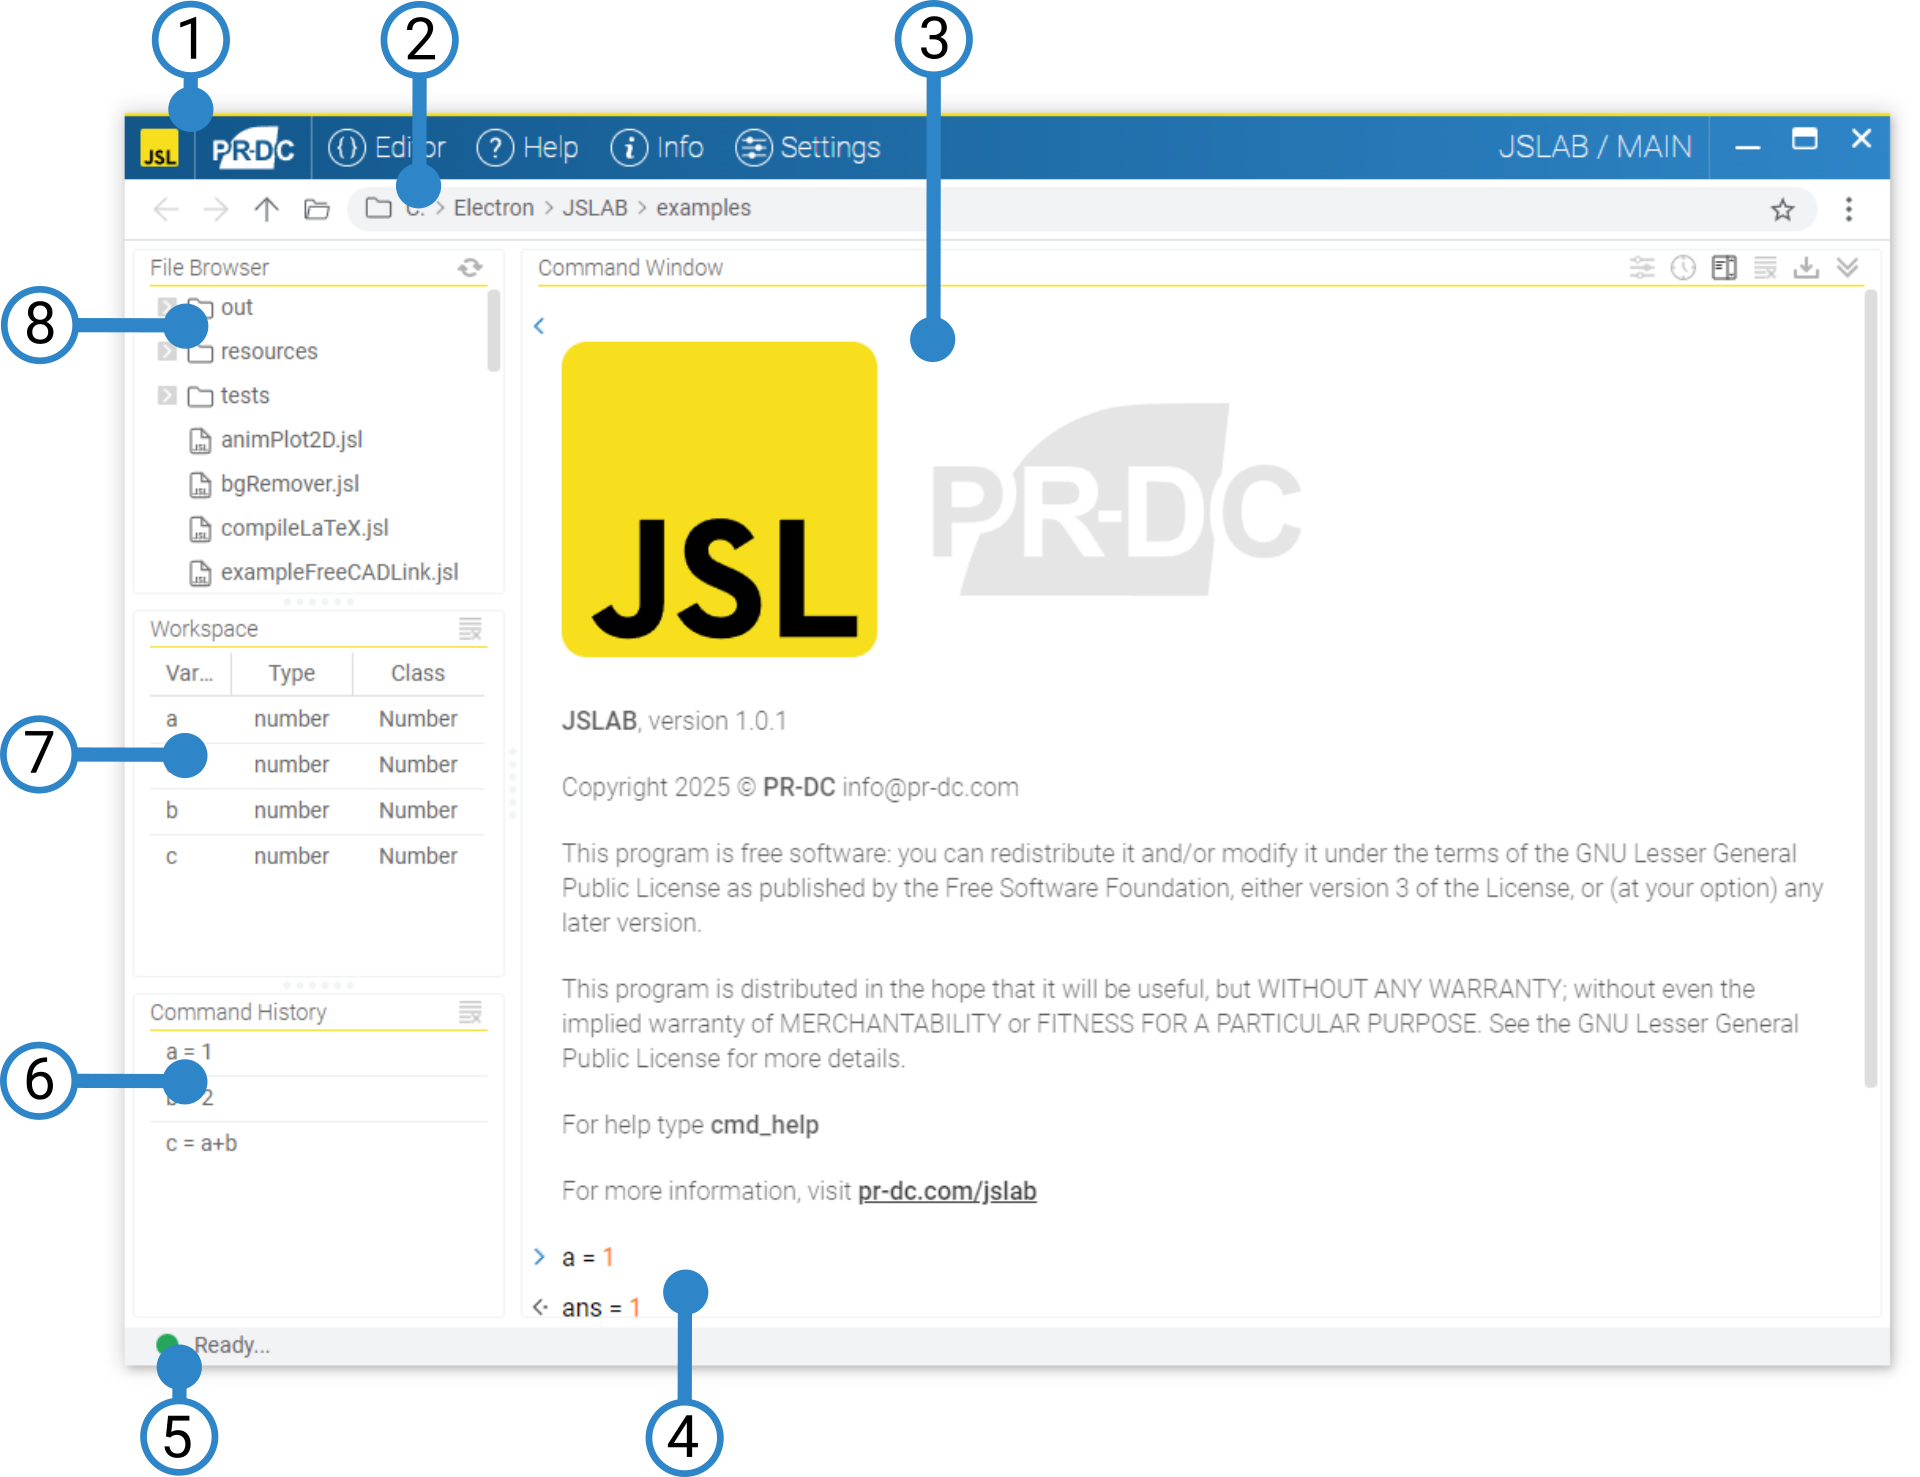
\includegraphics[width=0.8\textwidth]{resources/JSLAB_main_window.png}
    \caption{Main Window of JSLAB}
    \label{fig:main-window}
\end{figure}

Within the main window, there are various shortcuts defined in the help window---for example, the \texttt{[CTRL]} + \texttt{[H]} shortcut opens the help window.

In the image above, the following elements of the main window are numbered:
\begin{enumerate}
  \item \textbf{Main Window Header}\\
        A menu with options for opening the code editor window, viewing help, accessing program information, and opening the program settings (such as language settings; currently, Serbian in both Latin and Cyrillic scripts and English are available).
  \item \textbf{Workspace Navigation}\\
        Icons for navigating through folders and opening a folder selection window. Besides the current workspace folder, you can save additional paths that will be used when running scripts.
  \item \textbf{Command Window}\\
        Located in the central right panel, this window displays messages from the workspace after code execution.
  \item \textbf{Command Input Field}\\
        Located at the bottom of the central right panel, this field is used to send commands to the workspace. As you type, suggestions for completing the command automatically appear based on the currently active workspace. You can also navigate through the history of entered commands. After typing a command and pressing \texttt{[ENTER]}, the command is executed in the workspace.
  \item \textbf{Status Bar}\\
        A bar at the bottom of the window displaying the current state of the workspace. In the bottom left corner, an icon changes color based on that state; clicking the icon displays a tooltip with information about what is currently active in the workspace.
  \item \textbf{Command History}\\
        Located in the lower part of the left central panel, this section allows you to track the sequence of executed commands and easily re-execute a command (by double-clicking on it).
  \item \textbf{Workspace Variables}\\
        In the central part of the left panel, this area displays the name, type, and class of each active global variable created by the user in the workspace.
  \item \textbf{File Browser}\\
        Located in the upper part of the left panel, this area shows folders and files, which can be directly opened within the editor.
\end{enumerate}

\begin{quotation}
\textbf{Note:} The command window is ideal for entering a few commands. However, for more complex tasks, scripts are used.
\end{quotation}


% ----------
\subsection{Editor Window}
\label{sec:editor-window}

For \textbf{JSLAB} scripts, the \texttt{.jsl} extension is used to distinguish them from the standard \texttt{.js} extension for JavaScript. Scripts are executed by providing the script path as the sole argument to the \texttt{run} function. For writing or editing code in a script, it is best to use the built-in code editor (which can be opened with the \texttt{editor} command or the \texttt{edit()} function). The code editor window is shown in the image below.

\begin{figure}[H]
    \centering
    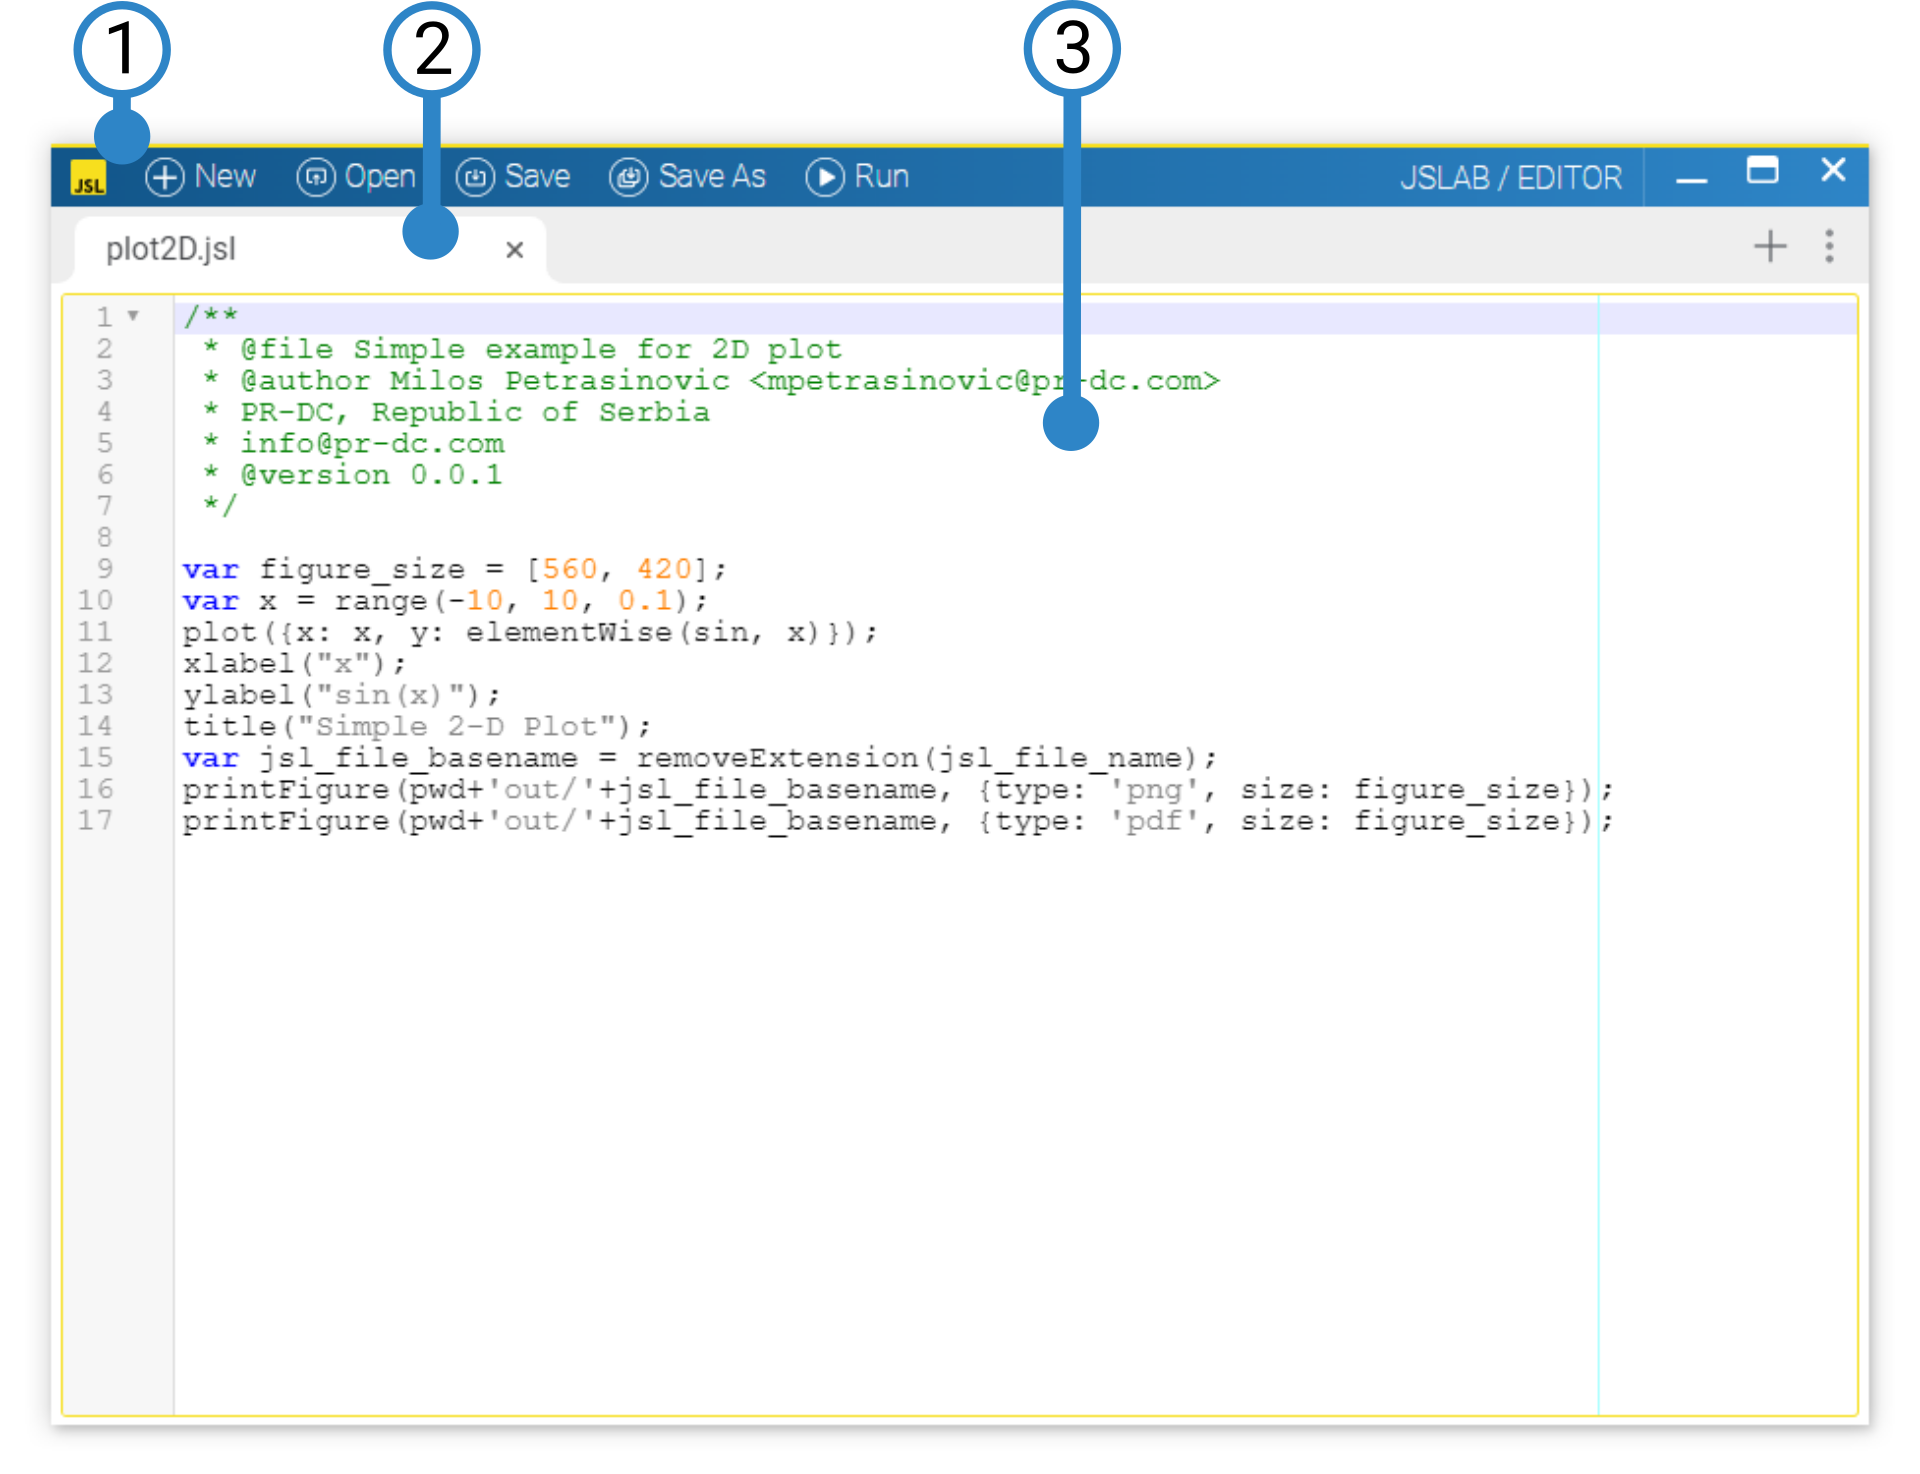
\includegraphics[width=0.8\textwidth]{resources/JSLAB_editor_window.png}
    \caption{Editor Window of JSLAB}
    \label{fig:editor-window}
\end{figure}

In the image above, the following elements of the code editor window are numbered:
\begin{enumerate}
  \item \textbf{Editor Window Header}\\
        At the very top of the window, there is a menu with options for creating new scripts, opening existing ones, saving open scripts, and directly executing scripts in the workspace.
  \item \textbf{Script Tabs}\\
        Located just below the header, these tabs allow you to switch between the active scripts being edited and to open or close scripts.
  \item \textbf{Script Text Editor}\\
        This is the area where the script code is displayed. As you type, suggestions for completing commands automatically appear based on the currently active workspace---similar to the command window. This text editor provides many advanced features for working with code, including syntax checking, suggestions, the ability to collapse certain code blocks, and highlighting of the current active line.
\end{enumerate}

The editor also includes additional advanced features for code input, such as searching through the code and performing text replacements (the search popup can be opened by pressing \texttt{[CTRL]} + \texttt{[F]}).

Most importantly, code can be executed in two ways:
\begin{itemize}
  \item By entering commands in the command input field of the command window.
  \item By running a script using the \code{run()} function or directly from the editor window.
\end{itemize}


% ----------
\subsection{Programming}
\label{sec:programming}

Programming in \textbf{JSLAB} is based on the full feature set of \textbf{JavaScript} and \textbf{Node.js}, combined with \textbf{HTML} and \textbf{CSS} for building graphical user interfaces (GUI). The application also provides a range of \textbf{built-in functions} that simplify certain tasks---like plotting with the \code{plot()} function. All implemented functions and classes are documented for easy reference.

\subsubsection{Accessing Documentation}
Multiple approaches are available to view documentation directly from \textbf{JSLAB}:
\begin{itemize}
  \item \textbf{Built-in help functions:} \code{help()}, \code{doc()}, \code{documentation()}, \code{helpSearch()}, \code{docSearch()}, \code{documentationSearch()}
  \item \textbf{HTML documentation:} Openable via the \code{openDoc()} or \code{openDocumentation()} functions
  \item \textbf{Function source code:} See the implementation of a built-in function with \code{source("functionName")} (e.g., \code{source("plot")})
\end{itemize}

\subsubsection{Working with Scripts and Examples}
\textbf{JSLAB} scripts typically use a \texttt{.jsl} extension to distinguish them from standard \texttt{.js} files. You can run scripts from the command window with \code{run("scriptPath")}, or open them in the built-in editor (using the \code{editor} command or the \code{edit("scriptName.jsl")} function).

For bundled example scripts:
\begin{itemize}
  \item \textbf{List examples:} \code{getExamples()}
  \item \textbf{Open a specific example:} \code{openExample("exampleName")}
  \item \textbf{Open the examples folder:} \code{openExamplesFolder()}
  \item \textbf{Navigate to the examples folder:} \code{goToExamplesFolder()}
\end{itemize}

\subsubsection{Resetting the Environment}
\begin{itemize}
  \item \textbf{Reset workspace (sandbox):} \code{resetSandbox()} clears current workspace variables.
  \item \textbf{Reset the entire application:} \code{resetApp()} returns the application to its initial state.
\end{itemize}

\subsubsection{Advanced Chromium Tools}
Since \textbf{JSLAB} is built on \textbf{Chromium}, you can leverage its powerful developer tools for debugging and performance analysis:
\begin{itemize}
  \item \code{openDevTools()}: Open Developer Tools
  \item \code{openWindowDevTools()}: Open Window Developer Tools
\end{itemize}

The \textbf{Performance} tab in the developer tools is particularly useful for optimizing your scripts, helping to identify potential slow-downs and bottlenecks.

% --------------------
\section{Examples}

% ----------
\subsection{Animated 2D Plot}
\label{sec:animated-2d-plot}

A 2D plot animation like this is essential for visualizing real-time data changes, enabling dynamic tracking of evolving values and providing immediate insight into trends or fluctuations as they happen.

\begin{figure}[H]
    \centering
    % If you experience issues with GIFs, consider converting to a supported format.
    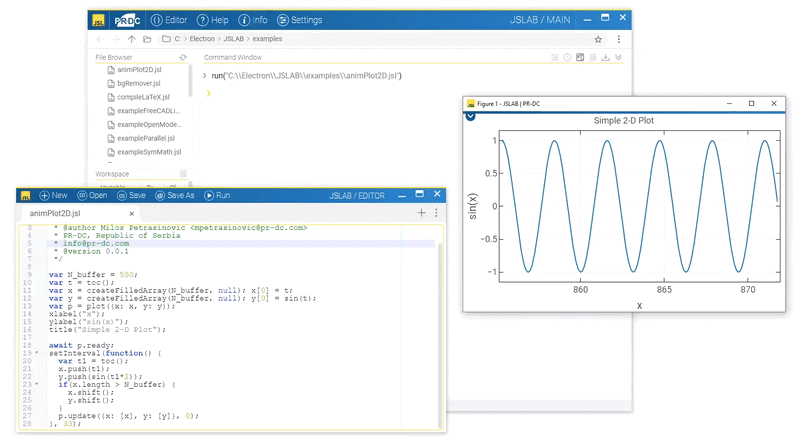
\includegraphics[width=0.8\textwidth]{resources/JSLAB_2D_plot.png}
    \caption{Animated 2D Plot}
    \label{fig:animated-2d-plot}
\end{figure}

\begin{lstlisting}[style=JavaScriptStyle]
// JavaScript Example
var N_buffer = 500;
var t = toc();
var x = createFilledArray(N_buffer, null); x[0] = t;
var y = createFilledArray(N_buffer, null); y[0] = sin(t);
var p = plot({x: x, y: y});
xlabel("x");
ylabel("sin(x)");
title("Simple 2-D Plot");

await p.ready;
setInterval(function() {
  var t1 = toc();
  x.push(t1);
  y.push(sin(t1*2));
  if(x.length > N_buffer) {
    x.shift();
    y.shift();
  }
  p.update({x: [x], y: [y]}, 0);
}, 33);
\end{lstlisting}

% ----------
\subsection{3D Plot with Vectors}
\label{sec:3d-plot-vectors}

3D plots are essential for illustrating spatial relationships and complex vector interactions, allowing for a deeper understanding of data across three dimensions.

\begin{figure}[H]
    \centering
    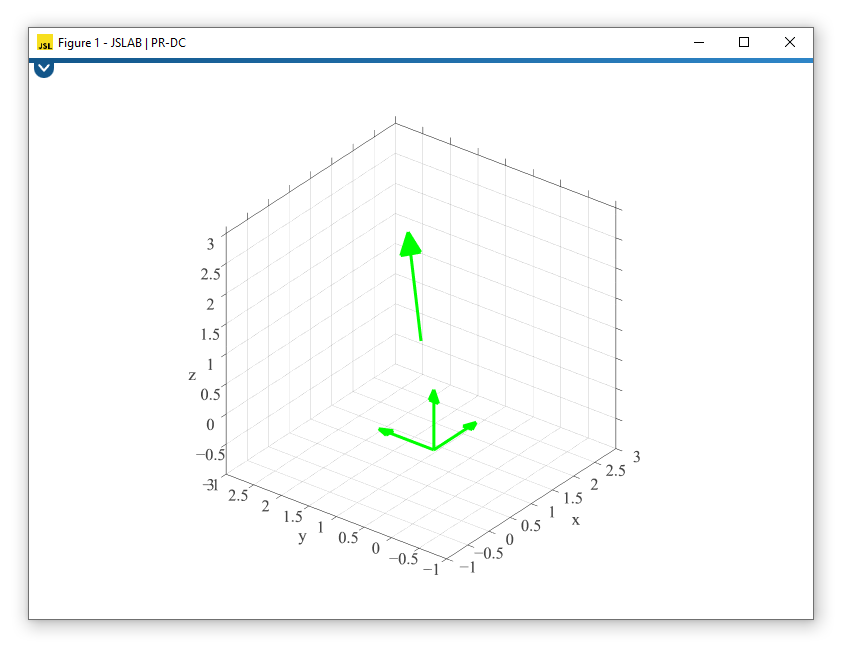
\includegraphics[width=0.8\textwidth]{resources/JSLAB_3D_plot.png}
    \caption{3D Plot with Vectors}
    \label{fig:3d-plot-vectors}
\end{figure}

\begin{lstlisting}[style=JavaScriptStyle]
// JavaScript Example
var x = [0, 0, 0, 1, 0];
var y = [0, 0, 0, 1, 0];
var z = [0, 0, 0, 1, 0];

var u = [1, 0, 0, 1, -1];
var v = [0, 1, 0, 1, 0];
var w = [0, 0, 1, 1, 0];

var head_scale = 0.2;
var head_angleFactor = 0.4;

var vectors = createVectors3D(x, y, z, u, v, w, head_scale, head_angleFactor, {color: "#0f0", width: 6});

figure(1);
plot([
  vectors.line, vectors.head
], {'showLegend': false, 'font': {family: 'LatinModern', size: 14}});
xlabel("x");
ylabel("y");
zlabel("z");
xlim([-1, 3]);
ylim([-1, 3]);
zlim([-1, 3]);
\end{lstlisting}

% ----------
\subsection{3D Graphics}
\label{sec:3d-graphics}

3D graphics are vital for creating immersive visualizations that bring complex structures and spatial relationships to life, enabling a more intuitive understanding and interaction with digital models in fields like simulation, design, and data analysis.

\begin{figure}[H]
    \centering
    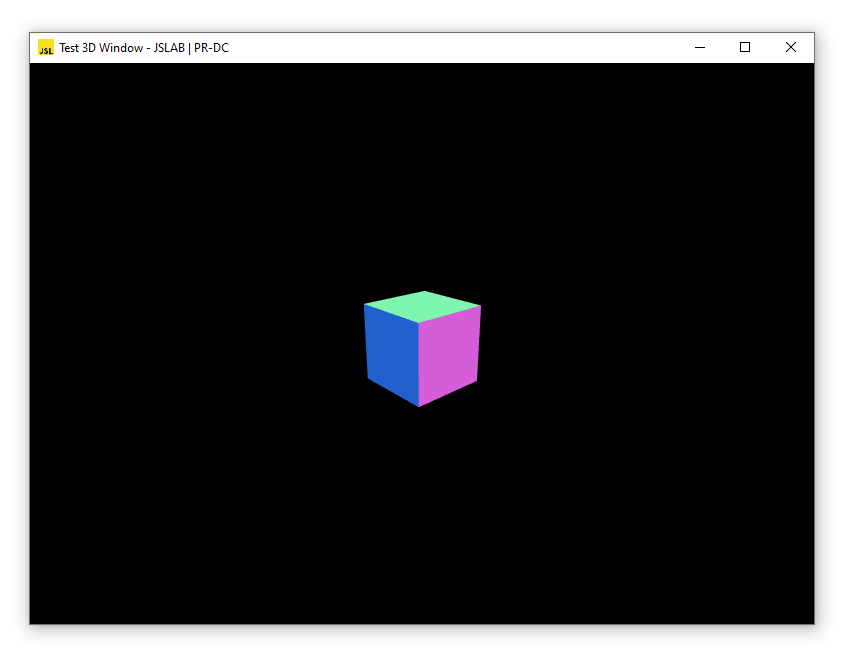
\includegraphics[width=0.8\textwidth]{resources/JSLAB_3D_graphics.png}
    \caption{3D Graphics Example}
    \label{fig:3d-graphics}
\end{figure}

\begin{lstlisting}[style=JavaScriptStyle]
// JavaScript Example
var win = await openWindow3D();
win.document.title = "Test 3D Window - JSLAB | PR-DC";
var THREE = win.THREE;

const width = win.innerWidth, height = win.innerHeight;

// init
const camera = new THREE.PerspectiveCamera( 70, width / height, 0.01, 10 );
camera.position.z = 1;

const scene = new THREE.Scene();

const geometry = new THREE.BoxGeometry( 0.2, 0.2, 0.2 );
const material = new THREE.MeshNormalMaterial();

const mesh = new THREE.Mesh( geometry, material );
scene.add( mesh );

const renderer = new THREE.WebGLRenderer( { antialias: true } );
renderer.setSize( width, height );
renderer.setAnimationLoop( animate );
win.document.body.appendChild( renderer.domElement );

// Handle window resizing
window.addEventListener('resize', onWindowResize, false);

function onWindowResize() {
  camera.aspect = win.innerWidth / win.innerHeight;
  camera.updateProjectionMatrix();
  renderer.setSize(win.innerWidth, win.innerHeight);
}

function animate( time ) {
  mesh.rotation.x = time / 2000;
  mesh.rotation.y = time / 1000;
  
  renderer.render( scene, camera );
}
\end{lstlisting}

% ----------
\subsection{Parallel Execution}
\label{sec:parallel-execution}

Parallel execution is critical for handling computationally intensive tasks, as it allows multiple operations to run simultaneously, significantly reducing processing time and improving efficiency by utilizing all available CPU cores.

\begin{lstlisting}[style=JavaScriptStyle]
// JavaScript Example
var computeSquare = (i) => i * i;

// Run parallel exectuion 
var results = await parallel.parfor(0, 20, 1, 
  parallel.getProcessorsNum(), {}, undefined, computeSquare);
disp(results);
\end{lstlisting}

% ----------
\subsection{Vector and Matrix Operations}
\label{sec:vector-matrix}

Vector and matrix operations are fundamental for efficiently performing complex mathematical computations in fields like physics, engineering, and computer graphics, enabling quick transformations, optimizations, and solutions in multidimensional spaces.

\begin{lstlisting}[style=JavaScriptStyle]
// JavaScript Example
var v1 = vec.new(1, 2, 3);
var v2 = vec.new([4, 8, 6]);
const v_cross = v1.cross(v2);

var A = mat.new([
    [1, 2],
    [3, 4]
]);
const b = mat.new([
    [5],
    [11]
]);
const x = A.linsolve(b);
disp('Solution to linear system A * x = b:');
disp(x);
\end{lstlisting}

% ----------
\subsection{Symbolic Math}
\label{sec:symbolic-math}

Symbolic math computations are essential for achieving high precision in mathematical modeling, automating algebraic simplifications, and enabling dynamic formula manipulation, which enhances the accuracy and functionality of tools in scientific, engineering, and educational software.

\begin{figure}[H]
    \centering
    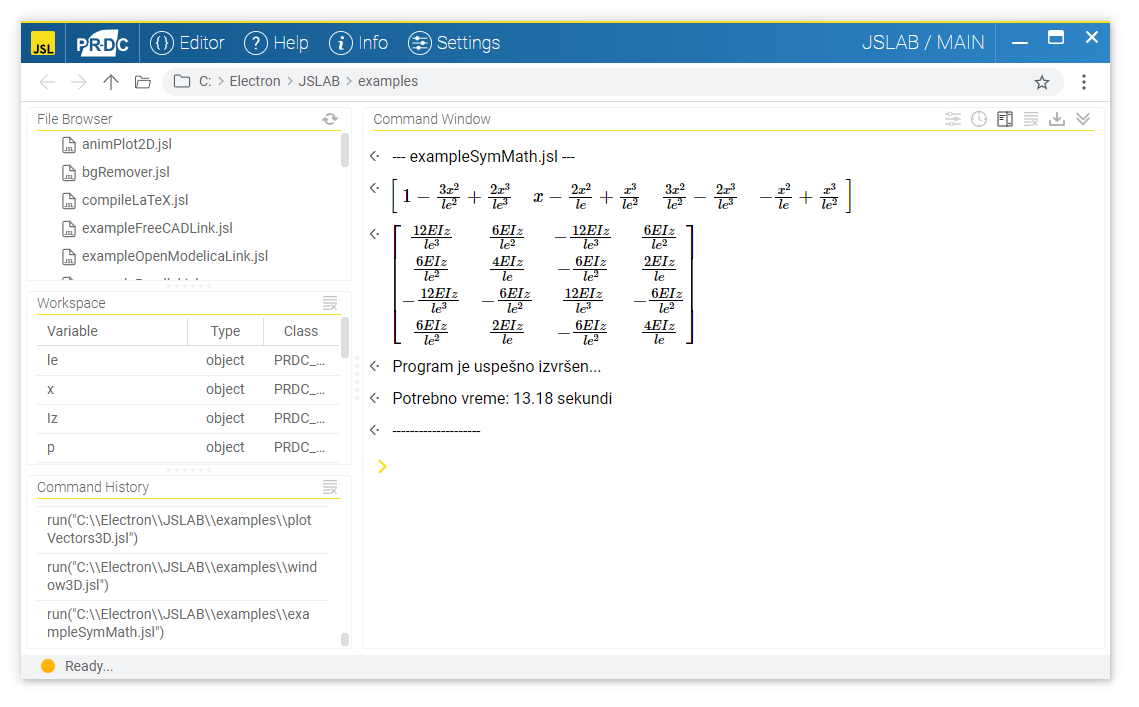
\includegraphics[width=0.8\textwidth]{resources/JSLAB_symbolic.png}
    \caption{Symbolic Math Example}
    \label{fig:symbolic-math}
\end{figure}

\begin{lstlisting}[style=JavaScriptStyle]
// JavaScript Example
var le, x, E, Iz;
var p, P, invP, N, d2N;
var k_int, k_e_stretching, k_e_torsion;
var xi = range(0, 1, 0.01);

await sym.load();
[le, x, E, Iz] = sym.syms(['le', 'x', 'E', 'Iz']);

P = sym.mat([
  [1, 0, 0, 0], 
  [0, 1, 0, 0], 
  [1, le, sym.pow(le, 2), sym.pow(le, 3)], 
  [0, 1, sym.mul(2, le), sym.mul(3, sym.pow(le, 2))]
]);
p = sym.mat([[1, x, sym.pow(x, 2), sym.pow(x, 3)]]);

invP = sym.inv(P);
N = sym.mul(p, invP);
d2N = sym.diff(N, 'x', 2);

k_int = sym.mul(E, Iz, sym.intg(sym.mul(sym.transp(d2N), d2N), x, [0, le]));

Ni = sym.subs(sym.subs(N, le, 1), x, xi).toNumeric();
var N_flat = Ni.flat();

sym.showLatex(N);
sym.showLatex(k_int);
\end{lstlisting}

% ----------
\subsection{FreeCAD Link}
\label{sec:freecad-link}

Integration with FreeCAD is essential for enabling automated, precise 3D modeling workflows within applications, allowing complex geometries, structures, and engineering designs to be generated, modified, and visualized programmatically, which significantly enhances productivity in design and simulation processes.

\begin{figure}[H]
    \centering
    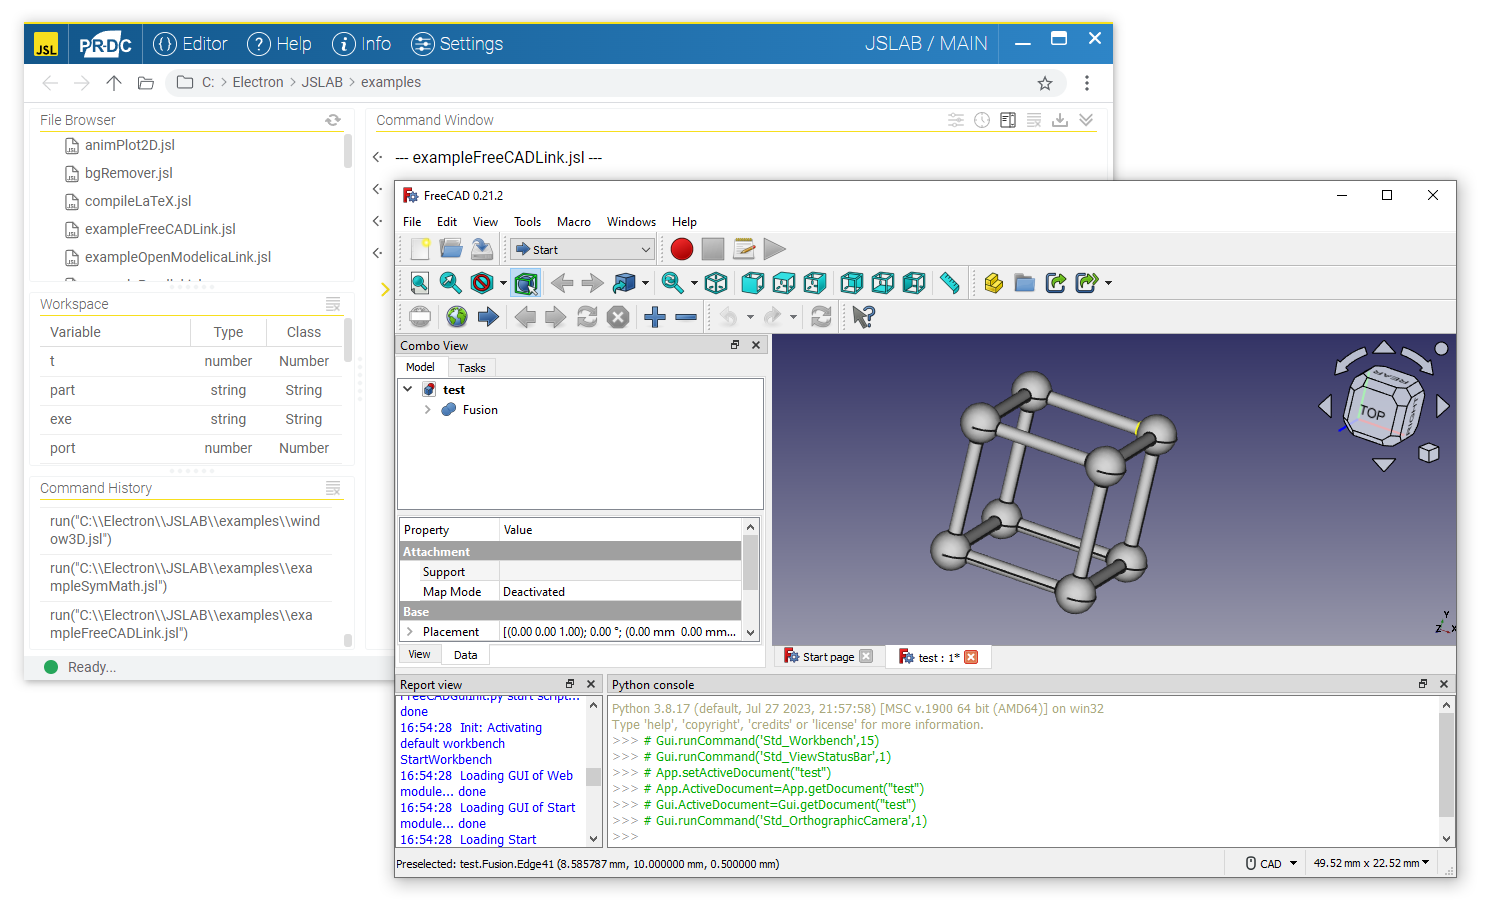
\includegraphics[width=0.8\textwidth]{resources/JSLAB_FreeCADLink.png}
    \caption{FreeCAD Link Example}
    \label{fig:freecad-link}
\end{figure}

\begin{lstlisting}[style=JavaScriptStyle]
// JavaScript Example
var nodes = [
  [0, 0, 0],
  [0, 10, 0],
  [10, 10, 0],
  [10, 0, 0],
  [0, 0, 10],
  [0, 10, 10],
  [10, 10, 10],
  [10, 0, 10]
];
var D = createFilledArray(nodes.length, 3);

var lines = [];
for(var i = 0; i < 4; i++) {
  var j = i+1;
  if(i == 3) {
    j = 0;
  }
  lines.push([...nodes[i], ...nodes[j]]);
  lines.push([...nodes[i+4], ...nodes[j+4]]);
  lines.push([...nodes[i], ...nodes[i+4]]);
}
var d = createFilledArray(lines.length, 1);

// Generate JSON
var nodesFile = pwd + 'out/nodes.json';
var data = {
  'Coordinates': nodes,
  'Diameters': D
};
writeFile(nodesFile, stringify(data));
var data = {
  'Coordinates': lines,
  'Diameters': d
};
beamsFile = pwd + 'out/beams.json';
writeFile(beamsFile, stringify(data));

// Run FreeCADLink 
await freecad_link.start(exe, {
  port: port,
  host: host,
  timeout: timeout,
  startup_timeout: startup_timeout
}); // Start FreeCAD program

await freecad_link.newDocument(part);
await freecad_link.callScript('MakeNodes', nodesFile, timeout);
await freecad_link.callScript('MakeBeams', beamsFile, timeout);
await freecad_link.callScript('MakeFusion', [], timeout);
await freecad_link.saveAs(model, timeout);
//await freecad_link.quit(); // Close program

deleteFile(nodesFile);
deleteFile(beamsFile);
\end{lstlisting}

% ----------
\subsection{OpenModelica Link}
\label{sec:openmodelica-link}

Integration with OpenModelica is crucial for enabling advanced simulation and analysis of complex dynamic systems directly within applications, allowing engineers to model, test, and optimize system behavior seamlessly, which enhances efficiency in design and validation processes.

\begin{lstlisting}[style=JavaScriptStyle]
// JavaScript Example
await om_link.start(exe); // Start OpenModelica program
disp(await om_link.sendExpression('getVersion()'));

disp(await om_link.sendExpression("model a end a;"));
disp(await om_link.sendExpression('loadFile("'+model+'")'));
disp(await om_link.sendExpression("getClassNames()"));
disp(await om_link.sendExpression("simulate(BouncingBall)"));
await om_link.close();
\end{lstlisting}

% --------------------
\section{Contributing}

% ----------
\subsection{Setting Up the Development Environment}

Follow the detailed \hyperref[build-instructions]{build instructions} available in this documentation.

% ----------
\subsection{Making Changes}

Follow the \hyperref[coding-style]{coding style and best practices} available in this documentation.

% ----------
\subsection{Submitting Changes}

\begin{enumerate}
    \item Create a new branch for your feature or bugfix:
\begin{verbatim}
    git checkout -b feature/your-feature-name
\end{verbatim}

    \item Make your changes and commit them with clear messages:
\begin{verbatim}
   git commit -m "Add feature X to improve Y"
\end{verbatim}

    \item Push your branch to your forked repository:
\begin{verbatim}
    git push origin feature/your-feature-name
\end{verbatim}

    \item Submit a Pull Request (PR) detailing your changes.
\end{enumerate}

% ----------
\subsection{Testing}
Before submitting a PR, ensure that all tests pass and add new tests for any new functionality you introduce.

% ----------
\subsection{Reviewing Process}
All PRs are subject to review by the maintainers. Be prepared to make revisions based on feedback to align with project standards.

% ----------
\subsection{Best Practices}

\begin{itemize}
    \item \textbf{Consistent Formatting:} Use a consistent code formatter (e.g., Prettier) to maintain uniform code style.

    \item \textbf{Meaningful Commit Messages:} Write clear and descriptive commit messages that explain the purpose of the changes.

    \item \textbf{Modular Code:} Write reusable and modular code to enhance maintainability and scalability.

    \item \textbf{Comprehensive Testing:} Implement thorough tests to ensure the reliability of your contributions.
\end{itemize}

% --------------------
\section{Feedback}

Your feedback is invaluable in improving the \textbf{JSLAB} application. Whether you encounter bugs, have feature requests, or need assistance, please reach out through the following channels:

\begin{itemize}
    \item \textbf{GitHub Issues:} Report bugs or suggest features by opening an issue in the GitHub repository.
    
    \item \textbf{Email}: Contact us directly at \href{mailto:info@pr-dc.com}{info@pr-dc.com} or main author at \href{mailto:mpetrasinovic@pr-dc.com}{mpetrasinovic@pr-dc.com}.
\end{itemize}

We encourage active participation and appreciate all forms of feedback that help us enhance the functionality and usability of \textbf{JSLAB}.

% --------------------
\section{Code references}

\subsection{basic}
\vspace{5mm}
\noindent \code{\texttt{ans}}{\color{jsl-gray}\vspace{2mm}\hrule}\vspace{4mm}


\noindent \textbf{Type:} \texttt{<Unknown>}

\noindent Stores the result of the last evaluated expression.

\vspace{5mm}
\noindent \codeBlock{\texttt{clear()}}{\color{jsl-gray}\vspace{2mm}\hrule\vspace{4mm}}


\noindent Clears all defined variables in the current context.

\vspace{5mm}
\noindent \codeBlock{\texttt{clc()}}{\color{jsl-gray}\vspace{2mm}\hrule\vspace{4mm}}


\noindent Clears the console screen.

\vspace{5mm}
\noindent \codeBlock{\texttt{cls()}}{\color{jsl-gray}\vspace{2mm}\hrule\vspace{4mm}}


\noindent Clears the console screen. Alias for \textasciigrave{}clc\textasciigrave{}.

\vspace{5mm}
\noindent \code{\texttt{version}}{\color{jsl-gray}\vspace{2mm}\hrule}\vspace{4mm}


\noindent \textbf{Type:} \texttt{<Unknown>}

\noindent Returns the current version of the JSLAB.

\vspace{5mm}
\noindent \code{\texttt{platform}}{\color{jsl-gray}\vspace{2mm}\hrule}\vspace{4mm}


\noindent \textbf{Type:} \texttt{<Unknown>}

\noindent Returns the platform on which JSLAB is running.

\vspace{5mm}
\noindent \code{\texttt{jsl\_file\_name}}{\color{jsl-gray}\vspace{2mm}\hrule}\vspace{4mm}


\noindent \textbf{Type:} \texttt{<Unknown>}

\noindent Returns the file name of the current JSLAB script.

\vspace{5mm}
\noindent \codeBlock{\texttt{info()}}{\color{jsl-gray}\vspace{2mm}\hrule\vspace{4mm}}


\noindent Provides information about the current environment.

\vspace{5mm}
\noindent \codeBlock{\texttt{settings()}}{\color{jsl-gray}\vspace{2mm}\hrule\vspace{4mm}}


\noindent Accesses or modifies the user settings for JSLAB.

\vspace{5mm}
\noindent \codeBlock{\texttt{cmd\_help()}}{\color{jsl-gray}\vspace{2mm}\hrule\vspace{4mm}}


\noindent Provides help information for JSLAB commands.

\vspace{5mm}
\noindent \codeBlock{\texttt{editor()}}{\color{jsl-gray}\vspace{2mm}\hrule\vspace{4mm}}


\noindent Accesses the code editor interface within JSLAB.

\vspace{5mm}
\noindent \code{\texttt{pwd}}{\color{jsl-gray}\vspace{2mm}\hrule}\vspace{4mm}


\noindent \textbf{Type:} \texttt{<Unknown>}

\noindent Returns the current working directory.

\vspace{5mm}
\noindent \codeBlock{\texttt{breakpoint()}}{\color{jsl-gray}\vspace{2mm}\hrule\vspace{4mm}}


\noindent Sets a breakpoint in the code for debugging.

\vspace{5mm}
\noindent \code{\texttt{debug\_flag}}{\color{jsl-gray}\vspace{2mm}\hrule}\vspace{4mm}


\noindent \textbf{Type:} \texttt{<Unknown>}

\noindent Returns the current debug flag status.

\vspace{5mm}
\noindent \code{\texttt{debug}}{\color{jsl-gray}\vspace{2mm}\hrule}\vspace{4mm}


\noindent \textbf{Type:} \texttt{<Unknown>}

\noindent Enables or disables debug mode.

\vspace{5mm}
\noindent \codeBlock{\texttt{pause()}}{\color{jsl-gray}\vspace{2mm}\hrule\vspace{4mm}}


\noindent Pauses the execution of the current script.

\vspace{5mm}
\noindent \codeBlock{\texttt{stoppoint()}}{\color{jsl-gray}\vspace{2mm}\hrule\vspace{4mm}}


\noindent Sets a stop point in the script execution.

\vspace{5mm}
\noindent \codeBlock{\texttt{logpoint()}}{\color{jsl-gray}\vspace{2mm}\hrule\vspace{4mm}}


\noindent Sets a log point to record information during execution.

\vspace{5mm}
\noindent \codeBlock{\texttt{updatepoint()}}{\color{jsl-gray}\vspace{2mm}\hrule\vspace{4mm}}


\noindent Updates specific points in the script during execution.

\vspace{5mm}
\noindent \codeBlock{\texttt{checkStop()}}{\color{jsl-gray}\vspace{2mm}\hrule\vspace{4mm}}


\noindent Checks if the execution should stop based on conditions.

\vspace{5mm}
\noindent \codeBlock{\texttt{endPoint()}}{\color{jsl-gray}\vspace{2mm}\hrule\vspace{4mm}}


\noindent Marks the endpoint of a script or process.

\vspace{5mm}
\noindent \codeBlock{\texttt{run(script\_path, lines, [silent], [force\_run])}}{\color{jsl-gray}\vspace{2mm}\hrule\vspace{4mm}}


\noindent \textbf{Parameters:}
\begin{itemize}
  \item \texttt{script\_path} \texttt{<string>}: The path to the script to run.
  \item \texttt{lines} \texttt{<Array.<number>>}: An array of line numbers to run or focus on within the script.
  \item \texttt{silent} \texttt{<boolean>}: Whether to suppress output from the script execution.
  \item \texttt{force\_run} \texttt{<Boolean>}: If true, forces the script to run even if stop conditions are met.
\end{itemize}

\noindent Runs a script from a specified path, optionally focusing on specific lines and controlling output visibility.

\vspace{5mm}
\noindent \codeBlock{\texttt{helpToJSON([name], [type])}}{\color{jsl-gray}\vspace{2mm}\hrule\vspace{4mm}}


\noindent \textbf{Parameters:}
\begin{itemize}
  \item \texttt{name} \texttt{<string>}: The name of the documentation item.
  \item \texttt{type} \texttt{<string>}: The type of the documentation (e.g., 'category').
\end{itemize}

\noindent \textbf{Returns:} \texttt{<string>}: The JSON string of the documentation or undefined if not found.

\noindent Retrieves documentation in JSON format based on the provided name and type.

\vspace{5mm}
\noindent \codeBlock{\texttt{help(name, type)}}{\color{jsl-gray}\vspace{2mm}\hrule\vspace{4mm}}


\noindent \textbf{Parameters:}
\begin{itemize}
  \item \texttt{name} \texttt{<string>}: The name of the documentation item.
  \item \texttt{type} \texttt{<string>}: The type of the documentation.
\end{itemize}

\noindent \textbf{Returns:} \texttt{<string>}: The JSON string of the documentation or undefined if not found.

\noindent Retrieves documentation based on the provided name and type.

\vspace{5mm}
\noindent \codeBlock{\texttt{doc(name, type)}}{\color{jsl-gray}\vspace{2mm}\hrule\vspace{4mm}}


\noindent \textbf{Parameters:}
\begin{itemize}
  \item \texttt{name} \texttt{<string>}: The name of the documentation item.
  \item \texttt{type} \texttt{<string>}: The type of the documentation.
\end{itemize}

\noindent \textbf{Returns:} \texttt{<string>}: The JSON string of the documentation or undefined if not found.

\noindent Retrieves documentation based on the provided name and type.

\vspace{5mm}
\noindent \codeBlock{\texttt{documentation(name, type)}}{\color{jsl-gray}\vspace{2mm}\hrule\vspace{4mm}}


\noindent \textbf{Parameters:}
\begin{itemize}
  \item \texttt{name} \texttt{<string>}: The name of the documentation item.
  \item \texttt{type} \texttt{<string>}: The type of the documentation.
\end{itemize}

\noindent \textbf{Returns:} \texttt{<string>}: The JSON string of the documentation or undefined if not found.

\noindent Retrieves documentation based on the provided name and type.

\vspace{5mm}
\noindent \codeBlock{\texttt{helpSearch(query)}}{\color{jsl-gray}\vspace{2mm}\hrule\vspace{4mm}}


\noindent \textbf{Parameters:}
\begin{itemize}
  \item \texttt{query} \texttt{<string>}: The search query containing keywords to match within the documentation.
\end{itemize}

\noindent \textbf{Returns:} \texttt{<Array.<Object>>}: Array of matching documentation entries, each entry containing \textasciigrave{}type\textasciigrave{} and \textasciigrave{}category\textasciigrave{} properties.

\noindent Searches the documentation for methods that match all words in the given query, regardless of order.

\vspace{5mm}
\noindent \codeBlock{\texttt{docSearch(query)}}{\color{jsl-gray}\vspace{2mm}\hrule\vspace{4mm}}


\noindent \textbf{Parameters:}
\begin{itemize}
  \item \texttt{query} \texttt{<string>}: The search query containing keywords to match within the documentation.
\end{itemize}

\noindent \textbf{Returns:} \texttt{<Array.<Object>>}: Array of matching documentation entries, each entry containing \textasciigrave{}type\textasciigrave{} and \textasciigrave{}category\textasciigrave{} properties.

\noindent Searches the documentation for methods that match all words in the given query, regardless of order.

\vspace{5mm}
\noindent \codeBlock{\texttt{documentationSearch(query)}}{\color{jsl-gray}\vspace{2mm}\hrule\vspace{4mm}}


\noindent \textbf{Parameters:}
\begin{itemize}
  \item \texttt{query} \texttt{<string>}: The search query containing keywords to match within the documentation.
\end{itemize}

\noindent \textbf{Returns:} \texttt{<Array.<Object>>}: Array of matching documentation entries, each entry containing \textasciigrave{}type\textasciigrave{} and \textasciigrave{}category\textasciigrave{} properties.

\noindent Searches the documentation for methods that match all words in the given query, regardless of order.

\vspace{5mm}
\noindent \codeBlock{\texttt{source(name)}}{\color{jsl-gray}\vspace{2mm}\hrule\vspace{4mm}}


\noindent \textbf{Parameters:}
\begin{itemize}
  \item \texttt{name} \texttt{<string>}: The name of the source to locate.
\end{itemize}

\noindent Opens the source file and navigates to the specified line based on the provided name.

\vspace{5mm}
\noindent \codeBlock{\texttt{docGraph(name)}}{\color{jsl-gray}\vspace{2mm}\hrule\vspace{4mm}}


\noindent \textbf{Parameters:}
\begin{itemize}
  \item \texttt{name} \texttt{<string>}: The name of the function.
\end{itemize}

\noindent Showing graph of function.

\vspace{5mm}
\noindent \codeBlock{\texttt{jslFileName()}}{\color{jsl-gray}\vspace{2mm}\hrule\vspace{4mm}}


\noindent \textbf{Returns:} \texttt{<string>}: The file name of the JSL script.

\noindent Retrieves the file name of the currently active JSL script.

\vspace{5mm}
\noindent \codeBlock{\texttt{clearStorage()}}{\color{jsl-gray}\vspace{2mm}\hrule\vspace{4mm}}


\noindent Clears the application's local storage.

\vspace{5mm}
\noindent \codeBlock{\texttt{savePath(new\_path)}}{\color{jsl-gray}\vspace{2mm}\hrule\vspace{4mm}}


\noindent \textbf{Parameters:}
\begin{itemize}
  \item \texttt{new\_path} \texttt{<string>}: The path to save.
\end{itemize}

\noindent Saves a path to the application's list of saved paths.

\vspace{5mm}
\noindent \codeBlock{\texttt{removePath(saved\_path)}}{\color{jsl-gray}\vspace{2mm}\hrule\vspace{4mm}}


\noindent \textbf{Parameters:}
\begin{itemize}
  \item \texttt{saved\_path} \texttt{<string>}: The path to remove.
\end{itemize}

\noindent Removes a previously saved path from the application's list of saved paths.

\vspace{5mm}
\noindent \codeBlock{\texttt{cd(new\_path)}}{\color{jsl-gray}\vspace{2mm}\hrule\vspace{4mm}}


\noindent \textbf{Parameters:}
\begin{itemize}
  \item \texttt{new\_path} \texttt{<string>}: The new path to set as the current working directory.
\end{itemize}

\noindent Changes the current working directory to the specified path.

\vspace{5mm}
\noindent \codeBlock{\texttt{workspace()}}{\color{jsl-gray}\vspace{2mm}\hrule\vspace{4mm}}


\noindent \textbf{Returns:} \texttt{<Object>}: The current workspace object.

\noindent Retrieves the current workspace.

\vspace{5mm}
\noindent \codeBlock{\texttt{updateWorkspace()}}{\color{jsl-gray}\vspace{2mm}\hrule\vspace{4mm}}


\noindent Updates the workspace display based on the current state.

\vspace{5mm}
\noindent \codeBlock{\texttt{updateFileBrowser()}}{\color{jsl-gray}\vspace{2mm}\hrule\vspace{4mm}}


\noindent Updates the file browser display based on the current state.

\vspace{5mm}
\noindent \codeBlock{\texttt{error(msg)}}{\color{jsl-gray}\vspace{2mm}\hrule\vspace{4mm}}


\noindent \textbf{Parameters:}
\begin{itemize}
  \item \texttt{msg} \texttt{<string>}: The error message to display.
\end{itemize}

\noindent Displays an error message.

\vspace{5mm}
\noindent \codeBlock{\texttt{disp(msg)}}{\color{jsl-gray}\vspace{2mm}\hrule\vspace{4mm}}


\noindent \textbf{Parameters:}
\begin{itemize}
  \item \texttt{msg} \texttt{<string>}: The message to display.
\end{itemize}

\noindent Displays a general message.

\vspace{5mm}
\noindent \codeBlock{\texttt{dispMonospaced(msg)}}{\color{jsl-gray}\vspace{2mm}\hrule\vspace{4mm}}


\noindent \textbf{Parameters:}
\begin{itemize}
  \item \texttt{msg} \texttt{<string>}: The message to display.
\end{itemize}

\noindent Displays a general message with monospaced font.

\vspace{5mm}
\noindent \codeBlock{\texttt{warn(msg)}}{\color{jsl-gray}\vspace{2mm}\hrule\vspace{4mm}}


\noindent \textbf{Parameters:}
\begin{itemize}
  \item \texttt{msg} \texttt{<string>}: The warning message to display.
\end{itemize}

\noindent Displays a warning message.

\vspace{5mm}
\noindent \codeBlock{\texttt{checkStopLoop()}}{\color{jsl-gray}\vspace{2mm}\hrule\vspace{4mm}}


\noindent Verifies if a loop within the script execution should be terminated, typically used to avoid infinite or lengthy unnecessary execution.

\vspace{5mm}
\noindent \codeBlock{\texttt{edit([filepath])}}{\color{jsl-gray}\vspace{2mm}\hrule\vspace{4mm}}


\noindent \textbf{Parameters:}
\begin{itemize}
  \item \texttt{filepath} \texttt{<string>}: Path to the file to be opened in the editor.
\end{itemize}

\noindent Opens a specified file in an editor or opens the editor to a default or previously specified file.

\vspace{5mm}
\noindent \codeBlock{\texttt{getExamples()}}{\color{jsl-gray}\vspace{2mm}\hrule\vspace{4mm}}


\noindent \textbf{Returns:} \texttt{<Array.<string>>}: An array of paths to the example scripts.

\noindent Returns a list of all example scripts available within a predefined directory.

\vspace{5mm}
\noindent \codeBlock{\texttt{openExample(filename)}}{\color{jsl-gray}\vspace{2mm}\hrule\vspace{4mm}}


\noindent \textbf{Parameters:}
\begin{itemize}
  \item \texttt{filename} \texttt{<string>}: Name of the example file to open.
\end{itemize}

\noindent Opens a specified example script in the editor window.

\vspace{5mm}
\noindent \codeBlock{\texttt{openExamplesFolder()}}{\color{jsl-gray}\vspace{2mm}\hrule\vspace{4mm}}


\noindent Opens examples folder in File Explorer

\vspace{5mm}
\noindent \codeBlock{\texttt{goToExamplesFolder()}}{\color{jsl-gray}\vspace{2mm}\hrule\vspace{4mm}}


\noindent Opens examples folder in File Explorer

\vspace{5mm}
\noindent \codeBlock{\texttt{showMessageBox(options)}}{\color{jsl-gray}\vspace{2mm}\hrule\vspace{4mm}}


\noindent \textbf{Parameters:}
\begin{itemize}
  \item \texttt{options} \texttt{<Object>}: Configuration options for the message box.
\end{itemize}

\noindent \textbf{Returns:} \texttt{<number>}: The index of the button clicked by the user.

\noindent Displays a synchronous message box to the user and waits for their response.

\vspace{5mm}
\noindent \codeBlock{\texttt{save(file\_path, args)}}{\color{jsl-gray}\vspace{2mm}\hrule\vspace{4mm}}


\noindent \textbf{Parameters:}
\begin{itemize}
  \item \texttt{file\_path} \texttt{<string>}: Path where the JSON file will be saved.
  \item \texttt{args} \texttt{<string>}: Variables to save. If 'all' is specified, saves all available variables.
\end{itemize}

\noindent Saves specified variables to a JSON file.

\vspace{5mm}
\noindent \codeBlock{\texttt{load(args)}}{\color{jsl-gray}\vspace{2mm}\hrule\vspace{4mm}}


\noindent \textbf{Parameters:}
\begin{itemize}
  \item \texttt{args} \texttt{<*>}: A single filename or a scope and filename to specify where to load the variables.
\end{itemize}

\noindent Loads variables from a specified JSON file into the specified scope or the default script context.
If an error occurs during file reading or parsing, it logs an error message.

\vspace{5mm}
\noindent \codeBlock{\texttt{system(arg)}}{\color{jsl-gray}\vspace{2mm}\hrule\vspace{4mm}}


\noindent \textbf{Parameters:}
\begin{itemize}
  \item \texttt{arg} \texttt{<*>}: The command and its arguments to be executed.
\end{itemize}

\noindent \textbf{Returns:} \texttt{<string>}: The output of the executed command.

\noindent Executes a system shell command.

\vspace{5mm}
\noindent \codeBlock{\texttt{getCompletions(data)}}{\color{jsl-gray}\vspace{2mm}\hrule\vspace{4mm}}


\noindent \textbf{Parameters:}
\begin{itemize}
  \item \texttt{data} \texttt{<Array>}: Data containing the start of the string to complete, context, and keywords.
\end{itemize}

\noindent \textbf{Returns:} \texttt{<Array.<string>>}: An array of completion suggestions.

\noindent Retrieves completion suggestions based on the current context and input.

\vspace{5mm}
\noindent \codeBlock{\texttt{getObjectByProp(obj, prop, val)}}{\color{jsl-gray}\vspace{2mm}\hrule\vspace{4mm}}


\noindent \textbf{Parameters:}
\begin{itemize}
  \item \texttt{obj} \texttt{<Object>}: The object to search through.
  \item \texttt{prop} \texttt{<string>}: The property name to match.
  \item \texttt{val} \texttt{<*>}: The value to match against the property.
\end{itemize}

\noindent \textbf{Returns:} \texttt{<Object>}: The found object with key and value, or null if not found.

\noindent Retrieves an object by matching a specific property value.

\vspace{5mm}
\noindent \codeBlock{\texttt{getObjectsByProp(obj, prop, val)}}{\color{jsl-gray}\vspace{2mm}\hrule\vspace{4mm}}


\noindent \textbf{Parameters:}
\begin{itemize}
  \item \texttt{obj} \texttt{<Object>}: The parent object to search through.
  \item \texttt{prop} \texttt{<string>}: The property name to match.
  \item \texttt{val} \texttt{<*>}: The value to match against the property.
\end{itemize}

\noindent \textbf{Returns:} \texttt{<Object>}: An object containing all matched key-value pairs.

\noindent Retrieves multiple objects from a parent object by matching a specific property value.

\vspace{5mm}
\noindent \codeBlock{\texttt{strcmp(x, y)}}{\color{jsl-gray}\vspace{2mm}\hrule\vspace{4mm}}


\noindent \textbf{Parameters:}
\begin{itemize}
  \item \texttt{x} \texttt{<string>}: The first string.
  \item \texttt{y} \texttt{<string>}: The second string.
\end{itemize}

\noindent \textbf{Returns:} \texttt{<number>}: The result of the comparison.

\noindent Compares two strings lexicographically.

\vspace{5mm}
\noindent \codeBlock{\texttt{compareVersions(a, b)}}{\color{jsl-gray}\vspace{2mm}\hrule\vspace{4mm}}


\noindent \textbf{Parameters:}
\begin{itemize}
  \item \texttt{a} \texttt{<string>}: First version.
  \item \texttt{b} \texttt{<string>}: Second version.
\end{itemize}

\noindent \textbf{Returns:} \texttt{<number>}: -1 if a < b, 0 if equal, 1 if a > b.

\noindent Compare two version strings (e.g. "1.4.2", "v2.0.0-beta.1").

\vspace{5mm}
\noindent \codeBlock{\texttt{checkForUpdate()}}{\color{jsl-gray}\vspace{2mm}\hrule\vspace{4mm}}


\noindent \textbf{Returns:} \texttt{<boolean>}: True if there is available update; otherwise, false.

\noindent Checks if there is available update

\vspace{5mm}
\noindent \codeBlock{\texttt{unrequire(module)}}{\color{jsl-gray}\vspace{2mm}\hrule\vspace{4mm}}


\noindent \textbf{Parameters:}
\begin{itemize}
  \item \texttt{module} \texttt{<string>}: The module to unrequire.
\end{itemize}

\noindent Unloads a previously required module from the cache.

\vspace{5mm}
\noindent \codeBlock{\texttt{resetApp()}}{\color{jsl-gray}\vspace{2mm}\hrule\vspace{4mm}}


\noindent Resets app.

\vspace{5mm}
\noindent \codeBlock{\texttt{resetSandbox()}}{\color{jsl-gray}\vspace{2mm}\hrule\vspace{4mm}}


\noindent Resets the sandbox environment to its initial state.

\vspace{5mm}
\noindent \codeBlock{\texttt{openDevTools()}}{\color{jsl-gray}\vspace{2mm}\hrule\vspace{4mm}}


\noindent \textbf{Returns:} \texttt{<void>}: 

\noindent Opens the developer tools for the sandbox environment in the current context.

\vspace{5mm}
\noindent \codeBlock{\texttt{compileNapi(path, [show\_output])}}{\color{jsl-gray}\vspace{2mm}\hrule\vspace{4mm}}


\noindent \textbf{Parameters:}
\begin{itemize}
  \item \texttt{path} \texttt{<string>}: The path to the N-API module.
  \item \texttt{show\_output} \texttt{<boolean>}: Whether to show output in the command window.
\end{itemize}

\noindent \textbf{Returns:} \texttt{<Array>}: An array containing the result of the compilation and targets.

\noindent Compiles a N-API module located at the specified path.

\vspace{5mm}
\noindent \codeBlock{\texttt{installModule(path, [show\_output])}}{\color{jsl-gray}\vspace{2mm}\hrule\vspace{4mm}}


\noindent \textbf{Parameters:}
\begin{itemize}
  \item \texttt{path} \texttt{<string>}: The path to the module.
  \item \texttt{show\_output} \texttt{<boolean>}: Whether to show output in the command window.
\end{itemize}

\noindent Installs a module located at the specified path.

\vspace{5mm}
\noindent \codeBlock{\texttt{addForCleanup(obj, fun)}}{\color{jsl-gray}\vspace{2mm}\hrule\vspace{4mm}}


\noindent \textbf{Parameters:}
\begin{itemize}
  \item \texttt{obj} \texttt{<Object>}: The object to be registered for cleanup.
  \item \texttt{fun} \texttt{<function>}: The function to execute during cleanup.
\end{itemize}

\noindent Registers an object for cleanup with a specified cleanup function.


\subsection{math}
\vspace{5mm}
\noindent \code{\texttt{Pi}}{\color{jsl-gray}\vspace{2mm}\hrule}\vspace{4mm}


\noindent \textbf{Type:} \texttt{<Unknown>}

\noindent Pi number.

\vspace{5mm}
\noindent \code{\texttt{d2r}}{\color{jsl-gray}\vspace{2mm}\hrule}\vspace{4mm}


\noindent \textbf{Type:} \texttt{<Unknown>}

\noindent Coefficient for converting degrees to radians.

\vspace{5mm}
\noindent \code{\texttt{r2d}}{\color{jsl-gray}\vspace{2mm}\hrule}\vspace{4mm}


\noindent \textbf{Type:} \texttt{<Unknown>}

\noindent Coefficient for converting radians to degrees.

\vspace{5mm}
\noindent \code{\texttt{eps}}{\color{jsl-gray}\vspace{2mm}\hrule}\vspace{4mm}


\noindent \textbf{Type:} \texttt{<Unknown>}

\noindent Floating-point relative accuracy

\vspace{5mm}
\noindent \code{\texttt{EPS}}{\color{jsl-gray}\vspace{2mm}\hrule}\vspace{4mm}


\noindent \textbf{Type:} \texttt{<Unknown>}

\noindent Floating-point relative accuracy

\vspace{5mm}
\noindent \codeBlock{\texttt{seedRandom(args)}}{\color{jsl-gray}\vspace{2mm}\hrule\vspace{4mm}}


\noindent \textbf{Parameters:}
\begin{itemize}
  \item \texttt{args} \texttt{<any>}: Arguments used to seed the random generator.
\end{itemize}

\noindent \textbf{Returns:} \texttt{<any>}: The result from the seeded random generator.

\noindent Seeds the random number generator with the provided arguments.

\vspace{5mm}
\noindent \codeBlock{\texttt{interp(x, y, xq, mode)}}{\color{jsl-gray}\vspace{2mm}\hrule\vspace{4mm}}


\noindent \textbf{Parameters:}
\begin{itemize}
  \item \texttt{x} \texttt{<Array>}: The x-values of the data points.
  \item \texttt{y} \texttt{<Array>}: The y-values of the data points, corresponding to each x-value.
  \item \texttt{xq} \texttt{<Number>}: The x-value(s) for which to interpolate a y-value.
  \item \texttt{mode} \texttt{<String>}: The mode of interpolation. Use 'extrap' for extrapolation.
\end{itemize}

\noindent \textbf{Returns:} \texttt{<Number>}: The interpolated y-value(s) at xq.

\noindent Performs linear interpolation on a set of data points.

\vspace{5mm}
\noindent \codeBlock{\texttt{gridGradient(x, y, z, [N\_a])}}{\color{jsl-gray}\vspace{2mm}\hrule\vspace{4mm}}


\noindent \textbf{Parameters:}
\begin{itemize}
  \item \texttt{x} \texttt{<Array>}: X coordinates.
  \item \texttt{y} \texttt{<Array>}: Y coordinates.
  \item \texttt{z} \texttt{<Array.<Array>>}: 2D data array.
  \item \texttt{N\_a} \texttt{<number>}: Neighborhood size.
\end{itemize}

\noindent \textbf{Returns:} \texttt{<Array.<Array>>}: Gradient components [dz\_x, dz\_y].

\noindent Computes the gradient of a 2D grid.

\vspace{5mm}
\noindent \codeBlock{\texttt{gridData(x, y, z, xq, yq, [method], [opts\_in])}}{\color{jsl-gray}\vspace{2mm}\hrule\vspace{4mm}}


\noindent \textbf{Parameters:}
\begin{itemize}
  \item \texttt{x} \texttt{<Array>}: X coordinates.
  \item \texttt{y} \texttt{<Array>}: Y coordinates.
  \item \texttt{z} \texttt{<Array>}: Data values.
  \item \texttt{xq} \texttt{<Array>}: Query X coordinates.
  \item \texttt{yq} \texttt{<Array>}: Query Y coordinates.
  \item \texttt{method} \texttt{<string>}: Interpolation method.
  \item \texttt{opts\_in} \texttt{<Object>}: Optional settings.
\end{itemize}

\noindent \textbf{Returns:} \texttt{<Array.<Array>>}: Interpolated grid [xq, yq, zq].

\noindent Interpolates grid data using the specified method.

\vspace{5mm}
\noindent \codeBlock{\texttt{bilinearFunction(x, midPoint, midValue)}}{\color{jsl-gray}\vspace{2mm}\hrule\vspace{4mm}}


\noindent \textbf{Parameters:}
\begin{itemize}
  \item \texttt{x} \texttt{<number>}: The input value for the function.
  \item \texttt{midPoint} \texttt{<number>}: The midpoint of the function where the slope changes.
  \item \texttt{midValue} \texttt{<number>}: The value of the function at the midpoint.
\end{itemize}

\noindent \textbf{Returns:} \texttt{<number>}: The output value of the bilinear function.

\noindent Calculates the output of a bilinear function based on input value, midpoint, and mid-value.

\vspace{5mm}
\noindent \codeBlock{\texttt{random([min], [max])}}{\color{jsl-gray}\vspace{2mm}\hrule\vspace{4mm}}


\noindent \textbf{Parameters:}
\begin{itemize}
  \item \texttt{min} \texttt{<Number>}: The lower bound of the range.
  \item \texttt{max} \texttt{<Number>}: The upper bound of the range.
\end{itemize}

\noindent \textbf{Returns:} \texttt{<Number>}: A random number within the specified range.

\noindent Generates a random number between a specified range.

\vspace{5mm}
\noindent \codeBlock{\texttt{randInt([min], [max])}}{\color{jsl-gray}\vspace{2mm}\hrule\vspace{4mm}}


\noindent \textbf{Parameters:}
\begin{itemize}
  \item \texttt{min} \texttt{<Number>}: The lower bound of the range.
  \item \texttt{max} \texttt{<Number>}: The upper bound of the range.
\end{itemize}

\noindent \textbf{Returns:} \texttt{<Number>}: A random integer within the specified range.

\noindent Generates a random integer within a specified range.

\vspace{5mm}
\noindent \codeBlock{\texttt{acosd(x)}}{\color{jsl-gray}\vspace{2mm}\hrule\vspace{4mm}}


\noindent \textbf{Parameters:}
\begin{itemize}
  \item \texttt{x} \texttt{<Number>}: The value to compute the arc cosine for.
\end{itemize}

\noindent \textbf{Returns:} \texttt{<Number>}: The arc cosine of x in degrees.

\noindent Computes the arc cosine of x, with the result in degrees.

\vspace{5mm}
\noindent \codeBlock{\texttt{acotd(x)}}{\color{jsl-gray}\vspace{2mm}\hrule\vspace{4mm}}


\noindent \textbf{Parameters:}
\begin{itemize}
  \item \texttt{x} \texttt{<Number>}: The value to compute the arc cotangent for.
\end{itemize}

\noindent \textbf{Returns:} \texttt{<Number>}: The arc cotangent of x in degrees.

\noindent Computes the arc cotangent of x, with the result in degrees.

\vspace{5mm}
\noindent \codeBlock{\texttt{acscd(x)}}{\color{jsl-gray}\vspace{2mm}\hrule\vspace{4mm}}


\noindent \textbf{Parameters:}
\begin{itemize}
  \item \texttt{x} \texttt{<Number>}: The value to compute the arc cosecant for.
\end{itemize}

\noindent \textbf{Returns:} \texttt{<Number>}: The arc cosecant of x in degrees.

\noindent Computes the arc cosecant of x, with the result in degrees.

\vspace{5mm}
\noindent \codeBlock{\texttt{asecd(x)}}{\color{jsl-gray}\vspace{2mm}\hrule\vspace{4mm}}


\noindent \textbf{Parameters:}
\begin{itemize}
  \item \texttt{x} \texttt{<Number>}: The value to compute the arc secant for.
\end{itemize}

\noindent \textbf{Returns:} \texttt{<Number>}: The arc secant of x in degrees.

\noindent Computes the arc secant of x, with the result in degrees.

\vspace{5mm}
\noindent \codeBlock{\texttt{asind(x)}}{\color{jsl-gray}\vspace{2mm}\hrule\vspace{4mm}}


\noindent \textbf{Parameters:}
\begin{itemize}
  \item \texttt{x} \texttt{<Number>}: The value to compute the arc sine for.
\end{itemize}

\noindent \textbf{Returns:} \texttt{<Number>}: The arc sine of x in degrees.

\noindent Computes the arc sine of x, with the result in degrees.

\vspace{5mm}
\noindent \codeBlock{\texttt{atand(x)}}{\color{jsl-gray}\vspace{2mm}\hrule\vspace{4mm}}


\noindent \textbf{Parameters:}
\begin{itemize}
  \item \texttt{x} \texttt{<Number>}: The value to compute the arc tangent for.
\end{itemize}

\noindent \textbf{Returns:} \texttt{<Number>}: The arc tangent of x in degrees.

\noindent Computes the arc tangent of x, with the result in degrees.

\vspace{5mm}
\noindent \codeBlock{\texttt{atan2d(y, x)}}{\color{jsl-gray}\vspace{2mm}\hrule\vspace{4mm}}


\noindent \textbf{Parameters:}
\begin{itemize}
  \item \texttt{y} \texttt{<Number>}: The y coordinate.
  \item \texttt{x} \texttt{<Number>}: The x coordinate.
\end{itemize}

\noindent \textbf{Returns:} \texttt{<Number>}: The arc tangent of y/x in degrees.

\noindent Computes the arc tangent of the quotient of its arguments, with the result in degrees.

\vspace{5mm}
\noindent \codeBlock{\texttt{cosd(x)}}{\color{jsl-gray}\vspace{2mm}\hrule\vspace{4mm}}


\noindent \textbf{Parameters:}
\begin{itemize}
  \item \texttt{x} \texttt{<Number>}: The angle in degrees.
\end{itemize}

\noindent \textbf{Returns:} \texttt{<Number>}: The cosine of x in degrees.

\noindent Computes the cosine of x, where x is in degrees.

\vspace{5mm}
\noindent \codeBlock{\texttt{cotd(x)}}{\color{jsl-gray}\vspace{2mm}\hrule\vspace{4mm}}


\noindent \textbf{Parameters:}
\begin{itemize}
  \item \texttt{x} \texttt{<Number>}: The angle in degrees.
\end{itemize}

\noindent \textbf{Returns:} \texttt{<Number>}: The cotangent of x.

\noindent Computes the cotangent of x, where x is in degrees.

\vspace{5mm}
\noindent \codeBlock{\texttt{cscd(x)}}{\color{jsl-gray}\vspace{2mm}\hrule\vspace{4mm}}


\noindent \textbf{Parameters:}
\begin{itemize}
  \item \texttt{x} \texttt{<Number>}: The angle in degrees.
\end{itemize}

\noindent \textbf{Returns:} \texttt{<Number>}: The cosecant of x.

\noindent Computes the cosecant of x, where x is in degrees.

\vspace{5mm}
\noindent \codeBlock{\texttt{secd(x)}}{\color{jsl-gray}\vspace{2mm}\hrule\vspace{4mm}}


\noindent \textbf{Parameters:}
\begin{itemize}
  \item \texttt{x} \texttt{<Number>}: The angle in degrees.
\end{itemize}

\noindent \textbf{Returns:} \texttt{<Number>}: The secant of x.

\noindent Computes the secant of x, where x is in degrees.

\vspace{5mm}
\noindent \codeBlock{\texttt{sind(x)}}{\color{jsl-gray}\vspace{2mm}\hrule\vspace{4mm}}


\noindent \textbf{Parameters:}
\begin{itemize}
  \item \texttt{x} \texttt{<Number>}: The angle in degrees.
\end{itemize}

\noindent \textbf{Returns:} \texttt{<Number>}: The sine of x.

\noindent Computes the sine of x, where x is in degrees.

\vspace{5mm}
\noindent \codeBlock{\texttt{tand(x)}}{\color{jsl-gray}\vspace{2mm}\hrule\vspace{4mm}}


\noindent \textbf{Parameters:}
\begin{itemize}
  \item \texttt{x} \texttt{<Number>}: The angle in degrees.
\end{itemize}

\noindent \textbf{Returns:} \texttt{<Number>}: The tangent of x.

\noindent Computes the tangent of x, where x is in degrees.

\vspace{5mm}
\noindent \codeBlock{\texttt{poly(A)}}{\color{jsl-gray}\vspace{2mm}\hrule\vspace{4mm}}


\noindent \textbf{Parameters:}
\begin{itemize}
  \item \texttt{A} \texttt{<Array>}: If \textasciigrave{}A\textasciigrave{} is a matrix (2D array), computes its characteristic polynomial.
                   If \textasciigrave{}A\textasciigrave{} is an array of roots, computes the polynomial with those roots.
\end{itemize}

\noindent \textbf{Returns:} \texttt{<Array>}: - Coefficients of the resulting polynomial.

\noindent Computes the characteristic polynomial of a matrix or the polynomial from roots.

\vspace{5mm}
\noindent \codeBlock{\texttt{polyfit(x, y, n)}}{\color{jsl-gray}\vspace{2mm}\hrule\vspace{4mm}}


\noindent \textbf{Parameters:}
\begin{itemize}
  \item \texttt{x} \texttt{<Array.<number>>}: The array of x-values.
  \item \texttt{y} \texttt{<Array.<number>>}: The array of y-values corresponding to each x-value.
  \item \texttt{n} \texttt{<number>}: The degree of the polynomial to fit.
\end{itemize}

\noindent \textbf{Returns:} \texttt{<Array.<number>>}: The coefficients of the fitted polynomial in descending order.

\noindent Fits a polynomial of degree n to the given data points and returns the coefficients (highest degree first).

\vspace{5mm}
\noindent \codeBlock{\texttt{polyval(p, x\_in)}}{\color{jsl-gray}\vspace{2mm}\hrule\vspace{4mm}}


\noindent \textbf{Parameters:}
\begin{itemize}
  \item \texttt{p} \texttt{<Array.<number>>}: The coefficients of the polynomial in descending order.
  \item \texttt{x\_in} \texttt{<Array.<number>>}: The array of x-values at which to evaluate the polynomial.
\end{itemize}

\noindent \textbf{Returns:} \texttt{<Array.<number>>}: The resulting y-values after evaluating the polynomial at x\_in.

\noindent Evaluates a polynomial with given coefficients at specified x-values.

\vspace{5mm}
\noindent \codeBlock{\texttt{roots(p)}}{\color{jsl-gray}\vspace{2mm}\hrule\vspace{4mm}}


\noindent \textbf{Parameters:}
\begin{itemize}
  \item \texttt{p} \texttt{<Array.<number>>}: Array of polynomial coefficients, ordered from highest degree to constant term.
\end{itemize}

\noindent \textbf{Returns:} \texttt{<Array.<number>>}: Array of roots (real or complex) of the polynomial.

\noindent Computes the roots of a polynomial with the given coefficients.

\vspace{5mm}
\noindent \codeBlock{\texttt{polystr(p, [opts], [opts.x\_symbol], [opts.y\_symbol], [opts.precision], [opts.lang])}}{\color{jsl-gray}\vspace{2mm}\hrule\vspace{4mm}}


\noindent \textbf{Parameters:}
\begin{itemize}
  \item \texttt{p} \texttt{<Array.<number>>}: An array of polynomial coefficients, ordered from highest degree to constant term.
  \item \texttt{opts} \texttt{<Object>}: Optional settings for the polynomial string.
  \item \texttt{opts.x\_symbol} \texttt{<string>}: The symbol to use for the variable x.
  \item \texttt{opts.y\_symbol} \texttt{<string>}: The symbol to use for the variable y.
  \item \texttt{opts.precision} \texttt{<number>}: The number of decimal places for coefficients.
  \item \texttt{opts.lang} \texttt{<string>}: The language format for the output ('tex', 'c', etc.).
\end{itemize}

\noindent \textbf{Returns:} \texttt{<string>}: The formatted polynomial string.

\noindent Generates a string representation of a polynomial based on the provided coefficients and options.

\vspace{5mm}
\noindent \codeBlock{\texttt{polystrc(p, [opts])}}{\color{jsl-gray}\vspace{2mm}\hrule\vspace{4mm}}


\noindent \textbf{Parameters:}
\begin{itemize}
  \item \texttt{p} \texttt{<Array.<number>>}: An array of polynomial coefficients, ordered from highest degree to constant term.
  \item \texttt{opts} \texttt{<Object>}: Optional settings for the polynomial string.
\end{itemize}

\noindent \textbf{Returns:} \texttt{<string>}: The polynomial string formatted for C language.

\noindent Generates a C language formatted string representation of a polynomial.

\vspace{5mm}
\noindent \codeBlock{\texttt{polystrtex(p, [opts])}}{\color{jsl-gray}\vspace{2mm}\hrule\vspace{4mm}}


\noindent \textbf{Parameters:}
\begin{itemize}
  \item \texttt{p} \texttt{<Array.<number>>}: An array of polynomial coefficients, ordered from highest degree to constant term.
  \item \texttt{opts} \texttt{<Object>}: Optional settings for the polynomial string.
\end{itemize}

\noindent \textbf{Returns:} \texttt{<string>}: The polynomial string formatted for LaTeX.

\noindent Generates a LaTeX formatted string representation of a polynomial.

\vspace{5mm}
\noindent \codeBlock{\texttt{spikeFilter(x, dx\_max, n)}}{\color{jsl-gray}\vspace{2mm}\hrule\vspace{4mm}}


\noindent \textbf{Parameters:}
\begin{itemize}
  \item \texttt{x} \texttt{<Array.<number>>}: The input sequence of numbers.
  \item \texttt{dx\_max} \texttt{<number>}: The maximum allowed difference between consecutive elements before considering it a spike.
  \item \texttt{n} \texttt{<number>}: The maximum number of consecutive spikes to correct.
\end{itemize}

\noindent \textbf{Returns:} \texttt{<Array.<number>>}: The filtered sequence with spikes removed.

\noindent Filters out spikes in a sequence by replacing sudden large changes with the previous value.

\vspace{5mm}
\noindent \codeBlock{\texttt{magnitude(num)}}{\color{jsl-gray}\vspace{2mm}\hrule\vspace{4mm}}


\noindent \textbf{Parameters:}
\begin{itemize}
  \item \texttt{num} \texttt{<number>}: A real number or an object with 'real' and 'imag' properties.
\end{itemize}

\noindent \textbf{Returns:} \texttt{<number>}: The magnitude of the number.

\noindent Calculates the magnitude (absolute value) of a complex number or a real number.

\vspace{5mm}
\noindent \codeBlock{\texttt{compareComplex(a, b)}}{\color{jsl-gray}\vspace{2mm}\hrule\vspace{4mm}}


\noindent \textbf{Parameters:}
\begin{itemize}
  \item \texttt{a} \texttt{<number>}: First number to compare.
  \item \texttt{b} \texttt{<number>}: Second number to compare.
\end{itemize}

\noindent \textbf{Returns:} \texttt{<number>}: -1 if a < b, 1 if a > b, 0 if equal.

\noindent Compares two numbers (real or complex) according to Octave's rules.

\vspace{5mm}
\noindent \codeBlock{\texttt{min(arr)}}{\color{jsl-gray}\vspace{2mm}\hrule\vspace{4mm}}


\noindent \textbf{Parameters:}
\begin{itemize}
  \item \texttt{arr} \texttt{<Array.<(number|Object)>>}: An array of numbers or complex number objects.
\end{itemize}

\noindent \textbf{Returns:} \texttt{<number>}: The minimum value found in the array.

\noindent Finds the minimum value in an array of numbers, which can include both real numbers and complex numbers.
Complex numbers are represented as objects with 'real' and 'imag' properties.
The comparison follows Octave's rules:
1. Compare magnitudes (absolute values) of the numbers.
2. If magnitudes are equal, compare real parts.
3. If real parts are equal, compare imaginary parts.

\vspace{5mm}
\noindent \codeBlock{\texttt{max(arr)}}{\color{jsl-gray}\vspace{2mm}\hrule\vspace{4mm}}


\noindent \textbf{Parameters:}
\begin{itemize}
  \item \texttt{arr} \texttt{<Array.<(number|Object)>>}: An array of numbers or complex number objects.
\end{itemize}

\noindent \textbf{Returns:} \texttt{<number>}: The maximum value found in the array.

\noindent Finds the maximum value in an array of numbers, which can include both real numbers and complex numbers.
Complex numbers are represented as objects with 'real' and 'imag' properties.
The comparison follows Octave's rules:
1. Compare magnitudes (absolute values) of the numbers.
2. If magnitudes are equal, compare real parts.
3. If real parts are equal, compare imaginary parts.

\vspace{5mm}
\noindent \codeBlock{\texttt{real(input)}}{\color{jsl-gray}\vspace{2mm}\hrule\vspace{4mm}}


\noindent \textbf{Parameters:}
\begin{itemize}
  \item \texttt{input} \texttt{<number>}: A number, complex number object, or array thereof.
\end{itemize}

\noindent \textbf{Returns:} \texttt{<number>}: The real part(s) of the input.

\noindent Extracts the real part of a number or an array of numbers.
Handles mixed inputs containing both real numbers and complex numbers.

\vspace{5mm}
\noindent \codeBlock{\texttt{imag(input)}}{\color{jsl-gray}\vspace{2mm}\hrule\vspace{4mm}}


\noindent \textbf{Parameters:}
\begin{itemize}
  \item \texttt{input} \texttt{<number>}: A number, complex number object, or array thereof.
\end{itemize}

\noindent \textbf{Returns:} \texttt{<number>}: The imaginary part(s) of the input.

\noindent Extracts the imaginary part of a number or an array of numbers.
Handles mixed inputs containing both real numbers and complex numbers.

\vspace{5mm}
\noindent \codeBlock{\texttt{cumtrapz(args)}}{\color{jsl-gray}\vspace{2mm}\hrule\vspace{4mm}}


\noindent \textbf{Parameters:}
\begin{itemize}
  \item \texttt{args} \texttt{<any>}: Arguments required for cumulative trapezoidal integration.
\end{itemize}

\noindent \textbf{Returns:} \texttt{<any>}: The result of the cumulative trapezoidal integration.

\noindent Performs cumulative trapezoidal integration on the provided data.

\vspace{5mm}
\noindent \codeBlock{\texttt{trapz(args)}}{\color{jsl-gray}\vspace{2mm}\hrule\vspace{4mm}}


\noindent \textbf{Parameters:}
\begin{itemize}
  \item \texttt{args} \texttt{<any>}: Arguments required for trapezoidal integration.
\end{itemize}

\noindent \textbf{Returns:} \texttt{<any>}: The result of the trapezoidal integration.

\noindent Performs trapezoidal integration on the provided data.

\vspace{5mm}
\noindent \codeBlock{\texttt{mse(A, B)}}{\color{jsl-gray}\vspace{2mm}\hrule\vspace{4mm}}


\noindent \textbf{Parameters:}
\begin{itemize}
  \item \texttt{A} \texttt{<Array.<number>>}: The first array.
  \item \texttt{B} \texttt{<Array.<number>>}: The second array.
\end{itemize}

\noindent \textbf{Returns:} \texttt{<number>}: - The mean squared error between A and B.

\noindent Compute the mean squared error (MSE) between two arrays.

\vspace{5mm}
\noindent \codeBlock{\texttt{charpoly(matrix)}}{\color{jsl-gray}\vspace{2mm}\hrule\vspace{4mm}}


\noindent \textbf{Parameters:}
\begin{itemize}
  \item \texttt{matrix} \texttt{<Array.<Array.<number>>>}: A square matrix (2D array) for which the characteristic polynomial is computed.
\end{itemize}

\noindent \textbf{Returns:} \texttt{<Array.<number>>}: - An array of coefficients of the characteristic polynomial.

\noindent Calculates the coefficients of the characteristic polynomial of a square matrix.


\subsection{non\_blocking}
\vspace{5mm}
\noindent \codeBlock{\texttt{nbwhile(fn)}}{\color{jsl-gray}\vspace{2mm}\hrule\vspace{4mm}}


\noindent \textbf{Parameters:}
\begin{itemize}
  \item \texttt{fn} \texttt{<function>}: A function that returns a boolean value; when false, the loop exits.
\end{itemize}

\noindent Executes a given function in a non-blocking while loop.

\vspace{5mm}
\noindent \codeBlock{\texttt{nbrun(fn)}}{\color{jsl-gray}\vspace{2mm}\hrule\vspace{4mm}}


\noindent \textbf{Parameters:}
\begin{itemize}
  \item \texttt{fn} \texttt{<function>}: The function to be executed.
\end{itemize}

\noindent Executes a given function once in a non-blocking manner.

\vspace{5mm}
\noindent \codeBlock{\texttt{nbnext(fn)}}{\color{jsl-gray}\vspace{2mm}\hrule\vspace{4mm}}


\noindent \textbf{Parameters:}
\begin{itemize}
  \item \texttt{fn} \texttt{<function>}: The function to execute next.
\end{itemize}

\noindent Schedules the next block of code to be executed in a non-blocking manner.

\vspace{5mm}
\noindent \codeBlock{\texttt{waitMSeconds(ms)}}{\color{jsl-gray}\vspace{2mm}\hrule\vspace{4mm}}


\noindent \textbf{Parameters:}
\begin{itemize}
  \item \texttt{ms} \texttt{<Number>}: The number of milliseconds to wait.
\end{itemize}

\noindent \textbf{Returns:} \texttt{<Promise.<void>>}: A promise that resolves after the specified time has elapsed.

\noindent Waits for a specified number of milliseconds in a non-blocking manner.

\vspace{5mm}
\noindent \codeBlock{\texttt{waitSeconds(s)}}{\color{jsl-gray}\vspace{2mm}\hrule\vspace{4mm}}


\noindent \textbf{Parameters:}
\begin{itemize}
  \item \texttt{s} \texttt{<Number>}: The number of seconds to wait.
\end{itemize}

\noindent \textbf{Returns:} \texttt{<Promise.<void>>}: A promise that resolves after the specified time has elapsed.

\noindent Waits for a specified number of seconds in a non-blocking manner.

\vspace{5mm}
\noindent \codeBlock{\texttt{waitMinutes(min)}}{\color{jsl-gray}\vspace{2mm}\hrule\vspace{4mm}}


\noindent \textbf{Parameters:}
\begin{itemize}
  \item \texttt{min} \texttt{<Number>}: The number of minutes to wait.
\end{itemize}

\noindent \textbf{Returns:} \texttt{<Promise.<void>>}: A promise that resolves after the specified time has elapsed.

\noindent Waits for a specified number of minutes in a non-blocking manner.

\vspace{5mm}
\noindent \codeBlock{\texttt{clearIntervalIf(timeout)}}{\color{jsl-gray}\vspace{2mm}\hrule\vspace{4mm}}


\noindent \textbf{Parameters:}
\begin{itemize}
  \item \texttt{timeout} \texttt{<number>}: The interval ID to be cleared.
\end{itemize}

\noindent \textbf{Returns:} \texttt{<boolean>}: Always returns false.

\noindent Clears the specified interval if it exists.

\vspace{5mm}
\noindent \codeBlock{\texttt{clearTimeoutIf(timeout)}}{\color{jsl-gray}\vspace{2mm}\hrule\vspace{4mm}}


\noindent \textbf{Parameters:}
\begin{itemize}
  \item \texttt{timeout} \texttt{<number>}: The timeout ID to be cleared.
\end{itemize}

\noindent \textbf{Returns:} \texttt{<boolean>}: Always returns false.

\noindent Clears the specified timeout if it exists.

\vspace{5mm}
\noindent \codeBlock{\texttt{initWorker(path)}}{\color{jsl-gray}\vspace{2mm}\hrule\vspace{4mm}}


\noindent \textbf{Parameters:}
\begin{itemize}
  \item \texttt{path} \texttt{<string>}: The path to the module to configure the worker.
\end{itemize}

\noindent \textbf{Returns:} \texttt{<Worker>}: The initialized Worker instance.

\noindent Initializes a new worker with the specified module path.


\subsection{path}
\vspace{5mm}
\noindent \codeBlock{\texttt{getDir(path)}}{\color{jsl-gray}\vspace{2mm}\hrule\vspace{4mm}}


\noindent \textbf{Parameters:}
\begin{itemize}
  \item \texttt{path} \texttt{<String>}: The filesystem path from which to extract the directory.
\end{itemize}

\noindent \textbf{Returns:} \texttt{<String>}: The directory from the given path.

\noindent Extracts the directory of file.

\vspace{5mm}
\noindent \codeBlock{\texttt{getDirName(path)}}{\color{jsl-gray}\vspace{2mm}\hrule\vspace{4mm}}


\noindent \textbf{Parameters:}
\begin{itemize}
  \item \texttt{path} \texttt{<String>}: The filesystem path from which to extract the directory name.
\end{itemize}

\noindent \textbf{Returns:} \texttt{<String>}: The name of the directory from the given path.

\noindent Extracts the name of the directory from a given filesystem path.

\vspace{5mm}
\noindent \codeBlock{\texttt{pathSep()}}{\color{jsl-gray}\vspace{2mm}\hrule\vspace{4mm}}


\noindent \textbf{Returns:} \texttt{<String>}: The path separator character used by the system.

\noindent Retrieves the platform-specific path separator character.

\vspace{5mm}
\noindent \codeBlock{\texttt{isAbsolutePath()}}{\color{jsl-gray}\vspace{2mm}\hrule\vspace{4mm}}


\noindent \textbf{Returns:} \texttt{<boolean>}: True if the current path is absolute, false otherwise.

\noindent Determines if the current path is absolute.

\vspace{5mm}
\noindent \codeBlock{\texttt{pathJoin(paths)}}{\color{jsl-gray}\vspace{2mm}\hrule\vspace{4mm}}


\noindent \textbf{Parameters:}
\begin{itemize}
  \item \texttt{paths} \texttt{<string>}: The path segments to join.
\end{itemize}

\noindent \textbf{Returns:} \texttt{<string>}: The combined path.

\noindent Joins all given path segments together using the platform-specific separator as a delimiter.

\vspace{5mm}
\noindent \codeBlock{\texttt{pathFileName(path)}}{\color{jsl-gray}\vspace{2mm}\hrule\vspace{4mm}}


\noindent \textbf{Parameters:}
\begin{itemize}
  \item \texttt{path} \texttt{<string>}: The complete file path.
\end{itemize}

\noindent \textbf{Returns:} \texttt{<string>}: The file name extracted from the path.

\noindent Retrieves the file name from the provided file path.

\vspace{5mm}
\noindent \codeBlock{\texttt{pathBaseName(path)}}{\color{jsl-gray}\vspace{2mm}\hrule\vspace{4mm}}


\noindent \textbf{Parameters:}
\begin{itemize}
  \item \texttt{path} \texttt{<string>}: The file path to process.
\end{itemize}

\noindent \textbf{Returns:} \texttt{<string>}: The last segment of the path.

\noindent Returns the last portion of a path, similar to the Unix \textasciigrave{}basename\textasciigrave{} command.

\vspace{5mm}
\noindent \codeBlock{\texttt{pathFileExt(path)}}{\color{jsl-gray}\vspace{2mm}\hrule\vspace{4mm}}


\noindent \textbf{Parameters:}
\begin{itemize}
  \item \texttt{path} \texttt{<string>}: The complete file path.
\end{itemize}

\noindent \textbf{Returns:} \texttt{<string>}: The file extension extracted from the path.

\noindent Retrieves the file extension from the provided file path.

\vspace{5mm}
\noindent \codeBlock{\texttt{pathExtName(path)}}{\color{jsl-gray}\vspace{2mm}\hrule\vspace{4mm}}


\noindent \textbf{Parameters:}
\begin{itemize}
  \item \texttt{path} \texttt{<string>}: The complete file path.
\end{itemize}

\noindent \textbf{Returns:} \texttt{<string>}: The file extension extracted from the path.

\noindent Retrieves the file extension from the provided file path.

\vspace{5mm}
\noindent \codeBlock{\texttt{pathResolve(path)}}{\color{jsl-gray}\vspace{2mm}\hrule\vspace{4mm}}


\noindent \textbf{Parameters:}
\begin{itemize}
  \item \texttt{path} \texttt{<string>}: The path or sequence of paths to resolve.
\end{itemize}

\noindent \textbf{Returns:} \texttt{<string>}: - The resolved absolute path.

\noindent Resolves a sequence of path segments into an absolute path using the environment's path resolver.

\vspace{5mm}
\noindent \codeBlock{\texttt{pathRelative(from, to)}}{\color{jsl-gray}\vspace{2mm}\hrule\vspace{4mm}}


\noindent \textbf{Parameters:}
\begin{itemize}
  \item \texttt{from} \texttt{<string>}: The starting path.
  \item \texttt{to} \texttt{<string>}: The target path.
\end{itemize}

\noindent \textbf{Returns:} \texttt{<string>}: - The relative path from the \textasciigrave{}from\textasciigrave{} path to the \textasciigrave{}to\textasciigrave{} path.

\noindent Computes the relative path from one path to another.

\vspace{5mm}
\noindent \codeBlock{\texttt{pathNormalize(path)}}{\color{jsl-gray}\vspace{2mm}\hrule\vspace{4mm}}


\noindent \textbf{Parameters:}
\begin{itemize}
  \item \texttt{path} \texttt{<string>}: The path to normalize.
\end{itemize}

\noindent \textbf{Returns:} \texttt{<string>}: - The normalized path.

\noindent Normalizes a given path, resolving '..' and '.' segments using the environment's path normalizer.

\vspace{5mm}
\noindent \codeBlock{\texttt{comparePaths(path1, path2)}}{\color{jsl-gray}\vspace{2mm}\hrule\vspace{4mm}}


\noindent \textbf{Parameters:}
\begin{itemize}
  \item \texttt{path1} \texttt{<string>}: The first file path to compare.
  \item \texttt{path2} \texttt{<string>}: The second file path to compare.
\end{itemize}

\noindent \textbf{Returns:} \texttt{<boolean>}: Returns true if both paths resolve to the same absolute path, otherwise false.

\noindent Compares two file paths after resolving them to their absolute forms to check if they refer to the same location.

\vspace{5mm}
\noindent \codeBlock{\texttt{getUniquePath(path)}}{\color{jsl-gray}\vspace{2mm}\hrule\vspace{4mm}}


\noindent \textbf{Parameters:}
\begin{itemize}
  \item \texttt{path} \texttt{<String>}: The base path for which a unique version is required.
\end{itemize}

\noindent \textbf{Returns:} \texttt{<String>}: A unique filesystem path based on the input path.

\noindent Generates a unique filesystem path by appending a number to the input path if the original path exists.

\vspace{5mm}
\noindent \codeBlock{\texttt{getUniqueFilename(path, ext)}}{\color{jsl-gray}\vspace{2mm}\hrule\vspace{4mm}}


\noindent \textbf{Parameters:}
\begin{itemize}
  \item \texttt{path} \texttt{<string>}: The original file path.
  \item \texttt{ext} \texttt{<string>}: The original file extension.
\end{itemize}

\noindent \textbf{Returns:} \texttt{<string>}: A unique folder path.

\noindent Generates a unique filename by appending a number to the original path if it already exists.


\subsection{windows}
\vspace{5mm}
\noindent \code{\texttt{active\_window}}{\color{jsl-gray}\vspace{2mm}\hrule}\vspace{4mm}


\noindent \textbf{Type:} \texttt{<Unknown>}

\noindent Current active window ID.

\vspace{5mm}
\noindent \code{\texttt{open\_windows}}{\color{jsl-gray}\vspace{2mm}\hrule}\vspace{4mm}


\noindent \textbf{Type:} \texttt{<Unknown>}

\noindent Array of open windows.

\vspace{5mm}
\noindent \codeBlock{\texttt{openWindow(file)}}{\color{jsl-gray}\vspace{2mm}\hrule\vspace{4mm}}


\noindent \textbf{Parameters:}
\begin{itemize}
  \item \texttt{file} \texttt{<string>}: The path to the HTML file to open in the new window.
\end{itemize}

\noindent \textbf{Returns:} \texttt{<number>}: The identifier (wid) of the newly opened window.

\noindent Opens a new window with the specified file.

\vspace{5mm}
\noindent \codeBlock{\texttt{openWindowDevTools(wid)}}{\color{jsl-gray}\vspace{2mm}\hrule\vspace{4mm}}


\noindent \textbf{Parameters:}
\begin{itemize}
  \item \texttt{wid} \texttt{<string>}: The window ID.
\end{itemize}

\noindent \textbf{Returns:} \texttt{<boolean>}: True if the developer tools were opened; otherwise, false.

\noindent Opens the developer tools for a specified window by ID if it exists.

\vspace{5mm}
\noindent \codeBlock{\texttt{getWindowMediaSourceId(wid)}}{\color{jsl-gray}\vspace{2mm}\hrule\vspace{4mm}}


\noindent \textbf{Parameters:}
\begin{itemize}
  \item \texttt{wid} \texttt{<string>}: The window ID.
\end{itemize}

\noindent \textbf{Returns:} \texttt{<String>}: Media source id if there is window; otherwise, false.

\noindent Returns media source id for a specified window in the renderer process.

\vspace{5mm}
\noindent \codeBlock{\texttt{startWindowVideoRecording(wid, opts)}}{\color{jsl-gray}\vspace{2mm}\hrule\vspace{4mm}}


\noindent \textbf{Parameters:}
\begin{itemize}
  \item \texttt{wid} \texttt{<string>}: The window ID.
  \item \texttt{opts} \texttt{<Object>}: Optional settings.
\end{itemize}

\noindent \textbf{Returns:} \texttt{<Object>}: - Returns recorder object if there is window; otherwise, false.

\noindent Starts video recording of the window.

\vspace{5mm}
\noindent \codeBlock{\texttt{closeWindows(wid)}}{\color{jsl-gray}\vspace{2mm}\hrule\vspace{4mm}}


\noindent \textbf{Parameters:}
\begin{itemize}
  \item \texttt{wid} \texttt{<number>}: Identifier for the window to close.
\end{itemize}

\noindent Closes the specified window.

\vspace{5mm}
\noindent \codeBlock{\texttt{closeWindow(wid)}}{\color{jsl-gray}\vspace{2mm}\hrule\vspace{4mm}}


\noindent \textbf{Parameters:}
\begin{itemize}
  \item \texttt{wid} \texttt{<number>}: Identifier for the window to close.
\end{itemize}

\noindent Closes the specified window.

\vspace{5mm}
\noindent \codeBlock{\texttt{getWindow(wid)}}{\color{jsl-gray}\vspace{2mm}\hrule\vspace{4mm}}


\noindent \textbf{Parameters:}
\begin{itemize}
  \item \texttt{wid} \texttt{<number>}: The ID of the window.
\end{itemize}

\noindent \textbf{Returns:} \texttt{<Object>}: - The window object if found, otherwise false.

\noindent Retrieves the window object with the specified ID.

\vspace{5mm}
\noindent \codeBlock{\texttt{getCurrentWindow()}}{\color{jsl-gray}\vspace{2mm}\hrule\vspace{4mm}}


\noindent \textbf{Returns:} \texttt{<Object>}: - The window object if found, otherwise false.

\noindent Retrieves current active window object.

\vspace{5mm}
\noindent \codeBlock{\texttt{gcw()}}{\color{jsl-gray}\vspace{2mm}\hrule\vspace{4mm}}


\noindent \textbf{Returns:} \texttt{<Object>}: - The window object if found, otherwise false.

\noindent Retrieves current active window object.

\vspace{5mm}
\noindent \codeBlock{\texttt{showWindow(wid)}}{\color{jsl-gray}\vspace{2mm}\hrule\vspace{4mm}}


\noindent \textbf{Parameters:}
\begin{itemize}
  \item \texttt{wid} \texttt{<number>}: The ID of the window to show.
\end{itemize}

\noindent \textbf{Returns:} \texttt{<boolean>}: - Returns false if the window ID is invalid, otherwise the result of the show() method.

\noindent Shows the specified window.

\vspace{5mm}
\noindent \codeBlock{\texttt{hideWindow(wid)}}{\color{jsl-gray}\vspace{2mm}\hrule\vspace{4mm}}


\noindent \textbf{Parameters:}
\begin{itemize}
  \item \texttt{wid} \texttt{<number>}: The ID of the window to hide.
\end{itemize}

\noindent \textbf{Returns:} \texttt{<boolean>}: - Returns false if the window ID is invalid, otherwise the result of the hide() method.

\noindent Hides the specified window.

\vspace{5mm}
\noindent \codeBlock{\texttt{focusWindow(wid)}}{\color{jsl-gray}\vspace{2mm}\hrule\vspace{4mm}}


\noindent \textbf{Parameters:}
\begin{itemize}
  \item \texttt{wid} \texttt{<number>}: The ID of the window to focus.
\end{itemize}

\noindent \textbf{Returns:} \texttt{<boolean>}: - Returns false if the window ID is invalid.

\noindent Brings the specified window to the foreground.

\vspace{5mm}
\noindent \codeBlock{\texttt{minimizeWindow(wid)}}{\color{jsl-gray}\vspace{2mm}\hrule\vspace{4mm}}


\noindent \textbf{Parameters:}
\begin{itemize}
  \item \texttt{wid} \texttt{<number>}: The ID of the window to minimize.
\end{itemize}

\noindent \textbf{Returns:} \texttt{<boolean>}: - Returns false if the window ID is invalid, otherwise the result of the minimize() method.

\noindent Minimizes the specified window.

\vspace{5mm}
\noindent \codeBlock{\texttt{centerWindow(wid)}}{\color{jsl-gray}\vspace{2mm}\hrule\vspace{4mm}}


\noindent \textbf{Parameters:}
\begin{itemize}
  \item \texttt{wid} \texttt{<number>}: The ID of the window to center.
\end{itemize}

\noindent \textbf{Returns:} \texttt{<boolean>}: - Returns false if the window ID is invalid, otherwise the result of the center() method.

\noindent Centers the specified window on the screen.

\vspace{5mm}
\noindent \codeBlock{\texttt{moveTopWindow(wid)}}{\color{jsl-gray}\vspace{2mm}\hrule\vspace{4mm}}


\noindent \textbf{Parameters:}
\begin{itemize}
  \item \texttt{wid} \texttt{<number>}: The ID of the window to move to the top.
\end{itemize}

\noindent \textbf{Returns:} \texttt{<boolean>}: - Returns false if the window ID is invalid, otherwise the result of the moveTop() method.

\noindent Moves the specified window to the top of the window stack.

\vspace{5mm}
\noindent \codeBlock{\texttt{setWindowSize(wid, width, height)}}{\color{jsl-gray}\vspace{2mm}\hrule\vspace{4mm}}


\noindent \textbf{Parameters:}
\begin{itemize}
  \item \texttt{wid} \texttt{<number>}: The ID of the window.
  \item \texttt{width} \texttt{<number>}: The new width of the window.
  \item \texttt{height} \texttt{<number>}: The new height of the window.
\end{itemize}

\noindent \textbf{Returns:} \texttt{<boolean>}: - Returns false if the window ID is invalid.

\noindent Sets the size of the specified window.

\vspace{5mm}
\noindent \codeBlock{\texttt{setWindowPos(wid, left, top)}}{\color{jsl-gray}\vspace{2mm}\hrule\vspace{4mm}}


\noindent \textbf{Parameters:}
\begin{itemize}
  \item \texttt{wid} \texttt{<number>}: The ID of the window.
  \item \texttt{left} \texttt{<number>}: The new left position of the window.
  \item \texttt{top} \texttt{<number>}: The new top position of the window.
\end{itemize}

\noindent \textbf{Returns:} \texttt{<boolean>}: - Returns false if the window ID is invalid.

\noindent Sets the position of the specified window.

\vspace{5mm}
\noindent \codeBlock{\texttt{setWindowResizable(wid, state)}}{\color{jsl-gray}\vspace{2mm}\hrule\vspace{4mm}}


\noindent \textbf{Parameters:}
\begin{itemize}
  \item \texttt{wid} \texttt{<number>}: The ID of the window.
  \item \texttt{state} \texttt{<boolean>}: Whether the window should be resizable.
\end{itemize}

\noindent \textbf{Returns:} \texttt{<boolean>}: - Returns false if the window ID is invalid, otherwise the result of the setResizable() method.

\noindent Sets the resizable state of the specified window.

\vspace{5mm}
\noindent \codeBlock{\texttt{setWindowMovable(wid, state)}}{\color{jsl-gray}\vspace{2mm}\hrule\vspace{4mm}}


\noindent \textbf{Parameters:}
\begin{itemize}
  \item \texttt{wid} \texttt{<number>}: The ID of the window.
  \item \texttt{state} \texttt{<boolean>}: Whether the window should be movable.
\end{itemize}

\noindent \textbf{Returns:} \texttt{<boolean>}: - Returns false if the window ID is invalid, otherwise the result of the setMovable() method.

\noindent Sets the movable state of the specified window.

\vspace{5mm}
\noindent \codeBlock{\texttt{setWindowAspectRatio(wid, aspect\_ratio)}}{\color{jsl-gray}\vspace{2mm}\hrule\vspace{4mm}}


\noindent \textbf{Parameters:}
\begin{itemize}
  \item \texttt{wid} \texttt{<number>}: The ID of the window.
  \item \texttt{aspect\_ratio} \texttt{<number>}: The desired aspect ratio of the window.
\end{itemize}

\noindent \textbf{Returns:} \texttt{<boolean>}: - Returns false if the window ID is invalid, otherwise the result of the setAspectRatio() method.

\noindent Sets the aspect ratio of the specified window.

\vspace{5mm}
\noindent \codeBlock{\texttt{setWindowOpacity(wid, opacity)}}{\color{jsl-gray}\vspace{2mm}\hrule\vspace{4mm}}


\noindent \textbf{Parameters:}
\begin{itemize}
  \item \texttt{wid} \texttt{<number>}: The ID of the window.
  \item \texttt{opacity} \texttt{<number>}: The desired opacity level (0 to 1).
\end{itemize}

\noindent \textbf{Returns:} \texttt{<boolean>}: - Returns false if the window ID is invalid, otherwise the result of the setOpacity() method.

\noindent Sets the opacity of the specified window.

\vspace{5mm}
\noindent \codeBlock{\texttt{setWindowFullscreen(wid, state)}}{\color{jsl-gray}\vspace{2mm}\hrule\vspace{4mm}}


\noindent \textbf{Parameters:}
\begin{itemize}
  \item \texttt{wid} \texttt{<number>}: The ID of the window.
  \item \texttt{state} \texttt{<number>}: The fullscreen state
\end{itemize}

\noindent \textbf{Returns:} \texttt{<boolean>}: - Returns false if the window ID is invalid, otherwise the result of the setFullscreen() method.

\noindent Sets the fullscreen state of the specified window.

\vspace{5mm}
\noindent \codeBlock{\texttt{setWindowTitle(wid, left, top)}}{\color{jsl-gray}\vspace{2mm}\hrule\vspace{4mm}}


\noindent \textbf{Parameters:}
\begin{itemize}
  \item \texttt{wid} \texttt{<number>}: The ID of the window.
  \item \texttt{left} \texttt{<number>}: The new left position of the window.
  \item \texttt{top} \texttt{<number>}: The new top position of the window.
\end{itemize}

\noindent \textbf{Returns:} \texttt{<boolean>}: - Returns false if the window ID is invalid.

\noindent Sets the position of the specified window.

\vspace{5mm}
\noindent \codeBlock{\texttt{getWindowSize(wid)}}{\color{jsl-gray}\vspace{2mm}\hrule\vspace{4mm}}


\noindent \textbf{Parameters:}
\begin{itemize}
  \item \texttt{wid} \texttt{<number>}: The ID of the window.
\end{itemize}

\noindent \textbf{Returns:} \texttt{<Array>}: - An array [width, height] if the window exists, otherwise false.

\noindent Retrieves the size of the specified window.

\vspace{5mm}
\noindent \codeBlock{\texttt{getWindowPos(wid)}}{\color{jsl-gray}\vspace{2mm}\hrule\vspace{4mm}}


\noindent \textbf{Parameters:}
\begin{itemize}
  \item \texttt{wid} \texttt{<number>}: The ID of the window.
\end{itemize}

\noindent \textbf{Returns:} \texttt{<Array>}: - An array [left, top] if the window exists, otherwise false.

\noindent Retrieves the position of the specified window.

\vspace{5mm}
\noindent \codeBlock{\texttt{printWindowToPdf(wid, options)}}{\color{jsl-gray}\vspace{2mm}\hrule\vspace{4mm}}


\noindent \textbf{Parameters:}
\begin{itemize}
  \item \texttt{wid} \texttt{<string>}: The window ID.
  \item \texttt{options} \texttt{<Object>}: Options for printing
\end{itemize}

\noindent \textbf{Returns:} \texttt{<Buffer>}: Generated PDF data.

\noindent Prints window to PDF format.

\vspace{5mm}
\noindent \codeBlock{\texttt{openDocumentation()}}{\color{jsl-gray}\vspace{2mm}\hrule\vspace{4mm}}


\noindent Opens window with documentation

\vspace{5mm}
\noindent \codeBlock{\texttt{openDoc()}}{\color{jsl-gray}\vspace{2mm}\hrule\vspace{4mm}}


\noindent Opens window with documentation

\vspace{5mm}
\noindent \codeBlock{\texttt{openWindow3D([imports])}}{\color{jsl-gray}\vspace{2mm}\hrule\vspace{4mm}}


\noindent \textbf{Parameters:}
\begin{itemize}
  \item \texttt{imports} \texttt{<Array.<Object>>}: An array of import objects specifying modules to import.
\end{itemize}

\noindent \textbf{Returns:} \texttt{<Promise.<Object>>}: A promise that resolves to the window object once imports are ready.

\noindent Opens a new 3D window and imports specified modules.

\vspace{5mm}
\noindent \codeBlock{\texttt{openPlotlyjs()}}{\color{jsl-gray}\vspace{2mm}\hrule\vspace{4mm}}


\noindent \textbf{Returns:} \texttt{<Promise.<Window>>}: The window object where Plotly.js is loaded and the plot container is available.

\noindent Opens a Plotly.js window and initializes the plot container.

\vspace{5mm}
\noindent \codeBlock{\texttt{openCanvas()}}{\color{jsl-gray}\vspace{2mm}\hrule\vspace{4mm}}


\noindent \textbf{Returns:} \texttt{<Promise.<Window>>}: The window object where D3 is loaded and the canvas element is available.

\noindent Opens a window with canvas and D3 and initializes the canvas element.

\vspace{5mm}
\noindent \codeBlock{\texttt{openWindowBlank()}}{\color{jsl-gray}\vspace{2mm}\hrule\vspace{4mm}}


\noindent \textbf{Returns:} \texttt{<Promise.<Object>>}: A promise that resolves to the window object once it is ready.

\noindent Opens a new blank window.

\vspace{5mm}
\noindent \codeBlock{\texttt{showMermaidGraph(graph\_definition)}}{\color{jsl-gray}\vspace{2mm}\hrule\vspace{4mm}}


\noindent \textbf{Parameters:}
\begin{itemize}
  \item \texttt{graph\_definition} \texttt{<string>}: The Mermaid graph definition.
\end{itemize}

\noindent \textbf{Returns:} \texttt{<Promise.<Object>>}: A promise that resolves to the window context once the graph is rendered.

\noindent Renders a Mermaid diagram in a new window.


\subsection{figures}
\vspace{5mm}
\noindent \code{\texttt{open\_figures}}{\color{jsl-gray}\vspace{2mm}\hrule}\vspace{4mm}


\noindent \textbf{Type:} \texttt{<Unknown>}

\noindent Array of open figures.

\vspace{5mm}
\noindent \code{\texttt{active\_figure}}{\color{jsl-gray}\vspace{2mm}\hrule}\vspace{4mm}


\noindent \textbf{Type:} \texttt{<Unknown>}

\noindent Current active figure ID.

\vspace{5mm}
\noindent \codeBlock{\texttt{figure(id)}}{\color{jsl-gray}\vspace{2mm}\hrule\vspace{4mm}}


\noindent \textbf{Parameters:}
\begin{itemize}
  \item \texttt{id} \texttt{<Number>}: Identifier for the figure.
\end{itemize}

\noindent \textbf{Returns:} \texttt{<Number>}: The identifier of the opened or updated figure.

\noindent Opens or updates a figure with specified options.

\vspace{5mm}
\noindent \codeBlock{\texttt{getFigure(fid)}}{\color{jsl-gray}\vspace{2mm}\hrule\vspace{4mm}}


\noindent \textbf{Parameters:}
\begin{itemize}
  \item \texttt{fid} \texttt{<string>}: The identifier of the figure to retrieve.
\end{itemize}

\noindent \textbf{Returns:} \texttt{<Object>}: The figure object if found, otherwise \textasciigrave{}false\textasciigrave{}.

\noindent Retrieves the figure object associated with the specified figure ID.

\vspace{5mm}
\noindent \codeBlock{\texttt{getFigureWindow(fid)}}{\color{jsl-gray}\vspace{2mm}\hrule\vspace{4mm}}


\noindent \textbf{Parameters:}
\begin{itemize}
  \item \texttt{fid} \texttt{<string>}: The identifier of the figure to retrieve.
\end{itemize}

\noindent \textbf{Returns:} \texttt{<Object>}: The figure object if found, otherwise \textasciigrave{}false\textasciigrave{}.

\noindent Retrieves the window of the figure object associated with the specified figure ID.

\vspace{5mm}
\noindent \codeBlock{\texttt{getCurrentFigure()}}{\color{jsl-gray}\vspace{2mm}\hrule\vspace{4mm}}


\noindent \textbf{Returns:} \texttt{<Object>}: The figure object if found, otherwise \textasciigrave{}false\textasciigrave{}.

\noindent Retrieves current active figure object.

\vspace{5mm}
\noindent \codeBlock{\texttt{gcf()}}{\color{jsl-gray}\vspace{2mm}\hrule\vspace{4mm}}


\noindent \textbf{Returns:} \texttt{<Object>}: The figure object if found, otherwise \textasciigrave{}false\textasciigrave{}.

\noindent Retrieves current active figure object.

\vspace{5mm}
\noindent \codeBlock{\texttt{getPlot(fid)}}{\color{jsl-gray}\vspace{2mm}\hrule\vspace{4mm}}


\noindent \textbf{Parameters:}
\begin{itemize}
  \item \texttt{fid} \texttt{<string>}: The identifier of the figure to retrieve the plot for.
\end{itemize}

\noindent \textbf{Returns:} \texttt{<Object>}: The plot object if it exists, otherwise \textasciigrave{}false\textasciigrave{}.

\noindent Retrieves the plot object for a specified figure ID.

\vspace{5mm}
\noindent \codeBlock{\texttt{getAxes(fid)}}{\color{jsl-gray}\vspace{2mm}\hrule\vspace{4mm}}


\noindent \textbf{Parameters:}
\begin{itemize}
  \item \texttt{fid} \texttt{<string>}: The identifier of the figure to retrieve the plot for.
\end{itemize}

\noindent \textbf{Returns:} \texttt{<Object>}: The plot object if it exists, otherwise \textasciigrave{}false\textasciigrave{}.

\noindent Retrieves the plot object for a specified figure ID.

\vspace{5mm}
\noindent \codeBlock{\texttt{getCurrentPlot()}}{\color{jsl-gray}\vspace{2mm}\hrule\vspace{4mm}}


\noindent \textbf{Returns:} \texttt{<Object>}: The figure object if found, otherwise \textasciigrave{}false\textasciigrave{}.

\noindent Retrieves plot from current active figure object.

\vspace{5mm}
\noindent \codeBlock{\texttt{gcp()}}{\color{jsl-gray}\vspace{2mm}\hrule\vspace{4mm}}


\noindent \textbf{Returns:} \texttt{<Object>}: The figure object if found, otherwise \textasciigrave{}false\textasciigrave{}.

\noindent Retrieves plot from current active figure object.

\vspace{5mm}
\noindent \codeBlock{\texttt{getCurrentAxes()}}{\color{jsl-gray}\vspace{2mm}\hrule\vspace{4mm}}


\noindent \textbf{Returns:} \texttt{<Object>}: The figure object if found, otherwise \textasciigrave{}false\textasciigrave{}.

\noindent Retrieves plot from current active figure object.

\vspace{5mm}
\noindent \codeBlock{\texttt{gca()}}{\color{jsl-gray}\vspace{2mm}\hrule\vspace{4mm}}


\noindent \textbf{Returns:} \texttt{<Object>}: The figure object if found, otherwise \textasciigrave{}false\textasciigrave{}.

\noindent Retrieves plot from current active figure object.

\vspace{5mm}
\noindent \codeBlock{\texttt{focusFigure(fid)}}{\color{jsl-gray}\vspace{2mm}\hrule\vspace{4mm}}


\noindent \textbf{Parameters:}
\begin{itemize}
  \item \texttt{fid} \texttt{<number>}: The ID of the figure to focus.
\end{itemize}

\noindent \textbf{Returns:} \texttt{<boolean>}: - Returns false if the figure ID is invalid.

\noindent Brings the specified figure to the foreground.

\vspace{5mm}
\noindent \codeBlock{\texttt{setFigureSize(fid, width, height)}}{\color{jsl-gray}\vspace{2mm}\hrule\vspace{4mm}}


\noindent \textbf{Parameters:}
\begin{itemize}
  \item \texttt{fid} \texttt{<number>}: The ID of the figure.
  \item \texttt{width} \texttt{<number>}: The new width of the figure.
  \item \texttt{height} \texttt{<number>}: The new height of the figure.
\end{itemize}

\noindent \textbf{Returns:} \texttt{<boolean>}: - Returns false if the figure ID is invalid.

\noindent Sets the size of a specified figure.

\vspace{5mm}
\noindent \codeBlock{\texttt{setFigurePos(fid, left, top)}}{\color{jsl-gray}\vspace{2mm}\hrule\vspace{4mm}}


\noindent \textbf{Parameters:}
\begin{itemize}
  \item \texttt{fid} \texttt{<number>}: The ID of the figure.
  \item \texttt{left} \texttt{<number>}: The new left position of the figure.
  \item \texttt{top} \texttt{<number>}: The new top position of the figure.
\end{itemize}

\noindent \textbf{Returns:} \texttt{<boolean>}: - Returns false if the figure ID is invalid.

\noindent Sets the position of a specified figure.

\vspace{5mm}
\noindent \codeBlock{\texttt{setFigureTitle(fid, title)}}{\color{jsl-gray}\vspace{2mm}\hrule\vspace{4mm}}


\noindent \textbf{Parameters:}
\begin{itemize}
  \item \texttt{fid} \texttt{<string>}: The figure ID.
  \item \texttt{title} \texttt{<string>}: The new title for the figure.
\end{itemize}

\noindent \textbf{Returns:} \texttt{<boolean>}: The result of setting the title, or false if the figure does not exist.

\noindent Sets the title of the specified figure.

\vspace{5mm}
\noindent \codeBlock{\texttt{getFigureSize(fid)}}{\color{jsl-gray}\vspace{2mm}\hrule\vspace{4mm}}


\noindent \textbf{Parameters:}
\begin{itemize}
  \item \texttt{fid} \texttt{<number>}: The ID of the figure.
\end{itemize}

\noindent \textbf{Returns:} \texttt{<Array>}: - Returns an array [width, height] or false if the figure ID is invalid.

\noindent Retrieves the size of a specified figure.

\vspace{5mm}
\noindent \codeBlock{\texttt{getFigurePos(fid)}}{\color{jsl-gray}\vspace{2mm}\hrule\vspace{4mm}}


\noindent \textbf{Parameters:}
\begin{itemize}
  \item \texttt{fid} \texttt{<number>}: The ID of the figure.
\end{itemize}

\noindent \textbf{Returns:} \texttt{<Array>}: - Returns an array [left, top] or false if the figure ID is invalid.

\noindent Retrieves the position of a specified figure.

\vspace{5mm}
\noindent \codeBlock{\texttt{getFigureMediaSourceId(fid)}}{\color{jsl-gray}\vspace{2mm}\hrule\vspace{4mm}}


\noindent \textbf{Parameters:}
\begin{itemize}
  \item \texttt{fid} \texttt{<number>}: The ID of the figure.
\end{itemize}

\noindent \textbf{Returns:} \texttt{<String>}: - Returns Media soruce id or false if the figure ID is invalid.

\noindent Retrieves the media source id of a specified figure.

\vspace{5mm}
\noindent \codeBlock{\texttt{startFigureVideoRecording(fid, opts)}}{\color{jsl-gray}\vspace{2mm}\hrule\vspace{4mm}}


\noindent \textbf{Parameters:}
\begin{itemize}
  \item \texttt{fid} \texttt{<number>}: The ID of the figure.
  \item \texttt{opts} \texttt{<Object>}: Optional settings.
\end{itemize}

\noindent \textbf{Returns:} \texttt{<Object>}: - Returns recorder object or false if the figure ID is invalid.

\noindent Starts video recording of a specified figure.

\vspace{5mm}
\noindent \codeBlock{\texttt{closeFigure(fid)}}{\color{jsl-gray}\vspace{2mm}\hrule\vspace{4mm}}


\noindent \textbf{Parameters:}
\begin{itemize}
  \item \texttt{fid} \texttt{<number>}: The ID of the figure to close.
\end{itemize}

\noindent \textbf{Returns:} \texttt{<boolean>}: - Returns false if the figure ID is invalid.

\noindent Closes a specified figure.

\vspace{5mm}
\noindent \codeBlock{\texttt{close(id, [type])}}{\color{jsl-gray}\vspace{2mm}\hrule\vspace{4mm}}


\noindent \textbf{Parameters:}
\begin{itemize}
  \item \texttt{id} \texttt{<number>}: The identifier of the figure or window to close. Use "all" to close all.
  \item \texttt{type} \texttt{<string>}: The type of object to close ('figure' or 'window').
\end{itemize}

\noindent Closes a figure or window by its identifier.

\vspace{5mm}
\noindent \codeBlock{\texttt{saveFigureDialog(fid)}}{\color{jsl-gray}\vspace{2mm}\hrule\vspace{4mm}}


\noindent \textbf{Parameters:}
\begin{itemize}
  \item \texttt{fid} \texttt{<String>}: The figure identifier.
\end{itemize}

\noindent Opens a dialog for saving a figure in various formats.

\vspace{5mm}
\noindent \codeBlock{\texttt{saveFigure(fid, figure\_path, size)}}{\color{jsl-gray}\vspace{2mm}\hrule\vspace{4mm}}


\noindent \textbf{Parameters:}
\begin{itemize}
  \item \texttt{fid} \texttt{<String>}: The figure identifier.
  \item \texttt{figure\_path} \texttt{<String>}: The path where the figure should be saved.
  \item \texttt{size} \texttt{<Array>}: Optional dimensions [width, height] to use if saving as a PDF.
\end{itemize}

\noindent Saves a figure to a specified path in various formats.

\vspace{5mm}
\noindent \codeBlock{\texttt{legend(label)}}{\color{jsl-gray}\vspace{2mm}\hrule\vspace{4mm}}


\noindent \textbf{Parameters:}
\begin{itemize}
  \item \texttt{label} \texttt{<String>}: The label for the x-axis.
\end{itemize}

\noindent Sets the label for the x-axis of the active figure.

\vspace{5mm}
\noindent \codeBlock{\texttt{xlabel(label)}}{\color{jsl-gray}\vspace{2mm}\hrule\vspace{4mm}}


\noindent \textbf{Parameters:}
\begin{itemize}
  \item \texttt{label} \texttt{<String>}: The label for the x-axis.
\end{itemize}

\noindent Sets the label for the x-axis of the active figure.

\vspace{5mm}
\noindent \codeBlock{\texttt{ylabel(label)}}{\color{jsl-gray}\vspace{2mm}\hrule\vspace{4mm}}


\noindent \textbf{Parameters:}
\begin{itemize}
  \item \texttt{label} \texttt{<String>}: The label for the y-axis.
\end{itemize}

\noindent Sets the label for the y-axis of the active figure.

\vspace{5mm}
\noindent \codeBlock{\texttt{zlabel(label)}}{\color{jsl-gray}\vspace{2mm}\hrule\vspace{4mm}}


\noindent \textbf{Parameters:}
\begin{itemize}
  \item \texttt{label} \texttt{<String>}: The label for the z-axis.
\end{itemize}

\noindent Sets the label for the z-axis of the active figure.

\vspace{5mm}
\noindent \codeBlock{\texttt{title(label)}}{\color{jsl-gray}\vspace{2mm}\hrule\vspace{4mm}}


\noindent \textbf{Parameters:}
\begin{itemize}
  \item \texttt{label} \texttt{<String>}: The title text.
\end{itemize}

\noindent Sets the title of the active figure.

\vspace{5mm}
\noindent \codeBlock{\texttt{xlim(lim)}}{\color{jsl-gray}\vspace{2mm}\hrule\vspace{4mm}}


\noindent \textbf{Parameters:}
\begin{itemize}
  \item \texttt{lim} \texttt{<String>}: x limits.
\end{itemize}

\noindent Sets the xlim of the active figure.

\vspace{5mm}
\noindent \codeBlock{\texttt{ylim(lim)}}{\color{jsl-gray}\vspace{2mm}\hrule\vspace{4mm}}


\noindent \textbf{Parameters:}
\begin{itemize}
  \item \texttt{lim} \texttt{<String>}: y limits.
\end{itemize}

\noindent Sets the ylim of the active figure.

\vspace{5mm}
\noindent \codeBlock{\texttt{zlim(lim)}}{\color{jsl-gray}\vspace{2mm}\hrule\vspace{4mm}}


\noindent \textbf{Parameters:}
\begin{itemize}
  \item \texttt{lim} \texttt{<String>}: z limits.
\end{itemize}

\noindent Sets the zlim of the active figure.

\vspace{5mm}
\noindent \codeBlock{\texttt{view(azimuth, elevation)}}{\color{jsl-gray}\vspace{2mm}\hrule\vspace{4mm}}


\noindent \textbf{Parameters:}
\begin{itemize}
  \item \texttt{azimuth} \texttt{<number>}: The azimuth angle.
  \item \texttt{elevation} \texttt{<number>}: The elevation angle.
\end{itemize}

\noindent Adjusts the view based on azimuth and elevation angles.

\vspace{5mm}
\noindent \codeBlock{\texttt{zoom(factor)}}{\color{jsl-gray}\vspace{2mm}\hrule\vspace{4mm}}


\noindent \textbf{Parameters:}
\begin{itemize}
  \item \texttt{factor} \texttt{<number>}: The zoom factor.
\end{itemize}

\noindent Adjusts the zoom based on zoom factor.

\vspace{5mm}
\noindent \codeBlock{\texttt{axis(style)}}{\color{jsl-gray}\vspace{2mm}\hrule\vspace{4mm}}


\noindent \textbf{Parameters:}
\begin{itemize}
  \item \texttt{style} \texttt{<Object>}: The style configuration to apply to the axis.
\end{itemize}

\noindent Applies the specified style to the active figure's plot axis.

\vspace{5mm}
\noindent \codeBlock{\texttt{printFigure(filename, options)}}{\color{jsl-gray}\vspace{2mm}\hrule\vspace{4mm}}


\noindent \textbf{Parameters:}
\begin{itemize}
  \item \texttt{filename} \texttt{<String>}: The name of the file where the figure should be printed.
  \item \texttt{options} \texttt{<Object>}: Printing options.
\end{itemize}

\noindent Prints the currently active figure to a file.

\vspace{5mm}
\noindent \codeBlock{\texttt{plot(traces, options)}}{\color{jsl-gray}\vspace{2mm}\hrule\vspace{4mm}}


\noindent \textbf{Parameters:}
\begin{itemize}
  \item \texttt{traces} \texttt{<Array>}: Data traces to plot.
  \item \texttt{options} \texttt{<Object>}: Configuration options for plotting.
\end{itemize}

\noindent \textbf{Returns:} \texttt{<Number>}: The plot identifier.

\noindent Plots data on the active figure.

\vspace{5mm}
\noindent \codeBlock{\texttt{updatePlot(traces, N)}}{\color{jsl-gray}\vspace{2mm}\hrule\vspace{4mm}}


\noindent \textbf{Parameters:}
\begin{itemize}
  \item \texttt{traces} \texttt{<Object>}: The trace data to be updated in the plot.
  \item \texttt{N} \texttt{<number>}: The data length or index for updating the plot.
\end{itemize}

\noindent Updates plot data by delegating to the \textasciigrave{}update\textasciigrave{} method.

\vspace{5mm}
\noindent \codeBlock{\texttt{updatePlotById(data)}}{\color{jsl-gray}\vspace{2mm}\hrule\vspace{4mm}}


\noindent \textbf{Parameters:}
\begin{itemize}
  \item \texttt{data} \texttt{<Object>}: Trace update object(s) to apply to the active plot.
\end{itemize}

\noindent Updates plot data by id by delegating to the \textasciigrave{}updateById\textasciigrave{} method.

\vspace{5mm}
\noindent \codeBlock{\texttt{hideFigureMenu()}}{\color{jsl-gray}\vspace{2mm}\hrule\vspace{4mm}}


\noindent Hides figure menu.

\vspace{5mm}
\noindent \codeBlock{\texttt{showFigureMenu()}}{\color{jsl-gray}\vspace{2mm}\hrule\vspace{4mm}}


\noindent Shows figure menu.

\vspace{5mm}
\noindent \codeBlock{\texttt{loadJsonFigure(file\_path, id)}}{\color{jsl-gray}\vspace{2mm}\hrule\vspace{4mm}}


\noindent \textbf{Parameters:}
\begin{itemize}
  \item \texttt{file\_path} \texttt{<String>}: Absolute or relative path to the JSON file of figure.
  \item \texttt{id} \texttt{<Number>}: Identifier for the figure.
\end{itemize}

\noindent \textbf{Returns:} \texttt{<Number>}: The identifier of the opened or updated figure.

\noindent Loads figure from JSON file


\subsection{time}
\vspace{5mm}
\noindent \code{\texttt{timezone}}{\color{jsl-gray}\vspace{2mm}\hrule}\vspace{4mm}


\noindent \textbf{Type:} \texttt{<Unknown>}

\noindent Current timezone string.

\vspace{5mm}
\noindent \code{\texttt{last\_tic}}{\color{jsl-gray}\vspace{2mm}\hrule}\vspace{4mm}


\noindent \textbf{Type:} \texttt{<Unknown>}

\noindent Last tic timestamp.

\vspace{5mm}
\noindent \codeBlock{\texttt{tic()}}{\color{jsl-gray}\vspace{2mm}\hrule\vspace{4mm}}


\noindent Starts a timer for measuring elapsed time. To be used with \textasciigrave{}toc\textasciigrave{} to measure time intervals.

\vspace{5mm}
\noindent \codeBlock{\texttt{toc([tic])}}{\color{jsl-gray}\vspace{2mm}\hrule\vspace{4mm}}


\noindent \textbf{Parameters:}
\begin{itemize}
  \item \texttt{tic} \texttt{<number>}: The start time in milliseconds from which to calculate elapsed time. If omitted, uses the last time recorded by \textasciigrave{}tic()\textasciigrave{}.
\end{itemize}

\noindent \textbf{Returns:} \texttt{<number>}: The elapsed time in seconds.

\noindent Calculates the wall-clock time elapsed since a specified start time or the last call to \textasciigrave{}tic()\textasciigrave{}, in seconds.

\vspace{5mm}
\noindent \codeBlock{\texttt{tocms([tic])}}{\color{jsl-gray}\vspace{2mm}\hrule\vspace{4mm}}


\noindent \textbf{Parameters:}
\begin{itemize}
  \item \texttt{tic} \texttt{<number>}: The start time in milliseconds from which to calculate elapsed time. If omitted, uses the last time recorded by \textasciigrave{}tic()\textasciigrave{}.
\end{itemize}

\noindent \textbf{Returns:} \texttt{<number>}: The elapsed time in milliseconds.

\noindent Calculates the wall-clock time elapsed since a specified start time or the last call to \textasciigrave{}tic()\textasciigrave{}, in seconds.

\vspace{5mm}
\noindent \codeBlock{\texttt{getTimestamp()}}{\color{jsl-gray}\vspace{2mm}\hrule\vspace{4mm}}


\noindent \textbf{Returns:} \texttt{<number>}: The current Unix timestamp as an integer.

\noindent Gets the current Unix timestamp adjusted for a specified timezone.

\vspace{5mm}
\noindent \codeBlock{\texttt{getTime()}}{\color{jsl-gray}\vspace{2mm}\hrule\vspace{4mm}}


\noindent \textbf{Returns:} \texttt{<string>}: The current time in 'HH:mm:ss' format.

\noindent Gets the current time as a string adjusted for a specified timezone.

\vspace{5mm}
\noindent \codeBlock{\texttt{getFullTime()}}{\color{jsl-gray}\vspace{2mm}\hrule\vspace{4mm}}


\noindent \textbf{Returns:} \texttt{<string>}: The current time in 'HH:mm:ss.SSS' format.

\noindent Gets the current time with milliseconds as a string adjusted for a specified timezone.

\vspace{5mm}
\noindent \codeBlock{\texttt{getDate()}}{\color{jsl-gray}\vspace{2mm}\hrule\vspace{4mm}}


\noindent \textbf{Returns:} \texttt{<string>}: The current date in 'dd.MM.yyyy.' format.

\noindent Gets the current date as a string adjusted for a specified timezone.

\vspace{5mm}
\noindent \codeBlock{\texttt{getDateTime()}}{\color{jsl-gray}\vspace{2mm}\hrule\vspace{4mm}}


\noindent \textbf{Returns:} \texttt{<string>}: The current date and time in 'dd.MM.yyyy. HH:mm:ss' format.

\noindent Gets the current date and time as a string adjusted for a specified timezone.

\vspace{5mm}
\noindent \codeBlock{\texttt{getDateTimeFull()}}{\color{jsl-gray}\vspace{2mm}\hrule\vspace{4mm}}


\noindent \textbf{Returns:} \texttt{<string>}: The current date and time in 'dd.MM.yyyy. HH:mm:ss.SSS' format.

\noindent Gets the current date and time with milliseconds as a string adjusted for a specified timezone.

\vspace{5mm}
\noindent \codeBlock{\texttt{getDateTimeStr()}}{\color{jsl-gray}\vspace{2mm}\hrule\vspace{4mm}}


\noindent \textbf{Returns:} \texttt{<string>}: The current date and time in 'ddMMyyyy\_HHmmss' format for use in filenames.

\noindent Gets the current date and time as a string suitable for filenames, adjusted for a specified timezone.

\vspace{5mm}
\noindent \codeBlock{\texttt{setTimezone(tz)}}{\color{jsl-gray}\vspace{2mm}\hrule\vspace{4mm}}


\noindent \textbf{Parameters:}
\begin{itemize}
  \item \texttt{tz} \texttt{<String>}: The timezone identifier (e.g., "America/New\_York", "Europe/Paris") to be set for all time-related operations.
\end{itemize}

\noindent Sets the timezone to be used for time calculations and formatting. This method allows the application to adjust displayed times according to a specific timezone.


\subsection{array}
\vspace{5mm}
\noindent \codeBlock{\texttt{array(A)}}{\color{jsl-gray}\vspace{2mm}\hrule\vspace{4mm}}


\noindent \textbf{Parameters:}
\begin{itemize}
  \item \texttt{A} \texttt{<Iterable>}: The iterable or array-like object to convert.
\end{itemize}

\noindent \textbf{Returns:} \texttt{<Array>}: A new array containing the elements from the input.

\noindent Converts an iterable or array-like object into a standard array.

\vspace{5mm}
\noindent \codeBlock{\texttt{end(A)}}{\color{jsl-gray}\vspace{2mm}\hrule\vspace{4mm}}


\noindent \textbf{Parameters:}
\begin{itemize}
  \item \texttt{A} \texttt{<Array>}: The array from which the last element is to be retrieved.
\end{itemize}

\noindent \textbf{Returns:} \texttt{<*>}: The last element of the array. If the array is empty, returns undefined.

\noindent Retrieves the last element from the provided array.

\vspace{5mm}
\noindent \codeBlock{\texttt{endi(A)}}{\color{jsl-gray}\vspace{2mm}\hrule\vspace{4mm}}


\noindent \textbf{Parameters:}
\begin{itemize}
  \item \texttt{A} \texttt{<Array>}: The array to evaluate.
\end{itemize}

\noindent \textbf{Returns:} \texttt{<number>}: The index of the last element.

\noindent Returns the index of the last element in the array.

\vspace{5mm}
\noindent \codeBlock{\texttt{column(A, col)}}{\color{jsl-gray}\vspace{2mm}\hrule\vspace{4mm}}


\noindent \textbf{Parameters:}
\begin{itemize}
  \item \texttt{A} \texttt{<Array>}: The matrix array.
  \item \texttt{col} \texttt{<number>}: The column index to retrieve.
\end{itemize}

\noindent \textbf{Returns:} \texttt{<Array>}: The specified column as an array.

\noindent Retrieves a specific column from the provided matrix.

\vspace{5mm}
\noindent \codeBlock{\texttt{row(A, row)}}{\color{jsl-gray}\vspace{2mm}\hrule\vspace{4mm}}


\noindent \textbf{Parameters:}
\begin{itemize}
  \item \texttt{A} \texttt{<Array>}: The matrix array.
  \item \texttt{row} \texttt{<number>}: The row index to retrieve.
\end{itemize}

\noindent \textbf{Returns:} \texttt{<Array>}: The specified row as an array.

\noindent Retrieves a specific row from the provided matrix.

\vspace{5mm}
\noindent \codeBlock{\texttt{first(A, [N])}}{\color{jsl-gray}\vspace{2mm}\hrule\vspace{4mm}}


\noindent \textbf{Parameters:}
\begin{itemize}
  \item \texttt{A} \texttt{<Array>}: The input array.
  \item \texttt{N} \texttt{<number>}: The number of elements to return from the start.
\end{itemize}

\noindent \textbf{Returns:} \texttt{<Array>}: - An array containing the first N elements.

\noindent Returns the first N elements from an array.

\vspace{5mm}
\noindent \codeBlock{\texttt{last(A, [N])}}{\color{jsl-gray}\vspace{2mm}\hrule\vspace{4mm}}


\noindent \textbf{Parameters:}
\begin{itemize}
  \item \texttt{A} \texttt{<Array>}: The input array.
  \item \texttt{N} \texttt{<number>}: The number of elements to return from the end.
\end{itemize}

\noindent \textbf{Returns:} \texttt{<Array>}: - An array containing the last N elements.

\noindent Returns the last N elements from an array.

\vspace{5mm}
\noindent \codeBlock{\texttt{index(rows, cols, rows\_max)}}{\color{jsl-gray}\vspace{2mm}\hrule\vspace{4mm}}


\noindent \textbf{Parameters:}
\begin{itemize}
  \item \texttt{rows} \texttt{<number>}: The row index or array of row indices.
  \item \texttt{cols} \texttt{<number>}: The column index or array of column indices.
  \item \texttt{rows\_max} \texttt{<number>}: The maximum number of rows.
\end{itemize}

\noindent \textbf{Returns:} \texttt{<Array.<number>>}: An array of calculated indices.

\noindent Generates an array of indices based on rows and columns.

\vspace{5mm}
\noindent \codeBlock{\texttt{indexOfAll(A, value)}}{\color{jsl-gray}\vspace{2mm}\hrule\vspace{4mm}}


\noindent \textbf{Parameters:}
\begin{itemize}
  \item \texttt{A} \texttt{<Array>}: The array to search.
  \item \texttt{value} \texttt{<*>}: The value to find.
\end{itemize}

\noindent \textbf{Returns:} \texttt{<Array.<number>>}: An array of indices where the value is found.

\noindent Finds all indices of a specified value in the array.

\vspace{5mm}
\noindent \codeBlock{\texttt{indexOf(A, value)}}{\color{jsl-gray}\vspace{2mm}\hrule\vspace{4mm}}


\noindent \textbf{Parameters:}
\begin{itemize}
  \item \texttt{A} \texttt{<Array>}: Array to search.
  \item \texttt{value} \texttt{<*>}: Value to locate.
\end{itemize}

\noindent \textbf{Returns:} \texttt{<number>}: Index of value or -1.

\noindent Returns the index of a value in an array.

\vspace{5mm}
\noindent \codeBlock{\texttt{indexOfMulti(A, search\_elements, [from\_index])}}{\color{jsl-gray}\vspace{2mm}\hrule\vspace{4mm}}


\noindent \textbf{Parameters:}
\begin{itemize}
  \item \texttt{A} \texttt{<Array>}: The array to search.
  \item \texttt{search\_elements} \texttt{<Array>}: The sequence of elements to find.
  \item \texttt{from\_index} \texttt{<number>}: The index to start the search from.
\end{itemize}

\noindent \textbf{Returns:} \texttt{<number>}: The starting index of the found sequence, or -1 if not found.

\noindent Finds the index of a sequence of elements in the array.

\vspace{5mm}
\noindent \codeBlock{\texttt{shuffleIndices(array)}}{\color{jsl-gray}\vspace{2mm}\hrule\vspace{4mm}}


\noindent \textbf{Parameters:}
\begin{itemize}
  \item \texttt{array} \texttt{<Array>}: Array whose indices are to be shuffled.
\end{itemize}

\noindent \textbf{Returns:} \texttt{<Array>}: Shuffled array of indices.

\noindent Shuffles indices of an array using the Fisher-Yates algorithm.

\vspace{5mm}
\noindent \codeBlock{\texttt{setSub(A, indices, B)}}{\color{jsl-gray}\vspace{2mm}\hrule\vspace{4mm}}


\noindent \textbf{Parameters:}
\begin{itemize}
  \item \texttt{A} \texttt{<Array>}: The target array.
  \item \texttt{indices} \texttt{<Array.<number>>}: The indices at which to set values.
  \item \texttt{B} \texttt{<Array>}: The array of values to set.
\end{itemize}

\noindent Sets a subset of array elements based on provided indices.

\vspace{5mm}
\noindent \codeBlock{\texttt{setSubB(A, b, B)}}{\color{jsl-gray}\vspace{2mm}\hrule\vspace{4mm}}


\noindent \textbf{Parameters:}
\begin{itemize}
  \item \texttt{A} \texttt{<Array>}: The target array to modify.
  \item \texttt{b} \texttt{<Array.<boolean>>}: A boolean array indicating which elements to set (true = set, false = skip).
  \item \texttt{B} \texttt{<Array>}: The array of values to set at the indices determined by \textasciigrave{}b\textasciigrave{}.
\end{itemize}

\noindent Sets a subset of array elements based on provided boolean indices.

\vspace{5mm}
\noindent \codeBlock{\texttt{getSub(A, indices)}}{\color{jsl-gray}\vspace{2mm}\hrule\vspace{4mm}}


\noindent \textbf{Parameters:}
\begin{itemize}
  \item \texttt{A} \texttt{<Array>}: The source array.
  \item \texttt{indices} \texttt{<Array.<number>>}: The indices of elements to retrieve.
\end{itemize}

\noindent \textbf{Returns:} \texttt{<Array>}: An array containing the retrieved elements.

\noindent Retrieves a subset of array elements based on provided indices.

\vspace{5mm}
\noindent \codeBlock{\texttt{getSubB(A, b)}}{\color{jsl-gray}\vspace{2mm}\hrule\vspace{4mm}}


\noindent \textbf{Parameters:}
\begin{itemize}
  \item \texttt{A} \texttt{<Array>}: The source array.
  \item \texttt{b} \texttt{<Array.<boolean>>}: A boolean array indicating which elements to retrieve.
\end{itemize}

\noindent \textbf{Returns:} \texttt{<Array>}: An array containing the retrieved elements.

\noindent Retrieves a subset of array elements based on provided indices.

\vspace{5mm}
\noindent \codeBlock{\texttt{moveElement(A, from\_index, to\_index)}}{\color{jsl-gray}\vspace{2mm}\hrule\vspace{4mm}}


\noindent \textbf{Parameters:}
\begin{itemize}
  \item \texttt{A} \texttt{<Array>}: The array to modify.
  \item \texttt{from\_index} \texttt{<number>}: The index of the element to move.
  \item \texttt{to\_index} \texttt{<number>}: The target index where the element should be moved.
\end{itemize}

\noindent \textbf{Returns:} \texttt{<Array>}: The modified array with the element moved.

\noindent Moves an element within the array from one index to another.

\vspace{5mm}
\noindent \codeBlock{\texttt{removeElement(A, index)}}{\color{jsl-gray}\vspace{2mm}\hrule\vspace{4mm}}


\noindent \textbf{Parameters:}
\begin{itemize}
  \item \texttt{A} \texttt{<Array>}: The array to modify.
  \item \texttt{index} \texttt{<number>}: The index of the element to remove.
\end{itemize}

\noindent \textbf{Returns:} \texttt{<Array>}: The array after the element has been removed.

\noindent Removes an element from the array at the specified index.

\vspace{5mm}
\noindent \codeBlock{\texttt{removeElementByValue(A, value)}}{\color{jsl-gray}\vspace{2mm}\hrule\vspace{4mm}}


\noindent \textbf{Parameters:}
\begin{itemize}
  \item \texttt{A} \texttt{<Array>}: The array to modify.
  \item \texttt{value} \texttt{<*>}: The value to remove.
\end{itemize}

\noindent \textbf{Returns:} \texttt{<Array>}: The array after the value has been removed.

\noindent Removes the first occurrence of a specified value from the array.

\vspace{5mm}
\noindent \codeBlock{\texttt{removeElementProp(A, B, [prop])}}{\color{jsl-gray}\vspace{2mm}\hrule\vspace{4mm}}


\noindent \textbf{Parameters:}
\begin{itemize}
  \item \texttt{A} \texttt{<Array.<Object>>}: The array to filter.
  \item \texttt{B} \texttt{<Array>}: The array of properties or values to remove.
  \item \texttt{prop} \texttt{<string>}: The property name to check in objects within A.
\end{itemize}

\noindent \textbf{Returns:} \texttt{<Array>}: The filtered array.

\noindent Removes elements from array A that have properties listed in array B.

\vspace{5mm}
\noindent \codeBlock{\texttt{findIndexProp(A, property, value)}}{\color{jsl-gray}\vspace{2mm}\hrule\vspace{4mm}}


\noindent \textbf{Parameters:}
\begin{itemize}
  \item \texttt{A} \texttt{<Array.<Object>>}: The array to search.
  \item \texttt{property} \texttt{<string>}: The property name to compare.
  \item \texttt{value} \texttt{<*>}: The value to match.
\end{itemize}

\noindent \textbf{Returns:} \texttt{<number>}: The index of the matching object, or -1 if not found.

\noindent Finds the index of the first object in the array where the specified property matches the given value.

\vspace{5mm}
\noindent \codeBlock{\texttt{setValueAt(A, indices, value)}}{\color{jsl-gray}\vspace{2mm}\hrule\vspace{4mm}}


\noindent \textbf{Parameters:}
\begin{itemize}
  \item \texttt{A} \texttt{<Array>}: The target array.
  \item \texttt{indices} \texttt{<Array.<number>>}: An array of indices representing the position.
  \item \texttt{value} \texttt{<*>}: The value to set.
\end{itemize}

\noindent \textbf{Returns:} \texttt{<*>}: The value that was set.

\noindent Sets a value at the specified multi-dimensional indices in the array.

\vspace{5mm}
\noindent \codeBlock{\texttt{getValueAt(A, indices)}}{\color{jsl-gray}\vspace{2mm}\hrule\vspace{4mm}}


\noindent \textbf{Parameters:}
\begin{itemize}
  \item \texttt{A} \texttt{<Array>}: The source array.
  \item \texttt{indices} \texttt{<Array.<number>>}: An array of indices representing the position.
\end{itemize}

\noindent \textbf{Returns:} \texttt{<*>}: The value at the specified indices, or undefined if out of bounds.

\noindent Retrieves a value from the array at the specified multi-dimensional indices.

\vspace{5mm}
\noindent \codeBlock{\texttt{setVal(A, indices, value)}}{\color{jsl-gray}\vspace{2mm}\hrule\vspace{4mm}}


\noindent \textbf{Parameters:}
\begin{itemize}
  \item \texttt{A} \texttt{<Array>}: The target array.
  \item \texttt{indices} \texttt{<Array.<number>>}: An array of indices representing the position.
  \item \texttt{value} \texttt{<*>}: The value to set.
\end{itemize}

\noindent \textbf{Returns:} \texttt{<*>}: The value that was set.

\noindent Alias for setValueAt.

\vspace{5mm}
\noindent \codeBlock{\texttt{getVal(A, indices)}}{\color{jsl-gray}\vspace{2mm}\hrule\vspace{4mm}}


\noindent \textbf{Parameters:}
\begin{itemize}
  \item \texttt{A} \texttt{<Array>}: The source array.
  \item \texttt{indices} \texttt{<Array.<number>>}: An array of indices representing the position.
\end{itemize}

\noindent \textbf{Returns:} \texttt{<*>}: The value at the specified indices, or undefined if out of bounds.

\noindent Alias for getValueAt.

\vspace{5mm}
\noindent \codeBlock{\texttt{arrayIntersect(A, B)}}{\color{jsl-gray}\vspace{2mm}\hrule\vspace{4mm}}


\noindent \textbf{Parameters:}
\begin{itemize}
  \item \texttt{A} \texttt{<Array>}: First array.
  \item \texttt{B} \texttt{<Array>}: Second array.
\end{itemize}

\noindent \textbf{Returns:} \texttt{<Array>}: Common elements.

\noindent Returns the intersection of two arrays.

\vspace{5mm}
\noindent \codeBlock{\texttt{cloneArray(A)}}{\color{jsl-gray}\vspace{2mm}\hrule\vspace{4mm}}


\noindent \textbf{Parameters:}
\begin{itemize}
  \item \texttt{A} \texttt{<Array>}: The array to clone.
\end{itemize}

\noindent \textbf{Returns:} \texttt{<Array>}: A new array containing all elements from A.

\noindent Creates a shallow copy of the provided array.

\vspace{5mm}
\noindent \codeBlock{\texttt{createArray(length, [dimensions])}}{\color{jsl-gray}\vspace{2mm}\hrule\vspace{4mm}}


\noindent \textbf{Parameters:}
\begin{itemize}
  \item \texttt{length} \texttt{<number>}: The size of the first dimension.
  \item \texttt{dimensions} \texttt{<number>}: Sizes of subsequent dimensions.
\end{itemize}

\noindent \textbf{Returns:} \texttt{<Array>}: The newly created n-dimensional array.

\noindent Creates an n-dimensional array.

\vspace{5mm}
\noindent \codeBlock{\texttt{createFilledArray(length, val, [dimensions])}}{\color{jsl-gray}\vspace{2mm}\hrule\vspace{4mm}}


\noindent \textbf{Parameters:}
\begin{itemize}
  \item \texttt{length} \texttt{<number>}: The size of the first dimension.
  \item \texttt{val} \texttt{<*>}: The value to fill the array with.
  \item \texttt{dimensions} \texttt{<number>}: Sizes of subsequent dimensions.
\end{itemize}

\noindent \textbf{Returns:} \texttt{<Array>}: The filled n-dimensional array.

\noindent Creates an n-dimensional array filled with a specific value.

\vspace{5mm}
\noindent \codeBlock{\texttt{fill(val, A, length)}}{\color{jsl-gray}\vspace{2mm}\hrule\vspace{4mm}}


\noindent \textbf{Parameters:}
\begin{itemize}
  \item \texttt{val} \texttt{<*>}: The value to fill the array with.
  \item \texttt{A} \texttt{<Array>}: The array to fill.
  \item \texttt{length} \texttt{<number>}: The number of elements to fill.
\end{itemize}

\noindent Fills the array with a specific value.

\vspace{5mm}
\noindent \codeBlock{\texttt{NaNs(size)}}{\color{jsl-gray}\vspace{2mm}\hrule\vspace{4mm}}


\noindent \textbf{Parameters:}
\begin{itemize}
  \item \texttt{size} \texttt{<number>}: The size of each dimension.
\end{itemize}

\noindent \textbf{Returns:} \texttt{<Array>}: The NaN-filled n-dimensional array.

\noindent Creates an n-dimensional array filled with NaN.

\vspace{5mm}
\noindent \codeBlock{\texttt{zeros(size)}}{\color{jsl-gray}\vspace{2mm}\hrule\vspace{4mm}}


\noindent \textbf{Parameters:}
\begin{itemize}
  \item \texttt{size} \texttt{<number>}: The size of each dimension.
\end{itemize}

\noindent \textbf{Returns:} \texttt{<Array>}: The zero-filled n-dimensional array.

\noindent Creates an n-dimensional array filled with zeros.

\vspace{5mm}
\noindent \codeBlock{\texttt{ones(size)}}{\color{jsl-gray}\vspace{2mm}\hrule\vspace{4mm}}


\noindent \textbf{Parameters:}
\begin{itemize}
  \item \texttt{size} \texttt{<number>}: The size of each dimension.
\end{itemize}

\noindent \textbf{Returns:} \texttt{<Array>}: The one-filled n-dimensional array.

\noindent Creates an n-dimensional array filled with ones.

\vspace{5mm}
\noindent \codeBlock{\texttt{eye(size)}}{\color{jsl-gray}\vspace{2mm}\hrule\vspace{4mm}}


\noindent \textbf{Parameters:}
\begin{itemize}
  \item \texttt{size} \texttt{<number>}: The size of the identity matrix.
\end{itemize}

\noindent \textbf{Returns:} \texttt{<Array>}: The identity matrix as a 2D array.

\noindent Creates a 2-dimensional identity matrix.

\vspace{5mm}
\noindent \codeBlock{\texttt{scale(A, s)}}{\color{jsl-gray}\vspace{2mm}\hrule\vspace{4mm}}


\noindent \textbf{Parameters:}
\begin{itemize}
  \item \texttt{A} \texttt{<Array.<number>>}: The array to scale.
  \item \texttt{s} \texttt{<number>}: The scalar value.
\end{itemize}

\noindent \textbf{Returns:} \texttt{<Array.<number>>}: The scaled array.

\noindent Scales an array by a scalar.

\vspace{5mm}
\noindent \codeBlock{\texttt{linspace(x1, x2, [N])}}{\color{jsl-gray}\vspace{2mm}\hrule\vspace{4mm}}


\noindent \textbf{Parameters:}
\begin{itemize}
  \item \texttt{x1} \texttt{<number>}: The start value.
  \item \texttt{x2} \texttt{<number>}: The end value.
  \item \texttt{N} \texttt{<number>}: The number of points.
\end{itemize}

\noindent \textbf{Returns:} \texttt{<Array.<number>>}: The linearly spaced vector.

\noindent Creates a linearly spaced vector.

\vspace{5mm}
\noindent \codeBlock{\texttt{range(args)}}{\color{jsl-gray}\vspace{2mm}\hrule\vspace{4mm}}


\noindent \textbf{Parameters:}
\begin{itemize}
  \item \texttt{args} \texttt{<*>}: The start, end, and optional step for the range.
\end{itemize}

\noindent \textbf{Returns:} \texttt{<Array.<number>>}: An array containing numbers within the specified range.

\noindent Generates an array of numbers within a specified range.

\vspace{5mm}
\noindent \codeBlock{\texttt{colon(x1, x2, dx)}}{\color{jsl-gray}\vspace{2mm}\hrule\vspace{4mm}}


\noindent \textbf{Parameters:}
\begin{itemize}
  \item \texttt{x1} \texttt{<number>}: The starting value of the sequence.
  \item \texttt{x2} \texttt{<number>}: The ending value of the sequence.
  \item \texttt{dx} \texttt{<number>}: The increment between values in the sequence.
\end{itemize}

\noindent \textbf{Returns:} \texttt{<Array.<number>>}: An array of numbers from \textasciigrave{}x1\textasciigrave{} to \textasciigrave{}x2\textasciigrave{} with step size \textasciigrave{}dx\textasciigrave{}.

\noindent Generates a sequence of numbers from \textasciigrave{}x1\textasciigrave{} to \textasciigrave{}x2\textasciigrave{} with increments of \textasciigrave{}dx\textasciigrave{}.

\vspace{5mm}
\noindent \codeBlock{\texttt{elementWise(func, arrays)}}{\color{jsl-gray}\vspace{2mm}\hrule\vspace{4mm}}


\noindent \textbf{Parameters:}
\begin{itemize}
  \item \texttt{func} \texttt{<function>}: The function to apply to the elements.
  \item \texttt{arrays} \texttt{<Array>}: One or more arrays to process.
\end{itemize}

\noindent \textbf{Returns:} \texttt{<Array>}: A new array with the function applied to each corresponding element.

\noindent Applies a function to corresponding elements of one or more arrays.

\vspace{5mm}
\noindent \codeBlock{\texttt{arrayfun(A, dim, fun)}}{\color{jsl-gray}\vspace{2mm}\hrule\vspace{4mm}}


\noindent \textbf{Parameters:}
\begin{itemize}
  \item \texttt{A} \texttt{<Array>}: The array or matrix to process.
  \item \texttt{dim} \texttt{<number>}: The dimension along which to apply the function.
  \item \texttt{fun} \texttt{<function>}: The function to apply to each element.
\end{itemize}

\noindent \textbf{Returns:} \texttt{<Array>}: The result of applying the function to A.

\noindent Applies a function to each element of an array or matrix along a specified dimension.

\vspace{5mm}
\noindent \codeBlock{\texttt{divideEl(x, y)}}{\color{jsl-gray}\vspace{2mm}\hrule\vspace{4mm}}


\noindent \textbf{Parameters:}
\begin{itemize}
  \item \texttt{x} \texttt{<Array>}: The numerator array or matrix.
  \item \texttt{y} \texttt{<Array>}: The denominator array or matrix.
\end{itemize}

\noindent \textbf{Returns:} \texttt{<Array>}: The result of the element-wise division.

\noindent Performs element-wise division on two arrays or matrices.

\vspace{5mm}
\noindent \codeBlock{\texttt{multiplyEl(x, y)}}{\color{jsl-gray}\vspace{2mm}\hrule\vspace{4mm}}


\noindent \textbf{Parameters:}
\begin{itemize}
  \item \texttt{x} \texttt{<Array>}: The first array or matrix.
  \item \texttt{y} \texttt{<Array>}: The second array or matrix.
\end{itemize}

\noindent \textbf{Returns:} \texttt{<Array>}: The result of the element-wise multiplication.

\noindent Performs element-wise multiplication on two arrays or matrices.

\vspace{5mm}
\noindent \codeBlock{\texttt{powEl(x, y)}}{\color{jsl-gray}\vspace{2mm}\hrule\vspace{4mm}}


\noindent \textbf{Parameters:}
\begin{itemize}
  \item \texttt{x} \texttt{<Array>}: The base array or matrix.
  \item \texttt{y} \texttt{<Array>}: The exponent array, matrix, or scalar.
\end{itemize}

\noindent \textbf{Returns:} \texttt{<Array>}: The result of the element-wise exponentiation.

\noindent Raises elements of an array or matrix to the power of elements in another array or matrix, element-wise.

\vspace{5mm}
\noindent \codeBlock{\texttt{dot(x, y, [cols])}}{\color{jsl-gray}\vspace{2mm}\hrule\vspace{4mm}}


\noindent \textbf{Parameters:}
\begin{itemize}
  \item \texttt{x} \texttt{<Array.<number>>}: The first input vector or flat array.
  \item \texttt{y} \texttt{<Array.<number>>}: The second input vector or flat array.
  \item \texttt{cols} \texttt{<number>}: Optional number of columns to reshape the inputs into matrices.
\end{itemize}

\noindent \textbf{Returns:} \texttt{<number>}: The resulting dot product, either as a scalar or a matrix.

\noindent Calculates the dot product of two vectors or matrices.

\vspace{5mm}
\noindent \codeBlock{\texttt{lZero(e)}}{\color{jsl-gray}\vspace{2mm}\hrule\vspace{4mm}}


\noindent \textbf{Parameters:}
\begin{itemize}
  \item \texttt{e} \texttt{<number>}: The element to check.
\end{itemize}

\noindent \textbf{Returns:} \texttt{<boolean>}: True if greater than zero, otherwise false.

\noindent Determines if the element is greater than zero.

\vspace{5mm}
\noindent \codeBlock{\texttt{b2i(arr)}}{\color{jsl-gray}\vspace{2mm}\hrule\vspace{4mm}}


\noindent \textbf{Parameters:}
\begin{itemize}
  \item \texttt{arr} \texttt{<Array.<boolean>>}: The input array of boolean values.
\end{itemize}

\noindent \textbf{Returns:} \texttt{<Array.<number>>}: An array of indices corresponding to \textasciigrave{}true\textasciigrave{} values in the input array.

\noindent Converts a boolean array into an array of indices where the values are \textasciigrave{}true\textasciigrave{}.

\vspace{5mm}
\noindent \codeBlock{\texttt{average(arr)}}{\color{jsl-gray}\vspace{2mm}\hrule\vspace{4mm}}


\noindent \textbf{Parameters:}
\begin{itemize}
  \item \texttt{arr} \texttt{<Array.<number>>}: The array to average.
\end{itemize}

\noindent \textbf{Returns:} \texttt{<number>}: The average value.

\noindent Calculates the average value of an array.

\vspace{5mm}
\noindent \codeBlock{\texttt{averageEM(data, alpha)}}{\color{jsl-gray}\vspace{2mm}\hrule\vspace{4mm}}


\noindent \textbf{Parameters:}
\begin{itemize}
  \item \texttt{data} \texttt{<Array.<number>>}: The data array.
  \item \texttt{alpha} \texttt{<number>}: The smoothing factor between 0 and 1.
\end{itemize}

\noindent \textbf{Returns:} \texttt{<Array.<number>>}: The Exponential Moving Average of the data.

\noindent Calculates the Exponential Moving Average of the data.

\vspace{5mm}
\noindent \codeBlock{\texttt{averageMoving(inputArray, windowSize)}}{\color{jsl-gray}\vspace{2mm}\hrule\vspace{4mm}}


\noindent \textbf{Parameters:}
\begin{itemize}
  \item \texttt{inputArray} \texttt{<Array.<number>>}: The array of numbers to filter.
  \item \texttt{windowSize} \texttt{<number>}: The size of the moving window (number of elements to average).
\end{itemize}

\noindent \textbf{Returns:} \texttt{<Array.<number>>}: The filtered array with the same length as the input array.

\noindent Applies a moving average filter to an input array while keeping the output array the same size.

\vspace{5mm}
\noindent \codeBlock{\texttt{movmean(inputArray, windowSize)}}{\color{jsl-gray}\vspace{2mm}\hrule\vspace{4mm}}


\noindent \textbf{Parameters:}
\begin{itemize}
  \item \texttt{inputArray} \texttt{<Array.<number>>}: The array of numbers to filter.
  \item \texttt{windowSize} \texttt{<number>}: The size of the moving window (number of elements to average).
\end{itemize}

\noindent \textbf{Returns:} \texttt{<Array.<number>>}: The filtered array with the same length as the input array.

\noindent Applies a moving average filter to an input array while keeping the output array the same size.

\vspace{5mm}
\noindent \codeBlock{\texttt{isequal(A1, A2)}}{\color{jsl-gray}\vspace{2mm}\hrule\vspace{4mm}}


\noindent \textbf{Parameters:}
\begin{itemize}
  \item \texttt{A1} \texttt{<Array>}: The first array.
  \item \texttt{A2} \texttt{<Array>}: The second array.
\end{itemize}

\noindent \textbf{Returns:} \texttt{<boolean>}: True if arrays are equal, otherwise false.

\noindent Determines if two arrays are equal.

\vspace{5mm}
\noindent \codeBlock{\texttt{neg(A)}}{\color{jsl-gray}\vspace{2mm}\hrule\vspace{4mm}}


\noindent \textbf{Parameters:}
\begin{itemize}
  \item \texttt{A} \texttt{<Array.<boolean>>}: The array to negate.
\end{itemize}

\noindent \textbf{Returns:} \texttt{<Array.<boolean>>}: The negated array.

\noindent Negates the boolean values in an array.

\vspace{5mm}
\noindent \codeBlock{\texttt{all(A)}}{\color{jsl-gray}\vspace{2mm}\hrule\vspace{4mm}}


\noindent \textbf{Parameters:}
\begin{itemize}
  \item \texttt{A} \texttt{<Array.<boolean>>}: The array to check.
\end{itemize}

\noindent \textbf{Returns:} \texttt{<boolean>}: True if all elements are true, otherwise false.

\noindent Determines if all elements in an array evaluate to true.

\vspace{5mm}
\noindent \codeBlock{\texttt{any(A)}}{\color{jsl-gray}\vspace{2mm}\hrule\vspace{4mm}}


\noindent \textbf{Parameters:}
\begin{itemize}
  \item \texttt{A} \texttt{<Array.<boolean>>}: The array to check.
\end{itemize}

\noindent \textbf{Returns:} \texttt{<boolean>}: True if any element is true, otherwise false.

\noindent Determines if any element in an array evaluates to true.

\vspace{5mm}
\noindent \codeBlock{\texttt{arrayContains(arr, item)}}{\color{jsl-gray}\vspace{2mm}\hrule\vspace{4mm}}


\noindent \textbf{Parameters:}
\begin{itemize}
  \item \texttt{arr} \texttt{<Array>}: The array to search.
  \item \texttt{item} \texttt{<*>}: The item to search for.
\end{itemize}

\noindent \textbf{Returns:} \texttt{<boolean>}: True if the item is found, otherwise false.

\noindent Checks if the array contains a specified item.

\vspace{5mm}
\noindent \codeBlock{\texttt{hasDuplicates(array)}}{\color{jsl-gray}\vspace{2mm}\hrule\vspace{4mm}}


\noindent \textbf{Parameters:}
\begin{itemize}
  \item \texttt{array} \texttt{<Array>}: The array to check for duplicates.
\end{itemize}

\noindent \textbf{Returns:} \texttt{<boolean>}: True if duplicates are found, false otherwise.

\noindent Checks if an array contains any duplicate elements.

\vspace{5mm}
\noindent \codeBlock{\texttt{removeDuplicates(arr)}}{\color{jsl-gray}\vspace{2mm}\hrule\vspace{4mm}}


\noindent \textbf{Parameters:}
\begin{itemize}
  \item \texttt{arr} \texttt{<Array>}: The array from which duplicates are to be removed.
\end{itemize}

\noindent \textbf{Returns:} \texttt{<Array>}: An array containing only unique elements from the original array.

\noindent Removes duplicate values from an array.

\vspace{5mm}
\noindent \codeBlock{\texttt{fliplr(array)}}{\color{jsl-gray}\vspace{2mm}\hrule\vspace{4mm}}


\noindent \textbf{Parameters:}
\begin{itemize}
  \item \texttt{array} \texttt{<Array>}: The matrix array to flip horizontally.
\end{itemize}

\noindent \textbf{Returns:} \texttt{<Array>}: The horizontally flipped matrix.

\noindent Reverses the order of elements in each row of a matrix.

\vspace{5mm}
\noindent \codeBlock{\texttt{movelr(array, n)}}{\color{jsl-gray}\vspace{2mm}\hrule\vspace{4mm}}


\noindent \textbf{Parameters:}
\begin{itemize}
  \item \texttt{array} \texttt{<Array>}: The array to be modified.
  \item \texttt{n} \texttt{<number>}: The number of elements to move from the start to the end.
\end{itemize}

\noindent \textbf{Returns:} \texttt{<Array>}: The modified array with the first \textasciigrave{}n\textasciigrave{} elements moved to the end.

\noindent Moves the first \textasciigrave{}n\textasciigrave{} elements of the array to the end.

\vspace{5mm}
\noindent \codeBlock{\texttt{plus(args)}}{\color{jsl-gray}\vspace{2mm}\hrule\vspace{4mm}}


\noindent \textbf{Parameters:}
\begin{itemize}
  \item \texttt{args} \texttt{<number>}: The operands, scalar or arrays.
\end{itemize}

\noindent \textbf{Returns:} \texttt{<number>}: The result of adding all operands.

\noindent Adds multiple operands, which can be either scalars or arrays.
If multiple operands are arrays, they must be of the same length.

\vspace{5mm}
\noindent \codeBlock{\texttt{add(args)}}{\color{jsl-gray}\vspace{2mm}\hrule\vspace{4mm}}


\noindent \textbf{Parameters:}
\begin{itemize}
  \item \texttt{args} \texttt{<number>}: The operands, scalar or arrays.
\end{itemize}

\noindent \textbf{Returns:} \texttt{<number>}: The result of adding all operands.

\noindent Adds multiple operands, which can be either scalars or arrays.
If multiple operands are arrays, they must be of the same length.

\vspace{5mm}
\noindent \codeBlock{\texttt{minus(args)}}{\color{jsl-gray}\vspace{2mm}\hrule\vspace{4mm}}


\noindent \textbf{Parameters:}
\begin{itemize}
  \item \texttt{args} \texttt{<number>}: The operands, scalar or arrays.
\end{itemize}

\noindent \textbf{Returns:} \texttt{<number>}: The result of subtracting all subsequent operands from the first one.

\noindent Subtracts multiple operands from the first one, which can be either scalars or arrays.
If multiple operands are arrays, they must be of the same length.

\vspace{5mm}
\noindent \codeBlock{\texttt{subtract(args)}}{\color{jsl-gray}\vspace{2mm}\hrule\vspace{4mm}}


\noindent \textbf{Parameters:}
\begin{itemize}
  \item \texttt{args} \texttt{<number>}: The operands, scalar or arrays.
\end{itemize}

\noindent \textbf{Returns:} \texttt{<number>}: The result of subtracting all subsequent operands from the first one.

\noindent Subtracts multiple operands from the first one, which can be either scalars or arrays.
If multiple operands are arrays, they must be of the same length.

\vspace{5mm}
\noindent \codeBlock{\texttt{cross3D(A, B, cols)}}{\color{jsl-gray}\vspace{2mm}\hrule\vspace{4mm}}


\noindent \textbf{Parameters:}
\begin{itemize}
  \item \texttt{A} \texttt{<Array.<number>>}: The first 3D vector.
  \item \texttt{B} \texttt{<Array.<number>>}: The second 3D vector.
  \item \texttt{cols} \texttt{<number>}: The number of columns (typically 1 for single vectors).
\end{itemize}

\noindent \textbf{Returns:} \texttt{<Array.<number>>}: The cross product vector.

\noindent Computes the cross product of two 3D vectors.

\vspace{5mm}
\noindent \codeBlock{\texttt{inv(A, size)}}{\color{jsl-gray}\vspace{2mm}\hrule\vspace{4mm}}


\noindent \textbf{Parameters:}
\begin{itemize}
  \item \texttt{A} \texttt{<Array.<number>>}: The input matrix in a flat array format.
  \item \texttt{size} \texttt{<number>}: The number of rows and columns in the matrix.
\end{itemize}

\noindent \textbf{Returns:} \texttt{<Array.<number>>}: The inverted matrix as a flat array, or \textasciigrave{}false\textasciigrave{} if the matrix is non-invertible.

\noindent Computes the inverse of a matrix represented as a flat array.

\vspace{5mm}
\noindent \codeBlock{\texttt{concatRow(cols\_C, args)}}{\color{jsl-gray}\vspace{2mm}\hrule\vspace{4mm}}


\noindent \textbf{Parameters:}
\begin{itemize}
  \item \texttt{cols\_C} \texttt{<number>}: The number of columns in the concatenated matrix.
  \item \texttt{args} \texttt{<Array>}: The matrices to concatenate.
\end{itemize}

\noindent \textbf{Returns:} \texttt{<Array>}: The concatenated matrix.

\noindent Concatenates multiple matrices row-wise.

\vspace{5mm}
\noindent \codeBlock{\texttt{concatCol(rows\_C, args)}}{\color{jsl-gray}\vspace{2mm}\hrule\vspace{4mm}}


\noindent \textbf{Parameters:}
\begin{itemize}
  \item \texttt{rows\_C} \texttt{<number>}: The number of rows in the concatenated matrix.
  \item \texttt{args} \texttt{<Array>}: The matrices to concatenate.
\end{itemize}

\noindent \textbf{Returns:} \texttt{<Array>}: The concatenated matrix.

\noindent Concatenates multiple matrices column-wise.

\vspace{5mm}
\noindent \codeBlock{\texttt{concat(args)}}{\color{jsl-gray}\vspace{2mm}\hrule\vspace{4mm}}


\noindent \textbf{Parameters:}
\begin{itemize}
  \item \texttt{args} \texttt{<Array>}: The vectors to concatenate.
\end{itemize}

\noindent \textbf{Returns:} \texttt{<Array>}: The concatenated vector.

\noindent Concatenates multiple vectors.

\vspace{5mm}
\noindent \codeBlock{\texttt{repRow(A, rows)}}{\color{jsl-gray}\vspace{2mm}\hrule\vspace{4mm}}


\noindent \textbf{Parameters:}
\begin{itemize}
  \item \texttt{A} \texttt{<Array>}: The row vector to repeat.
  \item \texttt{rows} \texttt{<number>}: The number of times to repeat the row.
\end{itemize}

\noindent \textbf{Returns:} \texttt{<Array>}: The repeated row matrix.

\noindent Repeats a row vector multiple times.

\vspace{5mm}
\noindent \codeBlock{\texttt{repCol(A, cols)}}{\color{jsl-gray}\vspace{2mm}\hrule\vspace{4mm}}


\noindent \textbf{Parameters:}
\begin{itemize}
  \item \texttt{A} \texttt{<Array>}: The column vector to repeat.
  \item \texttt{cols} \texttt{<number>}: The number of times to repeat the column.
\end{itemize}

\noindent \textbf{Returns:} \texttt{<Array>}: The repeated column matrix.

\noindent Repeats a column vector multiple times.

\vspace{5mm}
\noindent \codeBlock{\texttt{sumRow(A, rows, cols)}}{\color{jsl-gray}\vspace{2mm}\hrule\vspace{4mm}}


\noindent \textbf{Parameters:}
\begin{itemize}
  \item \texttt{A} \texttt{<Array.<number>>}: The matrix array.
  \item \texttt{rows} \texttt{<number>}: The number of rows in the matrix.
  \item \texttt{cols} \texttt{<number>}: The number of columns in the matrix.
\end{itemize}

\noindent \textbf{Returns:} \texttt{<Array.<number>>}: An array containing the sum of each row.

\noindent Sums the elements of each row in a matrix.

\vspace{5mm}
\noindent \codeBlock{\texttt{sumCol(A, rows, cols)}}{\color{jsl-gray}\vspace{2mm}\hrule\vspace{4mm}}


\noindent \textbf{Parameters:}
\begin{itemize}
  \item \texttt{A} \texttt{<Array.<number>>}: The matrix array.
  \item \texttt{rows} \texttt{<number>}: The number of rows in the matrix.
  \item \texttt{cols} \texttt{<number>}: The number of columns in the matrix.
\end{itemize}

\noindent \textbf{Returns:} \texttt{<Array.<number>>}: An array containing the sum of each column.

\noindent Sums the elements of each column in a matrix.

\vspace{5mm}
\noindent \codeBlock{\texttt{normRow(A, rows, cols)}}{\color{jsl-gray}\vspace{2mm}\hrule\vspace{4mm}}


\noindent \textbf{Parameters:}
\begin{itemize}
  \item \texttt{A} \texttt{<Array.<number>>}: The matrix array.
  \item \texttt{rows} \texttt{<number>}: The number of rows in the matrix.
  \item \texttt{cols} \texttt{<number>}: The number of columns in the matrix.
\end{itemize}

\noindent \textbf{Returns:} \texttt{<Array.<number>>}: An array containing the norm of each row.

\noindent Calculates the Euclidean norm of each row in a matrix.

\vspace{5mm}
\noindent \codeBlock{\texttt{normCol(A, rows, cols)}}{\color{jsl-gray}\vspace{2mm}\hrule\vspace{4mm}}


\noindent \textbf{Parameters:}
\begin{itemize}
  \item \texttt{A} \texttt{<Array.<number>>}: The matrix array.
  \item \texttt{rows} \texttt{<number>}: The number of rows in the matrix.
  \item \texttt{cols} \texttt{<number>}: The number of columns in the matrix.
\end{itemize}

\noindent \textbf{Returns:} \texttt{<Array.<number>>}: An array containing the norm of each column.

\noindent Calculates the Euclidean norm of each column in a matrix.

\vspace{5mm}
\noindent \codeBlock{\texttt{transpose(A, rows, cols)}}{\color{jsl-gray}\vspace{2mm}\hrule\vspace{4mm}}


\noindent \textbf{Parameters:}
\begin{itemize}
  \item \texttt{A} \texttt{<Array.<number>>}: The matrix array to transpose.
  \item \texttt{rows} \texttt{<number>}: The number of rows in the original matrix.
  \item \texttt{cols} \texttt{<number>}: The number of columns in the original matrix.
\end{itemize}

\noindent \textbf{Returns:} \texttt{<Array.<number>>}: The transposed matrix array.

\noindent Transposes a matrix.

\vspace{5mm}
\noindent \codeBlock{\texttt{multiply(A, B, rows\_A, cols\_A, cols\_B)}}{\color{jsl-gray}\vspace{2mm}\hrule\vspace{4mm}}


\noindent \textbf{Parameters:}
\begin{itemize}
  \item \texttt{A} \texttt{<Array.<number>>}: The first matrix array.
  \item \texttt{B} \texttt{<Array.<number>>}: The second matrix array.
  \item \texttt{rows\_A} \texttt{<number>}: The number of rows in matrix A.
  \item \texttt{cols\_A} \texttt{<number>}: The number of columns in matrix A.
  \item \texttt{cols\_B} \texttt{<number>}: The number of columns in matrix B.
\end{itemize}

\noindent \textbf{Returns:} \texttt{<Array.<number>>}: The resulting matrix array after multiplication.

\noindent Multiplies two matrices.

\vspace{5mm}
\noindent \codeBlock{\texttt{dotColumn(A, B, rows, cols)}}{\color{jsl-gray}\vspace{2mm}\hrule\vspace{4mm}}


\noindent \textbf{Parameters:}
\begin{itemize}
  \item \texttt{A} \texttt{<Array.<number>>}: The first matrix array.
  \item \texttt{B} \texttt{<Array.<number>>}: The second matrix array.
  \item \texttt{rows} \texttt{<number>}: The number of rows in each matrix.
  \item \texttt{cols} \texttt{<number>}: The number of columns in each matrix.
\end{itemize}

\noindent \textbf{Returns:} \texttt{<Array.<number>>}: An array containing the dot product of each column.

\noindent Performs element-wise dot product on columns of two matrices.

\vspace{5mm}
\noindent \codeBlock{\texttt{diag(A, length)}}{\color{jsl-gray}\vspace{2mm}\hrule\vspace{4mm}}


\noindent \textbf{Parameters:}
\begin{itemize}
  \item \texttt{A} \texttt{<Array.<number>>}: The array to form the diagonal.
  \item \texttt{length} \texttt{<number>}: The size of the square matrix.
\end{itemize}

\noindent \textbf{Returns:} \texttt{<Array.<number>>}: The diagonal matrix as a 1D array.

\noindent Creates a diagonal matrix from a given array.

\vspace{5mm}
\noindent \codeBlock{\texttt{linsolve(A, B, N)}}{\color{jsl-gray}\vspace{2mm}\hrule\vspace{4mm}}


\noindent \textbf{Parameters:}
\begin{itemize}
  \item \texttt{A} \texttt{<Array.<number>>}: The coefficient matrix.
  \item \texttt{B} \texttt{<Array.<number>>}: The constant terms.
  \item \texttt{N} \texttt{<number>}: The size of the matrix (NxN).
\end{itemize}

\noindent \textbf{Returns:} \texttt{<Array.<number>>}: The solution vector.

\noindent Solves a linear system of equations using LU decomposition.

\vspace{5mm}
\noindent \codeBlock{\texttt{reciprocal(A, length)}}{\color{jsl-gray}\vspace{2mm}\hrule\vspace{4mm}}


\noindent \textbf{Parameters:}
\begin{itemize}
  \item \texttt{A} \texttt{<Array.<number>>}: The array of numbers.
  \item \texttt{length} \texttt{<number>}: The number of elements in the array.
\end{itemize}

\noindent \textbf{Returns:} \texttt{<Array.<number>>}: An array containing the reciprocals of the original elements.

\noindent Computes the reciprocal of each element in the array.

\vspace{5mm}
\noindent \codeBlock{\texttt{reshape(A, rows, cols)}}{\color{jsl-gray}\vspace{2mm}\hrule\vspace{4mm}}


\noindent \textbf{Parameters:}
\begin{itemize}
  \item \texttt{A} \texttt{<Array>}: The array to reshape.
  \item \texttt{rows} \texttt{<number>}: The number of rows in the new shape.
  \item \texttt{cols} \texttt{<number>}: The number of columns in the new shape.
\end{itemize}

\noindent \textbf{Returns:} \texttt{<Array>}: The reshaped array.

\noindent Reshapes an array into a new dimension.

\vspace{5mm}
\noindent \codeBlock{\texttt{maxi(A)}}{\color{jsl-gray}\vspace{2mm}\hrule\vspace{4mm}}


\noindent \textbf{Parameters:}
\begin{itemize}
  \item \texttt{A} \texttt{<Array.<number>>}: The array to search.
\end{itemize}

\noindent \textbf{Returns:} \texttt{<Array>}: An array containing the max value and its index.

\noindent Finds the maximum element in the array and its index, excluding NaN values.

\vspace{5mm}
\noindent \codeBlock{\texttt{mini(A)}}{\color{jsl-gray}\vspace{2mm}\hrule\vspace{4mm}}


\noindent \textbf{Parameters:}
\begin{itemize}
  \item \texttt{A} \texttt{<Array.<number>>}: The array to search.
\end{itemize}

\noindent \textbf{Returns:} \texttt{<Array>}: An array containing the min value and its index.

\noindent Finds the minimum element in the array and its index, excluding NaN values.

\vspace{5mm}
\noindent \codeBlock{\texttt{sorti(A)}}{\color{jsl-gray}\vspace{2mm}\hrule\vspace{4mm}}


\noindent \textbf{Parameters:}
\begin{itemize}
  \item \texttt{A} \texttt{<Array.<number>>}: The array to sort.
\end{itemize}

\noindent \textbf{Returns:} \texttt{<Array>}: An array containing the sorted values and their original indices.

\noindent Sorts the array in ascending order with indices, excluding NaN values.

\vspace{5mm}
\noindent \codeBlock{\texttt{weightedSum(ret, w1, v1, w2, v2)}}{\color{jsl-gray}\vspace{2mm}\hrule\vspace{4mm}}


\noindent \textbf{Parameters:}
\begin{itemize}
  \item \texttt{ret} \texttt{<Array.<number>>}: The array to store the result.
  \item \texttt{w1} \texttt{<number>}: Weight for the first vector.
  \item \texttt{v1} \texttt{<Array.<number>>}: The first vector.
  \item \texttt{w2} \texttt{<number>}: Weight for the second vector.
  \item \texttt{v2} \texttt{<Array.<number>>}: The second vector.
\end{itemize}

\noindent Computes the weighted sum of two vectors and stores the result in the \textasciigrave{}ret\textasciigrave{} array.

\vspace{5mm}
\noindent \codeBlock{\texttt{condiff(A)}}{\color{jsl-gray}\vspace{2mm}\hrule\vspace{4mm}}


\noindent \textbf{Parameters:}
\begin{itemize}
  \item \texttt{A} \texttt{<Array.<number>>}: The input array of numbers.
\end{itemize}

\noindent \textbf{Returns:} \texttt{<Array.<number>>}: An array containing the differences between consecutive elements of the input array.

\noindent Computes the consecutive differences of elements in an array.

\vspace{5mm}
\noindent \codeBlock{\texttt{arrayRand(l, u, rows, cols, [randFun])}}{\color{jsl-gray}\vspace{2mm}\hrule\vspace{4mm}}


\noindent \textbf{Parameters:}
\begin{itemize}
  \item \texttt{l} \texttt{<number>}: The lower bound of the range.
  \item \texttt{u} \texttt{<number>}: The upper bound of the range.
  \item \texttt{rows} \texttt{<number>}: The number of rows.
  \item \texttt{cols} \texttt{<number>}: The number of columns.
  \item \texttt{randFun} \texttt{<function>}: The random function to use.
\end{itemize}

\noindent \textbf{Returns:} \texttt{<Array.<number>>}: An array filled with random numbers within the specified range.

\noindent Generates an array with random floating-point numbers within a specified range.

\vspace{5mm}
\noindent \codeBlock{\texttt{arrayRandi(lu, rows, cols, [randFun])}}{\color{jsl-gray}\vspace{2mm}\hrule\vspace{4mm}}


\noindent \textbf{Parameters:}
\begin{itemize}
  \item \texttt{lu} \texttt{<Array.<number>>}: An array containing the lower and upper bounds [lower, upper].
  \item \texttt{rows} \texttt{<number>}: The number of rows.
  \item \texttt{cols} \texttt{<number>}: The number of columns.
  \item \texttt{randFun} \texttt{<function>}: The random function to use.
\end{itemize}

\noindent \textbf{Returns:} \texttt{<Array.<number>>}: An array filled with random integers within the specified range.

\noindent Generates an array with random integer numbers within a specified range.

\vspace{5mm}
\noindent \codeBlock{\texttt{normalizeVector(v)}}{\color{jsl-gray}\vspace{2mm}\hrule\vspace{4mm}}


\noindent \textbf{Parameters:}
\begin{itemize}
  \item \texttt{v} \texttt{<Array.<number>>}: The vector to normalize.
\end{itemize}

\noindent \textbf{Returns:} \texttt{<Array.<number>>}: The normalized vector.

\noindent Normalizes a 3D vector.

\vspace{5mm}
\noindent \codeBlock{\texttt{dotVector(a, b)}}{\color{jsl-gray}\vspace{2mm}\hrule\vspace{4mm}}


\noindent \textbf{Parameters:}
\begin{itemize}
  \item \texttt{a} \texttt{<Array.<number>>}: The first vector.
  \item \texttt{b} \texttt{<Array.<number>>}: The second vector.
\end{itemize}

\noindent \textbf{Returns:} \texttt{<number>}: The dot product of the vectors.

\noindent Computes the dot product of two 3D vectors.

\vspace{5mm}
\noindent \codeBlock{\texttt{angleVectors(a, b)}}{\color{jsl-gray}\vspace{2mm}\hrule\vspace{4mm}}


\noindent \textbf{Parameters:}
\begin{itemize}
  \item \texttt{a} \texttt{<Array.<number>>}: The first vector.
  \item \texttt{b} \texttt{<Array.<number>>}: The second vector.
\end{itemize}

\noindent \textbf{Returns:} \texttt{<number>}: The angle in radians between vectors a and b.

\noindent Calculates the angle between two vectors.

\vspace{5mm}
\noindent \codeBlock{\texttt{skewVector(v)}}{\color{jsl-gray}\vspace{2mm}\hrule\vspace{4mm}}


\noindent \textbf{Parameters:}
\begin{itemize}
  \item \texttt{v} \texttt{<Array.<number>>}: The vector to skew.
\end{itemize}

\noindent \textbf{Returns:} \texttt{<Array.<number>>}: The skew-symmetric matrix as a 1D array.

\noindent Creates a skew-symmetric matrix from a 3D vector.

\vspace{5mm}
\noindent \codeBlock{\texttt{meshgrid(args)}}{\color{jsl-gray}\vspace{2mm}\hrule\vspace{4mm}}


\noindent \textbf{Parameters:}
\begin{itemize}
  \item \texttt{args} \texttt{<Array.<number>>}: The coordinate vectors.
\end{itemize}

\noindent \textbf{Returns:} \texttt{<Array>}: The coordinate grids for each dimension.

\noindent Generates coordinate matrices from coordinate vectors for N dimensions.

\vspace{5mm}
\noindent \codeBlock{\texttt{areEqual(A1, A2)}}{\color{jsl-gray}\vspace{2mm}\hrule\vspace{4mm}}


\noindent \textbf{Parameters:}
\begin{itemize}
  \item \texttt{A1} \texttt{<Array>}: The first array to compare.
  \item \texttt{A2} \texttt{<Array>}: The second array to compare.
\end{itemize}

\noindent \textbf{Returns:} \texttt{<boolean>}: True if the arrays are equal, otherwise false.

\noindent Determines if two arrays are equal by comparing each element.

\vspace{5mm}
\noindent \codeBlock{\texttt{dispMatrix(varname, A, rows, cols)}}{\color{jsl-gray}\vspace{2mm}\hrule\vspace{4mm}}


\noindent \textbf{Parameters:}
\begin{itemize}
  \item \texttt{varname} \texttt{<string>}: The name of the variable.
  \item \texttt{A} \texttt{<Array.<number>>}: The matrix array.
  \item \texttt{rows} \texttt{<number>}: The number of rows in the matrix.
  \item \texttt{cols} \texttt{<number>}: The number of columns in the matrix.
\end{itemize}

\noindent \textbf{Returns:} \texttt{<string>}: The string representation of the matrix.

\noindent Displays a matrix with a variable name.

\vspace{5mm}
\noindent \codeBlock{\texttt{dispRowVector(varname, A, length)}}{\color{jsl-gray}\vspace{2mm}\hrule\vspace{4mm}}


\noindent \textbf{Parameters:}
\begin{itemize}
  \item \texttt{varname} \texttt{<string>}: The name of the variable.
  \item \texttt{A} \texttt{<Array.<number>>}: The row vector array.
  \item \texttt{length} \texttt{<number>}: The length of the row vector.
\end{itemize}

\noindent \textbf{Returns:} \texttt{<string>}: The string representation of the row vector.

\noindent Displays a row vector with a variable name.

\vspace{5mm}
\noindent \codeBlock{\texttt{dispColumnVector(varname, A, length)}}{\color{jsl-gray}\vspace{2mm}\hrule\vspace{4mm}}


\noindent \textbf{Parameters:}
\begin{itemize}
  \item \texttt{varname} \texttt{<string>}: The name of the variable.
  \item \texttt{A} \texttt{<Array.<number>>}: The column vector array.
  \item \texttt{length} \texttt{<number>}: The length of the column vector.
\end{itemize}

\noindent \textbf{Returns:} \texttt{<string>}: The string representation of the column vector.

\noindent Displays a column vector with a variable name.


\subsection{color}
\vspace{5mm}
\noindent \code{\texttt{colororder}}{\color{jsl-gray}\vspace{2mm}\hrule}\vspace{4mm}


\noindent \textbf{Type:} \texttt{<Unknown>}

\noindent Color order

\vspace{5mm}
\noindent \codeBlock{\texttt{color(id)}}{\color{jsl-gray}\vspace{2mm}\hrule\vspace{4mm}}


\noindent \textbf{Parameters:}
\begin{itemize}
  \item \texttt{id} \texttt{<number>}: Identifier for the color. Can be a numeric index, a predefined color name, or an RGB array.
\end{itemize}

\noindent \textbf{Returns:} \texttt{<string>}: The hex code of the color.

\noindent Returns a color code based on the provided identifier.

\vspace{5mm}
\noindent \codeBlock{\texttt{getColorG2R(value, [k])}}{\color{jsl-gray}\vspace{2mm}\hrule\vspace{4mm}}


\noindent \textbf{Parameters:}
\begin{itemize}
  \item \texttt{value} \texttt{<number>}: A number between 0 and 1 indicating position on the gradient.
  \item \texttt{k} \texttt{<number>}: A scaling factor to adjust the gradient effect.
\end{itemize}

\noindent \textbf{Returns:} \texttt{<string>}: The hsl color string.

\noindent Calculates a color on a gradient from green to red based on a value.

\vspace{5mm}
\noindent \codeBlock{\texttt{colourGradientor(p, rgb\_beginning, rgb\_end)}}{\color{jsl-gray}\vspace{2mm}\hrule\vspace{4mm}}


\noindent \textbf{Parameters:}
\begin{itemize}
  \item \texttt{p} \texttt{<number>}: The percentage (0 to 1) between the two colors.
  \item \texttt{rgb\_beginning} \texttt{<Array.<number>>}: The RGB values of the start color.
  \item \texttt{rgb\_end} \texttt{<Array.<number>>}: The RGB values of the end color.
\end{itemize}

\noindent \textbf{Returns:} \texttt{<Array.<number>>}: The RGB values of the calculated gradient color.

\noindent Calculates the gradient color between two colors based on a percentage.

\vspace{5mm}
\noindent \codeBlock{\texttt{rgb2hex(r, g, b)}}{\color{jsl-gray}\vspace{2mm}\hrule\vspace{4mm}}


\noindent \textbf{Parameters:}
\begin{itemize}
  \item \texttt{r} \texttt{<number>}: The red color value (0-255).
  \item \texttt{g} \texttt{<number>}: The green color value (0-255).
  \item \texttt{b} \texttt{<number>}: The blue color value (0-255).
\end{itemize}

\noindent \textbf{Returns:} \texttt{<Array.<number>>}: The HEX representation of the color.

\noindent Converts RGB color values to HEX.

\vspace{5mm}
\noindent \codeBlock{\texttt{rgbToHsl(r, g, b)}}{\color{jsl-gray}\vspace{2mm}\hrule\vspace{4mm}}


\noindent \textbf{Parameters:}
\begin{itemize}
  \item \texttt{r} \texttt{<number>}: The red color value (0-255).
  \item \texttt{g} \texttt{<number>}: The green color value (0-255).
  \item \texttt{b} \texttt{<number>}: The blue color value (0-255).
\end{itemize}

\noindent \textbf{Returns:} \texttt{<Array.<number>>}: The HSL representation of the color.

\noindent Converts RGB color values to HSL (Hue, Saturation, Lightness).

\vspace{5mm}
\noindent \codeBlock{\texttt{hslToRgb(h, s, l)}}{\color{jsl-gray}\vspace{2mm}\hrule\vspace{4mm}}


\noindent \textbf{Parameters:}
\begin{itemize}
  \item \texttt{h} \texttt{<number>}: The hue value (0-360).
  \item \texttt{s} \texttt{<number>}: The saturation value (0-100).
  \item \texttt{l} \texttt{<number>}: The lightness value (0-100).
\end{itemize}

\noindent \textbf{Returns:} \texttt{<Array.<number>>}: The RGB representation of the color.

\noindent Converts HSL color values to RGB.

\vspace{5mm}
\noindent \codeBlock{\texttt{hueToRgb(v1, v2, vh)}}{\color{jsl-gray}\vspace{2mm}\hrule\vspace{4mm}}


\noindent \textbf{Parameters:}
\begin{itemize}
  \item \texttt{v1} \texttt{<number>}: Helper value 1.
  \item \texttt{v2} \texttt{<number>}: Helper value 2.
  \item \texttt{vh} \texttt{<number>}: The hue value to convert.
\end{itemize}

\noindent \textbf{Returns:} \texttt{<number>}: The RGB value for the hue.

\noindent Helper function for converting a hue to RGB.


\subsection{conversion}
\vspace{5mm}
\noindent \codeBlock{\texttt{speak(msg)}}{\color{jsl-gray}\vspace{2mm}\hrule\vspace{4mm}}


\noindent \textbf{Parameters:}
\begin{itemize}
  \item \texttt{msg} \texttt{<string>}: The text message to be spoken.
\end{itemize}

\noindent Converts text to speech using the Web Speech API.

\vspace{5mm}
\noindent \codeBlock{\texttt{num2str(num, precision)}}{\color{jsl-gray}\vspace{2mm}\hrule\vspace{4mm}}


\noindent \textbf{Parameters:}
\begin{itemize}
  \item \texttt{num} \texttt{<number>}: The number to convert.
  \item \texttt{precision} \texttt{<number>}: The number of digits after the decimal point.
\end{itemize}

\noindent \textbf{Returns:} \texttt{<string>}: The formatted string.

\noindent Converts a number to a string with specified precision.

\vspace{5mm}
\noindent \codeBlock{\texttt{changeExtension(path, ext\_new)}}{\color{jsl-gray}\vspace{2mm}\hrule\vspace{4mm}}


\noindent \textbf{Parameters:}
\begin{itemize}
  \item \texttt{path} \texttt{<string>}: The original file path.
  \item \texttt{ext\_new} \texttt{<string>}: The new extension without the dot.
\end{itemize}

\noindent \textbf{Returns:} \texttt{<string>}: The file path with the new extension.

\noindent Changes the extension of a file path.

\vspace{5mm}
\noindent \codeBlock{\texttt{removeExtension(path)}}{\color{jsl-gray}\vspace{2mm}\hrule\vspace{4mm}}


\noindent \textbf{Parameters:}
\begin{itemize}
  \item \texttt{path} \texttt{<string>}: The original file path.
\end{itemize}

\noindent \textbf{Returns:} \texttt{<string>}: The file path without extension.

\noindent Remove the extension of a file path.

\vspace{5mm}
\noindent \codeBlock{\texttt{ned2rpy(roll, pitch, yaw, [A])}}{\color{jsl-gray}\vspace{2mm}\hrule\vspace{4mm}}


\noindent \textbf{Parameters:}
\begin{itemize}
  \item \texttt{roll} \texttt{<number>}: The roll angle in radians.
  \item \texttt{pitch} \texttt{<number>}: The pitch angle in radians.
  \item \texttt{yaw} \texttt{<number>}: The yaw angle in radians.
  \item \texttt{A} \texttt{<Array.<number>>}: Optional matrix to apply transformation to.
\end{itemize}

\noindent \textbf{Returns:} \texttt{<Array.<Array.<number>>>}: The transformation matrix.

\noindent Transforms coordinates from NED (North, East, Down) frame to RPY (Roll, Pitch, Yaw) frame.

\vspace{5mm}
\noindent \codeBlock{\texttt{uint8ToString(data)}}{\color{jsl-gray}\vspace{2mm}\hrule\vspace{4mm}}


\noindent \textbf{Parameters:}
\begin{itemize}
  \item \texttt{data} \texttt{<Uint8Array>}: The array of uint8 numbers.
\end{itemize}

\noindent \textbf{Returns:} \texttt{<string>}: The converted string.

\noindent Converts an array of uint8 numbers to a string.

\vspace{5mm}
\noindent \codeBlock{\texttt{hex2dec(hex)}}{\color{jsl-gray}\vspace{2mm}\hrule\vspace{4mm}}


\noindent \textbf{Parameters:}
\begin{itemize}
  \item \texttt{hex} \texttt{<Array.<string>>}: The array of hexadecimal strings.
\end{itemize}

\noindent \textbf{Returns:} \texttt{<Array.<number>>}: The array of decimal numbers.

\noindent Converts an array of hexadecimal strings to an array of decimal numbers.

\vspace{5mm}
\noindent \codeBlock{\texttt{numToASCII(num)}}{\color{jsl-gray}\vspace{2mm}\hrule\vspace{4mm}}


\noindent \textbf{Parameters:}
\begin{itemize}
  \item \texttt{num} \texttt{<number>}: The number to convert.
\end{itemize}

\noindent \textbf{Returns:} \texttt{<string>}: The ASCII character.

\noindent Converts a number to its ASCII character equivalent.

\vspace{5mm}
\noindent \codeBlock{\texttt{numToHexStr(num, dig, prefix)}}{\color{jsl-gray}\vspace{2mm}\hrule\vspace{4mm}}


\noindent \textbf{Parameters:}
\begin{itemize}
  \item \texttt{num} \texttt{<number>}: The number to convert.
  \item \texttt{dig} \texttt{<number>}: The number of digits in the resulting string.
  \item \texttt{prefix} \texttt{<boolean>}: Whether to add a '0x' prefix.
\end{itemize}

\noindent \textbf{Returns:} \texttt{<string>}: The hexadecimal string.

\noindent Converts a number to a hexadecimal string with a fixed number of digits.

\vspace{5mm}
\noindent \codeBlock{\texttt{int8To2ASCII(num)}}{\color{jsl-gray}\vspace{2mm}\hrule\vspace{4mm}}


\noindent \textbf{Parameters:}
\begin{itemize}
  \item \texttt{num} \texttt{<number>}: The int8 number.
\end{itemize}

\noindent \textbf{Returns:} \texttt{<string>}: The two ASCII characters.

\noindent Converts an int8 number to two ASCII characters.

\vspace{5mm}
\noindent \codeBlock{\texttt{int16To4ASCII(num)}}{\color{jsl-gray}\vspace{2mm}\hrule\vspace{4mm}}


\noindent \textbf{Parameters:}
\begin{itemize}
  \item \texttt{num} \texttt{<number>}: The int16 number to convert.
\end{itemize}

\noindent \textbf{Returns:} \texttt{<string>}: A string of four ASCII characters.

\noindent Converts an int16 number to four ASCII characters representing its hexadecimal value.

\vspace{5mm}
\noindent \codeBlock{\texttt{uint8sToInt16(part1, part2)}}{\color{jsl-gray}\vspace{2mm}\hrule\vspace{4mm}}


\noindent \textbf{Parameters:}
\begin{itemize}
  \item \texttt{part1} \texttt{<number>}: The first uint8 value.
  \item \texttt{part2} \texttt{<number>}: The second uint8 value.
\end{itemize}

\noindent \textbf{Returns:} \texttt{<number>}: The combined int16 value.

\noindent Combines two uint8 values into an int16 value.

\vspace{5mm}
\noindent \codeBlock{\texttt{uint8sToInt32(part1, part2, part3, part4)}}{\color{jsl-gray}\vspace{2mm}\hrule\vspace{4mm}}


\noindent \textbf{Parameters:}
\begin{itemize}
  \item \texttt{part1} \texttt{<number>}: The first uint8 value.
  \item \texttt{part2} \texttt{<number>}: The second uint8 value.
  \item \texttt{part3} \texttt{<number>}: The third uint8 value.
  \item \texttt{part4} \texttt{<number>}: The fourth uint8 value.
\end{itemize}

\noindent \textbf{Returns:} \texttt{<number>}: The combined int32 value.

\noindent Combines four uint8 values into an int32 value.

\vspace{5mm}
\noindent \codeBlock{\texttt{uint8sToFloat(part1, part2, part3, part4)}}{\color{jsl-gray}\vspace{2mm}\hrule\vspace{4mm}}


\noindent \textbf{Parameters:}
\begin{itemize}
  \item \texttt{part1} \texttt{<number>}: The first uint8 value.
  \item \texttt{part2} \texttt{<number>}: The second uint8 value.
  \item \texttt{part3} \texttt{<number>}: The third uint8 value.
  \item \texttt{part4} \texttt{<number>}: The fourth uint8 value.
\end{itemize}

\noindent \textbf{Returns:} \texttt{<number>}: The floating-point number.

\noindent Converts four uint8 values into a floating-point number.

\vspace{5mm}
\noindent \codeBlock{\texttt{uint16ToInt16(num)}}{\color{jsl-gray}\vspace{2mm}\hrule\vspace{4mm}}


\noindent \textbf{Parameters:}
\begin{itemize}
  \item \texttt{num} \texttt{<number>}: The uint16 value to convert.
\end{itemize}

\noindent \textbf{Returns:} \texttt{<number>}: The converted int16 value.

\noindent Converts a uint16 value to an int16 value.

\vspace{5mm}
\noindent \codeBlock{\texttt{uint8To2ASCII(num)}}{\color{jsl-gray}\vspace{2mm}\hrule\vspace{4mm}}


\noindent \textbf{Parameters:}
\begin{itemize}
  \item \texttt{num} \texttt{<number>}: The uint8 number to convert.
\end{itemize}

\noindent \textbf{Returns:} \texttt{<string>}: A string containing two ASCII characters representing the hexadecimal value.

\noindent Converts a uint8 number to two ASCII characters.

\vspace{5mm}
\noindent \codeBlock{\texttt{ms2time(ms)}}{\color{jsl-gray}\vspace{2mm}\hrule\vspace{4mm}}


\noindent \textbf{Parameters:}
\begin{itemize}
  \item \texttt{ms} \texttt{<number>}: The time in milliseconds.
\end{itemize}

\noindent \textbf{Returns:} \texttt{<string>}: The time string.

\noindent Converts milliseconds to a time string in mm:ss format.

\vspace{5mm}
\noindent \codeBlock{\texttt{dec2bin(x)}}{\color{jsl-gray}\vspace{2mm}\hrule\vspace{4mm}}


\noindent \textbf{Parameters:}
\begin{itemize}
  \item \texttt{x} \texttt{<number>}: The decimal number.
\end{itemize}

\noindent \textbf{Returns:} \texttt{<string>}: The binary string.

\noindent Converts a decimal number to a binary string.

\vspace{5mm}
\noindent \codeBlock{\texttt{dec2hex(x)}}{\color{jsl-gray}\vspace{2mm}\hrule\vspace{4mm}}


\noindent \textbf{Parameters:}
\begin{itemize}
  \item \texttt{x} \texttt{<number>}: The decimal number.
\end{itemize}

\noindent \textbf{Returns:} \texttt{<string>}: The hexadecimal string.

\noindent Converts a decimal number to a hexadecimal string.

\vspace{5mm}
\noindent \codeBlock{\texttt{dec2oct(x)}}{\color{jsl-gray}\vspace{2mm}\hrule\vspace{4mm}}


\noindent \textbf{Parameters:}
\begin{itemize}
  \item \texttt{x} \texttt{<number>}: The decimal number.
\end{itemize}

\noindent \textbf{Returns:} \texttt{<string>}: The octal string.

\noindent Converts a decimal number to an octal string.

\vspace{5mm}
\noindent \codeBlock{\texttt{round(number, [decimals], [string])}}{\color{jsl-gray}\vspace{2mm}\hrule\vspace{4mm}}


\noindent \textbf{Parameters:}
\begin{itemize}
  \item \texttt{number} \texttt{<number>}: The number to round.
  \item \texttt{decimals} \texttt{<number>}: The number of decimal places.
  \item \texttt{string} \texttt{<boolean>}: Whether to return the result as a string.
\end{itemize}

\noindent \textbf{Returns:} \texttt{<number>}: The rounded number.

\noindent Rounds a number to a specified number of decimal places.

\vspace{5mm}
\noindent \codeBlock{\texttt{roundIf(value, p)}}{\color{jsl-gray}\vspace{2mm}\hrule\vspace{4mm}}


\noindent \textbf{Parameters:}
\begin{itemize}
  \item \texttt{value} \texttt{<number>}: The value to round.
  \item \texttt{p} \texttt{<number>}: The number of digits after the decimal point.
\end{itemize}

\noindent \textbf{Returns:} \texttt{<number>}: The rounded number with a fixed number of decimal places, or the original value if it is not a number.

\noindent Rounds a number to a fixed number of decimal places if it is a number.

\vspace{5mm}
\noindent \codeBlock{\texttt{roundIfPrec(value, p)}}{\color{jsl-gray}\vspace{2mm}\hrule\vspace{4mm}}


\noindent \textbf{Parameters:}
\begin{itemize}
  \item \texttt{value} \texttt{<number>}: The value to round.
  \item \texttt{p} \texttt{<number>}: The number of digits after the decimal point.
\end{itemize}

\noindent \textbf{Returns:} \texttt{<number>}: The rounded number with a fixed number of decimal places, or the original value if it is not a number.

\noindent Rounds a number to a fixed number of decimal places if it is a number.

\vspace{5mm}
\noindent \codeBlock{\texttt{bitString(n)}}{\color{jsl-gray}\vspace{2mm}\hrule\vspace{4mm}}


\noindent \textbf{Parameters:}
\begin{itemize}
  \item \texttt{n} \texttt{<number>}: The number to convert.
\end{itemize}

\noindent \textbf{Returns:} \texttt{<string>}: A bit string representing the number.

\noindent Converts a uint8\_t number to a bit string.

\vspace{5mm}
\noindent \codeBlock{\texttt{getBitFlags(map, name\_column, val)}}{\color{jsl-gray}\vspace{2mm}\hrule\vspace{4mm}}


\noindent \textbf{Parameters:}
\begin{itemize}
  \item \texttt{map} \texttt{<Object>}: The mapping of bit positions to flag names.
  \item \texttt{name\_column} \texttt{<string>}: The column name in the mapping that contains the flag names.
  \item \texttt{val} \texttt{<number>}: The bitfield value.
\end{itemize}

\noindent \textbf{Returns:} \texttt{<Object>}: An object with keys as flag names and values indicating the presence (1) or absence (0) of each flag.

\noindent Generates a set of flags from a bitfield based on a mapping.

\vspace{5mm}
\noindent \codeBlock{\texttt{getEnumVal(enum\_object, prop, val)}}{\color{jsl-gray}\vspace{2mm}\hrule\vspace{4mm}}


\noindent \textbf{Parameters:}
\begin{itemize}
  \item \texttt{enum\_object} \texttt{<Object>}: The enumeration object to search.
  \item \texttt{prop} \texttt{<string>}: The property name to match.
  \item \texttt{val} \texttt{<*>}: The property value to match.
\end{itemize}

\noindent \textbf{Returns:} \texttt{<number>}: The enumeration key as a number, or the index if not found.

\noindent Retrieves the enumeration value based on a property match.

\vspace{5mm}
\noindent \codeBlock{\texttt{invertEnum(enum\_object, [prop])}}{\color{jsl-gray}\vspace{2mm}\hrule\vspace{4mm}}


\noindent \textbf{Parameters:}
\begin{itemize}
  \item \texttt{enum\_object} \texttt{<Object>}: The enumeration object to invert.
  \item \texttt{prop} \texttt{<string>}: An optional property name to use from the enumeration values.
\end{itemize}

\noindent \textbf{Returns:} \texttt{<Object>}: The inverted enumeration object.

\noindent Inverts an enumeration, swapping keys and values, optionally based on a specific property of the enumeration values.

\vspace{5mm}
\noindent \codeBlock{\texttt{arrayToHexStr(A, [prefix])}}{\color{jsl-gray}\vspace{2mm}\hrule\vspace{4mm}}


\noindent \textbf{Parameters:}
\begin{itemize}
  \item \texttt{A} \texttt{<Array.<number>>}: The array to convert.
  \item \texttt{prefix} \texttt{<boolean>}: Whether to add a "0x" prefix to each hex value.
\end{itemize}

\noindent \textbf{Returns:} \texttt{<string>}: A string of hexadecimal values.

\noindent Converts an array of numbers to a string of hexadecimal values, optionally prefixed with "0x".

\vspace{5mm}
\noindent \codeBlock{\texttt{arrayToASCII(array)}}{\color{jsl-gray}\vspace{2mm}\hrule\vspace{4mm}}


\noindent \textbf{Parameters:}
\begin{itemize}
  \item \texttt{array} \texttt{<Array.<number>>}: The array of numbers to convert.
\end{itemize}

\noindent \textbf{Returns:} \texttt{<string>}: The ASCII string representation of the array.

\noindent Converts an array of numbers to an ASCII string.

\vspace{5mm}
\noindent \codeBlock{\texttt{extend(objects)}}{\color{jsl-gray}\vspace{2mm}\hrule\vspace{4mm}}


\noindent \textbf{Parameters:}
\begin{itemize}
  \item \texttt{objects} \texttt{<Object>}: The objects to merge into the target object.
\end{itemize}

\noindent \textbf{Returns:} \texttt{<Object>}: The extended object.

\noindent Extends an object with properties from additional objects.

\vspace{5mm}
\noindent \codeBlock{\texttt{normalizeRC(rc, [deadzone])}}{\color{jsl-gray}\vspace{2mm}\hrule\vspace{4mm}}


\noindent \textbf{Parameters:}
\begin{itemize}
  \item \texttt{rc} \texttt{<number>}: The RC input value.
  \item \texttt{deadzone} \texttt{<number>}: The deadzone value below which the output is set to zero.
\end{itemize}

\noindent \textbf{Returns:} \texttt{<number>}: The normalized value.

\noindent Normalizes the value of a radio control (RC) input.

\vspace{5mm}
\noindent \codeBlock{\texttt{checkValueUpdate(data)}}{\color{jsl-gray}\vspace{2mm}\hrule\vspace{4mm}}


\noindent \textbf{Parameters:}
\begin{itemize}
  \item \texttt{data} \texttt{<Object>}: An object containing the current value and the last value.
\end{itemize}

\noindent \textbf{Returns:} \texttt{<boolean>}: True if the value has been updated; false otherwise.

\noindent Checks if a value has been updated and updates the last value if it has.

\vspace{5mm}
\noindent \codeBlock{\texttt{resetValue(data)}}{\color{jsl-gray}\vspace{2mm}\hrule\vspace{4mm}}


\noindent \textbf{Parameters:}
\begin{itemize}
  \item \texttt{data} \texttt{<Object>}: The object whose value and last value properties will be reset.
\end{itemize}

\noindent Resets the value and last value properties of an object.

\vspace{5mm}
\noindent \codeBlock{\texttt{adcToNewtons(adc\_count, load\_cell\_capacity, [adc\_resolution], [adc\_gain], [adc\_sensitivity], [adc\_bipolar])}}{\color{jsl-gray}\vspace{2mm}\hrule\vspace{4mm}}


\noindent \textbf{Parameters:}
\begin{itemize}
  \item \texttt{adc\_count} \texttt{<number>}: The raw ADC count value.
  \item \texttt{load\_cell\_capacity} \texttt{<number>}: The capacity of the load cell in Newtons.
  \item \texttt{adc\_resolution} \texttt{<number>}: The ADC resolution in bits.
  \item \texttt{adc\_gain} \texttt{<number>}: The gain applied to the ADC.
  \item \texttt{adc\_sensitivity} \texttt{<number>}: The ADC sensitivity in mV/V.
  \item \texttt{adc\_bipolar} \texttt{<boolean>}: Indicates if the ADC is bipolar.
\end{itemize}

\noindent \textbf{Returns:} \texttt{<number>}: The calculated force in Newtons.

\noindent Converts an ADC count to force in Newtons.

\vspace{5mm}
\noindent \codeBlock{\texttt{data2blobUrl(path)}}{\color{jsl-gray}\vspace{2mm}\hrule\vspace{4mm}}


\noindent \textbf{Parameters:}
\begin{itemize}
  \item \texttt{path} \texttt{<string>}: Relative path from the application's base path to the file.
\end{itemize}

\noindent \textbf{Returns:} \texttt{<string>}: A blob URL representing the file's data.

\noindent Converts file data from a given path to a blob URL.

\vspace{5mm}
\noindent \codeBlock{\texttt{trbl2xy(cont\_width, cont\_height, width, height, top, right, bottom, left)}}{\color{jsl-gray}\vspace{2mm}\hrule\vspace{4mm}}


\noindent \textbf{Parameters:}
\begin{itemize}
  \item \texttt{cont\_width} \texttt{<number>}: Container width.
  \item \texttt{cont\_height} \texttt{<number>}: Container height.
  \item \texttt{width} \texttt{<number>}: Element width.
  \item \texttt{height} \texttt{<number>}: Element height.
  \item \texttt{top} \texttt{<number>}: Top margin.
  \item \texttt{right} \texttt{<number>}: Right margin.
  \item \texttt{bottom} \texttt{<number>}: Bottom margin.
  \item \texttt{left} \texttt{<number>}: Left margin.
\end{itemize}

\noindent \textbf{Returns:} \texttt{<Array>}: Array containing x and y coordinates.

\noindent Converts top, right, bottom, and left margins into x and y coordinates.

\vspace{5mm}
\noindent \codeBlock{\texttt{simpleObj2Csv(data, [delimiter])}}{\color{jsl-gray}\vspace{2mm}\hrule\vspace{4mm}}


\noindent \textbf{Parameters:}
\begin{itemize}
  \item \texttt{data} \texttt{<Object>}: The object containing arrays of data. Each key will be a column header.
  \item \texttt{delimiter} \texttt{<string>}: The delimiter to use for separating entries in the CSV (defaults to a comma).
\end{itemize}

\noindent \textbf{Returns:} \texttt{<string>}: The generated CSV as a string, with each row representing an entry and each column representing data from the corresponding key in the input object.

\noindent Generates a CSV string from an simple object containing arrays of values.
Each key in the object represents a column in the CSV. This function handles uneven array lengths by filling missing values with an empty string.

\vspace{5mm}
\noindent \codeBlock{\texttt{simpleArray2Csv(data, [delimiter])}}{\color{jsl-gray}\vspace{2mm}\hrule\vspace{4mm}}


\noindent \textbf{Parameters:}
\begin{itemize}
  \item \texttt{data} \texttt{<Array>}: An array of arrays to be converted into CSV format.
  \item \texttt{delimiter} \texttt{<string>}: The delimiter to separate the values in the CSV.
\end{itemize}

\noindent \textbf{Returns:} \texttt{<string>}: The formatted CSV string.

\noindent Converts a 2D array into a CSV string format.


\subsection{device}
\vspace{5mm}
\noindent \codeBlock{\texttt{checkDriver(driver\_name)}}{\color{jsl-gray}\vspace{2mm}\hrule\vspace{4mm}}


\noindent \textbf{Parameters:}
\begin{itemize}
  \item \texttt{driver\_name} \texttt{<string>}: Name of the driver to check.
\end{itemize}

\noindent \textbf{Returns:} \texttt{<boolean>}: True if the driver is found, false otherwise.

\noindent Checks if a specific driver is installed on the system.

\vspace{5mm}
\noindent \codeBlock{\texttt{checkDriverFTDI()}}{\color{jsl-gray}\vspace{2mm}\hrule\vspace{4mm}}


\noindent \textbf{Returns:} \texttt{<boolean>}: True if the drivers are found, false otherwise.

\noindent Checks if the drivers for FTDI devices are installed.

\vspace{5mm}
\noindent \codeBlock{\texttt{checkDriverCP210x()}}{\color{jsl-gray}\vspace{2mm}\hrule\vspace{4mm}}


\noindent \textbf{Returns:} \texttt{<boolean>}: True if the drivers are found, false otherwise.

\noindent Checks if the drivers for Silicon Labs CP210x USB to UART bridge are installed.

\vspace{5mm}
\noindent \codeBlock{\texttt{checkDriverCH340()}}{\color{jsl-gray}\vspace{2mm}\hrule\vspace{4mm}}


\noindent \textbf{Returns:} \texttt{<boolean>}: True if the drivers are found, false otherwise.

\noindent Checks if the drivers for CH340 USB to serial converter are installed.

\vspace{5mm}
\noindent \codeBlock{\texttt{checkArduino()}}{\color{jsl-gray}\vspace{2mm}\hrule\vspace{4mm}}


\noindent \textbf{Returns:} \texttt{<boolean>}: True if available.

\noindent Check if Arduino CLI is available.

\vspace{5mm}
\noindent \codeBlock{\texttt{compileArduino(dir)}}{\color{jsl-gray}\vspace{2mm}\hrule\vspace{4mm}}


\noindent \textbf{Parameters:}
\begin{itemize}
  \item \texttt{dir} \texttt{<string>}: Project directory.
\end{itemize}

\noindent \textbf{Returns:} \texttt{<Object>}: Compilation result or false on error.

\noindent Compile Arduino project.

\vspace{5mm}
\noindent \codeBlock{\texttt{uploadArduino(dir, [port])}}{\color{jsl-gray}\vspace{2mm}\hrule\vspace{4mm}}


\noindent \textbf{Parameters:}
\begin{itemize}
  \item \texttt{dir} \texttt{<string>}: Project directory.
  \item \texttt{port} \texttt{<string>}: Optional port.
\end{itemize}

\noindent \textbf{Returns:} \texttt{<Object>}: Upload result or false on error.

\noindent Upload Arduino project.

\vspace{5mm}
\noindent \codeBlock{\texttt{parseArduinoOtuput(output)}}{\color{jsl-gray}\vspace{2mm}\hrule\vspace{4mm}}


\noindent \textbf{Parameters:}
\begin{itemize}
  \item \texttt{output} \texttt{<object>}: 
\end{itemize}

\noindent \textbf{Returns:} \texttt{<object>}: 

\noindent Parses Arduino output from stdout or stderr.

\vspace{5mm}
\noindent \codeBlock{\texttt{getGamepads()}}{\color{jsl-gray}\vspace{2mm}\hrule\vspace{4mm}}


\noindent \textbf{Returns:} \texttt{<Array.<Object>>}: An array of connected gamepad objects.

\noindent Retrieves the current state of all connected gamepads.

\vspace{5mm}
\noindent \codeBlock{\texttt{onGamepadConnected(callback)}}{\color{jsl-gray}\vspace{2mm}\hrule\vspace{4mm}}


\noindent \textbf{Parameters:}
\begin{itemize}
  \item \texttt{callback} \texttt{<function>}: The function to execute when a gamepad connects.
\end{itemize}

\noindent Registers a callback function to be called when a gamepad is connected.

\vspace{5mm}
\noindent \codeBlock{\texttt{onGamepadDisconnected(callback)}}{\color{jsl-gray}\vspace{2mm}\hrule\vspace{4mm}}


\noindent \textbf{Parameters:}
\begin{itemize}
  \item \texttt{callback} \texttt{<function>}: The function to execute when a gamepad disconnects.
\end{itemize}

\noindent Registers a callback function to be called when a gamepad is disconnected.

\vspace{5mm}
\noindent \codeBlock{\texttt{getGamepad(id, dt)}}{\color{jsl-gray}\vspace{2mm}\hrule\vspace{4mm}}


\noindent \textbf{Parameters:}
\begin{itemize}
  \item \texttt{id} \texttt{<number>}: The index of the gamepad to retrieve.
  \item \texttt{dt} \texttt{<number>}: Data reading interval in milliseconds.
\end{itemize}

\noindent \textbf{Returns:} \texttt{<PRDC\_JSLAB\_DEVICE\_GAMEPAD>}: The corresponding gamepad object.

\noindent Retrieves a specific gamepad by its ID.

\vspace{5mm}
\noindent \codeBlock{\texttt{getWebcams()}}{\color{jsl-gray}\vspace{2mm}\hrule\vspace{4mm}}


\noindent \textbf{Returns:} \texttt{<Array.<Object>>}: A promise that resolves to an array of video input devices.

\noindent Retrieves a list of available webcam (video input) devices.

\vspace{5mm}
\noindent \codeBlock{\texttt{getMicrophones()}}{\color{jsl-gray}\vspace{2mm}\hrule\vspace{4mm}}


\noindent \textbf{Returns:} \texttt{<Array.<Object>>}: A promise that resolves to an array of audio input devices.

\noindent Retrieves a list of available microphone (audio input) devices.

\vspace{5mm}
\noindent \codeBlock{\texttt{getAudioOutputs()}}{\color{jsl-gray}\vspace{2mm}\hrule\vspace{4mm}}


\noindent \textbf{Returns:} \texttt{<Array.<Object>>}: A promise that resolves to an array of audio output devices.

\noindent Retrieves a list of available audio output devices.

\vspace{5mm}
\noindent \codeBlock{\texttt{webcam(device\_id)}}{\color{jsl-gray}\vspace{2mm}\hrule\vspace{4mm}}


\noindent \textbf{Parameters:}
\begin{itemize}
  \item \texttt{device\_id} \texttt{<string>}: The unique identifier of the webcam device to use.
\end{itemize}

\noindent \textbf{Returns:} \texttt{<Promise.<WebcamResult>>}: An object containing the window instance, video element, and media stream.

\noindent Opens a new window to display the webcam feed from the specified device.

\vspace{5mm}
\noindent \codeBlock{\texttt{webcamCapture(opts, frameCallback, [editCallback])}}{\color{jsl-gray}\vspace{2mm}\hrule\vspace{4mm}}


\noindent \textbf{Parameters:}
\begin{itemize}
  \item \texttt{opts} \texttt{<Object>}: Configuration options for webcam capture.
  \item \texttt{frameCallback} \texttt{<function>}: Callback invoked with each frame's image data buffer.
  \item \texttt{editCallback} \texttt{<function>}: Optional callback to edit each frame before processing.
\end{itemize}

\noindent Initiates webcam video capture.

\vspace{5mm}
\noindent \codeBlock{\texttt{getDesktopSources()}}{\color{jsl-gray}\vspace{2mm}\hrule\vspace{4mm}}


\noindent \textbf{Returns:} \texttt{<Array.<DesktopSource>>}: An array of desktop sources.

\noindent Retrieves desktop sources from the current environment.

\vspace{5mm}
\noindent \codeBlock{\texttt{showDesktopSources()}}{\color{jsl-gray}\vspace{2mm}\hrule\vspace{4mm}}


\noindent \textbf{Returns:} \texttt{<void>}: 

\noindent Displays the available desktop sources by generating and injecting HTML elements for each source.

\vspace{5mm}
\noindent \codeBlock{\texttt{desktopCapture(opts, frameCallback, [editCallback])}}{\color{jsl-gray}\vspace{2mm}\hrule\vspace{4mm}}


\noindent \textbf{Parameters:}
\begin{itemize}
  \item \texttt{opts} \texttt{<Object>}: Configuration options for desktop capture.
  \item \texttt{frameCallback} \texttt{<function>}: Callback invoked with each frame's image data buffer.
  \item \texttt{editCallback} \texttt{<function>}: Optional callback to edit each frame before processing.
\end{itemize}

\noindent Initiates desktop screen capture.

\vspace{5mm}
\noindent \codeBlock{\texttt{capture(opts, opts.id, opts.type, frameCallback, [editCallback])}}{\color{jsl-gray}\vspace{2mm}\hrule\vspace{4mm}}


\noindent \textbf{Parameters:}
\begin{itemize}
  \item \texttt{opts} \texttt{<Object>}: Configuration options for capturing.
  \item \texttt{opts.id} \texttt{<string>}: The ID of the media source.
  \item \texttt{opts.type} \texttt{<string>}: Type of capture ('webcam' or 'desktop').
  \item \texttt{frameCallback} \texttt{<function>}: Callback invoked with each frame's image data buffer.
  \item \texttt{editCallback} \texttt{<function>}: Optional callback to edit each frame before processing.
\end{itemize}

\noindent \textbf{Returns:} \texttt{<Object>}: An object containing control functions and resources for the capture session.

\noindent Captures media frames based on the provided options.

\vspace{5mm}
\noindent \codeBlock{\texttt{getCameraResolutions(device\_id)}}{\color{jsl-gray}\vspace{2mm}\hrule\vspace{4mm}}


\noindent \textbf{Parameters:}
\begin{itemize}
  \item \texttt{device\_id} \texttt{<string>}: The camera device ID.
\end{itemize}

\noindent \textbf{Returns:} \texttt{<Promise.<Array.<Object>>>}: Supported resolutions.

\noindent Gets supported camera resolutions for a specific device.

\vspace{5mm}
\noindent \codeBlock{\texttt{showAudioWaveform(device\_id, [fftSize])}}{\color{jsl-gray}\vspace{2mm}\hrule\vspace{4mm}}


\noindent \textbf{Parameters:}
\begin{itemize}
  \item \texttt{device\_id} \texttt{<string>}: The microphone device ID.
  \item \texttt{fftSize} \texttt{<number>}: FFT size for analysis.
\end{itemize}

\noindent \textbf{Returns:} \texttt{<Object>}: Controls to stop or reset the waveform.

\noindent Displays an audio waveform on the canvas.

\vspace{5mm}
\noindent \codeBlock{\texttt{startVideoRecording(source, [opts])}}{\color{jsl-gray}\vspace{2mm}\hrule\vspace{4mm}}


\noindent \textbf{Parameters:}
\begin{itemize}
  \item \texttt{source} \texttt{<HTMLCanvasElement>}: Canvas element, webcam deviceId, or desktop sourceId to capture.
  \item \texttt{opts} \texttt{<Object>}: Optional settings: type ('canvas' | 'webcam' | 'desktop'), fps, mimeType, and videoBitsPerSecond.
\end{itemize}

\noindent \textbf{Returns:} \texttt{<MediaRecorder>}: - MediaRecorder that streams the capture and provides a helper to stop and save.

\noindent Records video from the specified canvas element, webcam deviceId, or desktop sourceId and returns a MediaRecorder augmented with an async stopRecording() that finalizes and saves the file.


\subsection{serial\_device}
\vspace{5mm}
\noindent \codeBlock{\texttt{listSerialPorts()}}{\color{jsl-gray}\vspace{2mm}\hrule\vspace{4mm}}


\noindent \textbf{Returns:} \texttt{<Promise.<Array>>}: Resolves with an array of serial port info.

\noindent Retrieves all available serial ports.

\vspace{5mm}
\noindent \codeBlock{\texttt{checkDeviceUSB(VID, PID)}}{\color{jsl-gray}\vspace{2mm}\hrule\vspace{4mm}}


\noindent \textbf{Parameters:}
\begin{itemize}
  \item \texttt{VID} \texttt{<string>}: Vendor ID of the USB device.
  \item \texttt{PID} \texttt{<string>}: Product ID of the USB device.
\end{itemize}

\noindent \textbf{Returns:} \texttt{<boolean>}: True if the device is found, false otherwise.

\noindent Checks if there is a USB device connected with the specified Vendor ID and Product ID.

\vspace{5mm}
\noindent \codeBlock{\texttt{checkDeviceSTM([PID])}}{\color{jsl-gray}\vspace{2mm}\hrule\vspace{4mm}}


\noindent \textbf{Parameters:}
\begin{itemize}
  \item \texttt{PID} \texttt{<string>}: Product ID of the USB device, default is for Virtual COM Port.
\end{itemize}

\noindent \textbf{Returns:} \texttt{<boolean>}: True if the device is found, false otherwise.

\noindent Checks for a connected USB device by STM and an optional Product ID.

\vspace{5mm}
\noindent \codeBlock{\texttt{checkDeviceCH340()}}{\color{jsl-gray}\vspace{2mm}\hrule\vspace{4mm}}


\noindent \textbf{Returns:} \texttt{<boolean>}: True if the device is found, false otherwise.

\noindent Checks if there is a USB device connected using a CH340 chip.

\vspace{5mm}
\noindent \codeBlock{\texttt{connectSerialPorts(port, [baudrate], [opts])}}{\color{jsl-gray}\vspace{2mm}\hrule\vspace{4mm}}


\noindent \textbf{Parameters:}
\begin{itemize}
  \item \texttt{port} \texttt{<string>}: Port path.
  \item \texttt{baudrate} \texttt{<number>}: Baud rate.
  \item \texttt{opts} \texttt{<object>}: Additional options.
\end{itemize}

\noindent \textbf{Returns:} \texttt{<SerialPort>}: The opened SerialPort instance.

\noindent Opens a serial port.

\vspace{5mm}
\noindent \codeBlock{\texttt{chooseSerialPort()}}{\color{jsl-gray}\vspace{2mm}\hrule\vspace{4mm}}


\noindent \textbf{Returns:} \texttt{<Promise.<(string|false)>>}: 

\noindent Opens a window to choose a serial port.

\vspace{5mm}
\noindent \codeBlock{\texttt{chooseSerialOptions()}}{\color{jsl-gray}\vspace{2mm}\hrule\vspace{4mm}}


\noindent \textbf{Returns:} \texttt{<Promise.<(string|false)>>}: 

\noindent Opens a window to choose serial options.

\vspace{5mm}
\noindent \codeBlock{\texttt{openSerialTerminal(port\_path, [baudrate], [opts])}}{\color{jsl-gray}\vspace{2mm}\hrule\vspace{4mm}}


\noindent \textbf{Parameters:}
\begin{itemize}
  \item \texttt{port\_path} \texttt{<string>}: The identifier or path of the serial port to connect to.
  \item \texttt{baudrate} \texttt{<number>}: The communication speed in bits per second.
  \item \texttt{opts} \texttt{<Object>}: An optional configuration object for additional settings.
\end{itemize}

\noindent \textbf{Returns:} \texttt{<Promise.<Object>>}: A promise that resolves with the terminal context.

\noindent Opens a serial terminal.

\vspace{5mm}
\noindent \codeBlock{\texttt{chooseSerialTerminal([opts])}}{\color{jsl-gray}\vspace{2mm}\hrule\vspace{4mm}}


\noindent \textbf{Parameters:}
\begin{itemize}
  \item \texttt{opts} \texttt{<Object>}: An optional configuration object for additional settings.
\end{itemize}

\noindent \textbf{Returns:} \texttt{<Promise.<(Object|undefined)>>}: A promise that resolves with the terminal context if a serial port is chosen.

\noindent Prompts the user to choose serial options and opens a serial terminal if a valid port is selected.


\subsection{file\_system}
\vspace{5mm}
\noindent \codeBlock{\texttt{readFile(file\_path)}}{\color{jsl-gray}\vspace{2mm}\hrule\vspace{4mm}}


\noindent \textbf{Parameters:}
\begin{itemize}
  \item \texttt{file\_path} \texttt{<string>}: Path to the file.
\end{itemize}

\noindent \textbf{Returns:} \texttt{<Buffer>}: The content of the file or false in case of an error.

\noindent Reads the content of a file at the specified path.

\vspace{5mm}
\noindent \codeBlock{\texttt{getContentFromCharRange(filepath, range)}}{\color{jsl-gray}\vspace{2mm}\hrule\vspace{4mm}}


\noindent \textbf{Parameters:}
\begin{itemize}
  \item \texttt{filepath} \texttt{<string>}: Path to file
  \item \texttt{range} \texttt{<Array>}: Character range [start, end]
\end{itemize}

\noindent \textbf{Returns:} \texttt{<string>}: - Extracted substring

\noindent Extract substring from file using range

\vspace{5mm}
\noindent \codeBlock{\texttt{writeFile(file\_path, data)}}{\color{jsl-gray}\vspace{2mm}\hrule\vspace{4mm}}


\noindent \textbf{Parameters:}
\begin{itemize}
  \item \texttt{file\_path} \texttt{<string>}: The path to the file where data will be written.
  \item \texttt{data} \texttt{<Buffer>}: The data to write to the file.
\end{itemize}

\noindent \textbf{Returns:} \texttt{<boolean>}: Returns true if the file was written successfully, false if an error occurred.

\noindent Writes data to a specified file synchronously. This method should overwrite the file if it already exists.

\vspace{5mm}
\noindent \codeBlock{\texttt{deleteFile(file\_path)}}{\color{jsl-gray}\vspace{2mm}\hrule\vspace{4mm}}


\noindent \textbf{Parameters:}
\begin{itemize}
  \item \texttt{file\_path} \texttt{<string>}: The path to the file that should be deleted.
\end{itemize}

\noindent \textbf{Returns:} \texttt{<boolean>}: Returns true if the file was deleted successfully, false if an error occurred.

\noindent Deletes a specified file synchronously.

\vspace{5mm}
\noindent \codeBlock{\texttt{readDir(folder)}}{\color{jsl-gray}\vspace{2mm}\hrule\vspace{4mm}}


\noindent \textbf{Parameters:}
\begin{itemize}
  \item \texttt{folder} \texttt{<string>}: The path to the directory.
\end{itemize}

\noindent \textbf{Returns:} \texttt{<Array.<string>>}: An array of filenames or false in case of an error.

\noindent Reads the contents of a directory synchronously.

\vspace{5mm}
\noindent \codeBlock{\texttt{deleteDir(file\_path)}}{\color{jsl-gray}\vspace{2mm}\hrule\vspace{4mm}}


\noindent \textbf{Parameters:}
\begin{itemize}
  \item \texttt{file\_path} \texttt{<string>}: The path to the file that should be deleted.
\end{itemize}

\noindent \textbf{Returns:} \texttt{<boolean>}: Returns true if the file was deleted successfully, false if an error occurred.

\noindent Deletes a specified file synchronously.

\vspace{5mm}
\noindent \codeBlock{\texttt{moveFile(source, destination)}}{\color{jsl-gray}\vspace{2mm}\hrule\vspace{4mm}}


\noindent \textbf{Parameters:}
\begin{itemize}
  \item \texttt{source} \texttt{<string>}: The path to the source file.
  \item \texttt{destination} \texttt{<string>}: The path to the destination file.
\end{itemize}

\noindent Moves a file from source to destination.

\vspace{5mm}
\noindent \codeBlock{\texttt{copyFile(source, destination)}}{\color{jsl-gray}\vspace{2mm}\hrule\vspace{4mm}}


\noindent \textbf{Parameters:}
\begin{itemize}
  \item \texttt{source} \texttt{<string>}: The path to the source file.
  \item \texttt{destination} \texttt{<string>}: The path to the destination file.
\end{itemize}

\noindent Copies a file from source to destination.

\vspace{5mm}
\noindent \codeBlock{\texttt{filesInFolder(folder, ext)}}{\color{jsl-gray}\vspace{2mm}\hrule\vspace{4mm}}


\noindent \textbf{Parameters:}
\begin{itemize}
  \item \texttt{folder} \texttt{<string>}: Path to the folder.
  \item \texttt{ext} \texttt{<string>}: File extension filter.
\end{itemize}

\noindent \textbf{Returns:} \texttt{<Array.<string>>}: Array of file paths matching the extension in the specified folder.

\noindent Lists files in a specified folder, optionally filtering by extension.

\vspace{5mm}
\noindent \codeBlock{\texttt{allFilesInFolder(folder)}}{\color{jsl-gray}\vspace{2mm}\hrule\vspace{4mm}}


\noindent \textbf{Parameters:}
\begin{itemize}
  \item \texttt{folder} \texttt{<string>}: Path to the folder.
\end{itemize}

\noindent \textbf{Returns:} \texttt{<Array.<string>>}: Array of file names.

\noindent Lists all files in a specified folder

\vspace{5mm}
\noindent \codeBlock{\texttt{chooseFile(options)}}{\color{jsl-gray}\vspace{2mm}\hrule\vspace{4mm}}


\noindent \textbf{Parameters:}
\begin{itemize}
  \item \texttt{options} \texttt{<Object>}: Configuration options for the dialog.
\end{itemize}

\noindent \textbf{Returns:} \texttt{<string>}: The selected file path(s) or an empty array if canceled.

\noindent Opens a dialog for the user to choose a file, synchronously.

\vspace{5mm}
\noindent \codeBlock{\texttt{chooseFolder(options)}}{\color{jsl-gray}\vspace{2mm}\hrule\vspace{4mm}}


\noindent \textbf{Parameters:}
\begin{itemize}
  \item \texttt{options} \texttt{<Object>}: Configuration options for the dialog.
\end{itemize}

\noindent \textbf{Returns:} \texttt{<string>}: The selected folder path(s) or an empty array if canceled.

\noindent Opens a dialog for the user to choose a folder, synchronously.

\vspace{5mm}
\noindent \codeBlock{\texttt{getDefaultPath(type)}}{\color{jsl-gray}\vspace{2mm}\hrule\vspace{4mm}}


\noindent \textbf{Parameters:}
\begin{itemize}
  \item \texttt{type} \texttt{<string>}: Type of the default path (e.g., 'root', 'documents').
\end{itemize}

\noindent \textbf{Returns:} \texttt{<string>}: The default path for the specified type.

\noindent Retrieves a default path based on a specified type.

\vspace{5mm}
\noindent \codeBlock{\texttt{openFolder(filepath)}}{\color{jsl-gray}\vspace{2mm}\hrule\vspace{4mm}}


\noindent \textbf{Parameters:}
\begin{itemize}
  \item \texttt{filepath} \texttt{<string>}: Path to the folder.
\end{itemize}

\noindent Opens the specified folder in the system's file manager.

\vspace{5mm}
\noindent \codeBlock{\texttt{makeDirectory(directory)}}{\color{jsl-gray}\vspace{2mm}\hrule\vspace{4mm}}


\noindent \textbf{Parameters:}
\begin{itemize}
  \item \texttt{directory} \texttt{<string>}: The path where the directory will be created.
\end{itemize}

\noindent \textbf{Returns:} \texttt{<boolean>}: True if the directory was successfully created or already exists, false if an error occurred.

\noindent Creates a directory at the specified path if it does not already exist.
This method delegates the directory creation task to the environment's makeDirectory function.

\vspace{5mm}
\noindent \codeBlock{\texttt{mkdir(directory)}}{\color{jsl-gray}\vspace{2mm}\hrule\vspace{4mm}}


\noindent \textbf{Parameters:}
\begin{itemize}
  \item \texttt{directory} \texttt{<string>}: The path where the directory will be created.
\end{itemize}

\noindent \textbf{Returns:} \texttt{<boolean>}: True if the directory was successfully created or already exists, false if an error occurred.

\noindent Alias for makeDirectory. Creates a directory at the specified path if it does not already exist.
This method delegates the directory creation task to the environment's makeDirectory function.

\vspace{5mm}
\noindent \codeBlock{\texttt{openDir(filepath)}}{\color{jsl-gray}\vspace{2mm}\hrule\vspace{4mm}}


\noindent \textbf{Parameters:}
\begin{itemize}
  \item \texttt{filepath} \texttt{<string>}: Path to the directory.
\end{itemize}

\noindent Opens the specified directory in the system's file manager. Alias for \textasciigrave{}openFolder\textasciigrave{}.

\vspace{5mm}
\noindent \codeBlock{\texttt{showFolder(filepath)}}{\color{jsl-gray}\vspace{2mm}\hrule\vspace{4mm}}


\noindent \textbf{Parameters:}
\begin{itemize}
  \item \texttt{filepath} \texttt{<string>}: Path to the folder.
\end{itemize}

\noindent Shows the specified folder in the system's file manager. Alias for \textasciigrave{}openFolder\textasciigrave{}.

\vspace{5mm}
\noindent \codeBlock{\texttt{showDir(filepath)}}{\color{jsl-gray}\vspace{2mm}\hrule\vspace{4mm}}


\noindent \textbf{Parameters:}
\begin{itemize}
  \item \texttt{filepath} \texttt{<string>}: Path to the directory.
\end{itemize}

\noindent Shows the specified directory in the system's file manager. Alias for \textasciigrave{}openDir\textasciigrave{}.

\vspace{5mm}
\noindent \codeBlock{\texttt{openProgramFolder()}}{\color{jsl-gray}\vspace{2mm}\hrule\vspace{4mm}}


\noindent Opens the program's root folder in the system's file manager.

\vspace{5mm}
\noindent \codeBlock{\texttt{showFileInFolder(filepath)}}{\color{jsl-gray}\vspace{2mm}\hrule\vspace{4mm}}


\noindent \textbf{Parameters:}
\begin{itemize}
  \item \texttt{filepath} \texttt{<string>}: Path to the file.
\end{itemize}

\noindent Shows the specified file in its containing folder within the system's file manager.

\vspace{5mm}
\noindent \codeBlock{\texttt{showFileInDir(filepath)}}{\color{jsl-gray}\vspace{2mm}\hrule\vspace{4mm}}


\noindent \textbf{Parameters:}
\begin{itemize}
  \item \texttt{filepath} \texttt{<string>}: Path to the file.
\end{itemize}

\noindent Shows the specified file in its containing directory within the system's file manager. Alias for \textasciigrave{}showFileInFolder\textasciigrave{}.

\vspace{5mm}
\noindent \codeBlock{\texttt{readcsv(filePath, delimiter)}}{\color{jsl-gray}\vspace{2mm}\hrule\vspace{4mm}}


\noindent \textbf{Parameters:}
\begin{itemize}
  \item \texttt{filePath} \texttt{<string>}: Path to the CSV file.
  \item \texttt{delimiter} \texttt{<string>}: Delimiter used in the CSV file (e.g., ',', ';', '\textbackslash\{\}t').
\end{itemize}

\noindent \textbf{Returns:} \texttt{<Array.<Object>>}: - Parsed CSV data as an array of objects.

\noindent Reads a CSV file and returns a promise that resolves with the parsed data.

\vspace{5mm}
\noindent \codeBlock{\texttt{checkFile(file)}}{\color{jsl-gray}\vspace{2mm}\hrule\vspace{4mm}}


\noindent \textbf{Parameters:}
\begin{itemize}
  \item \texttt{file} \texttt{<string>}: The path to the file to check.
\end{itemize}

\noindent Checks if the specified file exists.

\vspace{5mm}
\noindent \codeBlock{\texttt{existFile(file)}}{\color{jsl-gray}\vspace{2mm}\hrule\vspace{4mm}}


\noindent \textbf{Parameters:}
\begin{itemize}
  \item \texttt{file} \texttt{<string>}: The path to the file to check.
\end{itemize}

\noindent Checks if the specified file exists.

\vspace{5mm}
\noindent \codeBlock{\texttt{checkDirectory(directory)}}{\color{jsl-gray}\vspace{2mm}\hrule\vspace{4mm}}


\noindent \textbf{Parameters:}
\begin{itemize}
  \item \texttt{directory} \texttt{<string>}: The path to the directory to check.
\end{itemize}

\noindent Checks if the specified directory exists.

\vspace{5mm}
\noindent \codeBlock{\texttt{existDirectory(directory)}}{\color{jsl-gray}\vspace{2mm}\hrule\vspace{4mm}}


\noindent \textbf{Parameters:}
\begin{itemize}
  \item \texttt{directory} \texttt{<string>}: The path to the directory to check.
\end{itemize}

\noindent Checks if the specified directory exists.

\vspace{5mm}
\noindent \codeBlock{\texttt{copyDir(src, dest)}}{\color{jsl-gray}\vspace{2mm}\hrule\vspace{4mm}}


\noindent \textbf{Parameters:}
\begin{itemize}
  \item \texttt{src} \texttt{<string>}: The source directory path.
  \item \texttt{dest} \texttt{<string>}: The destination directory path.
\end{itemize}

\noindent Recursively copies a directory from the source path to the destination path.

\vspace{5mm}
\noindent \codeBlock{\texttt{copyFolder(src, dest)}}{\color{jsl-gray}\vspace{2mm}\hrule\vspace{4mm}}


\noindent \textbf{Parameters:}
\begin{itemize}
  \item \texttt{src} \texttt{<string>}: The source folder path.
  \item \texttt{dest} \texttt{<string>}: The destination folder path.
\end{itemize}

\noindent Copies a folder from the source path to the destination path.

\vspace{5mm}
\noindent \codeBlock{\texttt{cp(src, dest)}}{\color{jsl-gray}\vspace{2mm}\hrule\vspace{4mm}}


\noindent \textbf{Parameters:}
\begin{itemize}
  \item \texttt{src} \texttt{<string>}: The source directory path.
  \item \texttt{dest} \texttt{<string>}: The destination directory path.
\end{itemize}

\noindent Copies a directory from the source path to the destination path.

\vspace{5mm}
\noindent \codeBlock{\texttt{copyDir7z(src, dest)}}{\color{jsl-gray}\vspace{2mm}\hrule\vspace{4mm}}


\noindent \textbf{Parameters:}
\begin{itemize}
  \item \texttt{src} \texttt{<string>}: The source 7z archive path.
  \item \texttt{dest} \texttt{<string>}: The destination directory path.
\end{itemize}

\noindent Copies a 7z archive from the source path to the destination path, extracts it, and removes the archive.


\subsection{system}
\vspace{5mm}
\noindent \codeBlock{\texttt{system(args)}}{\color{jsl-gray}\vspace{2mm}\hrule\vspace{4mm}}


\noindent \textbf{Parameters:}
\begin{itemize}
  \item \texttt{args} \texttt{<*>}: Command arguments.
\end{itemize}

\noindent \textbf{Returns:} \texttt{<string>}: The output of the command as a string, or false if an error occurred.

\noindent Executes a system command and returns the output.

\vspace{5mm}
\noindent \codeBlock{\texttt{exec(args)}}{\color{jsl-gray}\vspace{2mm}\hrule\vspace{4mm}}


\noindent \textbf{Parameters:}
\begin{itemize}
  \item \texttt{args} \texttt{<*>}: Command arguments.
\end{itemize}

\noindent Executes a system command.

\vspace{5mm}
\noindent \codeBlock{\texttt{spawn(args)}}{\color{jsl-gray}\vspace{2mm}\hrule\vspace{4mm}}


\noindent \textbf{Parameters:}
\begin{itemize}
  \item \texttt{args} \texttt{<*>}: Command arguments.
\end{itemize}

\noindent Executes a system command.

\vspace{5mm}
\noindent \codeBlock{\texttt{getTaskList()}}{\color{jsl-gray}\vspace{2mm}\hrule\vspace{4mm}}


\noindent \textbf{Returns:} \texttt{<Array>}: An array containing the tasklist output or [false, []] if an error occurred.

\noindent Retrieves a list of all running tasks on the system.

\vspace{5mm}
\noindent \codeBlock{\texttt{isProgramRunning(program\_name)}}{\color{jsl-gray}\vspace{2mm}\hrule\vspace{4mm}}


\noindent \textbf{Parameters:}
\begin{itemize}
  \item \texttt{program\_name} \texttt{<string>}: The name of the program to check.
\end{itemize}

\noindent \textbf{Returns:} \texttt{<Array>}: An array where the first element is a boolean indicating if the program is running, 
                 and the second element is an array of process IDs if the program is running.

\noindent Checks if a specific program is running and retrieves its process IDs.

\vspace{5mm}
\noindent \codeBlock{\texttt{killProcess(pid)}}{\color{jsl-gray}\vspace{2mm}\hrule\vspace{4mm}}


\noindent \textbf{Parameters:}
\begin{itemize}
  \item \texttt{pid} \texttt{<number>}: The process ID of the process to kill.
\end{itemize}

\noindent \textbf{Returns:} \texttt{<string>}: The output of the kill command as a string, or false if an error occurred.

\noindent Attempts to kill a process by its process ID.


\subsection{geography}
\vspace{5mm}
\noindent \codeBlock{\texttt{webmap(args)}}{\color{jsl-gray}\vspace{2mm}\hrule\vspace{4mm}}


\noindent \textbf{Parameters:}
\begin{itemize}
  \item \texttt{args} \texttt{<*>}: Arguments for configuring the web map.
\end{itemize}

\noindent \textbf{Returns:} \texttt{<Promise.<PRDC\_JSLAB\_GEOGRAPHY\_MAP>>}: The initialized 2D web map instance.

\noindent Initializes and returns a new 2D web map instance.

\vspace{5mm}
\noindent \codeBlock{\texttt{geoglobe(args)}}{\color{jsl-gray}\vspace{2mm}\hrule\vspace{4mm}}


\noindent \textbf{Parameters:}
\begin{itemize}
  \item \texttt{args} \texttt{<*>}: Arguments for configuring the 3D geoglobe.
\end{itemize}

\noindent \textbf{Returns:} \texttt{<Promise.<PRDC\_JSLAB\_GEOGRAPHY\_MAP\_3D>>}: The initialized 3D geoglobe instance.

\noindent Initializes and returns a new 3D geoglobe instance.

\vspace{5mm}
\noindent \codeBlock{\texttt{calculateTilesBoundingBox(tile\_coordinates)}}{\color{jsl-gray}\vspace{2mm}\hrule\vspace{4mm}}


\noindent \textbf{Parameters:}
\begin{itemize}
  \item \texttt{tile\_coordinates} \texttt{<Array.<Object>>}: An array of objects with tile coordinates, each having properties \textasciigrave{}x\textasciigrave{}, \textasciigrave{}y\textasciigrave{}, and \textasciigrave{}z\textasciigrave{} for tile X and Y coordinates and zoom level, respectively.
\end{itemize}

\noindent \textbf{Returns:} \texttt{<Object>}: An object containing the bounds as an array of \textasciigrave{}[min\_lat, min\_lng]\textasciigrave{} and \textasciigrave{}[max\_lat, max\_lng]\textasciigrave{}, and the center as \textasciigrave{}[latitude, longitude]\textasciigrave{}.

\noindent Calculates the bounding box and center from an array of tile coordinates.

\vspace{5mm}
\noindent \codeBlock{\texttt{offsetLatLon(lat, lon, distance, bearing)}}{\color{jsl-gray}\vspace{2mm}\hrule\vspace{4mm}}


\noindent \textbf{Parameters:}
\begin{itemize}
  \item \texttt{lat} \texttt{<number>}: The latitude of the starting point.
  \item \texttt{lon} \texttt{<number>}: The longitude of the starting point.
  \item \texttt{distance} \texttt{<number>}: The distance from the starting point in meters.
  \item \texttt{bearing} \texttt{<number>}: The bearing in degrees from north.
\end{itemize}

\noindent \textbf{Returns:} \texttt{<Array.<number>>}: An array containing the latitude and longitude of the calculated point.

\noindent Calculates a new latitude and longitude based on a starting point, distance, and bearing using the Haversine formula.

\vspace{5mm}
\noindent \codeBlock{\texttt{latLonDistance(lat1, lon1, lat2, lon2)}}{\color{jsl-gray}\vspace{2mm}\hrule\vspace{4mm}}


\noindent \textbf{Parameters:}
\begin{itemize}
  \item \texttt{lat1} \texttt{<number>}: The latitude of the first point.
  \item \texttt{lon1} \texttt{<number>}: The longitude of the first point.
  \item \texttt{lat2} \texttt{<number>}: The latitude of the second point.
  \item \texttt{lon2} \texttt{<number>}: The longitude of the second point.
\end{itemize}

\noindent \textbf{Returns:} \texttt{<number>}: The distance between the two points in meters.

\noindent Calculates the distance between two points on Earth using the Haversine formula.

\vspace{5mm}
\noindent \codeBlock{\texttt{latLonAltDistance(lat1, lon1, alt1, lat2, lon2, alt2)}}{\color{jsl-gray}\vspace{2mm}\hrule\vspace{4mm}}


\noindent \textbf{Parameters:}
\begin{itemize}
  \item \texttt{lat1} \texttt{<number>}: The latitude of the first point.
  \item \texttt{lon1} \texttt{<number>}: The longitude of the first point.
  \item \texttt{alt1} \texttt{<number>}: The altitude of the first point in meters.
  \item \texttt{lat2} \texttt{<number>}: The latitude of the second point.
  \item \texttt{lon2} \texttt{<number>}: The longitude of the second point.
  \item \texttt{alt2} \texttt{<number>}: The altitude of the second point in meters.
\end{itemize}

\noindent \textbf{Returns:} \texttt{<number>}: The 3D distance between the two points in meters.

\noindent Calculates the distance between two points on Earth including altitude difference using the Haversine formula.

\vspace{5mm}
\noindent \codeBlock{\texttt{checkNewLatLon(latlon)}}{\color{jsl-gray}\vspace{2mm}\hrule\vspace{4mm}}


\noindent \textbf{Parameters:}
\begin{itemize}
  \item \texttt{latlon} \texttt{<Object>}: An object containing the current and last values of latitude and longitude.
\end{itemize}

\noindent \textbf{Returns:} \texttt{<boolean>}: True if the latitude and/or longitude values have been updated; false otherwise.

\noindent Checks if the latitude and longitude values have been updated.

\vspace{5mm}
\noindent \codeBlock{\texttt{latLonAlt2cartesian(lat, lon, alt)}}{\color{jsl-gray}\vspace{2mm}\hrule\vspace{4mm}}


\noindent \textbf{Parameters:}
\begin{itemize}
  \item \texttt{lat} \texttt{<number>}: Latitude in degrees or array of latitudes.
  \item \texttt{lon} \texttt{<number>}: Longitude in degrees or array of longitudes.
  \item \texttt{alt} \texttt{<number>}: Altitude in meters or array of altitudes.
\end{itemize}

\noindent \textbf{Returns:} \texttt{<Cesium.Cartesian3>}: Cartesian coordinate(s).

\noindent Converts latitude, longitude, and altitude to Cartesian coordinates.


\subsection{networking}
\vspace{5mm}
\noindent \code{\texttt{CRC\_TABLE\_XMODEM}}{\color{jsl-gray}\vspace{2mm}\hrule}\vspace{4mm}


\noindent \textbf{Type:} \texttt{<Unknown>}

\noindent XMODEM CRC table

\vspace{5mm}
\noindent \codeBlock{\texttt{isOnline()}}{\color{jsl-gray}\vspace{2mm}\hrule\vspace{4mm}}


\noindent \textbf{Returns:} \texttt{<boolean>}: \textasciigrave{}true\textasciigrave{} if online, otherwise \textasciigrave{}false\textasciigrave{}.

\noindent Checks if the environment is currently online.

\vspace{5mm}
\noindent \codeBlock{\texttt{crc16xmodem(byte\_array)}}{\color{jsl-gray}\vspace{2mm}\hrule\vspace{4mm}}


\noindent \textbf{Parameters:}
\begin{itemize}
  \item \texttt{byte\_array} \texttt{<Uint8Array>}: The input data as a byte array.
\end{itemize}

\noindent \textbf{Returns:} \texttt{<number>}: The CRC-16/XMODEM checksum as a numeric value.

\noindent Calculates the CRC-16/XMODEM checksum of a byte array.

\vspace{5mm}
\noindent \codeBlock{\texttt{getIP()}}{\color{jsl-gray}\vspace{2mm}\hrule\vspace{4mm}}


\noindent \textbf{Returns:} \texttt{<string>}: The IP address if found, otherwise an empty string.

\noindent Retrieves the primary IPv4 address of the current machine.

\vspace{5mm}
\noindent \codeBlock{\texttt{pingAddressTCP(host, port, [timeout])}}{\color{jsl-gray}\vspace{2mm}\hrule\vspace{4mm}}


\noindent \textbf{Parameters:}
\begin{itemize}
  \item \texttt{host} \texttt{<string>}: The IP address or hostname to ping.
  \item \texttt{port} \texttt{<number>}: The port number to use for the connection.
  \item \texttt{timeout} \texttt{<number>}: The timeout in milliseconds before the attempt is considered failed.
\end{itemize}

\noindent \textbf{Returns:} \texttt{<Promise.<boolean>>}: A promise that resolves to \textasciigrave{}true\textasciigrave{} if the connection is successful, \textasciigrave{}false\textasciigrave{} otherwise.

\noindent Attempts to establish a TCP connection to the specified host and port to check reachability.

\vspace{5mm}
\noindent \codeBlock{\texttt{pingAddress(host, timeout)}}{\color{jsl-gray}\vspace{2mm}\hrule\vspace{4mm}}


\noindent \textbf{Parameters:}
\begin{itemize}
  \item \texttt{host} \texttt{<string>}: The IP address or hostname to ping.
  \item \texttt{timeout} \texttt{<number>}: The timeout in milliseconds for the ping command.
\end{itemize}

\noindent Executes a ping command to check if an IP address is reachable.

\vspace{5mm}
\noindent \codeBlock{\texttt{pingAddressSync(host, timeout)}}{\color{jsl-gray}\vspace{2mm}\hrule\vspace{4mm}}


\noindent \textbf{Parameters:}
\begin{itemize}
  \item \texttt{host} \texttt{<string>}: The IP address or hostname to ping.
  \item \texttt{timeout} \texttt{<number>}: The timeout in milliseconds for the ping command.
\end{itemize}

\noindent Executes a ping command synchronized to check if an IP address is reachable.

\vspace{5mm}
\noindent \codeBlock{\texttt{findFirstUnusedPort(port, min\_port, max\_port)}}{\color{jsl-gray}\vspace{2mm}\hrule\vspace{4mm}}


\noindent \textbf{Parameters:}
\begin{itemize}
  \item \texttt{port} \texttt{<number>}: The starting port number to check.
  \item \texttt{min\_port} \texttt{<number>}: The minimum port number in the range.
  \item \texttt{max\_port} \texttt{<number>}: The maximum port number in the range.
\end{itemize}

\noindent Finds the first unused port within a specified range, checking sequentially from \textasciigrave{}port\textasciigrave{} to \textasciigrave{}max\_port\textasciigrave{}.

\vspace{5mm}
\noindent \codeBlock{\texttt{ip2dec(ip, [subnets])}}{\color{jsl-gray}\vspace{2mm}\hrule\vspace{4mm}}


\noindent \textbf{Parameters:}
\begin{itemize}
  \item \texttt{ip} \texttt{<string>}: The IPv4 address in dot-decimal notation.
  \item \texttt{subnets} \texttt{<number>}: The number of subnets in the IP address, default is 4.
\end{itemize}

\noindent \textbf{Returns:} \texttt{<number>}: The decimal equivalent of the IPv4 address.

\noindent Converts an IPv4 address to its decimal equivalent.

\vspace{5mm}
\noindent \codeBlock{\texttt{tcp(host, port, onConnectCallback)}}{\color{jsl-gray}\vspace{2mm}\hrule\vspace{4mm}}


\noindent \textbf{Parameters:}
\begin{itemize}
  \item \texttt{host} \texttt{<string>}: The hostname or IP address to connect to.
  \item \texttt{port} \texttt{<number>}: The port number on the host to connect to.
  \item \texttt{onConnectCallback} \texttt{<function>}: A callback function that is called when the connection is successfully established.
\end{itemize}

\noindent \textbf{Returns:} \texttt{<PRDC\_JSLAB\_TCP\_CLIENT>}: An instance of the TCP client with event handlers set up.

\noindent Creates a TCP client for communication with a specified host and port.

\vspace{5mm}
\noindent \codeBlock{\texttt{tcpServer(host, port, onConnectCallback)}}{\color{jsl-gray}\vspace{2mm}\hrule\vspace{4mm}}


\noindent \textbf{Parameters:}
\begin{itemize}
  \item \texttt{host} \texttt{<string>}: The hostname or IP address.
  \item \texttt{port} \texttt{<number>}: The port number.
  \item \texttt{onConnectCallback} \texttt{<function>}: A callback function that is called when the connection is successfully established.
\end{itemize}

\noindent \textbf{Returns:} \texttt{<PRDC\_JSLAB\_TCP\_SERVER>}: An instance of the TCP server.

\noindent Creates a TCP server to listen on a specified port.

\vspace{5mm}
\noindent \codeBlock{\texttt{udp(host, port)}}{\color{jsl-gray}\vspace{2mm}\hrule\vspace{4mm}}


\noindent \textbf{Parameters:}
\begin{itemize}
  \item \texttt{host} \texttt{<string>}: The hostname or IP address to connect to.
  \item \texttt{port} \texttt{<number>}: The port number to connect to.
\end{itemize}

\noindent \textbf{Returns:} \texttt{<PRDC\_JSLAB\_UDP>}: An instance of the UDP client.

\noindent Creates a UDP client for sending data to a specified host and port.

\vspace{5mm}
\noindent \codeBlock{\texttt{udpServer(port)}}{\color{jsl-gray}\vspace{2mm}\hrule\vspace{4mm}}


\noindent \textbf{Parameters:}
\begin{itemize}
  \item \texttt{port} \texttt{<number>}: The port number to listen on.
\end{itemize}

\noindent \textbf{Returns:} \texttt{<PRDC\_JSLAB\_UDP\_SERVER>}: An instance of the UDP server.

\noindent Creates a UDP server to listen on a specified port.

\vspace{5mm}
\noindent \codeBlock{\texttt{videoCall(type, video\_source\_type, video\_id, mic\_id, tcp\_host, tcp\_port, opts)}}{\color{jsl-gray}\vspace{2mm}\hrule\vspace{4mm}}


\noindent \textbf{Parameters:}
\begin{itemize}
  \item \texttt{type} \texttt{<string>}: The call type ('server' or 'client').
  \item \texttt{video\_source\_type} \texttt{<string>}: The video source type ('webcam' or 'desktop').
  \item \texttt{video\_id} \texttt{<string>}: The video device or source ID.
  \item \texttt{mic\_id} \texttt{<string>}: The microphone device ID.
  \item \texttt{tcp\_host} \texttt{<string>}: The TCP host address.
  \item \texttt{tcp\_port} \texttt{<number>}: The TCP port number.
  \item \texttt{opts} \texttt{<object>}: Additional configuration options.
\end{itemize}

\noindent \textbf{Returns:} \texttt{<PRDC\_JSLAB\_VIDEOCALL>}: The created video call object.

\noindent Initializes and returns a new video call instance.


\subsection{format}
\vspace{5mm}
\noindent \codeBlock{\texttt{getContentType(filePath)}}{\color{jsl-gray}\vspace{2mm}\hrule\vspace{4mm}}


\noindent \textbf{Parameters:}
\begin{itemize}
  \item \texttt{filePath} \texttt{<string>}: The path to the file.
\end{itemize}

\noindent \textbf{Returns:} \texttt{<string>}: The corresponding MIME type.

\noindent Retrieves the MIME type based on the file extension.

\vspace{5mm}
\noindent \codeBlock{\texttt{formatBytes(bytes, [decimals])}}{\color{jsl-gray}\vspace{2mm}\hrule\vspace{4mm}}


\noindent \textbf{Parameters:}
\begin{itemize}
  \item \texttt{bytes} \texttt{<Number>}: Number of bytes.
  \item \texttt{decimals} \texttt{<Number>}: Number of decimal places to include in the formatted string.
\end{itemize}

\noindent \textbf{Returns:} \texttt{<String>}: Formatted bytes string with appropriate unit.

\noindent Formats the given byte count into a readable string.

\vspace{5mm}
\noindent \codeBlock{\texttt{formatBPS(bps, [decimals])}}{\color{jsl-gray}\vspace{2mm}\hrule\vspace{4mm}}


\noindent \textbf{Parameters:}
\begin{itemize}
  \item \texttt{bps} \texttt{<Number>}: Number of bits per second.
  \item \texttt{decimals} \texttt{<Number>}: Number of decimal places to include in the formatted string.
\end{itemize}

\noindent \textbf{Returns:} \texttt{<String>}: Formatted bits per second string with appropriate unit.

\noindent Formats the given bits per second (bps) into a readable string.

\vspace{5mm}
\noindent \codeBlock{\texttt{formatPrefix(number, [decimals])}}{\color{jsl-gray}\vspace{2mm}\hrule\vspace{4mm}}


\noindent \textbf{Parameters:}
\begin{itemize}
  \item \texttt{number} \texttt{<Number>}: The number to format.
  \item \texttt{decimals} \texttt{<Number>}: Number of decimal places to include in the formatted string.
\end{itemize}

\noindent \textbf{Returns:} \texttt{<String>}: Formatted number string with metric prefix.

\noindent Formats a number with metric prefixes (k, M, G, etc.) based on its value.

\vspace{5mm}
\noindent \codeBlock{\texttt{formatNum(number, [decimals])}}{\color{jsl-gray}\vspace{2mm}\hrule\vspace{4mm}}


\noindent \textbf{Parameters:}
\begin{itemize}
  \item \texttt{number} \texttt{<Number>}: The number to format.
  \item \texttt{decimals} \texttt{<Number>}: The number of decimal places.
\end{itemize}

\noindent \textbf{Returns:} \texttt{<String>}: The formatted number as a string.

\noindent Formats a number to a specified number of decimal places.

\vspace{5mm}
\noindent \codeBlock{\texttt{formatFloatDigits(number, [digits])}}{\color{jsl-gray}\vspace{2mm}\hrule\vspace{4mm}}


\noindent \textbf{Parameters:}
\begin{itemize}
  \item \texttt{number} \texttt{<number>}: The number to format.
  \item \texttt{digits} \texttt{<number>}: The number of significant digits.
\end{itemize}

\noindent \textbf{Returns:} \texttt{<string>}: The formatted number as a string.

\noindent Formats a floating-point number to have a fixed number of significant digits.

\vspace{5mm}
\noindent \codeBlock{\texttt{clip(number, control\_number, clip\_value, [direction])}}{\color{jsl-gray}\vspace{2mm}\hrule\vspace{4mm}}


\noindent \textbf{Parameters:}
\begin{itemize}
  \item \texttt{number} \texttt{<number>}: The number to clip.
  \item \texttt{control\_number} \texttt{<number>}: The reference number for the clipping condition.
  \item \texttt{clip\_value} \texttt{<number>}: The value to clip to.
  \item \texttt{direction} \texttt{<boolean>}: The direction of clipping (true for max, false for min).
\end{itemize}

\noindent \textbf{Returns:} \texttt{<number>}: The clipped number.

\noindent Clips a number to a specified value based on a condition.

\vspace{5mm}
\noindent \codeBlock{\texttt{clipHeight(value, [min], [max])}}{\color{jsl-gray}\vspace{2mm}\hrule\vspace{4mm}}


\noindent \textbf{Parameters:}
\begin{itemize}
  \item \texttt{value} \texttt{<number>}: The value to clip.
  \item \texttt{min} \texttt{<number>}: The minimum value of the range.
  \item \texttt{max} \texttt{<number>}: The maximum value of the range.
\end{itemize}

\noindent \textbf{Returns:} \texttt{<number>}: The clipped height value.

\noindent Clips a height value to a specified range.

\vspace{5mm}
\noindent \codeBlock{\texttt{fieldnames(obj)}}{\color{jsl-gray}\vspace{2mm}\hrule\vspace{4mm}}


\noindent \textbf{Parameters:}
\begin{itemize}
  \item \texttt{obj} \texttt{<Object>}: The object from which to extract keys.
\end{itemize}

\noindent \textbf{Returns:} \texttt{<Array.<string>>}: An array containing the keys of the object.

\noindent Retrieves the field names (keys) of the given object.

\vspace{5mm}
\noindent \codeBlock{\texttt{strrep(str, old\_string, new\_string)}}{\color{jsl-gray}\vspace{2mm}\hrule\vspace{4mm}}


\noindent \textbf{Parameters:}
\begin{itemize}
  \item \texttt{str} \texttt{<string>}: The original string.
  \item \texttt{old\_string} \texttt{<string>}: The substring to be replaced.
  \item \texttt{new\_string} \texttt{<string>}: The substring to replace with.
\end{itemize}

\noindent \textbf{Returns:} \texttt{<string>}: The resulting string after replacements.

\noindent Replaces all occurrences of a specified substring within a string.

\vspace{5mm}
\noindent \codeBlock{\texttt{clipVal(value, [min], [max])}}{\color{jsl-gray}\vspace{2mm}\hrule\vspace{4mm}}


\noindent \textbf{Parameters:}
\begin{itemize}
  \item \texttt{value} \texttt{<number>}: The value to clip.
  \item \texttt{min} \texttt{<number>}: The minimum value of the range.
  \item \texttt{max} \texttt{<number>}: The maximum value of the range.
\end{itemize}

\noindent \textbf{Returns:} \texttt{<number>}: The clipped value.

\noindent Clips a value to a specified range.

\vspace{5mm}
\noindent \codeBlock{\texttt{toFixedIf(value, p)}}{\color{jsl-gray}\vspace{2mm}\hrule\vspace{4mm}}


\noindent \textbf{Parameters:}
\begin{itemize}
  \item \texttt{value} \texttt{<Number>}: The value to round.
  \item \texttt{p} \texttt{<Number>}: The number of decimal places to round to.
\end{itemize}

\noindent \textbf{Returns:} \texttt{<Number>}: The rounded number, or the original number if it wasn't a float.

\noindent Rounds a number to a fixed number of decimal places, but only if it's a floating point number.

\vspace{5mm}
\noindent \codeBlock{\texttt{getCircularReplacer()}}{\color{jsl-gray}\vspace{2mm}\hrule\vspace{4mm}}


\noindent \textbf{Returns:} \texttt{<function>}: A replacer function that can be used with JSON.stringify to handle circular references.

\noindent Provides a replacer function for JSON.stringify() to prevent circular references.

\vspace{5mm}
\noindent \codeBlock{\texttt{isNaN(value)}}{\color{jsl-gray}\vspace{2mm}\hrule\vspace{4mm}}


\noindent \textbf{Parameters:}
\begin{itemize}
  \item \texttt{value} \texttt{<*>}: The value to check.
\end{itemize}

\noindent \textbf{Returns:} \texttt{<boolean>}: True if the value is NaN, false otherwise.

\noindent Determines if the provided value is NaN.

\vspace{5mm}
\noindent \codeBlock{\texttt{isObject(value, [ignore\_array])}}{\color{jsl-gray}\vspace{2mm}\hrule\vspace{4mm}}


\noindent \textbf{Parameters:}
\begin{itemize}
  \item \texttt{value} \texttt{<*>}: The value to check.
  \item \texttt{ignore\_array} \texttt{<boolean>}: Whether to consider arrays as not objects.
\end{itemize}

\noindent \textbf{Returns:} \texttt{<boolean>}: True if the value is an object, false otherwise.

\noindent Determines if the provided value is an object.

\vspace{5mm}
\noindent \codeBlock{\texttt{isNumber(value)}}{\color{jsl-gray}\vspace{2mm}\hrule\vspace{4mm}}


\noindent \textbf{Parameters:}
\begin{itemize}
  \item \texttt{value} \texttt{<*>}: The value to check.
\end{itemize}

\noindent \textbf{Returns:} \texttt{<boolean>}: True if the value is a number, false otherwise.

\noindent Determines if the provided value is a number.

\vspace{5mm}
\noindent \codeBlock{\texttt{isString(value)}}{\color{jsl-gray}\vspace{2mm}\hrule\vspace{4mm}}


\noindent \textbf{Parameters:}
\begin{itemize}
  \item \texttt{value} \texttt{<*>}: The value to check.
\end{itemize}

\noindent \textbf{Returns:} \texttt{<boolean>}: True if the value is a string, false otherwise.

\noindent Determines if the provided value is a string.

\vspace{5mm}
\noindent \codeBlock{\texttt{isEmptyString(str)}}{\color{jsl-gray}\vspace{2mm}\hrule\vspace{4mm}}


\noindent \textbf{Parameters:}
\begin{itemize}
  \item \texttt{str} \texttt{<string>}: The string to check.
\end{itemize}

\noindent \textbf{Returns:} \texttt{<boolean>}: - True if the string is empty or contains only whitespace, otherwise false.

\noindent Checks if a string is empty or contains only whitespace.

\vspace{5mm}
\noindent \codeBlock{\texttt{isFunction(value)}}{\color{jsl-gray}\vspace{2mm}\hrule\vspace{4mm}}


\noindent \textbf{Parameters:}
\begin{itemize}
  \item \texttt{value} \texttt{<*>}: The value to check
\end{itemize}

\noindent \textbf{Returns:} \texttt{<boolean>}: True if the value is a function, false otherwise.

\noindent Determines if the provided value is a function.

\vspace{5mm}
\noindent \codeBlock{\texttt{isArray(value)}}{\color{jsl-gray}\vspace{2mm}\hrule\vspace{4mm}}


\noindent \textbf{Parameters:}
\begin{itemize}
  \item \texttt{value} \texttt{<*>}: The value to check.
\end{itemize}

\noindent \textbf{Returns:} \texttt{<boolean>}: True if the value is an array, false otherwise.

\noindent Determines if the provided value is an array.

\vspace{5mm}
\noindent \codeBlock{\texttt{isNull(value)}}{\color{jsl-gray}\vspace{2mm}\hrule\vspace{4mm}}


\noindent \textbf{Parameters:}
\begin{itemize}
  \item \texttt{value} \texttt{<*>}: The value to check.
\end{itemize}

\noindent \textbf{Returns:} \texttt{<boolean>}: True if the value is null, false otherwise.

\noindent Determines if the provided value is null.

\vspace{5mm}
\noindent \codeBlock{\texttt{isEmpty(array)}}{\color{jsl-gray}\vspace{2mm}\hrule\vspace{4mm}}


\noindent \textbf{Parameters:}
\begin{itemize}
  \item \texttt{array} \texttt{<Array>}: The array to check.
\end{itemize}

\noindent \textbf{Returns:} \texttt{<boolean>}: True if the array is empty, false otherwise.

\noindent Checks if an array is empty.

\vspace{5mm}
\noindent \codeBlock{\texttt{isInfinity(value)}}{\color{jsl-gray}\vspace{2mm}\hrule\vspace{4mm}}


\noindent \textbf{Parameters:}
\begin{itemize}
  \item \texttt{value} \texttt{<number>}: The value or array of values to check.
\end{itemize}

\noindent \textbf{Returns:} \texttt{<boolean>}: - Returns true if infinite, otherwise false. Returns an array of booleans if input is an array.

\noindent Checks if the given value(s) are infinite.

\vspace{5mm}
\noindent \codeBlock{\texttt{isNumeric(variable)}}{\color{jsl-gray}\vspace{2mm}\hrule\vspace{4mm}}


\noindent \textbf{Parameters:}
\begin{itemize}
  \item \texttt{variable} \texttt{<*>}: The variable to check.
\end{itemize}

\noindent \textbf{Returns:} \texttt{<boolean>}: True if the variable is numeric, false otherwise.

\noindent Checks if a variable is numeric.

\vspace{5mm}
\noindent \codeBlock{\texttt{hasKey(object, key)}}{\color{jsl-gray}\vspace{2mm}\hrule\vspace{4mm}}


\noindent \textbf{Parameters:}
\begin{itemize}
  \item \texttt{object} \texttt{<Object>}: The object to check for the presence of the key.
  \item \texttt{key} \texttt{<string>}: The key to check for in the object.
\end{itemize}

\noindent \textbf{Returns:} \texttt{<boolean>}: - True if the object has the key, false otherwise.

\noindent Checks if the specified object has the given key.

\vspace{5mm}
\noindent \codeBlock{\texttt{isUndefined(value)}}{\color{jsl-gray}\vspace{2mm}\hrule\vspace{4mm}}


\noindent \textbf{Parameters:}
\begin{itemize}
  \item \texttt{value} \texttt{<*>}: The value to check.
\end{itemize}

\noindent \textbf{Returns:} \texttt{<boolean>}: True if the value is undefined, false otherwise.

\noindent Determines if the provided value is undefined.

\vspace{5mm}
\noindent \codeBlock{\texttt{isUUID(str)}}{\color{jsl-gray}\vspace{2mm}\hrule\vspace{4mm}}


\noindent \textbf{Parameters:}
\begin{itemize}
  \item \texttt{str} \texttt{<string>}: The string to check.
\end{itemize}

\noindent \textbf{Returns:} \texttt{<boolean>}: True if the string is a valid UUID, false otherwise.

\noindent Checks if a string is a valid UUID.

\vspace{5mm}
\noindent \codeBlock{\texttt{normalizeAngle(angle)}}{\color{jsl-gray}\vspace{2mm}\hrule\vspace{4mm}}


\noindent \textbf{Parameters:}
\begin{itemize}
  \item \texttt{angle} \texttt{<number>}: The angle to normalize.
\end{itemize}

\noindent \textbf{Returns:} \texttt{<number>}: The normalized angle.

\noindent Normalizes an angle to the range of -180 to 180 degrees.

\vspace{5mm}
\noindent \codeBlock{\texttt{normalizeAngle360(angle)}}{\color{jsl-gray}\vspace{2mm}\hrule\vspace{4mm}}


\noindent \textbf{Parameters:}
\begin{itemize}
  \item \texttt{angle} \texttt{<number>}: The angle to normalize.
\end{itemize}

\noindent \textbf{Returns:} \texttt{<number>}: The normalized angle.

\noindent Normalizes an angle to the range of 0 to 360 degrees.

\vspace{5mm}
\noindent \codeBlock{\texttt{normalizeLat(latitude, precision)}}{\color{jsl-gray}\vspace{2mm}\hrule\vspace{4mm}}


\noindent \textbf{Parameters:}
\begin{itemize}
  \item \texttt{latitude} \texttt{<number>}: The latitude to normalize.
  \item \texttt{precision} \texttt{<number>}: The precision of the normalization.
\end{itemize}

\noindent \textbf{Returns:} \texttt{<number>}: The normalized latitude.

\noindent Normalizes latitude to the range of -90 to 90 degrees with specified precision.

\vspace{5mm}
\noindent \codeBlock{\texttt{normalizeLon(longitude, precision)}}{\color{jsl-gray}\vspace{2mm}\hrule\vspace{4mm}}


\noindent \textbf{Parameters:}
\begin{itemize}
  \item \texttt{longitude} \texttt{<number>}: The longitude to normalize.
  \item \texttt{precision} \texttt{<number>}: The precision of the normalization.
\end{itemize}

\noindent \textbf{Returns:} \texttt{<number>}: The normalized longitude.

\noindent Normalizes longitude to the range of -180 to 180 degrees with specified precision.

\vspace{5mm}
\noindent \codeBlock{\texttt{checkUndefined(val)}}{\color{jsl-gray}\vspace{2mm}\hrule\vspace{4mm}}


\noindent \textbf{Parameters:}
\begin{itemize}
  \item \texttt{val} \texttt{<*>}: The value to check.
\end{itemize}

\noindent \textbf{Returns:} \texttt{<*>}: The original value if not undefined, otherwise an empty string.

\noindent Checks a value for undefined and returns an empty string if it is undefined, otherwise returns the value.

\vspace{5mm}
\noindent \codeBlock{\texttt{prettyPrint(data)}}{\color{jsl-gray}\vspace{2mm}\hrule\vspace{4mm}}


\noindent \textbf{Parameters:}
\begin{itemize}
  \item \texttt{data} \texttt{<*>}: The data to pretty-print.
\end{itemize}

\noindent \textbf{Returns:} \texttt{<Array>}: An array containing the pretty-printed data as a string and a boolean indicating if the data was an object.

\noindent Pretty-prints data, converting it into a more readable format for display. Handles strings, objects, and other data types.

\vspace{5mm}
\noindent \codeBlock{\texttt{stringify(object)}}{\color{jsl-gray}\vspace{2mm}\hrule\vspace{4mm}}


\noindent \textbf{Parameters:}
\begin{itemize}
  \item \texttt{object} \texttt{<*>}: The object to stringify.
\end{itemize}

\noindent \textbf{Returns:} \texttt{<string>}: The JSON string representation of the object or the object itself if not an object.

\noindent Converts an object to a JSON string if it is an object, otherwise returns the object as is.

\vspace{5mm}
\noindent \codeBlock{\texttt{safeStringify(data, [depth\_limit])}}{\color{jsl-gray}\vspace{2mm}\hrule\vspace{4mm}}


\noindent \textbf{Parameters:}
\begin{itemize}
  \item \texttt{data} \texttt{<Object>}: The object to stringify.
  \item \texttt{depth\_limit} \texttt{<number>}: The maximum depth to traverse in the object, beyond which the traversal is stopped.
\end{itemize}

\noindent \textbf{Returns:} \texttt{<string>}: A JSON string representation of the object, with special handling for deep objects, circular references, and HTML escaping of strings.

\noindent Safely serializes an object into a JSON string, handling circular references and deep structures, with depth control.
It also escapes strings to prevent HTML injection.

\vspace{5mm}
\noindent \codeBlock{\texttt{escapeHTML(string)}}{\color{jsl-gray}\vspace{2mm}\hrule\vspace{4mm}}


\noindent \textbf{Parameters:}
\begin{itemize}
  \item \texttt{string} \texttt{<string>}: The string to escape.
\end{itemize}

\noindent \textbf{Returns:} \texttt{<string>}: - The escaped string with HTML characters replaced.

\noindent Escapes special HTML characters in a string to prevent HTML injection.

\vspace{5mm}
\noindent \codeBlock{\texttt{escapeLatex(string)}}{\color{jsl-gray}\vspace{2mm}\hrule\vspace{4mm}}


\noindent \textbf{Parameters:}
\begin{itemize}
  \item \texttt{string} \texttt{<string>}: The string to escape.
\end{itemize}

\noindent \textbf{Returns:} \texttt{<string>}: - The escaped string with LaTeX characters replaced.

\noindent Escapes special LaTeX characters in a string to prevent LaTeX injection.

\vspace{5mm}
\noindent \codeBlock{\texttt{getUniqueKey(object, key)}}{\color{jsl-gray}\vspace{2mm}\hrule\vspace{4mm}}


\noindent \textbf{Parameters:}
\begin{itemize}
  \item \texttt{object} \texttt{<string>}: Object to add unique key.
  \item \texttt{key} \texttt{<string>}: The original object key.
\end{itemize}

\noindent \textbf{Returns:} \texttt{<string>}: A unique object key.

\noindent Generates a unique object key by appending a number to the original key if it already exists.

\vspace{5mm}
\noindent \codeBlock{\texttt{randomString(num)}}{\color{jsl-gray}\vspace{2mm}\hrule\vspace{4mm}}


\noindent \textbf{Parameters:}
\begin{itemize}
  \item \texttt{num} \texttt{<number>}: The desired length of the random string.
\end{itemize}

\noindent \textbf{Returns:} \texttt{<string>}: A random string.

\noindent Generates a random string of the specified length.

\vspace{5mm}
\noindent \codeBlock{\texttt{countDecimalPlaces(num)}}{\color{jsl-gray}\vspace{2mm}\hrule\vspace{4mm}}


\noindent \textbf{Parameters:}
\begin{itemize}
  \item \texttt{num} \texttt{<number>}: The number to evaluate.
\end{itemize}

\noindent \textbf{Returns:} \texttt{<number>}: The count of decimal places.

\noindent Calculates the number of decimal places in a number.

\vspace{5mm}
\noindent \codeBlock{\texttt{replaceEditorLinks(text)}}{\color{jsl-gray}\vspace{2mm}\hrule\vspace{4mm}}


\noindent \textbf{Parameters:}
\begin{itemize}
  \item \texttt{text} \texttt{<string>}: The multiline error log text.
\end{itemize}

\noindent \textbf{Returns:} \texttt{<string>}: The updated text with file links replaced by HTML spans.

\noindent Replaces file links in a text with HTML span elements.

\vspace{5mm}
\noindent \codeBlock{\texttt{numberValidator(n)}}{\color{jsl-gray}\vspace{2mm}\hrule\vspace{4mm}}


\noindent \textbf{Parameters:}
\begin{itemize}
  \item \texttt{n} \texttt{<HTMLInputElement>}: Target input element.
\end{itemize}

\noindent \textbf{Returns:} \texttt{<boolean>}: True when the value is valid.

\noindent Checks that an input contains a finite number

\vspace{5mm}
\noindent \codeBlock{\texttt{limitedNumberValidator(n, [min], [max])}}{\color{jsl-gray}\vspace{2mm}\hrule\vspace{4mm}}


\noindent \textbf{Parameters:}
\begin{itemize}
  \item \texttt{n} \texttt{<HTMLInputElement>}: Target input element.
  \item \texttt{min} \texttt{<number>}: Minimum allowed value (optional).
  \item \texttt{max} \texttt{<number>}: Maximum allowed value (optional).
\end{itemize}

\noindent \textbf{Returns:} \texttt{<boolean>}: True when the value is valid.

\noindent Checks that an input contains a finite number
and—if supplied—is within the inclusive range [min, max].


\subsection{render}
\vspace{5mm}
\noindent \codeBlock{\texttt{debounceIn(func, wait)}}{\color{jsl-gray}\vspace{2mm}\hrule\vspace{4mm}}


\noindent \textbf{Parameters:}
\begin{itemize}
  \item \texttt{func} \texttt{<function>}: The function to debounce.
  \item \texttt{wait} \texttt{<number>}: The period to wait before allowing another call, in milliseconds.
\end{itemize}

\noindent \textbf{Returns:} \texttt{<function>}: The debounced function.

\noindent Debounces a function, ensuring it's only invoked once at the beginning of consecutive calls during the wait period.

\vspace{5mm}
\noindent \codeBlock{\texttt{debounceInOut(func, wait)}}{\color{jsl-gray}\vspace{2mm}\hrule\vspace{4mm}}


\noindent \textbf{Parameters:}
\begin{itemize}
  \item \texttt{func} \texttt{<function>}: The function to debounce.
  \item \texttt{wait} \texttt{<number>}: The period to wait before allowing another call, in milliseconds.
\end{itemize}

\noindent \textbf{Returns:} \texttt{<function>}: The debounced function.

\noindent Debounces a function, calling it at the first and last of consecutive calls during the wait period.

\vspace{5mm}
\noindent \codeBlock{\texttt{debounceOut(func, wait)}}{\color{jsl-gray}\vspace{2mm}\hrule\vspace{4mm}}


\noindent \textbf{Parameters:}
\begin{itemize}
  \item \texttt{func} \texttt{<function>}: The function to debounce.
  \item \texttt{wait} \texttt{<number>}: The period to wait before allowing another call, in milliseconds.
\end{itemize}

\noindent \textbf{Returns:} \texttt{<function>}: The debounced function.

\noindent Debounces a function, ensuring it's only invoked once at the end of consecutive calls during the wait period.


\subsection{geometry}
\vspace{5mm}
\noindent \codeBlock{\texttt{spaceSearch()}}{\color{jsl-gray}\vspace{2mm}\hrule\vspace{4mm}}


\noindent Creates an instance of PRDC\_JSLAB\_LIB\_OPTIM\_SPACE\_SERACH.

\vspace{5mm}
\noindent \codeBlock{\texttt{findNearestPoints(points1, points2)}}{\color{jsl-gray}\vspace{2mm}\hrule\vspace{4mm}}


\noindent \textbf{Parameters:}
\begin{itemize}
  \item \texttt{points1} \texttt{<Array.<Array>>}: Array of points.
  \item \texttt{points2} \texttt{<Array.<Array>>}: Reference points.
\end{itemize}

\noindent \textbf{Returns:} \texttt{<Array.<number>>}: Array of indices for nearest points.

\noindent Finds the nearest points in points2 for each point in points1.

\vspace{5mm}
\noindent \codeBlock{\texttt{pointLineDistance(P, A, i)}}{\color{jsl-gray}\vspace{2mm}\hrule\vspace{4mm}}


\noindent \textbf{Parameters:}
\begin{itemize}
  \item \texttt{P} \texttt{<Array.<number>>}: point [Px, Py, Pz]
  \item \texttt{A} \texttt{<Array.<number>>}: a point on the line
  \item \texttt{i} \texttt{<Array.<number>>}: a unit direction vector of the line
\end{itemize}

\noindent \textbf{Returns:} \texttt{<Object>}: d   - shortest distance
  P1  - point on the line with the smallest distance to P

\noindent Returns the shortest distance from point P to the line defined by (A, i)
and the closest point (P1) on that line.

\vspace{5mm}
\noindent \codeBlock{\texttt{lineCircleIntersection(P, i, O, r)}}{\color{jsl-gray}\vspace{2mm}\hrule\vspace{4mm}}


\noindent \textbf{Parameters:}
\begin{itemize}
  \item \texttt{P} \texttt{<Array.<number>>}: point on the line
  \item \texttt{i} \texttt{<Array.<number>>}: direction vector of the line (unit)
  \item \texttt{O} \texttt{<Array.<number>>}: center of the circle
  \item \texttt{r} \texttt{<number>}: circle radius
\end{itemize}

\noindent \textbf{Returns:} \texttt{<Object>}: flag = 0 -> intersection (two points)
  flag = 1 -> tangent (one point)
  flag = 2 -> no intersection

\noindent Returns the intersection points of a circle (center O, radius r) 
in a plane with a line passing through point P with direction i.

\vspace{5mm}
\noindent \codeBlock{\texttt{planesIntersection(P1, n1, P2, n2)}}{\color{jsl-gray}\vspace{2mm}\hrule\vspace{4mm}}


\noindent \textbf{Parameters:}
\begin{itemize}
  \item \texttt{P1} \texttt{<Array.<number>>}: a point in plane 1
  \item \texttt{n1} \texttt{<Array.<number>>}: normal to plane 1
  \item \texttt{P2} \texttt{<Array.<number>>}: a point in plane 2
  \item \texttt{n2} \texttt{<Array.<number>>}: normal to plane 2
\end{itemize}

\noindent \textbf{Returns:} \texttt{<Object>}: flag = 0 -> planes intersect
  flag = 1 -> planes are the same
  flag = 2 -> planes are parallel (no intersection)

\noindent Returns the line (point P, direction i) that is the intersection 
of two planes, or indicates if they are the same or parallel.

\vspace{5mm}
\noindent \codeBlock{\texttt{isPointOnLine(P, A, B)}}{\color{jsl-gray}\vspace{2mm}\hrule\vspace{4mm}}


\noindent \textbf{Parameters:}
\begin{itemize}
  \item \texttt{P} \texttt{<Array.<number>>}: 
  \item \texttt{A} \texttt{<Array.<number>>}: 
  \item \texttt{B} \texttt{<Array.<number>>}: 
\end{itemize}

\noindent \textbf{Returns:} \texttt{<number>}: 1 (on segment), 0 (not on segment)

\noindent Checks if point P lies on the line segment A-B.
Returns 1 if on segment, 0 otherwise.

\vspace{5mm}
\noindent \codeBlock{\texttt{linesOverlap(P1, P2, P3, P4)}}{\color{jsl-gray}\vspace{2mm}\hrule\vspace{4mm}}


\noindent \textbf{Parameters:}
\begin{itemize}
  \item \texttt{P1} \texttt{<Array.<number>>}: 
  \item \texttt{P2} \texttt{<Array.<number>>}: 
  \item \texttt{P3} \texttt{<Array.<number>>}: 
  \item \texttt{P4} \texttt{<Array.<number>>}: 
\end{itemize}

\noindent \textbf{Returns:} \texttt{<Object>}: 

\noindent Returns the overlapping segment (if any) between two segments P1-P2 and P3-P4,
or indicates no overlap.

\vspace{5mm}
\noindent \codeBlock{\texttt{minPointsDistance3D(P1i, P2i)}}{\color{jsl-gray}\vspace{2mm}\hrule\vspace{4mm}}


\noindent \textbf{Parameters:}
\begin{itemize}
  \item \texttt{P1i} \texttt{<Array.<Array.<number>>>}: Array of 3D points (e.g. [[x1, y1, z1], [x2, y2, z2], ...]).
  \item \texttt{P2i} \texttt{<Array.<Array.<number>>>}: Another array of 3D points.
\end{itemize}

\noindent \textbf{Returns:} \texttt{<Object>}: L  - The minimal distance found.
  P1 - The point in P1i corresponding to the minimal distance.
  P2 - The point in P2i corresponding to the minimal distance.

\noindent Finds the minimal 3D distance between all pairs of points in two arrays.

\vspace{5mm}
\noindent \codeBlock{\texttt{triangle(p1, p2, p3)}}{\color{jsl-gray}\vspace{2mm}\hrule\vspace{4mm}}


\noindent \textbf{Parameters:}
\begin{itemize}
  \item \texttt{p1} \texttt{<Array>}: First vertex.
  \item \texttt{p2} \texttt{<Array>}: Second vertex.
  \item \texttt{p3} \texttt{<Array>}: Third vertex.
\end{itemize}

\noindent \textbf{Returns:} \texttt{<PRDC\_JSLAB\_TRIANGLE>}: Triangle instance.

\noindent Creates a new triangle instance.

\vspace{5mm}
\noindent \codeBlock{\texttt{delaunayTriangulation(points)}}{\color{jsl-gray}\vspace{2mm}\hrule\vspace{4mm}}


\noindent \textbf{Parameters:}
\begin{itemize}
  \item \texttt{points} \texttt{<Array.<Array>>}: Array of points.
\end{itemize}

\noindent \textbf{Returns:} \texttt{<Array.<PRDC\_JSLAB\_TRIANGLE>>}: Array of triangles.

\noindent Performs Delaunay triangulation on a set of points.

\vspace{5mm}
\noindent \codeBlock{\texttt{getRotationMatrix(a, b)}}{\color{jsl-gray}\vspace{2mm}\hrule\vspace{4mm}}


\noindent \textbf{Parameters:}
\begin{itemize}
  \item \texttt{a} \texttt{<Array.<number>>}: The initial unit vector.
  \item \texttt{b} \texttt{<Array.<number>>}: The target unit vector.
\end{itemize}

\noindent \textbf{Returns:} \texttt{<Array.<Array.<number>>>}: - The resulting rotation matrix.

\noindent Generates a rotation matrix to rotate from vector a to vector b.

\vspace{5mm}
\noindent \codeBlock{\texttt{transform(coordinates, scale\_factor, rotation\_matrix, translation)}}{\color{jsl-gray}\vspace{2mm}\hrule\vspace{4mm}}


\noindent \textbf{Parameters:}
\begin{itemize}
  \item \texttt{coordinates} \texttt{<Array.<Array.<number>>>}: Array of coordinate points.
  \item \texttt{scale\_factor} \texttt{<number>}: Factor by which to scale the coordinates.
  \item \texttt{rotation\_matrix} \texttt{<Array.<Array.<number>>>}: Matrix used to rotate the coordinates.
  \item \texttt{translation} \texttt{<Array.<number>>}: Vector used to translate the coordinates.
\end{itemize}

\noindent \textbf{Returns:} \texttt{<Array.<Array.<number>>>}: - The transformed coordinates.

\noindent Transforms coordinates by scaling, rotating, and translating them.

\vspace{5mm}
\noindent \codeBlock{\texttt{createVectors3D(xi, yi, zi, ui, vi, wi, scale, angle\_factor, opts)}}{\color{jsl-gray}\vspace{2mm}\hrule\vspace{4mm}}


\noindent \textbf{Parameters:}
\begin{itemize}
  \item \texttt{xi} \texttt{<Array.<number>>}: X coordinates of vector origins.
  \item \texttt{yi} \texttt{<Array.<number>>}: Y coordinates of vector origins.
  \item \texttt{zi} \texttt{<Array.<number>>}: Z coordinates of vector origins.
  \item \texttt{ui} \texttt{<Array.<number>>}: X components of vectors.
  \item \texttt{vi} \texttt{<Array.<number>>}: Y components of vectors.
  \item \texttt{wi} \texttt{<Array.<number>>}: Z components of vectors.
  \item \texttt{scale} \texttt{<number>}: Scale factor for the vectors.
  \item \texttt{angle\_factor} \texttt{<number>}: Angle factor for arrowheads.
  \item \texttt{opts} \texttt{<Object>}: Additional plotting options.
\end{itemize}

\noindent \textbf{Returns:} \texttt{<Object>}: - An object containing line and head trace data for plotting.

\noindent Creates 3D vectors for plotting based on provided parameters.

\vspace{5mm}
\noindent \codeBlock{\texttt{createDisks3D(xi, yi, zi, ri, ui, vi, wi, opts)}}{\color{jsl-gray}\vspace{2mm}\hrule\vspace{4mm}}


\noindent \textbf{Parameters:}
\begin{itemize}
  \item \texttt{xi} \texttt{<Array.<number>>}: X coordinates of disk centers.
  \item \texttt{yi} \texttt{<Array.<number>>}: Y coordinates of disk centers.
  \item \texttt{zi} \texttt{<Array.<number>>}: Z coordinates of disk centers.
  \item \texttt{ri} \texttt{<Array.<number>>}: Radii of the disks.
  \item \texttt{ui} \texttt{<Array.<number>>}: X components of normal vectors (for disk orientation).
  \item \texttt{vi} \texttt{<Array.<number>>}: Y components of normal vectors (for disk orientation).
  \item \texttt{wi} \texttt{<Array.<number>>}: Z components of normal vectors (for disk orientation).
  \item \texttt{opts} \texttt{<Object>}: Additional plotting options.
\end{itemize}

\noindent \textbf{Returns:} \texttt{<Object>}: - An object containing line and area trace data for plotting.

\noindent Creates 3D disks for plotting based on provided parameters.

\vspace{5mm}
\noindent \codeBlock{\texttt{createPlanes3D(xi, yi, zi, width\_i, height\_i, ui, vi, wi, opts)}}{\color{jsl-gray}\vspace{2mm}\hrule\vspace{4mm}}


\noindent \textbf{Parameters:}
\begin{itemize}
  \item \texttt{xi} \texttt{<Array.<number>>}: X coordinates of planes centers.
  \item \texttt{yi} \texttt{<Array.<number>>}: Y coordinates of planes centers.
  \item \texttt{zi} \texttt{<Array.<number>>}: Z coordinates of planes centers.
  \item \texttt{width\_i} \texttt{<Array.<number>>}: Width of the rectangle.
  \item \texttt{height\_i} \texttt{<Array.<number>>}: Height of the rectangle.
  \item \texttt{ui} \texttt{<Array.<number>>}: X component of the plane's normal vector.
  \item \texttt{vi} \texttt{<Array.<number>>}: Y component of the plane's normal vector.
  \item \texttt{wi} \texttt{<Array.<number>>}: Z component of the plane's normal vector.
  \item \texttt{opts} \texttt{<Object>}: Additional plotting options (color, opacity, etc.).
\end{itemize}

\noindent \textbf{Returns:} \texttt{<Object>}: - An object containing line and area trace data for plotting.

\noindent Creates a rectangular planes in 3D space, oriented by a normal vector [u, v, w].

\vspace{5mm}
\noindent \codeBlock{\texttt{createLines3D(x1i, y1i, z1i, x2i, y2i, z2i)}}{\color{jsl-gray}\vspace{2mm}\hrule\vspace{4mm}}


\noindent \textbf{Parameters:}
\begin{itemize}
  \item \texttt{x1i} \texttt{<Array.<number>>}: X1 coordinates of lines.
  \item \texttt{y1i} \texttt{<Array.<number>>}: Y1 coordinates of lines.
  \item \texttt{z1i} \texttt{<Array.<number>>}: Z1 coordinates of lines.
  \item \texttt{x2i} \texttt{<Array.<number>>}: X2 coordinates of lines.
  \item \texttt{y2i} \texttt{<Array.<number>>}: Y2 coordinates of lines.
  \item \texttt{z2i} \texttt{<Array.<number>>}: Z2 coordinates of lines.
\end{itemize}

\noindent \textbf{Returns:} \texttt{<Object>}: - lines object.

\noindent Creates a lines in 3D space.

\vspace{5mm}
\noindent \codeBlock{\texttt{createPoints3D(xi, yi, zi)}}{\color{jsl-gray}\vspace{2mm}\hrule\vspace{4mm}}


\noindent \textbf{Parameters:}
\begin{itemize}
  \item \texttt{xi} \texttt{<Array.<number>>}: X coordinates of points.
  \item \texttt{yi} \texttt{<Array.<number>>}: Y coordinates of points.
  \item \texttt{zi} \texttt{<Array.<number>>}: Z coordinates of points.
\end{itemize}

\noindent \textbf{Returns:} \texttt{<Object>}: - points object.

\noindent Creates a points in 3D space.

\vspace{5mm}
\noindent \codeBlock{\texttt{createText3D(xi, yi, zi)}}{\color{jsl-gray}\vspace{2mm}\hrule\vspace{4mm}}


\noindent \textbf{Parameters:}
\begin{itemize}
  \item \texttt{xi} \texttt{<Array.<number>>}: X coordinates of points.
  \item \texttt{yi} \texttt{<Array.<number>>}: Y coordinates of points.
  \item \texttt{zi} \texttt{<Array.<number>>}: Z coordinates of points.
\end{itemize}

\noindent \textbf{Returns:} \texttt{<Object>}: - points object.

\noindent Creates a points in 3D space.

\vspace{5mm}
\noindent \codeBlock{\texttt{symRectangle(W, H, [Z])}}{\color{jsl-gray}\vspace{2mm}\hrule\vspace{4mm}}


\noindent \textbf{Parameters:}
\begin{itemize}
  \item \texttt{W} \texttt{<number>}: Width of the rectangle.
  \item \texttt{H} \texttt{<number>}: Height of the rectangle.
  \item \texttt{Z} \texttt{<number>}: Z-coordinate for the rectangle plane.
\end{itemize}

\noindent \textbf{Returns:} \texttt{<Array.<number>>}: - Array of vertex coordinates for the rectangle.

\noindent Creates a symmetrical rectangle in 3D space.

\vspace{5mm}
\noindent \codeBlock{\texttt{circle(radius, segments)}}{\color{jsl-gray}\vspace{2mm}\hrule\vspace{4mm}}


\noindent \textbf{Parameters:}
\begin{itemize}
  \item \texttt{radius} \texttt{<number>}: Radius of the circle.
  \item \texttt{segments} \texttt{<number>}: Number of segments for the circle.
\end{itemize}

\noindent \textbf{Returns:} \texttt{<Array.<Array.<number>>>}: - Array of points forming the circle.

\noindent Helper method to generate points for a circle in the XY plane.

\vspace{5mm}
\noindent \codeBlock{\texttt{disk(radius, segments\_a, segments\_r)}}{\color{jsl-gray}\vspace{2mm}\hrule\vspace{4mm}}


\noindent \textbf{Parameters:}
\begin{itemize}
  \item \texttt{radius} \texttt{<number>}: Radius of the disk.
  \item \texttt{segments\_a} \texttt{<number>}: Number of angular segments for the disk.
  \item \texttt{segments\_r} \texttt{<number>}: Number of radial segments for the disk.
\end{itemize}

\noindent \textbf{Returns:} \texttt{<Array.<Array.<number>>>}: - Array of points forming the disk.

\noindent Helper method to generate points for a disk in the XY plane.

\vspace{5mm}
\noindent \codeBlock{\texttt{boundary3D(points, [shrink])}}{\color{jsl-gray}\vspace{2mm}\hrule\vspace{4mm}}


\noindent \textbf{Parameters:}
\begin{itemize}
  \item \texttt{points} \texttt{<Array.<Array.<number>>>}: Array of points defining the shape.
  \item \texttt{shrink} \texttt{<number>}: Factor by which to shrink the boundary.
\end{itemize}

\noindent \textbf{Returns:} \texttt{<Array>}: - An array containing boundary facets and the volume.

\noindent Generates the boundary of a 3D shape based on points and a shrink factor.

\vspace{5mm}
\noindent \codeBlock{\texttt{writeOff(filename, vertices, faces)}}{\color{jsl-gray}\vspace{2mm}\hrule\vspace{4mm}}


\noindent \textbf{Parameters:}
\begin{itemize}
  \item \texttt{filename} \texttt{<string>}: The path to the OFF file.
  \item \texttt{vertices} \texttt{<Array.<Array.<number>>>}: Array of vertex coordinates.
  \item \texttt{faces} \texttt{<Array.<Array.<number>>>}: Array of face indices.
\end{itemize}

\noindent Writes geometry data to an OFF file.

\vspace{5mm}
\noindent \codeBlock{\texttt{readOff(filename)}}{\color{jsl-gray}\vspace{2mm}\hrule\vspace{4mm}}


\noindent \textbf{Parameters:}
\begin{itemize}
  \item \texttt{filename} \texttt{<string>}: The path to the OFF file.
\end{itemize}

\noindent \textbf{Returns:} \texttt{<Object>}: - An object containing vertices and faces arrays.

\noindent Reads an OFF file and returns the vertices and faces.


\subsection{control}
\vspace{5mm}
\noindent \codeBlock{\texttt{tf(num, den, [Ts])}}{\color{jsl-gray}\vspace{2mm}\hrule\vspace{4mm}}


\noindent \textbf{Parameters:}
\begin{itemize}
  \item \texttt{num} \texttt{<Array.<number>>}: Numerator coefficients of the transfer function.
  \item \texttt{den} \texttt{<Array.<number>>}: Denominator coefficients of the transfer function.
  \item \texttt{Ts} \texttt{<number>}: Sampling time, defaults to 0 for continuous-time systems.
\end{itemize}

\noindent \textbf{Returns:} \texttt{<object>}: An object representing the transfer function \{ num, den, Ts \}.

\noindent Create a transfer function representation.

\vspace{5mm}
\noindent \codeBlock{\texttt{ss(A, B, C, D, [Ts])}}{\color{jsl-gray}\vspace{2mm}\hrule\vspace{4mm}}


\noindent \textbf{Parameters:}
\begin{itemize}
  \item \texttt{A} \texttt{<Array.<Array.<number>>>}: System matrix.
  \item \texttt{B} \texttt{<Array.<Array.<number>>>}: Input matrix.
  \item \texttt{C} \texttt{<Array.<Array.<number>>>}: Output matrix.
  \item \texttt{D} \texttt{<Array.<Array.<number>>>}: Feedthrough matrix.
  \item \texttt{Ts} \texttt{<number>}: Sampling time, defaults to 0 for continuous-time systems.
\end{itemize}

\noindent \textbf{Returns:} \texttt{<object>}: An object representing the state-space system \{ A, B, C, D, Ts \}.

\noindent Create a state-space representation.

\vspace{5mm}
\noindent \codeBlock{\texttt{tf2ss(num, den)}}{\color{jsl-gray}\vspace{2mm}\hrule\vspace{4mm}}


\noindent \textbf{Parameters:}
\begin{itemize}
  \item \texttt{num} \texttt{<Array.<number>>}: Numerator coefficients of the transfer function.
  \item \texttt{den} \texttt{<Array.<number>>}: Denominator coefficients of the transfer function.
\end{itemize}

\noindent \textbf{Returns:} \texttt{<object>}: State-space representation of the system.

\noindent Convert a transfer function to a state-space representation.

\vspace{5mm}
\noindent \codeBlock{\texttt{ss2tf(sys)}}{\color{jsl-gray}\vspace{2mm}\hrule\vspace{4mm}}


\noindent \textbf{Parameters:}
\begin{itemize}
  \item \texttt{sys} \texttt{<object>}: State-space system \{ A, B, C, D \}.
\end{itemize}

\noindent \textbf{Returns:} \texttt{<object>}: Transfer function representation \{ num, den \}.

\noindent Convert a state-space representation to a transfer function.

\vspace{5mm}
\noindent \codeBlock{\texttt{c2d(numc, denc, Ts)}}{\color{jsl-gray}\vspace{2mm}\hrule\vspace{4mm}}


\noindent \textbf{Parameters:}
\begin{itemize}
  \item \texttt{numc} \texttt{<Array.<number>>}: Continuous-time numerator coefficients.
  \item \texttt{denc} \texttt{<Array.<number>>}: Continuous-time denominator coefficients.
  \item \texttt{Ts} \texttt{<number>}: Sampling time.
\end{itemize}

\noindent \textbf{Returns:} \texttt{<object>}: Discrete-time transfer function representation \{ num, den \}.

\noindent Convert a continuous-time transfer function to discrete-time.

\vspace{5mm}
\noindent \codeBlock{\texttt{lsim(sys, u, t)}}{\color{jsl-gray}\vspace{2mm}\hrule\vspace{4mm}}


\noindent \textbf{Parameters:}
\begin{itemize}
  \item \texttt{sys} \texttt{<Array.<number>>}: transfer function of system.
  \item \texttt{u} \texttt{<Array.<number>>}: Input signal array.
  \item \texttt{t} \texttt{<Array.<number>>}: Time vector array.
\end{itemize}

\noindent \textbf{Returns:} \texttt{<object>}: An object containing the response:
                  - y: Output signal array.
                  - t: Time vector array (same as input).

\noindent Simulate the time response of a discrete-time linear system.

\vspace{5mm}
\noindent \codeBlock{\texttt{step(sys, Tfinal)}}{\color{jsl-gray}\vspace{2mm}\hrule\vspace{4mm}}


\noindent \textbf{Parameters:}
\begin{itemize}
  \item \texttt{sys} \texttt{<Object>}: The system to simulate.
  \item \texttt{Tfinal} \texttt{<number>}: The final time for the simulation.
\end{itemize}

\noindent \textbf{Returns:} \texttt{<Object>}: The simulation result.

\noindent Simulates the system response over a specified time period.

\vspace{5mm}
\noindent \codeBlock{\texttt{tfest(t, u, y, np, nz, [method])}}{\color{jsl-gray}\vspace{2mm}\hrule\vspace{4mm}}


\noindent \textbf{Parameters:}
\begin{itemize}
  \item \texttt{t} \texttt{<Array.<number>>}: Time vector.
  \item \texttt{u} \texttt{<Array.<number>>}: Input signal vector.
  \item \texttt{y} \texttt{<Array.<number>>}: Output signal vector.
  \item \texttt{np} \texttt{<number>}: Number of poles.
  \item \texttt{nz} \texttt{<number>}: Number of zeros.
  \item \texttt{method} \texttt{<string>}: Optimization method ('NelderMead' or 'Powell').
\end{itemize}

\noindent \textbf{Returns:} \texttt{<Object>}: Estimated transfer function and mean squared error.

\noindent Estimates a transfer function model using numerical optimization.


\subsection{optim}
\vspace{5mm}
\noindent \codeBlock{\texttt{optimPowell(fnc, x0, [options])}}{\color{jsl-gray}\vspace{2mm}\hrule\vspace{4mm}}


\noindent \textbf{Parameters:}
\begin{itemize}
  \item \texttt{fnc} \texttt{<function>}: Function to be minimized. Accepts an array of size N and returns a scalar.
  \item \texttt{x0} \texttt{<Array>}: Initial guess for the parameters as an array of size N.
  \item \texttt{options} \texttt{<Object>}: Optional parameters:
  - eps: Convergence threshold (default: 1e-6)
  - alpha: Initial step size scaling factor (default: 0.001)
  - stepSize: Finite difference step size for gradient estimation (default: 1e-6)
  - maxIterations: Maximum number of iterations to prevent infinite loops (default: 1000)
\end{itemize}

\noindent \textbf{Returns:} \texttt{<Object>}: An object with two fields:
  - argument: The parameter array that minimizes the function.
  - fncvalue: The function value at the minimized parameters.

\noindent Minimizes an unconstrained function using a coordinate descent-like Powell algorithm.

\vspace{5mm}
\noindent \codeBlock{\texttt{optimNelderMead(f, x0, [parameters], [parameters.maxIterations], [parameters.nonZeroDelta], [parameters.zeroDelta], [parameters.minErrorDelta], [parameters.minTolerance], [parameters.rho], [parameters.chi], [parameters.psi], [parameters.sigma], [parameters.history])}}{\color{jsl-gray}\vspace{2mm}\hrule\vspace{4mm}}


\noindent \textbf{Parameters:}
\begin{itemize}
  \item \texttt{f} \texttt{<function>}: The objective function to minimize. It should accept an array of numbers and return a scalar value.
  \item \texttt{x0} \texttt{<Array.<number>>}: An initial guess for the parameters as an array of numbers.
  \item \texttt{parameters} \texttt{<Object>}: Optional parameters to control the optimization process.
  \item \texttt{parameters.maxIterations} \texttt{<number>}: Maximum number of iterations to perform.
  \item \texttt{parameters.nonZeroDelta} \texttt{<number>}: Scaling factor for non-zero initial steps in the simplex.
  \item \texttt{parameters.zeroDelta} \texttt{<number>}: Initial step size for parameters that are initially zero.
  \item \texttt{parameters.minErrorDelta} \texttt{<number>}: Minimum change in function value to continue iterations.
  \item \texttt{parameters.minTolerance} \texttt{<number>}: Minimum change in parameters to continue iterations.
  \item \texttt{parameters.rho} \texttt{<number>}: Reflection coefficient.
  \item \texttt{parameters.chi} \texttt{<number>}: Expansion coefficient.
  \item \texttt{parameters.psi} \texttt{<number>}: Contraction coefficient.
  \item \texttt{parameters.sigma} \texttt{<number>}: Reduction coefficient.
  \item \texttt{parameters.history} \texttt{<Array.<Object>>}: Optional array to store the history of simplex states for analysis.
\end{itemize}

\noindent \textbf{Returns:} \texttt{<Object>}: An object containing:
  - \textasciigrave{}fx\textasciigrave{}: The minimum function value found.
  - \textasciigrave{}x\textasciigrave{}: The parameters corresponding to the minimum function value.

\noindent Performs optimization using the Nelder-Mead algorithm.

\vspace{5mm}
\noindent \codeBlock{\texttt{optimConjugateGradient(f, initial, [params], [params.maxIterations], [params.history])}}{\color{jsl-gray}\vspace{2mm}\hrule\vspace{4mm}}


\noindent \textbf{Parameters:}
\begin{itemize}
  \item \texttt{f} \texttt{<function>}: The objective function to minimize. It should accept an array of numbers and return a scalar value and its gradient.
  \item \texttt{initial} \texttt{<Array.<number>>}: An initial guess for the parameters as an array of numbers.
  \item \texttt{params} \texttt{<Object>}: Optional parameters to control the optimization process.
  \item \texttt{params.maxIterations} \texttt{<number>}: Maximum number of iterations to perform.
  \item \texttt{params.history} \texttt{<Array.<Object>>}: Optional array to store the history of optimization steps for analysis.
\end{itemize}

\noindent \textbf{Returns:} \texttt{<Object>}: An object containing:
  - \textasciigrave{}fx\textasciigrave{}: The minimum function value found.
  - \textasciigrave{}x\textasciigrave{}: The parameters corresponding to the minimum function value.
  - \textasciigrave{}fxprime\textasciigrave{}: The gradient of the function at the minimum.

\noindent Performs optimization using the Conjugate Gradient method.

\vspace{5mm}
\noindent \codeBlock{\texttt{optimGradientDescent(f, initial, [params], [params.maxIterations], [params.learnRate], [params.history])}}{\color{jsl-gray}\vspace{2mm}\hrule\vspace{4mm}}


\noindent \textbf{Parameters:}
\begin{itemize}
  \item \texttt{f} \texttt{<function>}: The objective function to minimize. It should accept an array of numbers and return a scalar value and its gradient.
  \item \texttt{initial} \texttt{<Array.<number>>}: An initial guess for the parameters as an array of numbers.
  \item \texttt{params} \texttt{<Object>}: Optional parameters to control the optimization process.
  \item \texttt{params.maxIterations} \texttt{<number>}: Maximum number of iterations to perform.
  \item \texttt{params.learnRate} \texttt{<number>}: Learning rate or step size for each iteration.
  \item \texttt{params.history} \texttt{<Array.<Object>>}: Optional array to store the history of optimization steps for analysis.
\end{itemize}

\noindent \textbf{Returns:} \texttt{<Object>}: An object containing:
  - \textasciigrave{}fx\textasciigrave{}: The minimum function value found.
  - \textasciigrave{}x\textasciigrave{}: The parameters corresponding to the minimum function value.
  - \textasciigrave{}fxprime\textasciigrave{}: The gradient of the function at the minimum.

\noindent Performs optimization using the Gradient Descent method.

\vspace{5mm}
\noindent \codeBlock{\texttt{optimGradientDescentLineSearch(f, initial, [params], [params.maxIterations], [params.learnRate], [params.c1], [params.c2], [params.history])}}{\color{jsl-gray}\vspace{2mm}\hrule\vspace{4mm}}


\noindent \textbf{Parameters:}
\begin{itemize}
  \item \texttt{f} \texttt{<function>}: The objective function to minimize. It should accept an array of numbers and return a scalar value and its gradient.
  \item \texttt{initial} \texttt{<Array.<number>>}: An initial guess for the parameters as an array of numbers.
  \item \texttt{params} \texttt{<Object>}: Optional parameters to control the optimization process.
  \item \texttt{params.maxIterations} \texttt{<number>}: Maximum number of iterations to perform.
  \item \texttt{params.learnRate} \texttt{<number>}: Initial learning rate or step size for the line search.
  \item \texttt{params.c1} \texttt{<number>}: Parameter for the Armijo condition in Wolfe Line Search.
  \item \texttt{params.c2} \texttt{<number>}: Parameter for the curvature condition in Wolfe Line Search.
  \item \texttt{params.history} \texttt{<Array.<Object>>}: Optional array to store the history of optimization steps for analysis, including line search details.
\end{itemize}

\noindent \textbf{Returns:} \texttt{<Object>}: An object containing:
  - \textasciigrave{}fx\textasciigrave{}: The minimum function value found.
  - \textasciigrave{}x\textasciigrave{}: The parameters corresponding to the minimum function value.
  - \textasciigrave{}fxprime\textasciigrave{}: The gradient of the function at the minimum.

\noindent Performs optimization using the Gradient Descent method with Wolfe Line Search.

\vspace{5mm}
\noindent \codeBlock{\texttt{optimBisect(f, a, b, [parameters], [parameters.maxIterations], [parameters.tolerance])}}{\color{jsl-gray}\vspace{2mm}\hrule\vspace{4mm}}


\noindent \textbf{Parameters:}
\begin{itemize}
  \item \texttt{f} \texttt{<function>}: The function for which to find a root. It should accept a number and return a number.
  \item \texttt{a} \texttt{<number>}: The start of the interval. Must satisfy f(a) and f(b) have opposite signs.
  \item \texttt{b} \texttt{<number>}: The end of the interval. Must satisfy f(a) and f(b) have opposite signs.
  \item \texttt{parameters} \texttt{<Object>}: Optional parameters to control the root-finding process.
  \item \texttt{parameters.maxIterations} \texttt{<number>}: Maximum number of iterations to perform.
  \item \texttt{parameters.tolerance} \texttt{<number>}: Tolerance for convergence. The method stops when the interval width is below this value.
\end{itemize}

\noindent \textbf{Returns:} \texttt{<number>}: The root found within the interval [a, b].

\noindent Performs root finding using the Bisection method.

\vspace{5mm}
\noindent \codeBlock{\texttt{fminsearch(f, x0, [parameters], [parameters.maxIterations], [parameters.nonZeroDelta], [parameters.zeroDelta], [parameters.minErrorDelta], [parameters.minTolerance], [parameters.rho], [parameters.chi], [parameters.psi], [parameters.sigma], [parameters.history])}}{\color{jsl-gray}\vspace{2mm}\hrule\vspace{4mm}}


\noindent \textbf{Parameters:}
\begin{itemize}
  \item \texttt{f} \texttt{<function>}: The objective function to minimize. It should accept an array of numbers and return a scalar value.
  \item \texttt{x0} \texttt{<Array.<number>>}: An initial guess for the parameters as an array of numbers.
  \item \texttt{parameters} \texttt{<Object>}: Optional parameters to control the optimization process.
  \item \texttt{parameters.maxIterations} \texttt{<number>}: Maximum number of iterations to perform.
  \item \texttt{parameters.nonZeroDelta} \texttt{<number>}: Scaling factor for non-zero initial steps in the simplex.
  \item \texttt{parameters.zeroDelta} \texttt{<number>}: Initial step size for parameters that are initially zero.
  \item \texttt{parameters.minErrorDelta} \texttt{<number>}: Minimum change in function value to continue iterations.
  \item \texttt{parameters.minTolerance} \texttt{<number>}: Minimum change in parameters to continue iterations.
  \item \texttt{parameters.rho} \texttt{<number>}: Reflection coefficient.
  \item \texttt{parameters.chi} \texttt{<number>}: Expansion coefficient.
  \item \texttt{parameters.psi} \texttt{<number>}: Contraction coefficient.
  \item \texttt{parameters.sigma} \texttt{<number>}: Reduction coefficient.
  \item \texttt{parameters.history} \texttt{<Array.<Object>>}: Optional array to store the history of simplex states for analysis.
\end{itemize}

\noindent \textbf{Returns:} \texttt{<Object>}: An object containing:
  - \textasciigrave{}fx\textasciigrave{}: The minimum function value found.
  - \textasciigrave{}x\textasciigrave{}: The parameters corresponding to the minimum function value.

\noindent Performs search using the Nelder-Mead algorithm.

\vspace{5mm}
\noindent \codeBlock{\texttt{fminbnd(func, a, b, [tol])}}{\color{jsl-gray}\vspace{2mm}\hrule\vspace{4mm}}


\noindent \textbf{Parameters:}
\begin{itemize}
  \item \texttt{func} \texttt{<function>}: The function to minimize. Should accept a single number and return a number.
  \item \texttt{a} \texttt{<number>}: The lower bound of the interval.
  \item \texttt{b} \texttt{<number>}: The upper bound of the interval.
  \item \texttt{tol} \texttt{<number>}: The tolerance for convergence (optional).
\end{itemize}

\noindent \textbf{Returns:} \texttt{<Object>}: An object containing:
  - \textasciigrave{}fx\textasciigrave{}: The minimum function value found.
  - \textasciigrave{}x\textasciigrave{}: The x-value where the function attains its minimum within [a, b].

\noindent Finds the minimum of a univariate function within a specified interval using a bracketing method.

\vspace{5mm}
\noindent \codeBlock{\texttt{rcmiga(problem, opts)}}{\color{jsl-gray}\vspace{2mm}\hrule\vspace{4mm}}


\noindent \textbf{Parameters:}
\begin{itemize}
  \item \texttt{problem} \texttt{<Object>}: The optimization problem definition.
  \item \texttt{opts} \texttt{<Object>}: Configuration options for the algorithm.
\end{itemize}

\noindent Creates an instance of PRDC\_JSLAB\_LIB\_OPTIM\_RCMIGA.


\subsection{presentation}
\vspace{5mm}
\noindent \codeBlock{\texttt{openPresentation(file\_path, type)}}{\color{jsl-gray}\vspace{2mm}\hrule\vspace{4mm}}


\noindent \textbf{Parameters:}
\begin{itemize}
  \item \texttt{file\_path} \texttt{<String>}: Absolute or relative path to the presentation directory.
  \item \texttt{type} \texttt{<String>}: Type of presentation.
\end{itemize}

\noindent \textbf{Returns:} \texttt{<Promise.<Window>>}: Resolves to the window context of the opened presentation.

\noindent Opens an existing presentation in a new window and returns its context.

\vspace{5mm}
\noindent \codeBlock{\texttt{editPresentation(file\_path, type)}}{\color{jsl-gray}\vspace{2mm}\hrule\vspace{4mm}}


\noindent \textbf{Parameters:}
\begin{itemize}
  \item \texttt{file\_path} \texttt{<String>}: Absolute or relative path to the presentation directory.
  \item \texttt{type} \texttt{<String>}: Type of presentation.
\end{itemize}

\noindent \textbf{Returns:} \texttt{<Promise.<Window>>}: Resolves to the window context of the editor window.

\noindent Opens the presentation editor for the specified project and returns its context.

\vspace{5mm}
\noindent \codeBlock{\texttt{createPresentation(file\_path, [opts\_in], [open\_editor])}}{\color{jsl-gray}\vspace{2mm}\hrule\vspace{4mm}}


\noindent \textbf{Parameters:}
\begin{itemize}
  \item \texttt{file\_path} \texttt{<String>}: Target directory where the presentation project will be created.
  \item \texttt{opts\_in} \texttt{<Object>}: Extra options
  \item \texttt{open\_editor} \texttt{<Boolean>}: If true, automatically opens the new project in the editor.
\end{itemize}

\noindent Creates a new presentation project on disk and optionally opens it in the editor.

\vspace{5mm}
\noindent \codeBlock{\texttt{packPresentation(file\_path)}}{\color{jsl-gray}\vspace{2mm}\hrule\vspace{4mm}}


\noindent \textbf{Parameters:}
\begin{itemize}
  \item \texttt{file\_path} \texttt{<String>}: Path to the presentation directory to be archived.
\end{itemize}

\noindent Packages an existing presentation directory into a ZIP archive beside it.

\vspace{5mm}
\noindent \codeBlock{\texttt{makeStandalonePresentation(file\_path)}}{\color{jsl-gray}\vspace{2mm}\hrule\vspace{4mm}}


\noindent \textbf{Parameters:}
\begin{itemize}
  \item \texttt{file\_path} \texttt{<String>}: Path to the presentation directory to be archived.
\end{itemize}

\noindent Converts an existing presentation to standalone presentation.

\vspace{5mm}
\noindent \codeBlock{\texttt{presentationToPdf(file\_path, run\_make\_standalone)}}{\color{jsl-gray}\vspace{2mm}\hrule\vspace{4mm}}


\noindent \textbf{Parameters:}
\begin{itemize}
  \item \texttt{file\_path} \texttt{<String>}: Path to the presentation directory.
  \item \texttt{run\_make\_standalone} \texttt{<Boolean>}: Whether to run makeStandalonePresentation method or not.
\end{itemize}

\noindent Converts an presentation to PDF format.


\subsection{mechanics}
\vspace{5mm}
\noindent \codeBlock{\texttt{plotBeamDiagrams(data, [opts\_in])}}{\color{jsl-gray}\vspace{2mm}\hrule\vspace{4mm}}


\noindent \textbf{Parameters:}
\begin{itemize}
  \item \texttt{data} \texttt{<Array>}: Array of objects with x, y, title, xlabel, ylabel
  \item \texttt{opts\_in} \texttt{<Object>}: Extra plotting options
\end{itemize}

\noindent \textbf{Returns:} \texttt{<Promise.<\{extrems: Array.<String>, context: Object\}>>}: 

\noindent Plots beam diagrams.


\subsection{gui}
\vspace{5mm}
\noindent \codeBlock{\texttt{escapeHTML(string)}}{\color{jsl-gray}\vspace{2mm}\hrule\vspace{4mm}}


\noindent \textbf{Parameters:}
\begin{itemize}
  \item \texttt{string} \texttt{<string>}: The raw text whose special characters should be converted to HTML entities.
\end{itemize}

\noindent \textbf{Returns:} \texttt{<string>}: The sanitized string safe for insertion into the DOM.

\noindent Escapes reserved HTML characters in a string to prevent injection or XSS.

\vspace{5mm}
\noindent \codeBlock{\texttt{isVisible(el)}}{\color{jsl-gray}\vspace{2mm}\hrule\vspace{4mm}}


\noindent \textbf{Parameters:}
\begin{itemize}
  \item \texttt{el} \texttt{<HTMLElement>}: The element to test for visibility in normal document flow.
\end{itemize}

\noindent \textbf{Returns:} \texttt{<boolean>}: \textasciigrave{}true\textasciigrave{} if the element has a non-null \textasciigrave{}offsetParent\textasciigrave{}; otherwise \textasciigrave{}false\textasciigrave{}.

\noindent Reports whether an element participates in layout flow (i.e., is not \textasciigrave{}display:none\textasciigrave{}).

\vspace{5mm}
\noindent \codeBlock{\texttt{getElVal(el\_or\_sel)}}{\color{jsl-gray}\vspace{2mm}\hrule\vspace{4mm}}


\noindent \textbf{Parameters:}
\begin{itemize}
  \item \texttt{el\_or\_sel} \texttt{<string>}: The element itself or a selector/ID string used to locate it.
\end{itemize}

\noindent \textbf{Returns:} \texttt{<string>}: The escaped string value, or an empty string if the element is not found.

\noindent Reads an input-like element’s value, escapes it for HTML, and returns the result.

\vspace{5mm}
\noindent \codeBlock{\texttt{getElValNum(el\_or\_sel)}}{\color{jsl-gray}\vspace{2mm}\hrule\vspace{4mm}}


\noindent \textbf{Parameters:}
\begin{itemize}
  \item \texttt{el\_or\_sel} \texttt{<string>}: The element itself or a selector/ID string used to locate it.
\end{itemize}

\noindent \textbf{Returns:} \texttt{<number>}: The numeric value or \textasciigrave{}NaN\textasciigrave{} if conversion fails.

\noindent Reads an input-like element’s value, converts it to a number, and returns the result.

\vspace{5mm}
\noindent \codeBlock{\texttt{onSliderInput(el, fun)}}{\color{jsl-gray}\vspace{2mm}\hrule\vspace{4mm}}


\noindent \textbf{Parameters:}
\begin{itemize}
  \item \texttt{el} \texttt{<string>}: The slider element or a selector for delegated listening.
  \item \texttt{fun} \texttt{<function>}: The function to invoke each time the slider emits \textasciigrave{}input\textasciigrave{} or \textasciigrave{}change\textasciigrave{}.
\end{itemize}

\noindent Attaches \textasciigrave{}input\textasciigrave{} and \textasciigrave{}change\textasciigrave{} listeners to a slider and forwards events to a callback.

\vspace{5mm}
\noindent \codeBlock{\texttt{onInput(el, fun, [validator])}}{\color{jsl-gray}\vspace{2mm}\hrule\vspace{4mm}}


\noindent \textbf{Parameters:}
\begin{itemize}
  \item \texttt{el} \texttt{<string>}: Target element or CSS selector for delegation.
  \item \texttt{fun} \texttt{<function>}: Callback executed with \textasciigrave{}this\textasciigrave{} bound to the element that triggered the event.
  \item \texttt{validator} \texttt{<function>}: Optional predicate that must return \textasciigrave{}true\textasciigrave{} for the callback to fire.
\end{itemize}

\noindent Fires a callback when an input loses focus or the user presses Enter, with optional delegation.

\vspace{5mm}
\noindent \codeBlock{\texttt{onInputChange(el, fun, [validator])}}{\color{jsl-gray}\vspace{2mm}\hrule\vspace{4mm}}


\noindent \textbf{Parameters:}
\begin{itemize}
  \item \texttt{el} \texttt{<string>}: Target element or selector for delegated listening.
  \item \texttt{fun} \texttt{<function>}: Callback executed when the value truly changes.
  \item \texttt{validator} \texttt{<function>}: Optional predicate to approve or reject the change.
\end{itemize}

\noindent Detects actual value changes in an input and invokes a callback after validation.

\vspace{5mm}
\noindent \codeBlock{\texttt{onActiveInputChange(el, fun, [validator])}}{\color{jsl-gray}\vspace{2mm}\hrule\vspace{4mm}}


\noindent \textbf{Parameters:}
\begin{itemize}
  \item \texttt{el} \texttt{<string>}: Target element or selector for delegated listening.
  \item \texttt{fun} \texttt{<function>}: Callback executed when the value changes during active editing.
  \item \texttt{validator} \texttt{<function>}: Optional predicate to approve or reject the change.
\end{itemize}

\noindent Like \textasciigrave{}onInputChange\textasciigrave{} but triggers only while the element remains focused (active input).

\vspace{5mm}
\noindent \codeBlock{\texttt{setInputValue(el\_or\_sel, val)}}{\color{jsl-gray}\vspace{2mm}\hrule\vspace{4mm}}


\noindent \textbf{Parameters:}
\begin{itemize}
  \item \texttt{el\_or\_sel} \texttt{<string>}: The input element or selector identifying it.
  \item \texttt{val} \texttt{<string>}: The value to assign and remember as the “set” value.
\end{itemize}

\noindent Programmatically sets an input’s value and records it as the baseline for change tracking.

\vspace{5mm}
\noindent \codeBlock{\texttt{updateInputValue(el\_or\_sel, val)}}{\color{jsl-gray}\vspace{2mm}\hrule\vspace{4mm}}


\noindent \textbf{Parameters:}
\begin{itemize}
  \item \texttt{el\_or\_sel} \texttt{<string>}: The input element or selector identifying it.
  \item \texttt{val} \texttt{<string>}: The new value to write and store as the baseline.
\end{itemize}

\noindent Updates an input’s value only if it is different from the current content, and records it.

\vspace{5mm}
\noindent \codeBlock{\texttt{resetInputValue(el\_or\_sel)}}{\color{jsl-gray}\vspace{2mm}\hrule\vspace{4mm}}


\noindent \textbf{Parameters:}
\begin{itemize}
  \item \texttt{el\_or\_sel} \texttt{<string>}: The input element or selector identifying it.
\end{itemize}

\noindent Restores an input to the value previously stored with \textasciigrave{}setInputValue\textasciigrave{}.

\vspace{5mm}
\noindent \codeBlock{\texttt{showInputChanged(el\_or\_sel)}}{\color{jsl-gray}\vspace{2mm}\hrule\vspace{4mm}}


\noindent \textbf{Parameters:}
\begin{itemize}
  \item \texttt{el\_or\_sel} \texttt{<string>}: The input element or selector identifying it.
\end{itemize}

\noindent Adds or removes the \textasciigrave{}changed\textasciigrave{} CSS class based on whether the current value differs from the stored baseline.

\vspace{5mm}
\noindent \codeBlock{\texttt{validateInputNumber(el\_or\_sel)}}{\color{jsl-gray}\vspace{2mm}\hrule\vspace{4mm}}


\noindent \textbf{Parameters:}
\begin{itemize}
  \item \texttt{el\_or\_sel} \texttt{<string>}: The input element or selector identifying it.
\end{itemize}

\noindent \textbf{Returns:} \texttt{<Array>}: Tuple of the parsed number and a validity flag.

\noindent Validates that an input contains a numeric value and briefly highlights errors.

\vspace{5mm}
\noindent \codeBlock{\texttt{setInputWithWarning(el\_or\_sel, val)}}{\color{jsl-gray}\vspace{2mm}\hrule\vspace{4mm}}


\noindent \textbf{Parameters:}
\begin{itemize}
  \item \texttt{el\_or\_sel} \texttt{<string>}: The input element or selector identifying it.
  \item \texttt{val} \texttt{<string>}: The value to assign before flashing the warning.
\end{itemize}

\noindent Sets an input’s value and temporarily applies a \textasciigrave{}warning\textasciigrave{} class for visual feedback.

\vspace{5mm}
\noindent \codeBlock{\texttt{addClassMs(node, cls, ms)}}{\color{jsl-gray}\vspace{2mm}\hrule\vspace{4mm}}


\noindent \textbf{Parameters:}
\begin{itemize}
  \item \texttt{node} \texttt{<HTMLElement>}: The element to which the class will be applied.
  \item \texttt{cls} \texttt{<string>}: The CSS class name to toggle.
  \item \texttt{ms} \texttt{<number>}: The number of milliseconds to keep the class before removal.
\end{itemize}

\noindent Adds a CSS class to an element for a specified duration, then removes it.

\vspace{5mm}
\noindent \codeBlock{\texttt{onResize(el\_or\_sel, cb)}}{\color{jsl-gray}\vspace{2mm}\hrule\vspace{4mm}}


\noindent \textbf{Parameters:}
\begin{itemize}
  \item \texttt{el\_or\_sel} \texttt{<string>}: The element or selector to observe.
  \item \texttt{cb} \texttt{<function>}: Callback that receives the \textasciigrave{}ResizeObserverEntry.contentRect\textasciigrave{} whenever the element resizes.
\end{itemize}

\noindent \textbf{Returns:} \texttt{<ResizeObserver>}: The observer instance, or \textasciigrave{}undefined\textasciigrave{} if the element is not found.

\noindent Observes an element’s size changes and reports each new \textasciigrave{}contentRect\textasciigrave{} to a callback.


\subsection{Matrix}
\vspace{5mm}
\noindent \codeBlock{\texttt{column(index)}}{\color{jsl-gray}\vspace{2mm}\hrule\vspace{4mm}}


\noindent \textbf{Parameters:}
\begin{itemize}
  \item \texttt{index} \texttt{<number>}: The index of the column to extract.
\end{itemize}

\noindent \textbf{Returns:} \texttt{<Array>}: The extracted column as an array.

\noindent Extracts a specific column from a matrix.

\vspace{5mm}
\noindent \codeBlock{\texttt{row(index)}}{\color{jsl-gray}\vspace{2mm}\hrule\vspace{4mm}}


\noindent \textbf{Parameters:}
\begin{itemize}
  \item \texttt{index} \texttt{<number>}: The index of the row to extract.
\end{itemize}

\noindent \textbf{Returns:} \texttt{<Array>}: The extracted row as an array.

\noindent Extracts a specific row from a matrix.

\vspace{5mm}
\noindent \codeBlock{\texttt{length(dim)}}{\color{jsl-gray}\vspace{2mm}\hrule\vspace{4mm}}


\noindent \textbf{Parameters:}
\begin{itemize}
  \item \texttt{dim} \texttt{<number>}: The dimension (0 for rows, 1 for columns).
\end{itemize}

\noindent \textbf{Returns:} \texttt{<number>}: The length along the specified dimension.

\noindent Gets the length of the matrix along a specified dimension.

\vspace{5mm}
\noindent \codeBlock{\texttt{numel()}}{\color{jsl-gray}\vspace{2mm}\hrule\vspace{4mm}}


\noindent \textbf{Returns:} \texttt{<number>}: The number of elements.

\noindent Gets the number of elements in the matrix.

\vspace{5mm}
\noindent \codeBlock{\texttt{size(dim)}}{\color{jsl-gray}\vspace{2mm}\hrule\vspace{4mm}}


\noindent \textbf{Parameters:}
\begin{itemize}
  \item \texttt{dim} \texttt{<number>}: The dimension (0 for rows, 1 for columns).
\end{itemize}

\noindent \textbf{Returns:} \texttt{<number>}: The size along the specified dimension.

\noindent Gets the size of the matrix along a specified dimension.

\vspace{5mm}
\noindent \codeBlock{\texttt{reshape(rows, cols)}}{\color{jsl-gray}\vspace{2mm}\hrule\vspace{4mm}}


\noindent \textbf{Parameters:}
\begin{itemize}
  \item \texttt{rows} \texttt{<number>}: New number of rows.
  \item \texttt{cols} \texttt{<number>}: New number of columns.
\end{itemize}

\noindent \textbf{Returns:} \texttt{<PRDC\_JSLAB\_MATRIX>}: The reshaped matrix.

\noindent Reshapes the matrix to the specified dimensions.

\vspace{5mm}
\noindent \codeBlock{\texttt{repmat(rowReps, colReps)}}{\color{jsl-gray}\vspace{2mm}\hrule\vspace{4mm}}


\noindent \textbf{Parameters:}
\begin{itemize}
  \item \texttt{rowReps} \texttt{<number>}: Number of row repetitions.
  \item \texttt{colReps} \texttt{<number>}: Number of column repetitions.
\end{itemize}

\noindent \textbf{Returns:} \texttt{<PRDC\_JSLAB\_MATRIX>}: The replicated matrix.

\noindent Replicates the matrix a specified number of times.

\vspace{5mm}
\noindent \codeBlock{\texttt{transpose()}}{\color{jsl-gray}\vspace{2mm}\hrule\vspace{4mm}}


\noindent \textbf{Returns:} \texttt{<PRDC\_JSLAB\_MATRIX>}: The transposed matrix.

\noindent Transposes the matrix.

\vspace{5mm}
\noindent \codeBlock{\texttt{inv()}}{\color{jsl-gray}\vspace{2mm}\hrule\vspace{4mm}}


\noindent \textbf{Returns:} \texttt{<PRDC\_JSLAB\_MATRIX>}: The inverse matrix.

\noindent Computes the inverse of the matrix.

\vspace{5mm}
\noindent \codeBlock{\texttt{det()}}{\color{jsl-gray}\vspace{2mm}\hrule\vspace{4mm}}


\noindent \textbf{Returns:} \texttt{<number>}: The determinant.

\noindent Computes the determinant of the matrix.

\vspace{5mm}
\noindent \codeBlock{\texttt{trace()}}{\color{jsl-gray}\vspace{2mm}\hrule\vspace{4mm}}


\noindent \textbf{Returns:} \texttt{<number>}: The trace of the matrix.

\noindent Computes the trace of the matrix (sum of diagonal elements).

\vspace{5mm}
\noindent \codeBlock{\texttt{norm()}}{\color{jsl-gray}\vspace{2mm}\hrule\vspace{4mm}}


\noindent \textbf{Returns:} \texttt{<number>}: The Frobenius norm.

\noindent Computes the Frobenius norm of the matrix.

\vspace{5mm}
\noindent \codeBlock{\texttt{powm(p)}}{\color{jsl-gray}\vspace{2mm}\hrule\vspace{4mm}}


\noindent \textbf{Parameters:}
\begin{itemize}
  \item \texttt{p} \texttt{<number>}: The exponent.
\end{itemize}

\noindent \textbf{Returns:} \texttt{<PRDC\_JSLAB\_MATRIX>}: The resulting matrix.

\noindent Raises the matrix to a power.

\vspace{5mm}
\noindent \codeBlock{\texttt{expm()}}{\color{jsl-gray}\vspace{2mm}\hrule\vspace{4mm}}


\noindent \textbf{Returns:} \texttt{<PRDC\_JSLAB\_MATRIX>}: The exponential matrix.

\noindent Computes the matrix exponential.

\vspace{5mm}
\noindent \codeBlock{\texttt{add(A)}}{\color{jsl-gray}\vspace{2mm}\hrule\vspace{4mm}}


\noindent \textbf{Parameters:}
\begin{itemize}
  \item \texttt{A} \texttt{<PRDC\_JSLAB\_MATRIX>}: The matrix to add.
\end{itemize}

\noindent \textbf{Returns:} \texttt{<PRDC\_JSLAB\_MATRIX>}: The resulting matrix.

\noindent Adds two matrices.

\vspace{5mm}
\noindent \codeBlock{\texttt{plus(A)}}{\color{jsl-gray}\vspace{2mm}\hrule\vspace{4mm}}


\noindent \textbf{Parameters:}
\begin{itemize}
  \item \texttt{A} \texttt{<PRDC\_JSLAB\_MATRIX>}: The matrix to add.
\end{itemize}

\noindent \textbf{Returns:} \texttt{<PRDC\_JSLAB\_MATRIX>}: The resulting matrix.

\noindent Adds two matrices (alias for add).

\vspace{5mm}
\noindent \codeBlock{\texttt{subtract(A)}}{\color{jsl-gray}\vspace{2mm}\hrule\vspace{4mm}}


\noindent \textbf{Parameters:}
\begin{itemize}
  \item \texttt{A} \texttt{<PRDC\_JSLAB\_MATRIX>}: The matrix to subtract.
\end{itemize}

\noindent \textbf{Returns:} \texttt{<PRDC\_JSLAB\_MATRIX>}: The resulting matrix.

\noindent Subtracts matrix A from the current matrix.

\vspace{5mm}
\noindent \codeBlock{\texttt{minus(A)}}{\color{jsl-gray}\vspace{2mm}\hrule\vspace{4mm}}


\noindent \textbf{Parameters:}
\begin{itemize}
  \item \texttt{A} \texttt{<PRDC\_JSLAB\_MATRIX>}: The matrix to subtract.
\end{itemize}

\noindent \textbf{Returns:} \texttt{<PRDC\_JSLAB\_MATRIX>}: The resulting matrix.

\noindent Subtracts matrix A from the current matrix (alias for subtract).

\vspace{5mm}
\noindent \codeBlock{\texttt{multiply(A)}}{\color{jsl-gray}\vspace{2mm}\hrule\vspace{4mm}}


\noindent \textbf{Parameters:}
\begin{itemize}
  \item \texttt{A} \texttt{<PRDC\_JSLAB\_MATRIX>}: The matrix to multiply with.
\end{itemize}

\noindent \textbf{Returns:} \texttt{<PRDC\_JSLAB\_MATRIX>}: The resulting matrix.

\noindent Multiplies two matrices.

\vspace{5mm}
\noindent \codeBlock{\texttt{linsolve(B)}}{\color{jsl-gray}\vspace{2mm}\hrule\vspace{4mm}}


\noindent \textbf{Parameters:}
\begin{itemize}
  \item \texttt{B} \texttt{<PRDC\_JSLAB\_MATRIX>}: The right-hand side matrix.
\end{itemize}

\noindent \textbf{Returns:} \texttt{<PRDC\_JSLAB\_MATRIX>}: The solution matrix.

\noindent Solves a linear system.

\vspace{5mm}
\noindent \codeBlock{\texttt{divideEl(A)}}{\color{jsl-gray}\vspace{2mm}\hrule\vspace{4mm}}


\noindent \textbf{Parameters:}
\begin{itemize}
  \item \texttt{A} \texttt{<PRDC\_JSLAB\_MATRIX>}: The matrix or scalar to divide by.
\end{itemize}

\noindent \textbf{Returns:} \texttt{<PRDC\_JSLAB\_MATRIX>}: The resulting matrix.

\noindent Divides each element by another matrix or scalar.

\vspace{5mm}
\noindent \codeBlock{\texttt{multiplyEl(A)}}{\color{jsl-gray}\vspace{2mm}\hrule\vspace{4mm}}


\noindent \textbf{Parameters:}
\begin{itemize}
  \item \texttt{A} \texttt{<PRDC\_JSLAB\_MATRIX>}: The matrix or scalar to multiply by.
\end{itemize}

\noindent \textbf{Returns:} \texttt{<PRDC\_JSLAB\_MATRIX>}: The resulting matrix.

\noindent Multiplies each element by another matrix or scalar.

\vspace{5mm}
\noindent \codeBlock{\texttt{powEl(p)}}{\color{jsl-gray}\vspace{2mm}\hrule\vspace{4mm}}


\noindent \textbf{Parameters:}
\begin{itemize}
  \item \texttt{p} \texttt{<number>}: The exponent.
\end{itemize}

\noindent \textbf{Returns:} \texttt{<PRDC\_JSLAB\_MATRIX>}: The resulting matrix.

\noindent Raises each element to a power.

\vspace{5mm}
\noindent \codeBlock{\texttt{elementWise(func)}}{\color{jsl-gray}\vspace{2mm}\hrule\vspace{4mm}}


\noindent \textbf{Parameters:}
\begin{itemize}
  \item \texttt{func} \texttt{<function>}: The function to apply.
\end{itemize}

\noindent \textbf{Returns:} \texttt{<PRDC\_JSLAB\_MATRIX>}: The resulting matrix.

\noindent Applies a function to each element of the matrix.

\vspace{5mm}
\noindent \codeBlock{\texttt{reciprocal()}}{\color{jsl-gray}\vspace{2mm}\hrule\vspace{4mm}}


\noindent \textbf{Returns:} \texttt{<PRDC\_JSLAB\_MATRIX>}: The matrix with reciprocals.

\noindent Computes the reciprocal of each element in the matrix.

\vspace{5mm}
\noindent \codeBlock{\texttt{sum()}}{\color{jsl-gray}\vspace{2mm}\hrule\vspace{4mm}}


\noindent \textbf{Returns:} \texttt{<number>}: The sum of all elements.

\noindent Computes the sum of all elements in the matrix.

\vspace{5mm}
\noindent \codeBlock{\texttt{sort([order])}}{\color{jsl-gray}\vspace{2mm}\hrule\vspace{4mm}}


\noindent \textbf{Parameters:}
\begin{itemize}
  \item \texttt{order} \texttt{<string>}: The order of sorting ('asc' or 'desc').
\end{itemize}

\noindent \textbf{Returns:} \texttt{<PRDC\_JSLAB\_MATRIX>}: The sorted matrix.

\noindent Sorts the elements of the matrix.

\vspace{5mm}
\noindent \codeBlock{\texttt{min()}}{\color{jsl-gray}\vspace{2mm}\hrule\vspace{4mm}}


\noindent \textbf{Returns:} \texttt{<number>}: The minimum value.

\noindent Finds the minimum element in the matrix.

\vspace{5mm}
\noindent \codeBlock{\texttt{max()}}{\color{jsl-gray}\vspace{2mm}\hrule\vspace{4mm}}


\noindent \textbf{Returns:} \texttt{<number>}: The maximum value.

\noindent Finds the maximum element in the matrix.

\vspace{5mm}
\noindent \codeBlock{\texttt{clone()}}{\color{jsl-gray}\vspace{2mm}\hrule\vspace{4mm}}


\noindent \textbf{Returns:} \texttt{<PRDC\_JSLAB\_MATRIX>}: A cloned matrix instance.

\noindent Creates a clone of the current matrix.

\vspace{5mm}
\noindent \codeBlock{\texttt{index(args)}}{\color{jsl-gray}\vspace{2mm}\hrule\vspace{4mm}}


\noindent \textbf{Parameters:}
\begin{itemize}
  \item \texttt{args} \texttt{<number>}: Row and column indices.
\end{itemize}

\noindent \textbf{Returns:} \texttt{<Array>}: The selected elements.

\noindent Retrieves elements based on row and column indices.

\vspace{5mm}
\noindent \codeBlock{\texttt{setSub(args)}}{\color{jsl-gray}\vspace{2mm}\hrule\vspace{4mm}}


\noindent \textbf{Parameters:}
\begin{itemize}
  \item \texttt{args} \texttt{<*>}: Indices and values to set.
\end{itemize}

\noindent Sets a subset of the matrix elements.

\vspace{5mm}
\noindent \codeBlock{\texttt{getSub(args)}}{\color{jsl-gray}\vspace{2mm}\hrule\vspace{4mm}}


\noindent \textbf{Parameters:}
\begin{itemize}
  \item \texttt{args} \texttt{<*>}: Indices to retrieve.
\end{itemize}

\noindent \textbf{Returns:} \texttt{<PRDC\_JSLAB\_MATRIX>}: The subset matrix.

\noindent Gets a subset of the matrix elements.

\vspace{5mm}
\noindent \codeBlock{\texttt{toArray()}}{\color{jsl-gray}\vspace{2mm}\hrule\vspace{4mm}}


\noindent \textbf{Returns:} \texttt{<Array>}: The matrix data as a two-dimensional array.

\noindent Converts the matrix to a two-dimensional array.

\vspace{5mm}
\noindent \codeBlock{\texttt{toFlatArray()}}{\color{jsl-gray}\vspace{2mm}\hrule\vspace{4mm}}


\noindent \textbf{Returns:} \texttt{<Array>}: The matrix data as a one-dimensional array.

\noindent Converts the matrix to a one-dimensional array.

\vspace{5mm}
\noindent \codeBlock{\texttt{toString()}}{\color{jsl-gray}\vspace{2mm}\hrule\vspace{4mm}}


\noindent \textbf{Returns:} \texttt{<string>}: The string representation of the matrix.

\noindent Returns a string representation of the matrix.

\vspace{5mm}
\noindent \codeBlock{\texttt{toJSON()}}{\color{jsl-gray}\vspace{2mm}\hrule\vspace{4mm}}


\noindent \textbf{Returns:} \texttt{<Array>}: The matrix data as a two-dimensional array.

\noindent Returns a JSON representation of the matrix.

\vspace{5mm}
\noindent \codeBlock{\texttt{toSafeJSON()}}{\color{jsl-gray}\vspace{2mm}\hrule\vspace{4mm}}


\noindent \textbf{Returns:} \texttt{<Array>}: The matrix data as a two-dimensional array.

\noindent Returns a safe JSON representation of the matrix.

\vspace{5mm}
\noindent \codeBlock{\texttt{toPrettyString()}}{\color{jsl-gray}\vspace{2mm}\hrule\vspace{4mm}}


\noindent \textbf{Returns:} \texttt{<string>}: The pretty string representation of the matrix.

\noindent Returns a pretty string representation of the matrix.


\subsection{Vector}
\vspace{5mm}
\noindent \codeBlock{\texttt{length()}}{\color{jsl-gray}\vspace{2mm}\hrule\vspace{4mm}}


\noindent \textbf{Returns:} \texttt{<number>}: The length of the vector.

\noindent Calculates the length (magnitude) of the vector.

\vspace{5mm}
\noindent \codeBlock{\texttt{norm()}}{\color{jsl-gray}\vspace{2mm}\hrule\vspace{4mm}}


\noindent \textbf{Returns:} \texttt{<number>}: The length of the vector.

\noindent Calculates the length (magnitude) of the vector.

\vspace{5mm}
\noindent \codeBlock{\texttt{add(v)}}{\color{jsl-gray}\vspace{2mm}\hrule\vspace{4mm}}


\noindent \textbf{Parameters:}
\begin{itemize}
  \item \texttt{v} \texttt{<PRDC\_JSLAB\_VECTOR>}: The second vector.
\end{itemize}

\noindent \textbf{Returns:} \texttt{<PRDC\_JSLAB\_VECTOR>}: The resulting vector after addition.

\noindent Adds two vectors and returns the result.

\vspace{5mm}
\noindent \codeBlock{\texttt{plus(v)}}{\color{jsl-gray}\vspace{2mm}\hrule\vspace{4mm}}


\noindent \textbf{Parameters:}
\begin{itemize}
  \item \texttt{v} \texttt{<PRDC\_JSLAB\_VECTOR>}: The second vector.
\end{itemize}

\noindent \textbf{Returns:} \texttt{<PRDC\_JSLAB\_VECTOR>}: The resulting vector after addition.

\noindent Adds two vectors and returns the result.

\vspace{5mm}
\noindent \codeBlock{\texttt{subtract(v)}}{\color{jsl-gray}\vspace{2mm}\hrule\vspace{4mm}}


\noindent \textbf{Parameters:}
\begin{itemize}
  \item \texttt{v} \texttt{<PRDC\_JSLAB\_VECTOR>}: The vector to subtract.
\end{itemize}

\noindent \textbf{Returns:} \texttt{<PRDC\_JSLAB\_VECTOR>}: The resulting vector after subtraction.

\noindent Subtracts the second vector from the first and returns the result.

\vspace{5mm}
\noindent \codeBlock{\texttt{minus(v)}}{\color{jsl-gray}\vspace{2mm}\hrule\vspace{4mm}}


\noindent \textbf{Parameters:}
\begin{itemize}
  \item \texttt{v} \texttt{<PRDC\_JSLAB\_VECTOR>}: The vector to subtract.
\end{itemize}

\noindent \textbf{Returns:} \texttt{<PRDC\_JSLAB\_VECTOR>}: The resulting vector after subtraction.

\noindent Subtracts the second vector from the first and returns the result.

\vspace{5mm}
\noindent \codeBlock{\texttt{scale(scale\_x, [scale\_y], [scale\_z])}}{\color{jsl-gray}\vspace{2mm}\hrule\vspace{4mm}}


\noindent \textbf{Parameters:}
\begin{itemize}
  \item \texttt{scale\_x} \texttt{<number>}: The scale factor for the x-component or an object with x, y, z properties.
  \item \texttt{scale\_y} \texttt{<number>}: The scale factor for the y-component.
  \item \texttt{scale\_z} \texttt{<number>}: The scale factor for the z-component.
\end{itemize}

\noindent \textbf{Returns:} \texttt{<PRDC\_JSLAB\_VECTOR>}: The scaled vector.

\noindent Scales a vector by the given factors.

\vspace{5mm}
\noindent \codeBlock{\texttt{multiply(s)}}{\color{jsl-gray}\vspace{2mm}\hrule\vspace{4mm}}


\noindent \textbf{Parameters:}
\begin{itemize}
  \item \texttt{s} \texttt{<number>}: The scale factor.
\end{itemize}

\noindent \textbf{Returns:} \texttt{<PRDC\_JSLAB\_VECTOR>}: The scaled vector.

\noindent Scales a vector by the given factor.

\vspace{5mm}
\noindent \codeBlock{\texttt{divide(s)}}{\color{jsl-gray}\vspace{2mm}\hrule\vspace{4mm}}


\noindent \textbf{Parameters:}
\begin{itemize}
  \item \texttt{s} \texttt{<number>}: The scale factor.
\end{itemize}

\noindent \textbf{Returns:} \texttt{<PRDC\_JSLAB\_VECTOR>}: The scaled vector.

\noindent Scales a vector by dividing each element by given factor.

\vspace{5mm}
\noindent \codeBlock{\texttt{equals(v)}}{\color{jsl-gray}\vspace{2mm}\hrule\vspace{4mm}}


\noindent \textbf{Parameters:}
\begin{itemize}
  \item \texttt{v} \texttt{<PRDC\_JSLAB\_VECTOR>}: The second vector.
\end{itemize}

\noindent \textbf{Returns:} \texttt{<boolean>}: True if vectors are equal, false otherwise.

\noindent Checks if two vectors are equal.

\vspace{5mm}
\noindent \codeBlock{\texttt{angleTo(v)}}{\color{jsl-gray}\vspace{2mm}\hrule\vspace{4mm}}


\noindent \textbf{Parameters:}
\begin{itemize}
  \item \texttt{v} \texttt{<PRDC\_JSLAB\_VECTOR>}: The vector.
\end{itemize}

\noindent \textbf{Returns:} \texttt{<number>}: The angle in degrees.

\noindent Calculates the angle of a vector.

\vspace{5mm}
\noindent \codeBlock{\texttt{projectTo(v)}}{\color{jsl-gray}\vspace{2mm}\hrule\vspace{4mm}}


\noindent \textbf{Parameters:}
\begin{itemize}
  \item \texttt{v} \texttt{<PRDC\_JSLAB\_VECTOR>}: The vector.
\end{itemize}

\noindent \textbf{Returns:} \texttt{<PRDC\_JSLAB\_VECTOR>}: The projected vector.

\noindent Projects vector to given vector.

\vspace{5mm}
\noindent \codeBlock{\texttt{angles(v)}}{\color{jsl-gray}\vspace{2mm}\hrule\vspace{4mm}}


\noindent \textbf{Parameters:}
\begin{itemize}
  \item \texttt{v} \texttt{<PRDC\_JSLAB\_VECTOR>}: The vector.
\end{itemize}

\noindent \textbf{Returns:} \texttt{<Array>}: The angles azimuth and elevation in degrees.

\noindent Calculates the angles of a vector.

\vspace{5mm}
\noindent \codeBlock{\texttt{distance(v)}}{\color{jsl-gray}\vspace{2mm}\hrule\vspace{4mm}}


\noindent \textbf{Parameters:}
\begin{itemize}
  \item \texttt{v} \texttt{<PRDC\_JSLAB\_VECTOR>}: The second vector.
\end{itemize}

\noindent \textbf{Returns:} \texttt{<number>}: The distance between the two vectors.

\noindent Calculates the distance between two vectors.

\vspace{5mm}
\noindent \codeBlock{\texttt{dot(v)}}{\color{jsl-gray}\vspace{2mm}\hrule\vspace{4mm}}


\noindent \textbf{Parameters:}
\begin{itemize}
  \item \texttt{v} \texttt{<PRDC\_JSLAB\_VECTOR>}: The second vector.
\end{itemize}

\noindent \textbf{Returns:} \texttt{<number>}: The dot product.

\noindent Calculates the dot product of two vectors.

\vspace{5mm}
\noindent \codeBlock{\texttt{cross(v)}}{\color{jsl-gray}\vspace{2mm}\hrule\vspace{4mm}}


\noindent \textbf{Parameters:}
\begin{itemize}
  \item \texttt{v} \texttt{<PRDC\_JSLAB\_VECTOR>}: The second vector.
\end{itemize}

\noindent \textbf{Returns:} \texttt{<PRDC\_JSLAB\_VECTOR>}: The cross product vector.

\noindent Calculates the cross product of two vectors.

\vspace{5mm}
\noindent \codeBlock{\texttt{interpolate(v, f)}}{\color{jsl-gray}\vspace{2mm}\hrule\vspace{4mm}}


\noindent \textbf{Parameters:}
\begin{itemize}
  \item \texttt{v} \texttt{<PRDC\_JSLAB\_VECTOR>}: The ending vector.
  \item \texttt{f} \texttt{<number>}: The interpolation factor.
\end{itemize}

\noindent \textbf{Returns:} \texttt{<PRDC\_JSLAB\_VECTOR>}: The interpolated vector.

\noindent Interpolates between two vectors by a factor.

\vspace{5mm}
\noindent \codeBlock{\texttt{offset(x, [y], [z])}}{\color{jsl-gray}\vspace{2mm}\hrule\vspace{4mm}}


\noindent \textbf{Parameters:}
\begin{itemize}
  \item \texttt{x} \texttt{<number>}: The amount to offset in the x-direction or an object with x, y, z properties.
  \item \texttt{y} \texttt{<number>}: The amount to offset in the y-direction.
  \item \texttt{z} \texttt{<number>}: The amount to offset in the z-direction.
\end{itemize}

\noindent \textbf{Returns:} \texttt{<PRDC\_JSLAB\_VECTOR>}: The updated vector instance.

\noindent Offsets the vector by the given amounts.

\vspace{5mm}
\noindent \codeBlock{\texttt{normalize()}}{\color{jsl-gray}\vspace{2mm}\hrule\vspace{4mm}}


\noindent \textbf{Returns:} \texttt{<PRDC\_JSLAB\_VECTOR>}: The normalized vector.

\noindent Normalizes the vector to have a length of 1.

\vspace{5mm}
\noindent \codeBlock{\texttt{negate()}}{\color{jsl-gray}\vspace{2mm}\hrule\vspace{4mm}}


\noindent \textbf{Returns:} \texttt{<PRDC\_JSLAB\_VECTOR>}: The negated vector.

\noindent Negates the vector components.

\vspace{5mm}
\noindent \codeBlock{\texttt{clone()}}{\color{jsl-gray}\vspace{2mm}\hrule\vspace{4mm}}


\noindent \textbf{Returns:} \texttt{<PRDC\_JSLAB\_VECTOR>}: A new vector instance with the same components.

\noindent Creates a clone of this vector.

\vspace{5mm}
\noindent \codeBlock{\texttt{toArray()}}{\color{jsl-gray}\vspace{2mm}\hrule\vspace{4mm}}


\noindent \textbf{Returns:} \texttt{<Array.<number>>}: An array containing the x, y, z components of the vector.

\noindent Converts the vector to an array.

\vspace{5mm}
\noindent \codeBlock{\texttt{toMatrix()}}{\color{jsl-gray}\vspace{2mm}\hrule\vspace{4mm}}


\noindent \textbf{Returns:} \texttt{<Object>}: A matrix representation of the vector.

\noindent Converts the vector to a matrix.

\vspace{5mm}
\noindent \codeBlock{\texttt{toColMatrix()}}{\color{jsl-gray}\vspace{2mm}\hrule\vspace{4mm}}


\noindent \textbf{Returns:} \texttt{<Object>}: A column matrix representation of the vector.

\noindent Converts the vector to a column matrix.

\vspace{5mm}
\noindent \codeBlock{\texttt{toRowMatrix()}}{\color{jsl-gray}\vspace{2mm}\hrule\vspace{4mm}}


\noindent \textbf{Returns:} \texttt{<Object>}: A row matrix representation of the vector.

\noindent Converts the vector to a row matrix.

\vspace{5mm}
\noindent \codeBlock{\texttt{toString()}}{\color{jsl-gray}\vspace{2mm}\hrule\vspace{4mm}}


\noindent \textbf{Returns:} \texttt{<string>}: The string representation in the format 'Vector(x:, y:, z:)'.

\noindent Returns a string representation of the vector.

\vspace{5mm}
\noindent \codeBlock{\texttt{toJSON()}}{\color{jsl-gray}\vspace{2mm}\hrule\vspace{4mm}}


\noindent \textbf{Returns:} \texttt{<string>}: The string representation in the format 'Vector(x:, y:, z:)'.

\noindent Returns a string representation of the vector.

\vspace{5mm}
\noindent \codeBlock{\texttt{toSafeJSON()}}{\color{jsl-gray}\vspace{2mm}\hrule\vspace{4mm}}


\noindent \textbf{Returns:} \texttt{<string>}: The string representation in the format 'Vector(x:, y:, z:)'.

\noindent Returns a string representation of the vector.

\vspace{5mm}
\noindent \codeBlock{\texttt{toPrettyString()}}{\color{jsl-gray}\vspace{2mm}\hrule\vspace{4mm}}


\noindent \textbf{Returns:} \texttt{<string>}: The pretty string representation of the object.

\noindent Converts the object to a pretty string representation.


\subsection{Symbolic}
\vspace{5mm}
\noindent \codeBlock{\texttt{setValue(value)}}{\color{jsl-gray}\vspace{2mm}\hrule\vspace{4mm}}


\noindent \textbf{Parameters:}
\begin{itemize}
  \item \texttt{value} \texttt{<*>}: The new value to assign to the symbolic variable.
\end{itemize}

\noindent Sets the value of the symbolic variable.

\vspace{5mm}
\noindent \codeBlock{\texttt{toString()}}{\color{jsl-gray}\vspace{2mm}\hrule\vspace{4mm}}


\noindent \textbf{Returns:} \texttt{<string>}: The string representation in the format 'Vector(x:, y:, z:)'.

\noindent Returns a string representation of the vector.

\vspace{5mm}
\noindent \codeBlock{\texttt{toNumeric()}}{\color{jsl-gray}\vspace{2mm}\hrule\vspace{4mm}}


\noindent \textbf{Returns:} \texttt{<*>}: The numeric representation of the symbolic value.

\noindent Converts the symbolic value to a numeric value.

\vspace{5mm}
\noindent \codeBlock{\texttt{toJSON()}}{\color{jsl-gray}\vspace{2mm}\hrule\vspace{4mm}}


\noindent \textbf{Returns:} \texttt{<string>}: The JSON string representation of the symbolic value.

\noindent Converts the symbolic value to a JSON string.

\vspace{5mm}
\noindent \codeBlock{\texttt{toSafeJSON()}}{\color{jsl-gray}\vspace{2mm}\hrule\vspace{4mm}}


\noindent \textbf{Returns:} \texttt{<Object>}: The safe JSON representation of the object.

\noindent Converts the object to a safe JSON representation.

\vspace{5mm}
\noindent \codeBlock{\texttt{toPrettyString()}}{\color{jsl-gray}\vspace{2mm}\hrule\vspace{4mm}}


\noindent \textbf{Returns:} \texttt{<string>}: The pretty string representation of the object.

\noindent Converts the object to a pretty string representation.


\subsection{Window}
\vspace{5mm}
\noindent \codeBlock{\texttt{open(file)}}{\color{jsl-gray}\vspace{2mm}\hrule\vspace{4mm}}


\noindent \textbf{Parameters:}
\begin{itemize}
  \item \texttt{file} \texttt{<string>}: The path to the HTML file or url to open in the window.
\end{itemize}

\noindent \textbf{Returns:} \texttt{<Promise.<void>>}: A promise that resolves when the window is opened and ready.

\noindent Opens the window with the specified file or url.

\vspace{5mm}
\noindent \codeBlock{\texttt{show()}}{\color{jsl-gray}\vspace{2mm}\hrule\vspace{4mm}}


\noindent \textbf{Returns:} \texttt{<Promise.<(boolean|undefined)>>}: - Resolves to \textasciigrave{}true\textasciigrave{} if the window was shown successfully, or \textasciigrave{}false\textasciigrave{} if the window ID is invalid.

\noindent Shows the window.

\vspace{5mm}
\noindent \codeBlock{\texttt{hide()}}{\color{jsl-gray}\vspace{2mm}\hrule\vspace{4mm}}


\noindent \textbf{Returns:} \texttt{<Promise.<(boolean|undefined)>>}: - Resolves to \textasciigrave{}true\textasciigrave{} if the window was hidden successfully, or \textasciigrave{}false\textasciigrave{} if the window ID is invalid.

\noindent Hides the window.

\vspace{5mm}
\noindent \codeBlock{\texttt{focus()}}{\color{jsl-gray}\vspace{2mm}\hrule\vspace{4mm}}


\noindent \textbf{Returns:} \texttt{<Promise>}: - Resolves when the window size is focused.

\noindent Brings focus to the window.

\vspace{5mm}
\noindent \codeBlock{\texttt{minimize()}}{\color{jsl-gray}\vspace{2mm}\hrule\vspace{4mm}}


\noindent \textbf{Returns:} \texttt{<Promise.<(boolean|undefined)>>}: - Resolves to \textasciigrave{}true\textasciigrave{} if the window was minimized successfully, or \textasciigrave{}false\textasciigrave{} if the window ID is invalid.

\noindent Minimizes the window.

\vspace{5mm}
\noindent \codeBlock{\texttt{center()}}{\color{jsl-gray}\vspace{2mm}\hrule\vspace{4mm}}


\noindent \textbf{Returns:} \texttt{<Promise.<(boolean|undefined)>>}: - Resolves to \textasciigrave{}true\textasciigrave{} if the window was centered successfully, or \textasciigrave{}false\textasciigrave{} if the window ID is invalid.

\noindent Centers the window on the screen.

\vspace{5mm}
\noindent \codeBlock{\texttt{moveTop()}}{\color{jsl-gray}\vspace{2mm}\hrule\vspace{4mm}}


\noindent \textbf{Returns:} \texttt{<Promise.<(boolean|undefined)>>}: - Resolves to \textasciigrave{}true\textasciigrave{} if the window was moved to the top successfully, or \textasciigrave{}false\textasciigrave{} if the window ID is invalid.

\noindent Moves the window to the top of the window stack.

\vspace{5mm}
\noindent \codeBlock{\texttt{setSize(width, height)}}{\color{jsl-gray}\vspace{2mm}\hrule\vspace{4mm}}


\noindent \textbf{Parameters:}
\begin{itemize}
  \item \texttt{width} \texttt{<number>}: The desired width of the window.
  \item \texttt{height} \texttt{<number>}: The desired height of the window.
\end{itemize}

\noindent \textbf{Returns:} \texttt{<Promise>}: - Resolves when the window size is set.

\noindent Sets the size of the current window.

\vspace{5mm}
\noindent \codeBlock{\texttt{setPos(left, top)}}{\color{jsl-gray}\vspace{2mm}\hrule\vspace{4mm}}


\noindent \textbf{Parameters:}
\begin{itemize}
  \item \texttt{left} \texttt{<number>}: The desired left position of the window.
  \item \texttt{top} \texttt{<number>}: The desired top position of the window.
\end{itemize}

\noindent \textbf{Returns:} \texttt{<Promise>}: - Resolves when the window position is set.

\noindent Sets the position of the current window.

\vspace{5mm}
\noindent \codeBlock{\texttt{setResizable(state)}}{\color{jsl-gray}\vspace{2mm}\hrule\vspace{4mm}}


\noindent \textbf{Parameters:}
\begin{itemize}
  \item \texttt{state} \texttt{<boolean>}: Whether the window should be resizable (\textasciigrave{}true\textasciigrave{}) or not (\textasciigrave{}false\textasciigrave{}).
\end{itemize}

\noindent \textbf{Returns:} \texttt{<Promise.<(boolean|undefined)>>}: - Resolves to \textasciigrave{}true\textasciigrave{} if the resizable state was set successfully, or \textasciigrave{}false\textasciigrave{} if the window ID is invalid.

\noindent Sets the resizable state of the window.

\vspace{5mm}
\noindent \codeBlock{\texttt{setMovable(state)}}{\color{jsl-gray}\vspace{2mm}\hrule\vspace{4mm}}


\noindent \textbf{Parameters:}
\begin{itemize}
  \item \texttt{state} \texttt{<boolean>}: Whether the window should be movable (\textasciigrave{}true\textasciigrave{}) or not (\textasciigrave{}false\textasciigrave{}).
\end{itemize}

\noindent \textbf{Returns:} \texttt{<Promise.<(boolean|undefined)>>}: - Resolves to \textasciigrave{}true\textasciigrave{} if the movable state was set successfully, or \textasciigrave{}false\textasciigrave{} if the window ID is invalid.

\noindent Sets the movable state of the window.

\vspace{5mm}
\noindent \codeBlock{\texttt{setAspectRatio(aspect\_ratio)}}{\color{jsl-gray}\vspace{2mm}\hrule\vspace{4mm}}


\noindent \textbf{Parameters:}
\begin{itemize}
  \item \texttt{aspect\_ratio} \texttt{<number>}: The desired aspect ratio (width divided by height) for the window.
\end{itemize}

\noindent \textbf{Returns:} \texttt{<Promise.<(boolean|undefined)>>}: - Resolves to \textasciigrave{}true\textasciigrave{} if the aspect ratio was set successfully, or \textasciigrave{}false\textasciigrave{} if the window ID is invalid.

\noindent Sets the aspect ratio of the window.

\vspace{5mm}
\noindent \codeBlock{\texttt{setOpacity(opacity)}}{\color{jsl-gray}\vspace{2mm}\hrule\vspace{4mm}}


\noindent \textbf{Parameters:}
\begin{itemize}
  \item \texttt{opacity} \texttt{<number>}: The desired opacity level of the window (ranging from \textasciigrave{}0\textasciigrave{} for fully transparent to \textasciigrave{}1\textasciigrave{} for fully opaque).
\end{itemize}

\noindent \textbf{Returns:} \texttt{<Promise.<(boolean|undefined)>>}: - Resolves to \textasciigrave{}true\textasciigrave{} if the opacity was set successfully, or \textasciigrave{}false\textasciigrave{} if the window ID is invalid.

\noindent Sets the opacity of the window.

\vspace{5mm}
\noindent \codeBlock{\texttt{setFullscreen(state)}}{\color{jsl-gray}\vspace{2mm}\hrule\vspace{4mm}}


\noindent \textbf{Parameters:}
\begin{itemize}
  \item \texttt{state} \texttt{<number>}: State of fullscreen
\end{itemize}

\noindent \textbf{Returns:} \texttt{<Promise.<(boolean|undefined)>>}: - Resolves to \textasciigrave{}true\textasciigrave{} if the fullscreen was set successfully, or \textasciigrave{}false\textasciigrave{} if the window ID is invalid.

\noindent Sets the fullscreen state of the window.

\vspace{5mm}
\noindent \codeBlock{\texttt{setTitle(title)}}{\color{jsl-gray}\vspace{2mm}\hrule\vspace{4mm}}


\noindent \textbf{Parameters:}
\begin{itemize}
  \item \texttt{title} \texttt{<string>}: The new title for the window.
\end{itemize}

\noindent \textbf{Returns:} \texttt{<Promise.<*>>}: A promise that resolves when the title is set.

\noindent Sets the title of the current window.

\vspace{5mm}
\noindent \codeBlock{\texttt{printToPdf(options)}}{\color{jsl-gray}\vspace{2mm}\hrule\vspace{4mm}}


\noindent \textbf{Parameters:}
\begin{itemize}
  \item \texttt{options} \texttt{<Object>}: Options for printing.
\end{itemize}

\noindent \textbf{Returns:} \texttt{<Buffer>}: Generated PDF data.

\noindent Prints the current window to PDF.

\vspace{5mm}
\noindent \codeBlock{\texttt{getSize()}}{\color{jsl-gray}\vspace{2mm}\hrule\vspace{4mm}}


\noindent \textbf{Returns:} \texttt{<Promise.<Array>>}: - Resolves with an array [width, height].

\noindent Retrieves the size of the current window.

\vspace{5mm}
\noindent \codeBlock{\texttt{getPos()}}{\color{jsl-gray}\vspace{2mm}\hrule\vspace{4mm}}


\noindent \textbf{Returns:} \texttt{<Promise.<Array>>}: - Resolves with an array [left, top].

\noindent Retrieves the position of the current window.

\vspace{5mm}
\noindent \codeBlock{\texttt{close()}}{\color{jsl-gray}\vspace{2mm}\hrule\vspace{4mm}}


\noindent \textbf{Returns:} \texttt{<Promise>}: - Resolves when the window is closed.

\noindent Closes the current window.

\vspace{5mm}
\noindent \codeBlock{\texttt{openDevTools()}}{\color{jsl-gray}\vspace{2mm}\hrule\vspace{4mm}}


\noindent \textbf{Returns:} \texttt{<Promise.<boolean>>}: A promise that resolves to true when dev tools are opened.

\noindent Opens the developer tools for the current window asynchronously.

\vspace{5mm}
\noindent \codeBlock{\texttt{getMediaSourceId()}}{\color{jsl-gray}\vspace{2mm}\hrule\vspace{4mm}}


\noindent \textbf{Returns:} \texttt{<String>}: Media source id if there is window; otherwise, false.

\noindent Returns media source id for this window.

\vspace{5mm}
\noindent \codeBlock{\texttt{startVideoRecording(opts)}}{\color{jsl-gray}\vspace{2mm}\hrule\vspace{4mm}}


\noindent \textbf{Parameters:}
\begin{itemize}
  \item \texttt{opts} \texttt{<Object>}: Optional settings.
\end{itemize}

\noindent \textbf{Returns:} \texttt{<Object>}: - Returns recorder object.

\noindent Starts video recording of this window.

\vspace{5mm}
\noindent \codeBlock{\texttt{addScript(script\_path)}}{\color{jsl-gray}\vspace{2mm}\hrule\vspace{4mm}}


\noindent \textbf{Parameters:}
\begin{itemize}
  \item \texttt{script\_path} \texttt{<string>}: The script's URL.
\end{itemize}

\noindent Appends a script to the document head.

\vspace{5mm}
\noindent \codeBlock{\texttt{addLinkStylesheet(stylesheet\_path)}}{\color{jsl-gray}\vspace{2mm}\hrule\vspace{4mm}}


\noindent \textbf{Parameters:}
\begin{itemize}
  \item \texttt{stylesheet\_path} \texttt{<string>}: The stylesheet's URL.
\end{itemize}

\noindent Appends a stylesheet link to the document head.

\vspace{5mm}
\noindent \codeBlock{\texttt{addUI()}}{\color{jsl-gray}\vspace{2mm}\hrule\vspace{4mm}}


\noindent Loads the UI script.


\subsection{Figure}
\vspace{5mm}
\noindent \codeBlock{\texttt{init()}}{\color{jsl-gray}\vspace{2mm}\hrule\vspace{4mm}}


\noindent Initializes figure.

\vspace{5mm}
\noindent \codeBlock{\texttt{focus()}}{\color{jsl-gray}\vspace{2mm}\hrule\vspace{4mm}}


\noindent Brings the figure window to the foreground.

\vspace{5mm}
\noindent \codeBlock{\texttt{setSize(width, height)}}{\color{jsl-gray}\vspace{2mm}\hrule\vspace{4mm}}


\noindent \textbf{Parameters:}
\begin{itemize}
  \item \texttt{width} \texttt{<number>}: The desired width of the window.
  \item \texttt{height} \texttt{<number>}: The desired height of the window.
\end{itemize}

\noindent \textbf{Returns:} \texttt{<Promise>}: - Resolves when the window size is set.

\noindent Sets the size of the window.

\vspace{5mm}
\noindent \codeBlock{\texttt{setPos(left, top)}}{\color{jsl-gray}\vspace{2mm}\hrule\vspace{4mm}}


\noindent \textbf{Parameters:}
\begin{itemize}
  \item \texttt{left} \texttt{<number>}: The desired left position of the window.
  \item \texttt{top} \texttt{<number>}: The desired top position of the window.
\end{itemize}

\noindent \textbf{Returns:} \texttt{<Promise>}: - Resolves when the window position is set.

\noindent Sets the position of the window.

\vspace{5mm}
\noindent \codeBlock{\texttt{setTitle(title)}}{\color{jsl-gray}\vspace{2mm}\hrule\vspace{4mm}}


\noindent \textbf{Parameters:}
\begin{itemize}
  \item \texttt{title} \texttt{<string>}: The new title for the window.
\end{itemize}

\noindent \textbf{Returns:} \texttt{<Promise.<*>>}: A promise that resolves when the title is set.

\noindent Sets the title of the current window.

\vspace{5mm}
\noindent \codeBlock{\texttt{getSize()}}{\color{jsl-gray}\vspace{2mm}\hrule\vspace{4mm}}


\noindent \textbf{Returns:} \texttt{<Promise.<Array>>}: - Resolves with an array [width, height].

\noindent Retrieves the size of the window.

\vspace{5mm}
\noindent \codeBlock{\texttt{getPos()}}{\color{jsl-gray}\vspace{2mm}\hrule\vspace{4mm}}


\noindent \textbf{Returns:} \texttt{<Promise.<Array>>}: - Resolves with an array [left, top].

\noindent Retrieves the position of the window.

\vspace{5mm}
\noindent \codeBlock{\texttt{getMediaSourceId()}}{\color{jsl-gray}\vspace{2mm}\hrule\vspace{4mm}}


\noindent \textbf{Returns:} \texttt{<String>}: - Media source id.

\noindent Retrieves the media source id of the figure.

\vspace{5mm}
\noindent \codeBlock{\texttt{startVideoRecording(opts)}}{\color{jsl-gray}\vspace{2mm}\hrule\vspace{4mm}}


\noindent \textbf{Parameters:}
\begin{itemize}
  \item \texttt{opts} \texttt{<Object>}: Optional settings.
\end{itemize}

\noindent \textbf{Returns:} \texttt{<Object>}: - Returns recorder object.

\noindent Starts video recording of the figure.

\vspace{5mm}
\noindent \codeBlock{\texttt{close()}}{\color{jsl-gray}\vspace{2mm}\hrule\vspace{4mm}}


\noindent \textbf{Returns:} \texttt{<Promise>}: - Resolves when the window is closed.

\noindent Closes the window.

\vspace{5mm}
\noindent \codeBlock{\texttt{hideMenu()}}{\color{jsl-gray}\vspace{2mm}\hrule\vspace{4mm}}


\noindent Hides figure menu.

\vspace{5mm}
\noindent \codeBlock{\texttt{showMenu()}}{\color{jsl-gray}\vspace{2mm}\hrule\vspace{4mm}}


\noindent Shows figure menu.


\subsection{Plot}
\vspace{5mm}
\noindent \codeBlock{\texttt{legend(label)}}{\color{jsl-gray}\vspace{2mm}\hrule\vspace{4mm}}


\noindent \textbf{Parameters:}
\begin{itemize}
  \item \texttt{label} \texttt{<String>}: Label text for the x-axis.
\end{itemize}

\noindent Sets the label for the x-axis of the plot.

\vspace{5mm}
\noindent \codeBlock{\texttt{xlabel(label)}}{\color{jsl-gray}\vspace{2mm}\hrule\vspace{4mm}}


\noindent \textbf{Parameters:}
\begin{itemize}
  \item \texttt{label} \texttt{<String>}: Label text for the x-axis.
\end{itemize}

\noindent Sets the label for the x-axis of the plot.

\vspace{5mm}
\noindent \codeBlock{\texttt{ylabel(label)}}{\color{jsl-gray}\vspace{2mm}\hrule\vspace{4mm}}


\noindent \textbf{Parameters:}
\begin{itemize}
  \item \texttt{label} \texttt{<String>}: Label text for the y-axis.
\end{itemize}

\noindent Sets the label for the y-axis of the plot.

\vspace{5mm}
\noindent \codeBlock{\texttt{zlabel(label)}}{\color{jsl-gray}\vspace{2mm}\hrule\vspace{4mm}}


\noindent \textbf{Parameters:}
\begin{itemize}
  \item \texttt{label} \texttt{<String>}: Label text for the z-axis.
\end{itemize}

\noindent Sets the label for the z-axis of the plot.

\vspace{5mm}
\noindent \codeBlock{\texttt{title(label)}}{\color{jsl-gray}\vspace{2mm}\hrule\vspace{4mm}}


\noindent \textbf{Parameters:}
\begin{itemize}
  \item \texttt{label} \texttt{<String>}: Title text for the plot.
\end{itemize}

\noindent Sets the title of the plot.

\vspace{5mm}
\noindent \codeBlock{\texttt{xlim(lim)}}{\color{jsl-gray}\vspace{2mm}\hrule\vspace{4mm}}


\noindent \textbf{Parameters:}
\begin{itemize}
  \item \texttt{lim} \texttt{<String>}: Limits for the x-axis.
\end{itemize}

\noindent Sets the limits for the x-axis of the plot.

\vspace{5mm}
\noindent \codeBlock{\texttt{ylim(lim)}}{\color{jsl-gray}\vspace{2mm}\hrule\vspace{4mm}}


\noindent \textbf{Parameters:}
\begin{itemize}
  \item \texttt{lim} \texttt{<String>}: Limits for the y-axis.
\end{itemize}

\noindent Sets the limits for the y-axis of the plot.

\vspace{5mm}
\noindent \codeBlock{\texttt{zlim(lim)}}{\color{jsl-gray}\vspace{2mm}\hrule\vspace{4mm}}


\noindent \textbf{Parameters:}
\begin{itemize}
  \item \texttt{lim} \texttt{<String>}: Limits for the z-axis.
\end{itemize}

\noindent Sets the limits for the z-axis of the plot.

\vspace{5mm}
\noindent \codeBlock{\texttt{view(azimuth, elevation)}}{\color{jsl-gray}\vspace{2mm}\hrule\vspace{4mm}}


\noindent \textbf{Parameters:}
\begin{itemize}
  \item \texttt{azimuth} \texttt{<number>}: The azimuth angle.
  \item \texttt{elevation} \texttt{<number>}: The elevation angle.
\end{itemize}

\noindent Adjusts the view based on azimuth and elevation angles.

\vspace{5mm}
\noindent \codeBlock{\texttt{zoom(factor)}}{\color{jsl-gray}\vspace{2mm}\hrule\vspace{4mm}}


\noindent \textbf{Parameters:}
\begin{itemize}
  \item \texttt{factor} \texttt{<number>}: The zoom factor.
\end{itemize}

\noindent Adjusts the zoom based on factor.

\vspace{5mm}
\noindent \codeBlock{\texttt{axis(style)}}{\color{jsl-gray}\vspace{2mm}\hrule\vspace{4mm}}


\noindent \textbf{Parameters:}
\begin{itemize}
  \item \texttt{style} \texttt{<Object>}: The style configuration to set for the axis.
\end{itemize}

\noindent Sets the axis style value and updates the plot layout if the plot is ready.

\vspace{5mm}
\noindent \codeBlock{\texttt{fromJSON(data)}}{\color{jsl-gray}\vspace{2mm}\hrule\vspace{4mm}}


\noindent \textbf{Parameters:}
\begin{itemize}
  \item \texttt{data} \texttt{<Array>}: Data for the plot.
\end{itemize}

\noindent Sets the plot data from JSON.

\vspace{5mm}
\noindent \codeBlock{\texttt{print(filename, options)}}{\color{jsl-gray}\vspace{2mm}\hrule\vspace{4mm}}


\noindent \textbf{Parameters:}
\begin{itemize}
  \item \texttt{filename} \texttt{<String>}: The filename for the print job.
  \item \texttt{options} \texttt{<Object>}: Options for the print job.
\end{itemize}

\noindent Adds a print job to the queue and prints it if the system is ready.

\vspace{5mm}
\noindent \codeBlock{\texttt{update(traces, N)}}{\color{jsl-gray}\vspace{2mm}\hrule\vspace{4mm}}


\noindent \textbf{Parameters:}
\begin{itemize}
  \item \texttt{traces} \texttt{<Object>}: The trace data to be updated in the plot.
  \item \texttt{N} \texttt{<number>}: The data length or index for updating the plot.
\end{itemize}

\noindent Updates plot data by delegating to the \textasciigrave{}updateData\textasciigrave{} method.

\vspace{5mm}
\noindent \codeBlock{\texttt{updateById(data)}}{\color{jsl-gray}\vspace{2mm}\hrule\vspace{4mm}}


\noindent \textbf{Parameters:}
\begin{itemize}
  \item \texttt{data} \texttt{<Object>}: Trace update object(s) addressed by \textasciigrave{}id\textasciigrave{}.
\end{itemize}

\noindent Updates plot data by delegating to the \textasciigrave{}updateDataById\textasciigrave{} method.

\vspace{5mm}
\noindent \codeBlock{\texttt{remove()}}{\color{jsl-gray}\vspace{2mm}\hrule\vspace{4mm}}


\noindent Removes the plot from the figure, cleaning up any resources associated with it.


\subsection{freecad\_link}
\vspace{5mm}
\noindent \codeBlock{\texttt{start(exe, options)}}{\color{jsl-gray}\vspace{2mm}\hrule\vspace{4mm}}


\noindent \textbf{Parameters:}
\begin{itemize}
  \item \texttt{exe} \texttt{<string>}: The executable path of FreeCAD.
  \item \texttt{options} \texttt{<Object>}: Configuration options such as port and host.
\end{itemize}

\noindent Starts the FreeCAD application and establishes a TCP connection for remote procedure calls.
Attempts to start FreeCAD if it's not running and connects to its TCP server.

\vspace{5mm}
\noindent \codeBlock{\texttt{findServer()}}{\color{jsl-gray}\vspace{2mm}\hrule\vspace{4mm}}


\noindent Attempts to locate the FreeCAD TCP server within the network, respecting the startup timeout.
Checks if the TCP server is reachable by sending a 'PING' command.

\vspace{5mm}
\noindent \codeBlock{\texttt{send(message, timeout)}}{\color{jsl-gray}\vspace{2mm}\hrule\vspace{4mm}}


\noindent \textbf{Parameters:}
\begin{itemize}
  \item \texttt{message} \texttt{<string>}: The message to send.
  \item \texttt{timeout} \texttt{<number>}: Timeout in milliseconds to wait for a response.
\end{itemize}

\noindent \textbf{Returns:} \texttt{<Buffer>}: - The response from the server or false if the request times out.

\noindent Sends a message to the FreeCAD TCP server and waits for a response.
Manages the TCP communication by ensuring message integrity and handling timeouts.

\vspace{5mm}
\noindent \codeBlock{\texttt{inputPraser(message)}}{\color{jsl-gray}\vspace{2mm}\hrule\vspace{4mm}}


\noindent \textbf{Parameters:}
\begin{itemize}
  \item \texttt{message} \texttt{<string>}: The message received from FreeCAD.
\end{itemize}

\noindent \textbf{Returns:} \texttt{<Array>}: - An array of parsed message components.

\noindent Parses the input from FreeCAD responses to identify errors and data.
Splits the message by '|' and checks for error or data messages.

\vspace{5mm}
\noindent \codeBlock{\texttt{showMessage(message)}}{\color{jsl-gray}\vspace{2mm}\hrule\vspace{4mm}}


\noindent \textbf{Parameters:}
\begin{itemize}
  \item \texttt{message} \texttt{<string>}: The message received from FreeCAD.
\end{itemize}

\noindent Displays a message from FreeCAD in the JSLAB interface.
Parses and displays messages specifically tagged as 'MSG' from FreeCAD.

\vspace{5mm}
\noindent \codeBlock{\texttt{quit()}}{\color{jsl-gray}\vspace{2mm}\hrule\vspace{4mm}}


\noindent Closes the FreeCAD application gracefully.
Sends a quit command and handles the termination of the TCP connection.

\vspace{5mm}
\noindent \codeBlock{\texttt{open(filePath, timeout)}}{\color{jsl-gray}\vspace{2mm}\hrule\vspace{4mm}}


\noindent \textbf{Parameters:}
\begin{itemize}
  \item \texttt{filePath} \texttt{<string>}: The path to the file to be opened.
  \item \texttt{timeout} \texttt{<number>}: Timeout in milliseconds to wait for a response.
\end{itemize}

\noindent Opens a specified file in FreeCAD.
Sends a command to open a file and handles responses to confirm file access.

\vspace{5mm}
\noindent \codeBlock{\texttt{importFile(filePath, timeout)}}{\color{jsl-gray}\vspace{2mm}\hrule\vspace{4mm}}


\noindent \textbf{Parameters:}
\begin{itemize}
  \item \texttt{filePath} \texttt{<string>}: The path of the file to be imported.
  \item \texttt{timeout} \texttt{<number>}: Timeout in milliseconds to wait for a response.
\end{itemize}

\noindent Imports a file into the current FreeCAD document.
Sends an import command and handles responses to confirm the import operation.

\vspace{5mm}
\noindent \codeBlock{\texttt{newDocument(filename, timeout)}}{\color{jsl-gray}\vspace{2mm}\hrule\vspace{4mm}}


\noindent \textbf{Parameters:}
\begin{itemize}
  \item \texttt{filename} \texttt{<string>}: Optional filename for the new document.
  \item \texttt{timeout} \texttt{<number>}: Timeout in milliseconds to wait for a response.
\end{itemize}

\noindent Creates a new document in FreeCAD, optionally specifying a filename.
Sends a command to create a new document and handles the document creation response.

\vspace{5mm}
\noindent \codeBlock{\texttt{save(timeout)}}{\color{jsl-gray}\vspace{2mm}\hrule\vspace{4mm}}


\noindent \textbf{Parameters:}
\begin{itemize}
  \item \texttt{timeout} \texttt{<number>}: Timeout in milliseconds to wait for a response.
\end{itemize}

\noindent Saves the current document in FreeCAD.
Sends a save command and handles responses to confirm the save operation.

\vspace{5mm}
\noindent \codeBlock{\texttt{saveAs(filePath, timeout)}}{\color{jsl-gray}\vspace{2mm}\hrule\vspace{4mm}}


\noindent \textbf{Parameters:}
\begin{itemize}
  \item \texttt{filePath} \texttt{<string>}: The new file path for the document.
  \item \texttt{timeout} \texttt{<number>}: Timeout in milliseconds to wait for a response.
\end{itemize}

\noindent Saves the current document in FreeCAD under a new filename.
Sends a save as command and handles responses to confirm the operation.

\vspace{5mm}
\noindent \codeBlock{\texttt{close(timeout)}}{\color{jsl-gray}\vspace{2mm}\hrule\vspace{4mm}}


\noindent \textbf{Parameters:}
\begin{itemize}
  \item \texttt{timeout} \texttt{<number>}: Timeout in milliseconds to wait for a response.
\end{itemize}

\noindent Closes the current document in FreeCAD.
Sends a close command and handles responses to confirm the document closure.

\vspace{5mm}
\noindent \codeBlock{\texttt{evaluate(command, timeout)}}{\color{jsl-gray}\vspace{2mm}\hrule\vspace{4mm}}


\noindent \textbf{Parameters:}
\begin{itemize}
  \item \texttt{command} \texttt{<string>}: The command to be evaluated in FreeCAD.
  \item \texttt{timeout} \texttt{<number>}: Timeout in milliseconds to wait for a response.
\end{itemize}

\noindent Executes a command in FreeCAD and returns the evaluation result.
Sends an evaluate command with the specified command string.

\vspace{5mm}
\noindent \codeBlock{\texttt{callScript(script, param, timeout)}}{\color{jsl-gray}\vspace{2mm}\hrule\vspace{4mm}}


\noindent \textbf{Parameters:}
\begin{itemize}
  \item \texttt{script} \texttt{<string>}: The script to run.
  \item \texttt{param} \texttt{<string>}: Parameters to pass to the script.
  \item \texttt{timeout} \texttt{<number>}: Timeout in milliseconds to wait for a response.
\end{itemize}

\noindent Runs a script in FreeCAD with optional parameters.
Sends a script command along with parameters and handles the script execution response.

\vspace{5mm}
\noindent \codeBlock{\texttt{getArea(timeout)}}{\color{jsl-gray}\vspace{2mm}\hrule\vspace{4mm}}


\noindent \textbf{Parameters:}
\begin{itemize}
  \item \texttt{timeout} \texttt{<number>}: Timeout in milliseconds to wait for a response.
\end{itemize}

\noindent Retrieves the area of the selected object in FreeCAD.
Sends a measure area command and parses the response to extract the area value.

\vspace{5mm}
\noindent \codeBlock{\texttt{getVolume(timeout)}}{\color{jsl-gray}\vspace{2mm}\hrule\vspace{4mm}}


\noindent \textbf{Parameters:}
\begin{itemize}
  \item \texttt{timeout} \texttt{<number>}: Timeout in milliseconds to wait for a response.
\end{itemize}

\noindent Retrieves the volume of the selected object in FreeCAD.
Sends a measure volume command and parses the response to extract the volume value.


\subsection{om\_link}
\vspace{5mm}
\noindent \codeBlock{\texttt{start(exe)}}{\color{jsl-gray}\vspace{2mm}\hrule\vspace{4mm}}


\noindent \textbf{Parameters:}
\begin{itemize}
  \item \texttt{exe} \texttt{<string>}: Path to the executable to be run, defaults to the OpenModelica compiler if not provided.
\end{itemize}

\noindent Starts the interaction with an external executable by initializing the necessary environment and parameters.
Launches the executable with the appropriate command-line arguments for interaction via ZMQ.
Waits for a port file to be created to establish the ZMQ communication.

\vspace{5mm}
\noindent \codeBlock{\texttt{sendExpression(expr)}}{\color{jsl-gray}\vspace{2mm}\hrule\vspace{4mm}}


\noindent \textbf{Parameters:}
\begin{itemize}
  \item \texttt{expr} \texttt{<string>}: The expression to be evaluated.
\end{itemize}

\noindent \textbf{Returns:} \texttt{<Promise.<any>>}: - A promise that resolves with the parsed result of the expression evaluation.

\noindent Sends an expression to be evaluated by the external executable through the ZMQ connection and waits for the result.
Parses the response using a dedicated expression parser.

\vspace{5mm}
\noindent \codeBlock{\texttt{ModelicaSystem(filename, modelname, [libraries], [command\_line\_options])}}{\color{jsl-gray}\vspace{2mm}\hrule\vspace{4mm}}


\noindent \textbf{Parameters:}
\begin{itemize}
  \item \texttt{filename} \texttt{<string>}: The path to the Modelica file.
  \item \texttt{modelname} \texttt{<string>}: The name of the Modelica model.
  \item \texttt{libraries} \texttt{<Array.<string>>}: An array of library paths to load.
  \item \texttt{command\_line\_options} \texttt{<string>}: Additional command-line options for the simulation.
\end{itemize}

\noindent Initializes and configures a Modelica system with the specified parameters and libraries.
Loads necessary files and prepares the environment for simulation.

\vspace{5mm}
\noindent \codeBlock{\texttt{BuildModelicaModel()}}{\color{jsl-gray}\vspace{2mm}\hrule\vspace{4mm}}


\noindent Builds the Modelica model by sending the appropriate build command and parsing the resulting XML file.

\vspace{5mm}
\noindent \codeBlock{\texttt{getWorkDirectory()}}{\color{jsl-gray}\vspace{2mm}\hrule\vspace{4mm}}


\noindent \textbf{Returns:} \texttt{<string>}: - The path to the working directory.

\noindent Retrieves the working directory used for temporary files and simulations.

\vspace{5mm}
\noindent \codeBlock{\texttt{xmlparse()}}{\color{jsl-gray}\vspace{2mm}\hrule\vspace{4mm}}


\noindent Parses the XML file generated by the Modelica compiler to extract simulation parameters and variables.

\vspace{5mm}
\noindent \codeBlock{\texttt{processVariable(scalar)}}{\color{jsl-gray}\vspace{2mm}\hrule\vspace{4mm}}


\noindent \textbf{Parameters:}
\begin{itemize}
  \item \texttt{scalar} \texttt{<Object>}: The scalar variable to process.
\end{itemize}

\noindent Processes a scalar variable from the XML file and categorizes it based on its properties.

\vspace{5mm}
\noindent \codeBlock{\texttt{getQuantities([args])}}{\color{jsl-gray}\vspace{2mm}\hrule\vspace{4mm}}


\noindent \textbf{Parameters:}
\begin{itemize}
  \item \texttt{args} \texttt{<Array.<string>>}: An array of quantity names to retrieve. If omitted, returns all quantities.
\end{itemize}

\noindent \textbf{Returns:} \texttt{<Array.<Object>>}: - An array of quantity objects.

\noindent Retrieves a list of quantities based on the provided arguments.

\vspace{5mm}
\noindent \codeBlock{\texttt{getLinearQuantities([args])}}{\color{jsl-gray}\vspace{2mm}\hrule\vspace{4mm}}


\noindent \textbf{Parameters:}
\begin{itemize}
  \item \texttt{args} \texttt{<Array.<string>>}: An array of linear quantity names to retrieve. If omitted, returns all linear quantities.
\end{itemize}

\noindent \textbf{Returns:} \texttt{<Array.<Object>>}: - An array of linear quantity objects.

\noindent Retrieves a list of linearized quantities based on the provided arguments.

\vspace{5mm}
\noindent \codeBlock{\texttt{getParameters([args])}}{\color{jsl-gray}\vspace{2mm}\hrule\vspace{4mm}}


\noindent \textbf{Parameters:}
\begin{itemize}
  \item \texttt{args} \texttt{<string>}: A single parameter name or an array of parameter names to retrieve. If omitted, returns all parameters.
\end{itemize}

\noindent \textbf{Returns:} \texttt{<Object>}: - An object containing the requested parameters or a single parameter value.

\noindent Retrieves simulation parameters based on the provided arguments.

\vspace{5mm}
\noindent \codeBlock{\texttt{getInputs([args])}}{\color{jsl-gray}\vspace{2mm}\hrule\vspace{4mm}}


\noindent \textbf{Parameters:}
\begin{itemize}
  \item \texttt{args} \texttt{<string>}: A single input name or an array of input names to retrieve. If omitted, returns all inputs.
\end{itemize}

\noindent \textbf{Returns:} \texttt{<Object>}: - An object containing the requested inputs or a single input value.

\noindent Retrieves input variables based on the provided arguments.

\vspace{5mm}
\noindent \codeBlock{\texttt{getOutputs([args])}}{\color{jsl-gray}\vspace{2mm}\hrule\vspace{4mm}}


\noindent \textbf{Parameters:}
\begin{itemize}
  \item \texttt{args} \texttt{<string>}: A single output name or an array of output names to retrieve. If omitted, returns all outputs.
\end{itemize}

\noindent \textbf{Returns:} \texttt{<Object>}: - An object containing the requested outputs or a single output value.

\noindent Retrieves output variables based on the provided arguments.

\vspace{5mm}
\noindent \codeBlock{\texttt{getContinuous([args])}}{\color{jsl-gray}\vspace{2mm}\hrule\vspace{4mm}}


\noindent \textbf{Parameters:}
\begin{itemize}
  \item \texttt{args} \texttt{<string>}: A single continuous variable name or an array of names to retrieve. If omitted, returns all continuous variables.
\end{itemize}

\noindent \textbf{Returns:} \texttt{<Object>}: - An object containing the requested continuous variables or a single value.

\noindent Retrieves continuous variables based on the provided arguments.

\vspace{5mm}
\noindent \codeBlock{\texttt{getSimulationOptions([args])}}{\color{jsl-gray}\vspace{2mm}\hrule\vspace{4mm}}


\noindent \textbf{Parameters:}
\begin{itemize}
  \item \texttt{args} \texttt{<string>}: A single simulation option name or an array of names to retrieve. If omitted, returns all simulation options.
\end{itemize}

\noindent \textbf{Returns:} \texttt{<Object>}: - An object containing the requested simulation options or a single option value.

\noindent Retrieves simulation options based on the provided arguments.

\vspace{5mm}
\noindent \codeBlock{\texttt{getLinearizationOptions([args])}}{\color{jsl-gray}\vspace{2mm}\hrule\vspace{4mm}}


\noindent \textbf{Parameters:}
\begin{itemize}
  \item \texttt{args} \texttt{<string>}: A single linearization option name or an array of names to retrieve. If omitted, returns all linearization options.
\end{itemize}

\noindent \textbf{Returns:} \texttt{<Object>}: - An object containing the requested linearization options or a single option value.

\noindent Retrieves linearization options based on the provided arguments.

\vspace{5mm}
\noindent \codeBlock{\texttt{setParameters(args)}}{\color{jsl-gray}\vspace{2mm}\hrule\vspace{4mm}}


\noindent \textbf{Parameters:}
\begin{itemize}
  \item \texttt{args} \texttt{<string>}: A single parameter assignment (e.g., "param=5") or an array of assignments.
\end{itemize}

\noindent Sets simulation parameters based on the provided arguments.

\vspace{5mm}
\noindent \codeBlock{\texttt{setSimulationOptions(args)}}{\color{jsl-gray}\vspace{2mm}\hrule\vspace{4mm}}


\noindent \textbf{Parameters:}
\begin{itemize}
  \item \texttt{args} \texttt{<string>}: A single simulation option assignment (e.g., "stepSize=0.01") or an array of assignments.
\end{itemize}

\noindent Sets simulation options based on the provided arguments.

\vspace{5mm}
\noindent \codeBlock{\texttt{setLinearizationOptions(args)}}{\color{jsl-gray}\vspace{2mm}\hrule\vspace{4mm}}


\noindent \textbf{Parameters:}
\begin{itemize}
  \item \texttt{args} \texttt{<string>}: A single linearization option assignment or an array of assignments.
\end{itemize}

\noindent Sets linearization options based on the provided arguments.

\vspace{5mm}
\noindent \codeBlock{\texttt{setInputs(args)}}{\color{jsl-gray}\vspace{2mm}\hrule\vspace{4mm}}


\noindent \textbf{Parameters:}
\begin{itemize}
  \item \texttt{args} \texttt{<string>}: A single input assignment (e.g., "input1=10") or an array of assignments.
\end{itemize}

\noindent Sets input variables based on the provided arguments.

\vspace{5mm}
\noindent \codeBlock{\texttt{createcsvData()}}{\color{jsl-gray}\vspace{2mm}\hrule\vspace{4mm}}


\noindent Creates a CSV file containing input data for the simulation.

\vspace{5mm}
\noindent \codeBlock{\texttt{simulate([resultfile], [sim\_flags])}}{\color{jsl-gray}\vspace{2mm}\hrule\vspace{4mm}}


\noindent \textbf{Parameters:}
\begin{itemize}
  \item \texttt{resultfile} \texttt{<string>}: The name of the result file to generate.
  \item \texttt{sim\_flags} \texttt{<string>}: Additional simulation flags.
\end{itemize}

\noindent Runs the simulation with optional result file and simulation flags.

\vspace{5mm}
\noindent \codeBlock{\texttt{linearize()}}{\color{jsl-gray}\vspace{2mm}\hrule\vspace{4mm}}


\noindent \textbf{Returns:} \texttt{<Array.<Object>>}: - An array containing the A, B, C, and D matrices.

\noindent Performs linearization of the model and retrieves the linear matrices.

\vspace{5mm}
\noindent \codeBlock{\texttt{getLinearMatrix()}}{\color{jsl-gray}\vspace{2mm}\hrule\vspace{4mm}}


\noindent \textbf{Returns:} \texttt{<Array.<Object>>}: - An array containing the A, B, C, and D matrices.

\noindent Retrieves the linear A, B, C, and D matrices.

\vspace{5mm}
\noindent \codeBlock{\texttt{getLinearMatrixValues(matrix\_name)}}{\color{jsl-gray}\vspace{2mm}\hrule\vspace{4mm}}


\noindent \textbf{Parameters:}
\begin{itemize}
  \item \texttt{matrix\_name} \texttt{<Object>}: The linear matrix object to convert.
\end{itemize}

\noindent \textbf{Returns:} \texttt{<Array.<Array.<number>>>}: - The converted matrix as a 2D array or 0 if empty.

\noindent Converts linear matrix data into a two-dimensional array format.

\vspace{5mm}
\noindent \codeBlock{\texttt{getlinear\_inputs()}}{\color{jsl-gray}\vspace{2mm}\hrule\vspace{4mm}}


\noindent \textbf{Returns:} \texttt{<string>}: - The linear input variables or false if the model is not linearized.

\noindent Retrieves the linear input variables.

\vspace{5mm}
\noindent \codeBlock{\texttt{getlinear\_outputs()}}{\color{jsl-gray}\vspace{2mm}\hrule\vspace{4mm}}


\noindent \textbf{Returns:} \texttt{<string>}: - The linear output variables or false if the model is not linearized.

\noindent Retrieves the linear output variables.

\vspace{5mm}
\noindent \codeBlock{\texttt{getlinear\_states()}}{\color{jsl-gray}\vspace{2mm}\hrule\vspace{4mm}}


\noindent \textbf{Returns:} \texttt{<string>}: - The linear state variables or false if the model is not linearized.

\noindent Retrieves the linear state variables.

\vspace{5mm}
\noindent \codeBlock{\texttt{getSolutions([args], [resultfile])}}{\color{jsl-gray}\vspace{2mm}\hrule\vspace{4mm}}


\noindent \textbf{Parameters:}
\begin{itemize}
  \item \texttt{args} \texttt{<string>}: A single variable name or an array of names to retrieve solutions for. If omitted, retrieves all variables.
  \item \texttt{resultfile} \texttt{<string>}: The path to the result file.
\end{itemize}

\noindent \textbf{Returns:} \texttt{<Promise.<any>>}: - A promise that resolves with the simulation results or an error message.

\noindent Retrieves simulation solutions based on the provided arguments and result file.

\vspace{5mm}
\noindent \codeBlock{\texttt{createValidNames(name, value, structname)}}{\color{jsl-gray}\vspace{2mm}\hrule\vspace{4mm}}


\noindent \textbf{Parameters:}
\begin{itemize}
  \item \texttt{name} \texttt{<string>}: The original variable name.
  \item \texttt{value} \texttt{<any>}: The value of the variable.
  \item \texttt{structname} \texttt{<string>}: The structure name (e.g., 'continuous', 'parameter').
\end{itemize}

\noindent Creates valid variable names by replacing invalid characters and categorizes them based on the structure name.

\vspace{5mm}
\noindent \codeBlock{\texttt{parseExpression(args)}}{\color{jsl-gray}\vspace{2mm}\hrule\vspace{4mm}}


\noindent \textbf{Parameters:}
\begin{itemize}
  \item \texttt{args} \texttt{<string>}: The expression string to parse.
\end{itemize}

\noindent \textbf{Returns:} \texttt{<Array>}: - The parsed data which could be an array, an object, or a string.

\noindent Parses a given expression string into structured data based on predefined formats.
Handles various formats including single and nested lists, records, and single elements.

\vspace{5mm}
\noindent \codeBlock{\texttt{close()}}{\color{jsl-gray}\vspace{2mm}\hrule\vspace{4mm}}


\noindent Closes the current session safely by cleaning up resources such as temporary files and network connections.
Terminates any active processes and removes temporary port files.


\subsection{tcp\_client}
\vspace{5mm}
\noindent \codeBlock{\texttt{setOnData(callback)}}{\color{jsl-gray}\vspace{2mm}\hrule\vspace{4mm}}


\noindent \textbf{Parameters:}
\begin{itemize}
  \item \texttt{callback} \texttt{<function>}: The function to be called when data is received.
\end{itemize}

\noindent Sets the callback function to handle incoming data events.

\vspace{5mm}
\noindent \codeBlock{\texttt{setOnError(callback)}}{\color{jsl-gray}\vspace{2mm}\hrule\vspace{4mm}}


\noindent \textbf{Parameters:}
\begin{itemize}
  \item \texttt{callback} \texttt{<function>}: The function to be called when an error occurs.
\end{itemize}

\noindent Sets the callback function to handle error events.

\vspace{5mm}
\noindent \codeBlock{\texttt{setKeepAlive([enable], [initialDelay])}}{\color{jsl-gray}\vspace{2mm}\hrule\vspace{4mm}}


\noindent \textbf{Parameters:}
\begin{itemize}
  \item \texttt{enable} \texttt{<boolean>}: Whether to enable keep-alive.
  \item \texttt{initialDelay} \texttt{<number>}: Delay in milliseconds before the first keep-alive probe is sent.
\end{itemize}

\noindent Enables or disables keep-alive functionality on the underlying socket.

\vspace{5mm}
\noindent \codeBlock{\texttt{setNoDelay([noDelay])}}{\color{jsl-gray}\vspace{2mm}\hrule\vspace{4mm}}


\noindent \textbf{Parameters:}
\begin{itemize}
  \item \texttt{noDelay} \texttt{<boolean>}: Whether to disable the Nagle algorithm.
\end{itemize}

\noindent Disables the Nagle algorithm, allowing data to be sent immediately.

\vspace{5mm}
\noindent \codeBlock{\texttt{setTimeout(timeout, [callback])}}{\color{jsl-gray}\vspace{2mm}\hrule\vspace{4mm}}


\noindent \textbf{Parameters:}
\begin{itemize}
  \item \texttt{timeout} \texttt{<number>}: Timeout in milliseconds.
  \item \texttt{callback} \texttt{<function>}: Optional callback triggered on timeout.
\end{itemize}

\noindent Sets the socket timeout for inactivity.

\vspace{5mm}
\noindent \codeBlock{\texttt{read([N])}}{\color{jsl-gray}\vspace{2mm}\hrule\vspace{4mm}}


\noindent \textbf{Parameters:}
\begin{itemize}
  \item \texttt{N} \texttt{<number>}: The number of bytes to read. Reads all available bytes if not specified.
\end{itemize}

\noindent \textbf{Returns:} \texttt{<Buffer>}: The data read from the buffer.

\noindent Reads a specified number of bytes from the buffer.

\vspace{5mm}
\noindent \codeBlock{\texttt{write(data)}}{\color{jsl-gray}\vspace{2mm}\hrule\vspace{4mm}}


\noindent \textbf{Parameters:}
\begin{itemize}
  \item \texttt{data} \texttt{<Buffer>}: The data to send over the TCP connection.
\end{itemize}

\noindent Writes data to the TCP connection if the client is active.

\vspace{5mm}
\noindent \codeBlock{\texttt{availableBytes()}}{\color{jsl-gray}\vspace{2mm}\hrule\vspace{4mm}}


\noindent \textbf{Returns:} \texttt{<number>}: The number of available bytes.

\noindent Returns the number of bytes available in the buffer.

\vspace{5mm}
\noindent \codeBlock{\texttt{close()}}{\color{jsl-gray}\vspace{2mm}\hrule\vspace{4mm}}


\noindent Closes the TCP connection and cleans up resources.


\subsection{tcp\_server}
\vspace{5mm}
\noindent \codeBlock{\texttt{setOnData(callback)}}{\color{jsl-gray}\vspace{2mm}\hrule\vspace{4mm}}


\noindent \textbf{Parameters:}
\begin{itemize}
  \item \texttt{callback} \texttt{<function>}: Function called when data is received.
\end{itemize}

\noindent Sets the callback function to handle incoming data events.

\vspace{5mm}
\noindent \codeBlock{\texttt{setOnError(callback)}}{\color{jsl-gray}\vspace{2mm}\hrule\vspace{4mm}}


\noindent \textbf{Parameters:}
\begin{itemize}
  \item \texttt{callback} \texttt{<function>}: Function called when an error occurs.
\end{itemize}

\noindent Sets the callback function to handle error events.

\vspace{5mm}
\noindent \codeBlock{\texttt{setOnDisconnect(callback)}}{\color{jsl-gray}\vspace{2mm}\hrule\vspace{4mm}}


\noindent \textbf{Parameters:}
\begin{itemize}
  \item \texttt{callback} \texttt{<function>}: Function called when a socket disconnects.
\end{itemize}

\noindent Sets the callback function to handle disconnection events.

\vspace{5mm}
\noindent \codeBlock{\texttt{write(socket, data)}}{\color{jsl-gray}\vspace{2mm}\hrule\vspace{4mm}}


\noindent \textbf{Parameters:}
\begin{itemize}
  \item \texttt{socket} \texttt{<Object>}: The socket to write data to.
  \item \texttt{data} \texttt{<Buffer>}: The data to send over the TCP connection.
\end{itemize}

\noindent Writes data to a specific TCP connection.

\vspace{5mm}
\noindent \codeBlock{\texttt{close()}}{\color{jsl-gray}\vspace{2mm}\hrule\vspace{4mm}}


\noindent Closes the TCP server and all active connections.


\subsection{udp\_client}
\vspace{5mm}
\noindent \codeBlock{\texttt{write(data)}}{\color{jsl-gray}\vspace{2mm}\hrule\vspace{4mm}}


\noindent \textbf{Parameters:}
\begin{itemize}
  \item \texttt{data} \texttt{<Buffer>}: The data to send over the UDP connection.
\end{itemize}

\noindent Sends data over the UDP connection if the client is active.

\vspace{5mm}
\noindent \codeBlock{\texttt{close()}}{\color{jsl-gray}\vspace{2mm}\hrule\vspace{4mm}}


\noindent Closes the UDP connection and cleans up resources.


\subsection{udp\_server}
\vspace{5mm}
\noindent \codeBlock{\texttt{setOnData(callback)}}{\color{jsl-gray}\vspace{2mm}\hrule\vspace{4mm}}


\noindent \textbf{Parameters:}
\begin{itemize}
  \item \texttt{callback} \texttt{<function>}: The function to be called when data is received.
\end{itemize}

\noindent Sets the callback function to handle incoming data events.

\vspace{5mm}
\noindent \codeBlock{\texttt{read([N])}}{\color{jsl-gray}\vspace{2mm}\hrule\vspace{4mm}}


\noindent \textbf{Parameters:}
\begin{itemize}
  \item \texttt{N} \texttt{<number>}: The maximum number of bytes to read. Reads all available bytes by default.
\end{itemize}

\noindent \textbf{Returns:} \texttt{<Array>}: An array containing the first N bytes of buffered data.

\noindent Reads a specified number of bytes from the buffer.

\vspace{5mm}
\noindent \codeBlock{\texttt{availableBytes()}}{\color{jsl-gray}\vspace{2mm}\hrule\vspace{4mm}}


\noindent \textbf{Returns:} \texttt{<number>}: The number of bytes currently stored in the buffer.

\noindent Returns the number of bytes available in the buffer.

\vspace{5mm}
\noindent \codeBlock{\texttt{close()}}{\color{jsl-gray}\vspace{2mm}\hrule\vspace{4mm}}


\noindent Closes the UDP server and releases any resources.


\subsection{video\_call}
\vspace{5mm}
\noindent \codeBlock{\texttt{setOnMessage(callback)}}{\color{jsl-gray}\vspace{2mm}\hrule\vspace{4mm}}


\noindent \textbf{Parameters:}
\begin{itemize}
  \item \texttt{callback} \texttt{<function>}: The function to call when a message is received.
\end{itemize}

\noindent Sets a callback function to handle incoming messages.

\vspace{5mm}
\noindent \codeBlock{\texttt{sendMessage(data)}}{\color{jsl-gray}\vspace{2mm}\hrule\vspace{4mm}}


\noindent \textbf{Parameters:}
\begin{itemize}
  \item \texttt{data} \texttt{<any>}: The data to send.
\end{itemize}

\noindent Sends a message to the connected peer.

\vspace{5mm}
\noindent \codeBlock{\texttt{toggleAudio(mute)}}{\color{jsl-gray}\vspace{2mm}\hrule\vspace{4mm}}


\noindent \textbf{Parameters:}
\begin{itemize}
  \item \texttt{mute} \texttt{<boolean>}: If true, mutes the audio; otherwise, unmutes.
\end{itemize}

\noindent Toggles the local audio track on or off.

\vspace{5mm}
\noindent \codeBlock{\texttt{toggleVideo(disable)}}{\color{jsl-gray}\vspace{2mm}\hrule\vspace{4mm}}


\noindent \textbf{Parameters:}
\begin{itemize}
  \item \texttt{disable} \texttt{<boolean>}: If true, disables the video; otherwise, enables it.
\end{itemize}

\noindent Toggles the local video track on or off.

\vspace{5mm}
\noindent \codeBlock{\texttt{endCall()}}{\color{jsl-gray}\vspace{2mm}\hrule\vspace{4mm}}


\noindent Ends the call by closing peer connections and media streams.


\subsection{mathjs}
\vspace{5mm}
\noindent \codeBlock{\texttt{isComplex(x)}}{\color{jsl-gray}\vspace{2mm}\hrule\vspace{4mm}}


\noindent \textbf{Parameters:}
\begin{itemize}
  \item \texttt{x} \texttt{<*>}: The value to test.
\end{itemize}

\noindent \textbf{Returns:} \texttt{<boolean>}: Returns true if \textasciigrave{}x\textasciigrave{} is a Complex number, false otherwise.

\noindent Test whether a value is a Complex number.

\vspace{5mm}
\noindent \codeBlock{\texttt{isBigNumber(x)}}{\color{jsl-gray}\vspace{2mm}\hrule\vspace{4mm}}


\noindent \textbf{Parameters:}
\begin{itemize}
  \item \texttt{x} \texttt{<*>}: The value to test.
\end{itemize}

\noindent \textbf{Returns:} \texttt{<boolean>}: Returns true if \textasciigrave{}x\textasciigrave{} is a BigNumber, false otherwise.

\noindent Test whether a value is a BigNumber.

\vspace{5mm}
\noindent \codeBlock{\texttt{isFraction(x)}}{\color{jsl-gray}\vspace{2mm}\hrule\vspace{4mm}}


\noindent \textbf{Parameters:}
\begin{itemize}
  \item \texttt{x} \texttt{<*>}: The value to test.
\end{itemize}

\noindent \textbf{Returns:} \texttt{<boolean>}: Returns true if \textasciigrave{}x\textasciigrave{} is a Fraction, false otherwise.

\noindent Test whether a value is a Fraction.

\vspace{5mm}
\noindent \codeBlock{\texttt{isUnit(x)}}{\color{jsl-gray}\vspace{2mm}\hrule\vspace{4mm}}


\noindent \textbf{Parameters:}
\begin{itemize}
  \item \texttt{x} \texttt{<*>}: The value to test.
\end{itemize}

\noindent \textbf{Returns:} \texttt{<boolean>}: Returns true if \textasciigrave{}x\textasciigrave{} is a Unit, false otherwise.

\noindent Test whether a value is a Unit.

\vspace{5mm}
\noindent \codeBlock{\texttt{isMatrix(x)}}{\color{jsl-gray}\vspace{2mm}\hrule\vspace{4mm}}


\noindent \textbf{Parameters:}
\begin{itemize}
  \item \texttt{x} \texttt{<*>}: The value to test.
\end{itemize}

\noindent \textbf{Returns:} \texttt{<boolean>}: Returns true if \textasciigrave{}x\textasciigrave{} is a Matrix, false otherwise.

\noindent Test whether a value is a Matrix.

\vspace{5mm}
\noindent \codeBlock{\texttt{isCollection(x)}}{\color{jsl-gray}\vspace{2mm}\hrule\vspace{4mm}}


\noindent \textbf{Parameters:}
\begin{itemize}
  \item \texttt{x} \texttt{<*>}: The value to test.
\end{itemize}

\noindent \textbf{Returns:} \texttt{<boolean>}: Returns true if \textasciigrave{}x\textasciigrave{} is an Array or Matrix, false otherwise.

\noindent Test whether a value is a collection (Array or Matrix).

\vspace{5mm}
\noindent \codeBlock{\texttt{isDenseMatrix(x)}}{\color{jsl-gray}\vspace{2mm}\hrule\vspace{4mm}}


\noindent \textbf{Parameters:}
\begin{itemize}
  \item \texttt{x} \texttt{<*>}: The value to test.
\end{itemize}

\noindent \textbf{Returns:} \texttt{<boolean>}: Returns true if \textasciigrave{}x\textasciigrave{} is a DenseMatrix, false otherwise.

\noindent Test whether a value is a DenseMatrix.

\vspace{5mm}
\noindent \codeBlock{\texttt{isSparseMatrix(x)}}{\color{jsl-gray}\vspace{2mm}\hrule\vspace{4mm}}


\noindent \textbf{Parameters:}
\begin{itemize}
  \item \texttt{x} \texttt{<*>}: The value to test.
\end{itemize}

\noindent \textbf{Returns:} \texttt{<boolean>}: Returns true if \textasciigrave{}x\textasciigrave{} is a SparseMatrix, false otherwise.

\noindent Test whether a value is a SparseMatrix.

\vspace{5mm}
\noindent \codeBlock{\texttt{isRange(x)}}{\color{jsl-gray}\vspace{2mm}\hrule\vspace{4mm}}


\noindent \textbf{Parameters:}
\begin{itemize}
  \item \texttt{x} \texttt{<*>}: The value to test.
\end{itemize}

\noindent \textbf{Returns:} \texttt{<boolean>}: Returns true if \textasciigrave{}x\textasciigrave{} is a Range, false otherwise.

\noindent Test whether a value is a Range.

\vspace{5mm}
\noindent \codeBlock{\texttt{isIndex(x)}}{\color{jsl-gray}\vspace{2mm}\hrule\vspace{4mm}}


\noindent \textbf{Parameters:}
\begin{itemize}
  \item \texttt{x} \texttt{<*>}: The value to test.
\end{itemize}

\noindent \textbf{Returns:} \texttt{<boolean>}: Returns true if \textasciigrave{}x\textasciigrave{} is an Index, false otherwise.

\noindent Test whether a value is an Index.

\vspace{5mm}
\noindent \codeBlock{\texttt{isBoolean(x)}}{\color{jsl-gray}\vspace{2mm}\hrule\vspace{4mm}}


\noindent \textbf{Parameters:}
\begin{itemize}
  \item \texttt{x} \texttt{<*>}: The value to test.
\end{itemize}

\noindent \textbf{Returns:} \texttt{<boolean>}: Returns true if \textasciigrave{}x\textasciigrave{} is a boolean, false otherwise.

\noindent Test whether a value is a boolean.

\vspace{5mm}
\noindent \codeBlock{\texttt{isResultSet(x)}}{\color{jsl-gray}\vspace{2mm}\hrule\vspace{4mm}}


\noindent \textbf{Parameters:}
\begin{itemize}
  \item \texttt{x} \texttt{<*>}: The value to test.
\end{itemize}

\noindent \textbf{Returns:} \texttt{<boolean>}: Returns true if \textasciigrave{}x\textasciigrave{} is a ResultSet, false otherwise.

\noindent Test whether a value is a ResultSet.

\vspace{5mm}
\noindent \codeBlock{\texttt{isHelp(x)}}{\color{jsl-gray}\vspace{2mm}\hrule\vspace{4mm}}


\noindent \textbf{Parameters:}
\begin{itemize}
  \item \texttt{x} \texttt{<*>}: The value to test.
\end{itemize}

\noindent \textbf{Returns:} \texttt{<boolean>}: Returns true if \textasciigrave{}x\textasciigrave{} is a Help object, false otherwise.

\noindent Test whether a value is a Help object.

\vspace{5mm}
\noindent \codeBlock{\texttt{isDate(x)}}{\color{jsl-gray}\vspace{2mm}\hrule\vspace{4mm}}


\noindent \textbf{Parameters:}
\begin{itemize}
  \item \texttt{x} \texttt{<*>}: The value to test.
\end{itemize}

\noindent \textbf{Returns:} \texttt{<boolean>}: Returns true if \textasciigrave{}x\textasciigrave{} is a Date object, false otherwise.

\noindent Test whether a value is a Date.

\vspace{5mm}
\noindent \codeBlock{\texttt{isRegExp(x)}}{\color{jsl-gray}\vspace{2mm}\hrule\vspace{4mm}}


\noindent \textbf{Parameters:}
\begin{itemize}
  \item \texttt{x} \texttt{<*>}: The value to test.
\end{itemize}

\noindent \textbf{Returns:} \texttt{<boolean>}: Returns true if \textasciigrave{}x\textasciigrave{} is a RegExp object, false otherwise.

\noindent Test whether a value is a RegExp.

\vspace{5mm}
\noindent \codeBlock{\texttt{isAccessorNode(x)}}{\color{jsl-gray}\vspace{2mm}\hrule\vspace{4mm}}


\noindent \textbf{Parameters:}
\begin{itemize}
  \item \texttt{x} \texttt{<*>}: The value to test.
\end{itemize}

\noindent \textbf{Returns:} \texttt{<boolean>}: Returns true if \textasciigrave{}x\textasciigrave{} is an AccessorNode, false otherwise.

\noindent Test whether a value is an AccessorNode.

\vspace{5mm}
\noindent \codeBlock{\texttt{isArrayNode(x)}}{\color{jsl-gray}\vspace{2mm}\hrule\vspace{4mm}}


\noindent \textbf{Parameters:}
\begin{itemize}
  \item \texttt{x} \texttt{<*>}: The value to test.
\end{itemize}

\noindent \textbf{Returns:} \texttt{<boolean>}: Returns true if \textasciigrave{}x\textasciigrave{} is an ArrayNode, false otherwise.

\noindent Test whether a value is an ArrayNode.

\vspace{5mm}
\noindent \codeBlock{\texttt{isAssignmentNode(x)}}{\color{jsl-gray}\vspace{2mm}\hrule\vspace{4mm}}


\noindent \textbf{Parameters:}
\begin{itemize}
  \item \texttt{x} \texttt{<*>}: The value to test.
\end{itemize}

\noindent \textbf{Returns:} \texttt{<boolean>}: Returns true if \textasciigrave{}x\textasciigrave{} is an AssignmentNode, false otherwise.

\noindent Test whether a value is an AssignmentNode.

\vspace{5mm}
\noindent \codeBlock{\texttt{isBlockNode(x)}}{\color{jsl-gray}\vspace{2mm}\hrule\vspace{4mm}}


\noindent \textbf{Parameters:}
\begin{itemize}
  \item \texttt{x} \texttt{<*>}: The value to test.
\end{itemize}

\noindent \textbf{Returns:} \texttt{<boolean>}: Returns true if \textasciigrave{}x\textasciigrave{} is a BlockNode, false otherwise.

\noindent Test whether a value is a BlockNode.

\vspace{5mm}
\noindent \codeBlock{\texttt{isConditionalNode(x)}}{\color{jsl-gray}\vspace{2mm}\hrule\vspace{4mm}}


\noindent \textbf{Parameters:}
\begin{itemize}
  \item \texttt{x} \texttt{<*>}: The value to test.
\end{itemize}

\noindent \textbf{Returns:} \texttt{<boolean>}: Returns true if \textasciigrave{}x\textasciigrave{} is a ConditionalNode, false otherwise.

\noindent Test whether a value is a ConditionalNode.

\vspace{5mm}
\noindent \codeBlock{\texttt{isConstantNode(x)}}{\color{jsl-gray}\vspace{2mm}\hrule\vspace{4mm}}


\noindent \textbf{Parameters:}
\begin{itemize}
  \item \texttt{x} \texttt{<*>}: The value to test.
\end{itemize}

\noindent \textbf{Returns:} \texttt{<boolean>}: Returns true if \textasciigrave{}x\textasciigrave{} is a ConstantNode, false otherwise.

\noindent Test whether a value is a ConstantNode.

\vspace{5mm}
\noindent \codeBlock{\texttt{isFunctionAssignmentNode(x)}}{\color{jsl-gray}\vspace{2mm}\hrule\vspace{4mm}}


\noindent \textbf{Parameters:}
\begin{itemize}
  \item \texttt{x} \texttt{<*>}: The value to test.
\end{itemize}

\noindent \textbf{Returns:} \texttt{<boolean>}: Returns true if \textasciigrave{}x\textasciigrave{} is a FunctionAssignmentNode, false otherwise.

\noindent Test whether a value is a FunctionAssignmentNode.

\vspace{5mm}
\noindent \codeBlock{\texttt{isFunctionNode(x)}}{\color{jsl-gray}\vspace{2mm}\hrule\vspace{4mm}}


\noindent \textbf{Parameters:}
\begin{itemize}
  \item \texttt{x} \texttt{<*>}: The value to test.
\end{itemize}

\noindent \textbf{Returns:} \texttt{<boolean>}: Returns true if \textasciigrave{}x\textasciigrave{} is a FunctionNode, false otherwise.

\noindent Test whether a value is a FunctionNode.

\vspace{5mm}
\noindent \codeBlock{\texttt{isIndexNode(x)}}{\color{jsl-gray}\vspace{2mm}\hrule\vspace{4mm}}


\noindent \textbf{Parameters:}
\begin{itemize}
  \item \texttt{x} \texttt{<*>}: The value to test.
\end{itemize}

\noindent \textbf{Returns:} \texttt{<boolean>}: Returns true if \textasciigrave{}x\textasciigrave{} is an IndexNode, false otherwise.

\noindent Test whether a value is an IndexNode.

\vspace{5mm}
\noindent \codeBlock{\texttt{isNode(x)}}{\color{jsl-gray}\vspace{2mm}\hrule\vspace{4mm}}


\noindent \textbf{Parameters:}
\begin{itemize}
  \item \texttt{x} \texttt{<*>}: The value to test.
\end{itemize}

\noindent \textbf{Returns:} \texttt{<boolean>}: Returns true if \textasciigrave{}x\textasciigrave{} is a Node, false otherwise.

\noindent Test whether a value is a Node.

\vspace{5mm}
\noindent \codeBlock{\texttt{isObjectNode(x)}}{\color{jsl-gray}\vspace{2mm}\hrule\vspace{4mm}}


\noindent \textbf{Parameters:}
\begin{itemize}
  \item \texttt{x} \texttt{<*>}: The value to test.
\end{itemize}

\noindent \textbf{Returns:} \texttt{<boolean>}: Returns true if \textasciigrave{}x\textasciigrave{} is an ObjectNode, false otherwise.

\noindent Test whether a value is an ObjectNode.

\vspace{5mm}
\noindent \codeBlock{\texttt{isOperatorNode(x)}}{\color{jsl-gray}\vspace{2mm}\hrule\vspace{4mm}}


\noindent \textbf{Parameters:}
\begin{itemize}
  \item \texttt{x} \texttt{<*>}: The value to test.
\end{itemize}

\noindent \textbf{Returns:} \texttt{<boolean>}: Returns true if \textasciigrave{}x\textasciigrave{} is an OperatorNode, false otherwise.

\noindent Test whether a value is an OperatorNode.

\vspace{5mm}
\noindent \codeBlock{\texttt{isParenthesisNode(x)}}{\color{jsl-gray}\vspace{2mm}\hrule\vspace{4mm}}


\noindent \textbf{Parameters:}
\begin{itemize}
  \item \texttt{x} \texttt{<*>}: The value to test.
\end{itemize}

\noindent \textbf{Returns:} \texttt{<boolean>}: Returns true if \textasciigrave{}x\textasciigrave{} is a ParenthesisNode, false otherwise.

\noindent Test whether a value is a ParenthesisNode.

\vspace{5mm}
\noindent \codeBlock{\texttt{isRangeNode(x)}}{\color{jsl-gray}\vspace{2mm}\hrule\vspace{4mm}}


\noindent \textbf{Parameters:}
\begin{itemize}
  \item \texttt{x} \texttt{<*>}: The value to test.
\end{itemize}

\noindent \textbf{Returns:} \texttt{<boolean>}: Returns true if \textasciigrave{}x\textasciigrave{} is a RangeNode, false otherwise.

\noindent Test whether a value is a RangeNode.

\vspace{5mm}
\noindent \codeBlock{\texttt{isRelationalNode(x)}}{\color{jsl-gray}\vspace{2mm}\hrule\vspace{4mm}}


\noindent \textbf{Parameters:}
\begin{itemize}
  \item \texttt{x} \texttt{<*>}: The value to test.
\end{itemize}

\noindent \textbf{Returns:} \texttt{<boolean>}: Returns true if \textasciigrave{}x\textasciigrave{} is a RelationalNode, false otherwise.

\noindent Test whether a value is a RelationalNode.

\vspace{5mm}
\noindent \codeBlock{\texttt{isSymbolNode(x)}}{\color{jsl-gray}\vspace{2mm}\hrule\vspace{4mm}}


\noindent \textbf{Parameters:}
\begin{itemize}
  \item \texttt{x} \texttt{<*>}: The value to test.
\end{itemize}

\noindent \textbf{Returns:} \texttt{<boolean>}: Returns true if \textasciigrave{}x\textasciigrave{} is a SymbolNode, false otherwise.

\noindent Test whether a value is a SymbolNode.

\vspace{5mm}
\noindent \codeBlock{\texttt{isChain(x)}}{\color{jsl-gray}\vspace{2mm}\hrule\vspace{4mm}}


\noindent \textbf{Parameters:}
\begin{itemize}
  \item \texttt{x} \texttt{<*>}: The value to test.
\end{itemize}

\noindent \textbf{Returns:} \texttt{<boolean>}: Returns true if \textasciigrave{}x\textasciigrave{} is a Chain, false otherwise.

\noindent Test whether a value is a Chain.

\vspace{5mm}
\noindent \codeBlock{\texttt{on(event, callback)}}{\color{jsl-gray}\vspace{2mm}\hrule\vspace{4mm}}


\noindent \textbf{Parameters:}
\begin{itemize}
  \item \texttt{event} \texttt{<string>}: The event name to subscribe to.
  \item \texttt{callback} \texttt{<function>}: The callback function to execute when the event occurs.
\end{itemize}

\noindent \textbf{Returns:} \texttt{<void>}: 

\noindent Subscribe to an event.

\vspace{5mm}
\noindent \codeBlock{\texttt{off(event, [callback])}}{\color{jsl-gray}\vspace{2mm}\hrule\vspace{4mm}}


\noindent \textbf{Parameters:}
\begin{itemize}
  \item \texttt{event} \texttt{<string>}: The event name to unsubscribe from.
  \item \texttt{callback} \texttt{<function>}: The callback function to remove.
\end{itemize}

\noindent \textbf{Returns:} \texttt{<void>}: 

\noindent Unsubscribe from an event.

\vspace{5mm}
\noindent \codeBlock{\texttt{once(event, callback)}}{\color{jsl-gray}\vspace{2mm}\hrule\vspace{4mm}}


\noindent \textbf{Parameters:}
\begin{itemize}
  \item \texttt{event} \texttt{<string>}: The event name to subscribe to.
  \item \texttt{callback} \texttt{<function>}: The callback function to execute when the event occurs.
\end{itemize}

\noindent \textbf{Returns:} \texttt{<void>}: 

\noindent Subscribe to an event once.

\vspace{5mm}
\noindent \codeBlock{\texttt{emit(event, [data])}}{\color{jsl-gray}\vspace{2mm}\hrule\vspace{4mm}}


\noindent \textbf{Parameters:}
\begin{itemize}
  \item \texttt{event} \texttt{<string>}: The event name to emit.
  \item \texttt{data} \texttt{<*>}: The data to pass to the event handlers.
\end{itemize}

\noindent \textbf{Returns:} \texttt{<void>}: 

\noindent Emit an event, triggering all bound callbacks.

\vspace{5mm}
\noindent \code{\texttt{expression}}{\color{jsl-gray}\vspace{2mm}\hrule}\vspace{4mm}


\noindent \textbf{Type:} \texttt{<Unknown>}

\noindent An object containing functions for parsing and evaluating expressions.

\vspace{5mm}
\noindent \codeBlock{\texttt{import(object, [options])}}{\color{jsl-gray}\vspace{2mm}\hrule\vspace{4mm}}


\noindent \textbf{Parameters:}
\begin{itemize}
  \item \texttt{object} \texttt{<Object>}: An object or array of objects with functions or constants to import.
  \item \texttt{options} \texttt{<Object>}: Optional import options.
\end{itemize}

\noindent \textbf{Returns:} \texttt{<void>}: 

\noindent Import functions or constants into math.js.

\vspace{5mm}
\noindent \codeBlock{\texttt{create([config], [factories])}}{\color{jsl-gray}\vspace{2mm}\hrule\vspace{4mm}}


\noindent \textbf{Parameters:}
\begin{itemize}
  \item \texttt{config} \texttt{<Object>}: Optional configuration options.
  \item \texttt{factories} \texttt{<Array.<function()>>}: Optional list of factories to include.
\end{itemize}

\noindent \textbf{Returns:} \texttt{<PRDC\_JSLAB\_MATHJS\_DOC>}: Returns a new instance of math.js.

\noindent Create a new, isolated math.js instance.

\vspace{5mm}
\noindent \codeBlock{\texttt{factory(name, dependencies, create)}}{\color{jsl-gray}\vspace{2mm}\hrule\vspace{4mm}}


\noindent \textbf{Parameters:}
\begin{itemize}
  \item \texttt{name} \texttt{<string>}: The name of the function.
  \item \texttt{dependencies} \texttt{<Array.<string>>}: Array of dependency names.
  \item \texttt{create} \texttt{<function>}: Function to create the new function.
\end{itemize}

\noindent \textbf{Returns:} \texttt{<function>}: Returns the created function.

\noindent Factory function to create new functions.

\vspace{5mm}
\noindent \codeBlock{\texttt{abs(x)}}{\color{jsl-gray}\vspace{2mm}\hrule\vspace{4mm}}


\noindent \textbf{Parameters:}
\begin{itemize}
  \item \texttt{x} \texttt{<number>}: A number or array with numbers.
\end{itemize}

\noindent \textbf{Returns:} \texttt{<number>}: Returns the absolute value of \textasciigrave{}x\textasciigrave{}.

\noindent Calculate the absolute value of a number.

\vspace{5mm}
\noindent \codeBlock{\texttt{AccessorNode(object, index)}}{\color{jsl-gray}\vspace{2mm}\hrule\vspace{4mm}}


\noindent \textbf{Parameters:}
\begin{itemize}
  \item \texttt{object} \texttt{<Node>}: The object being accessed.
  \item \texttt{index} \texttt{<IndexNode>}: The index used to access the object.
\end{itemize}

\noindent \textbf{Returns:} \texttt{<AccessorNode>}: Returns a new AccessorNode.

\noindent A node representing access to a property or index.

\vspace{5mm}
\noindent \codeBlock{\texttt{acos(x)}}{\color{jsl-gray}\vspace{2mm}\hrule\vspace{4mm}}


\noindent \textbf{Parameters:}
\begin{itemize}
  \item \texttt{x} \texttt{<number>}: Function input.
\end{itemize}

\noindent \textbf{Returns:} \texttt{<number>}: The arc cosine of \textasciigrave{}x\textasciigrave{}.

\noindent Calculate the inverse cosine of a value.

\vspace{5mm}
\noindent \codeBlock{\texttt{acosh(x)}}{\color{jsl-gray}\vspace{2mm}\hrule\vspace{4mm}}


\noindent \textbf{Parameters:}
\begin{itemize}
  \item \texttt{x} \texttt{<number>}: Function input.
\end{itemize}

\noindent \textbf{Returns:} \texttt{<number>}: The inverse hyperbolic cosine of \textasciigrave{}x\textasciigrave{}.

\noindent Calculate the inverse hyperbolic cosine of a value.

\vspace{5mm}
\noindent \codeBlock{\texttt{acot(x)}}{\color{jsl-gray}\vspace{2mm}\hrule\vspace{4mm}}


\noindent \textbf{Parameters:}
\begin{itemize}
  \item \texttt{x} \texttt{<number>}: Function input.
\end{itemize}

\noindent \textbf{Returns:} \texttt{<number>}: The inverse cotangent of \textasciigrave{}x\textasciigrave{}.

\noindent Calculate the inverse cotangent of a value.

\vspace{5mm}
\noindent \codeBlock{\texttt{acoth(x)}}{\color{jsl-gray}\vspace{2mm}\hrule\vspace{4mm}}


\noindent \textbf{Parameters:}
\begin{itemize}
  \item \texttt{x} \texttt{<number>}: Function input.
\end{itemize}

\noindent \textbf{Returns:} \texttt{<number>}: The inverse hyperbolic cotangent of \textasciigrave{}x\textasciigrave{}.

\noindent Calculate the inverse hyperbolic cotangent of a value.

\vspace{5mm}
\noindent \codeBlock{\texttt{acsc(x)}}{\color{jsl-gray}\vspace{2mm}\hrule\vspace{4mm}}


\noindent \textbf{Parameters:}
\begin{itemize}
  \item \texttt{x} \texttt{<number>}: Function input.
\end{itemize}

\noindent \textbf{Returns:} \texttt{<number>}: The inverse cosecant of \textasciigrave{}x\textasciigrave{}.

\noindent Calculate the inverse cosecant of a value.

\vspace{5mm}
\noindent \codeBlock{\texttt{acsch(x)}}{\color{jsl-gray}\vspace{2mm}\hrule\vspace{4mm}}


\noindent \textbf{Parameters:}
\begin{itemize}
  \item \texttt{x} \texttt{<number>}: Function input.
\end{itemize}

\noindent \textbf{Returns:} \texttt{<number>}: The inverse hyperbolic cosecant of \textasciigrave{}x\textasciigrave{}.

\noindent Calculate the inverse hyperbolic cosecant of a value.

\vspace{5mm}
\noindent \codeBlock{\texttt{addScalar(x, y)}}{\color{jsl-gray}\vspace{2mm}\hrule\vspace{4mm}}


\noindent \textbf{Parameters:}
\begin{itemize}
  \item \texttt{x} \texttt{<number>}: First value to add.
  \item \texttt{y} \texttt{<number>}: Second value to add.
\end{itemize}

\noindent \textbf{Returns:} \texttt{<number>}: Sum of \textasciigrave{}x\textasciigrave{} and \textasciigrave{}y\textasciigrave{}.

\noindent Add two scalar values, \textasciigrave{}x + y\textasciigrave{}.

\vspace{5mm}
\noindent \codeBlock{\texttt{and(x, y)}}{\color{jsl-gray}\vspace{2mm}\hrule\vspace{4mm}}


\noindent \textbf{Parameters:}
\begin{itemize}
  \item \texttt{x} \texttt{<boolean>}: First input.
  \item \texttt{y} \texttt{<boolean>}: Second input.
\end{itemize}

\noindent \textbf{Returns:} \texttt{<boolean>}: Returns true when both \textasciigrave{}x\textasciigrave{} and \textasciigrave{}y\textasciigrave{} are true.

\noindent Logical AND. Returns true if both inputs are true.

\vspace{5mm}
\noindent \codeBlock{\texttt{apply(x, dim, callback)}}{\color{jsl-gray}\vspace{2mm}\hrule\vspace{4mm}}


\noindent \textbf{Parameters:}
\begin{itemize}
  \item \texttt{x} \texttt{<Array>}: The input array or matrix.
  \item \texttt{dim} \texttt{<number>}: The dimension along which to apply the function.
  \item \texttt{callback} \texttt{<function>}: The function to apply.
\end{itemize}

\noindent \textbf{Returns:} \texttt{<Array>}: The result of applying the function along the specified dimension.

\noindent Apply a function to each entry in a matrix or array.

\vspace{5mm}
\noindent \codeBlock{\texttt{arg(x)}}{\color{jsl-gray}\vspace{2mm}\hrule\vspace{4mm}}


\noindent \textbf{Parameters:}
\begin{itemize}
  \item \texttt{x} \texttt{<number>}: Function input.
\end{itemize}

\noindent \textbf{Returns:} \texttt{<number>}: The argument of \textasciigrave{}x\textasciigrave{}.

\noindent Calculate the argument of a complex number.

\vspace{5mm}
\noindent \codeBlock{\texttt{ArrayNode(items)}}{\color{jsl-gray}\vspace{2mm}\hrule\vspace{4mm}}


\noindent \textbf{Parameters:}
\begin{itemize}
  \item \texttt{items} \texttt{<Array.<Node>>}: An array of nodes.
\end{itemize}

\noindent \textbf{Returns:} \texttt{<ArrayNode>}: Returns a new ArrayNode.

\noindent An array node representing an array in the expression tree.

\vspace{5mm}
\noindent \codeBlock{\texttt{asec(x)}}{\color{jsl-gray}\vspace{2mm}\hrule\vspace{4mm}}


\noindent \textbf{Parameters:}
\begin{itemize}
  \item \texttt{x} \texttt{<number>}: Function input.
\end{itemize}

\noindent \textbf{Returns:} \texttt{<number>}: The inverse secant of \textasciigrave{}x\textasciigrave{}.

\noindent Calculate the inverse secant of a value.

\vspace{5mm}
\noindent \codeBlock{\texttt{asech(x)}}{\color{jsl-gray}\vspace{2mm}\hrule\vspace{4mm}}


\noindent \textbf{Parameters:}
\begin{itemize}
  \item \texttt{x} \texttt{<number>}: Function input.
\end{itemize}

\noindent \textbf{Returns:} \texttt{<number>}: The inverse hyperbolic secant of \textasciigrave{}x\textasciigrave{}.

\noindent Calculate the inverse hyperbolic secant of a value.

\vspace{5mm}
\noindent \codeBlock{\texttt{asin(x)}}{\color{jsl-gray}\vspace{2mm}\hrule\vspace{4mm}}


\noindent \textbf{Parameters:}
\begin{itemize}
  \item \texttt{x} \texttt{<number>}: Function input.
\end{itemize}

\noindent \textbf{Returns:} \texttt{<number>}: The inverse sine of \textasciigrave{}x\textasciigrave{}.

\noindent Calculate the inverse sine of a value.

\vspace{5mm}
\noindent \codeBlock{\texttt{asinh(x)}}{\color{jsl-gray}\vspace{2mm}\hrule\vspace{4mm}}


\noindent \textbf{Parameters:}
\begin{itemize}
  \item \texttt{x} \texttt{<number>}: Function input.
\end{itemize}

\noindent \textbf{Returns:} \texttt{<number>}: The inverse hyperbolic sine of \textasciigrave{}x\textasciigrave{}.

\noindent Calculate the inverse hyperbolic sine of a value.

\vspace{5mm}
\noindent \codeBlock{\texttt{AssignmentNode(object, value)}}{\color{jsl-gray}\vspace{2mm}\hrule\vspace{4mm}}


\noindent \textbf{Parameters:}
\begin{itemize}
  \item \texttt{object} \texttt{<Node>}: The symbol or AccessorNode to assign to.
  \item \texttt{value} \texttt{<Node>}: The value to assign.
\end{itemize}

\noindent \textbf{Returns:} \texttt{<AssignmentNode>}: Returns a new AssignmentNode.

\noindent An assignment node representing variable assignment.

\vspace{5mm}
\noindent \codeBlock{\texttt{atan(x)}}{\color{jsl-gray}\vspace{2mm}\hrule\vspace{4mm}}


\noindent \textbf{Parameters:}
\begin{itemize}
  \item \texttt{x} \texttt{<number>}: Function input.
\end{itemize}

\noindent \textbf{Returns:} \texttt{<number>}: The inverse tangent of \textasciigrave{}x\textasciigrave{}.

\noindent Calculate the inverse tangent of a value.

\vspace{5mm}
\noindent \codeBlock{\texttt{atan2(y, x)}}{\color{jsl-gray}\vspace{2mm}\hrule\vspace{4mm}}


\noindent \textbf{Parameters:}
\begin{itemize}
  \item \texttt{y} \texttt{<number>}: Dividend.
  \item \texttt{x} \texttt{<number>}: Divisor.
\end{itemize}

\noindent \textbf{Returns:} \texttt{<number>}: The inverse tangent of \textasciigrave{}y/x\textasciigrave{}.

\noindent Calculate the inverse tangent of \textasciigrave{}y/x\textasciigrave{}.

\vspace{5mm}
\noindent \codeBlock{\texttt{atanh(x)}}{\color{jsl-gray}\vspace{2mm}\hrule\vspace{4mm}}


\noindent \textbf{Parameters:}
\begin{itemize}
  \item \texttt{x} \texttt{<number>}: Function input.
\end{itemize}

\noindent \textbf{Returns:} \texttt{<number>}: The inverse hyperbolic tangent of \textasciigrave{}x\textasciigrave{}.

\noindent Calculate the inverse hyperbolic tangent of a value.

\vspace{5mm}
\noindent \code{\texttt{atomicMass}}{\color{jsl-gray}\vspace{2mm}\hrule}\vspace{4mm}


\noindent \textbf{Type:} \texttt{<Unknown>}

\noindent Atomic mass constant, expressed in kg.

\vspace{5mm}
\noindent \code{\texttt{avogadro}}{\color{jsl-gray}\vspace{2mm}\hrule}\vspace{4mm}


\noindent \textbf{Type:} \texttt{<Unknown>}

\noindent Avogadro's number, approximately \textasciigrave{}6.022e23\textasciigrave{} mol<sup>-1</sup>.

\vspace{5mm}
\noindent \codeBlock{\texttt{bellNumbers(n)}}{\color{jsl-gray}\vspace{2mm}\hrule\vspace{4mm}}


\noindent \textbf{Parameters:}
\begin{itemize}
  \item \texttt{n} \texttt{<number>}: The input value.
\end{itemize}

\noindent \textbf{Returns:} \texttt{<number>}: Returns the nth Bell number.

\noindent Compute the Bell Numbers, \textasciigrave{}B(n)\textasciigrave{}.

\vspace{5mm}
\noindent \codeBlock{\texttt{BigNumber(value)}}{\color{jsl-gray}\vspace{2mm}\hrule\vspace{4mm}}


\noindent \textbf{Parameters:}
\begin{itemize}
  \item \texttt{value} \texttt{<number>}: The numeric value.
\end{itemize}

\noindent \textbf{Returns:} \texttt{<BigNumber>}: Returns a new BigNumber instance.

\noindent BigNumber constructor.

\vspace{5mm}
\noindent \codeBlock{\texttt{bignumber(value)}}{\color{jsl-gray}\vspace{2mm}\hrule\vspace{4mm}}


\noindent \textbf{Parameters:}
\begin{itemize}
  \item \texttt{value} \texttt{<number>}: The numeric value.
\end{itemize}

\noindent \textbf{Returns:} \texttt{<BigNumber>}: Returns a BigNumber instance.

\noindent Create a BigNumber with arbitrary precision.

\vspace{5mm}
\noindent \codeBlock{\texttt{bin(n)}}{\color{jsl-gray}\vspace{2mm}\hrule\vspace{4mm}}


\noindent \textbf{Parameters:}
\begin{itemize}
  \item \texttt{n} \texttt{<number>}: The number to format.
\end{itemize}

\noindent \textbf{Returns:} \texttt{<string>}: The binary representation of \textasciigrave{}n\textasciigrave{}.

\noindent Format a number as binary.

\vspace{5mm}
\noindent \codeBlock{\texttt{bitAnd(x, y)}}{\color{jsl-gray}\vspace{2mm}\hrule\vspace{4mm}}


\noindent \textbf{Parameters:}
\begin{itemize}
  \item \texttt{x} \texttt{<number>}: First value.
  \item \texttt{y} \texttt{<number>}: Second value.
\end{itemize}

\noindent \textbf{Returns:} \texttt{<number>}: Result of \textasciigrave{}x AND y\textasciigrave{}.

\noindent Bitwise AND operation.

\vspace{5mm}
\noindent \codeBlock{\texttt{bitNot(x)}}{\color{jsl-gray}\vspace{2mm}\hrule\vspace{4mm}}


\noindent \textbf{Parameters:}
\begin{itemize}
  \item \texttt{x} \texttt{<number>}: Input value.
\end{itemize}

\noindent \textbf{Returns:} \texttt{<number>}: Result of \textasciigrave{}NOT x\textasciigrave{}.

\noindent Bitwise NOT operation.

\vspace{5mm}
\noindent \codeBlock{\texttt{bitOr(x, y)}}{\color{jsl-gray}\vspace{2mm}\hrule\vspace{4mm}}


\noindent \textbf{Parameters:}
\begin{itemize}
  \item \texttt{x} \texttt{<number>}: First value.
  \item \texttt{y} \texttt{<number>}: Second value.
\end{itemize}

\noindent \textbf{Returns:} \texttt{<number>}: Result of \textasciigrave{}x OR y\textasciigrave{}.

\noindent Bitwise OR operation.

\vspace{5mm}
\noindent \codeBlock{\texttt{bitXor(x, y)}}{\color{jsl-gray}\vspace{2mm}\hrule\vspace{4mm}}


\noindent \textbf{Parameters:}
\begin{itemize}
  \item \texttt{x} \texttt{<number>}: First value.
  \item \texttt{y} \texttt{<number>}: Second value.
\end{itemize}

\noindent \textbf{Returns:} \texttt{<number>}: Result of \textasciigrave{}x XOR y\textasciigrave{}.

\noindent Bitwise XOR operation.

\vspace{5mm}
\noindent \codeBlock{\texttt{BlockNode(blocks)}}{\color{jsl-gray}\vspace{2mm}\hrule\vspace{4mm}}


\noindent \textbf{Parameters:}
\begin{itemize}
  \item \texttt{blocks} \texttt{<Array.<Object>>}: An array of statements.
\end{itemize}

\noindent \textbf{Returns:} \texttt{<BlockNode>}: Returns a new BlockNode.

\noindent A node representing a block of statements.

\vspace{5mm}
\noindent \code{\texttt{bohrMagneton}}{\color{jsl-gray}\vspace{2mm}\hrule}\vspace{4mm}


\noindent \textbf{Type:} \texttt{<Unknown>}

\noindent The Bohr magneton in units of \textasciigrave{}J/T\textasciigrave{}.

\vspace{5mm}
\noindent \code{\texttt{bohrRadius}}{\color{jsl-gray}\vspace{2mm}\hrule}\vspace{4mm}


\noindent \textbf{Type:} \texttt{<Unknown>}

\noindent The Bohr radius in meters.

\vspace{5mm}
\noindent \code{\texttt{boltzmann}}{\color{jsl-gray}\vspace{2mm}\hrule}\vspace{4mm}


\noindent \textbf{Type:} \texttt{<Unknown>}

\noindent The Boltzmann constant in \textasciigrave{}J/K\textasciigrave{}.

\vspace{5mm}
\noindent \codeBlock{\texttt{boolean(x)}}{\color{jsl-gray}\vspace{2mm}\hrule\vspace{4mm}}


\noindent \textbf{Parameters:}
\begin{itemize}
  \item \texttt{x} \texttt{<*>}: The value to parse.
\end{itemize}

\noindent \textbf{Returns:} \texttt{<boolean>}: The parsed boolean value.

\noindent Parse a value into a boolean.

\vspace{5mm}
\noindent \code{\texttt{catalan}}{\color{jsl-gray}\vspace{2mm}\hrule}\vspace{4mm}


\noindent \textbf{Type:} \texttt{<Unknown>}

\noindent The Catalan's constant.

\vspace{5mm}
\noindent \codeBlock{\texttt{cbrt(x)}}{\color{jsl-gray}\vspace{2mm}\hrule\vspace{4mm}}


\noindent \textbf{Parameters:}
\begin{itemize}
  \item \texttt{x} \texttt{<number>}: Function input.
\end{itemize}

\noindent \textbf{Returns:} \texttt{<number>}: The cube root of \textasciigrave{}x\textasciigrave{}.

\noindent Calculate the cube root of a value.

\vspace{5mm}
\noindent \codeBlock{\texttt{ceil(x)}}{\color{jsl-gray}\vspace{2mm}\hrule\vspace{4mm}}


\noindent \textbf{Parameters:}
\begin{itemize}
  \item \texttt{x} \texttt{<number>}: Input value.
\end{itemize}

\noindent \textbf{Returns:} \texttt{<number>}: The rounded value.

\noindent Round a value towards plus infinity.

\vspace{5mm}
\noindent \codeBlock{\texttt{chain(value)}}{\color{jsl-gray}\vspace{2mm}\hrule\vspace{4mm}}


\noindent \textbf{Parameters:}
\begin{itemize}
  \item \texttt{value} \texttt{<*>}: The initial value of the chain.
\end{itemize}

\noindent \textbf{Returns:} \texttt{<Chain>}: A chain object.

\noindent Create a chained operation, allowing to chain methods.

\vspace{5mm}
\noindent \codeBlock{\texttt{Chain(value)}}{\color{jsl-gray}\vspace{2mm}\hrule\vspace{4mm}}


\noindent \textbf{Parameters:}
\begin{itemize}
  \item \texttt{value} \texttt{<*>}: The initial value.
\end{itemize}

\noindent \textbf{Returns:} \texttt{<Chain>}: Returns a new Chain instance.

\noindent Chain constructor.

\vspace{5mm}
\noindent \code{\texttt{classicalElectronRadius}}{\color{jsl-gray}\vspace{2mm}\hrule}\vspace{4mm}


\noindent \textbf{Type:} \texttt{<Unknown>}

\noindent Classical electron radius in meters.

\vspace{5mm}
\noindent \codeBlock{\texttt{combinations(n, k)}}{\color{jsl-gray}\vspace{2mm}\hrule\vspace{4mm}}


\noindent \textbf{Parameters:}
\begin{itemize}
  \item \texttt{n} \texttt{<number>}: Total number of items.
  \item \texttt{k} \texttt{<number>}: Number of items to choose.
\end{itemize}

\noindent \textbf{Returns:} \texttt{<number>}: Number of possible combinations.

\noindent Calculate the number of combinations of n items taken k at a time.

\vspace{5mm}
\noindent \codeBlock{\texttt{combinationsWithRep(n, k)}}{\color{jsl-gray}\vspace{2mm}\hrule\vspace{4mm}}


\noindent \textbf{Parameters:}
\begin{itemize}
  \item \texttt{n} \texttt{<number>}: Total number of items.
  \item \texttt{k} \texttt{<number>}: Number of items to choose.
\end{itemize}

\noindent \textbf{Returns:} \texttt{<number>}: Number of possible combinations with replacement.

\noindent Calculate the number of combinations with replacement of n items taken k at a time.

\vspace{5mm}
\noindent \codeBlock{\texttt{compare(x, y)}}{\color{jsl-gray}\vspace{2mm}\hrule\vspace{4mm}}


\noindent \textbf{Parameters:}
\begin{itemize}
  \item \texttt{x} \texttt{<number>}: First value to compare.
  \item \texttt{y} \texttt{<number>}: Second value to compare.
\end{itemize}

\noindent \textbf{Returns:} \texttt{<number>}: Returns 1 when x > y, -1 when x < y, and 0 when x == y.

\noindent Compare two values numerically.

\vspace{5mm}
\noindent \codeBlock{\texttt{compareNatural(x, y)}}{\color{jsl-gray}\vspace{2mm}\hrule\vspace{4mm}}


\noindent \textbf{Parameters:}
\begin{itemize}
  \item \texttt{x} \texttt{<string>}: First string to compare.
  \item \texttt{y} \texttt{<string>}: Second string to compare.
\end{itemize}

\noindent \textbf{Returns:} \texttt{<number>}: Returns 1 when x > y, -1 when x < y, and 0 when x == y.

\noindent Compare two strings using natural order.

\vspace{5mm}
\noindent \codeBlock{\texttt{compareText(x, y)}}{\color{jsl-gray}\vspace{2mm}\hrule\vspace{4mm}}


\noindent \textbf{Parameters:}
\begin{itemize}
  \item \texttt{x} \texttt{<string>}: First string to compare.
  \item \texttt{y} \texttt{<string>}: Second string to compare.
\end{itemize}

\noindent \textbf{Returns:} \texttt{<number>}: Returns 1 when x > y, -1 when x < y, and 0 when x == y.

\noindent Compare two strings lexicographically.

\vspace{5mm}
\noindent \codeBlock{\texttt{compile(expr)}}{\color{jsl-gray}\vspace{2mm}\hrule\vspace{4mm}}


\noindent \textbf{Parameters:}
\begin{itemize}
  \item \texttt{expr} \texttt{<string>}: The expression to compile.
\end{itemize}

\noindent \textbf{Returns:} \texttt{<Object>}: A compiled expression that can be evaluated with \textasciigrave{}eval\textasciigrave{}.

\noindent Compile an expression into a compiled function for faster evaluation.

\vspace{5mm}
\noindent \codeBlock{\texttt{complex([re], [im])}}{\color{jsl-gray}\vspace{2mm}\hrule\vspace{4mm}}


\noindent \textbf{Parameters:}
\begin{itemize}
  \item \texttt{re} \texttt{<number>}: Real part or a string representation.
  \item \texttt{im} \texttt{<number>}: Imaginary part.
\end{itemize}

\noindent \textbf{Returns:} \texttt{<Complex>}: Returns a Complex number.

\noindent Create a complex number.

\vspace{5mm}
\noindent \codeBlock{\texttt{Complex([re], [im])}}{\color{jsl-gray}\vspace{2mm}\hrule\vspace{4mm}}


\noindent \textbf{Parameters:}
\begin{itemize}
  \item \texttt{re} \texttt{<number>}: Real part or a string representation.
  \item \texttt{im} \texttt{<number>}: Imaginary part.
\end{itemize}

\noindent \textbf{Returns:} \texttt{<Complex>}: A new Complex number.

\noindent Complex number constructor.

\vspace{5mm}
\noindent \codeBlock{\texttt{composition(n, k)}}{\color{jsl-gray}\vspace{2mm}\hrule\vspace{4mm}}


\noindent \textbf{Parameters:}
\begin{itemize}
  \item \texttt{n} \texttt{<number>}: Total number of items.
  \item \texttt{k} \texttt{<number>}: Number of parts.
\end{itemize}

\noindent \textbf{Returns:} \texttt{<number>}: Number of compositions.

\noindent Calculate the composition count of n into k parts.

\vspace{5mm}
\noindent \codeBlock{\texttt{concat(a, b, [dim])}}{\color{jsl-gray}\vspace{2mm}\hrule\vspace{4mm}}


\noindent \textbf{Parameters:}
\begin{itemize}
  \item \texttt{a} \texttt{<Array>}: First array or matrix.
  \item \texttt{b} \texttt{<Array>}: Other arrays or matrices.
  \item \texttt{dim} \texttt{<number>}: Dimension along which to concatenate.
\end{itemize}

\noindent \textbf{Returns:} \texttt{<Array>}: Concatenated array or matrix.

\noindent Concatenate matrices or arrays along a specified dimension.

\vspace{5mm}
\noindent \codeBlock{\texttt{ConditionalNode(condition, trueExpr, falseExpr)}}{\color{jsl-gray}\vspace{2mm}\hrule\vspace{4mm}}


\noindent \textbf{Parameters:}
\begin{itemize}
  \item \texttt{condition} \texttt{<Node>}: The condition expression.
  \item \texttt{trueExpr} \texttt{<Node>}: Expression to evaluate when condition is true.
  \item \texttt{falseExpr} \texttt{<Node>}: Expression to evaluate when condition is false.
\end{itemize}

\noindent \textbf{Returns:} \texttt{<ConditionalNode>}: A new ConditionalNode instance.

\noindent A node representing a conditional expression.

\vspace{5mm}
\noindent \code{\texttt{conductanceQuantum}}{\color{jsl-gray}\vspace{2mm}\hrule}\vspace{4mm}


\noindent \textbf{Type:} \texttt{<Unknown>}

\noindent Conductance quantum in Siemens.

\vspace{5mm}
\noindent \codeBlock{\texttt{conj(x)}}{\color{jsl-gray}\vspace{2mm}\hrule\vspace{4mm}}


\noindent \textbf{Parameters:}
\begin{itemize}
  \item \texttt{x} \texttt{<number>}: Input value.
\end{itemize}

\noindent \textbf{Returns:} \texttt{<number>}: The complex conjugate of x.

\noindent Compute the complex conjugate of a complex number.

\vspace{5mm}
\noindent \codeBlock{\texttt{ConstantNode(value)}}{\color{jsl-gray}\vspace{2mm}\hrule\vspace{4mm}}


\noindent \textbf{Parameters:}
\begin{itemize}
  \item \texttt{value} \texttt{<number>}: The constant value.
\end{itemize}

\noindent \textbf{Returns:} \texttt{<ConstantNode>}: A new ConstantNode instance.

\noindent A node representing a constant value.

\vspace{5mm}
\noindent \codeBlock{\texttt{cos(x)}}{\color{jsl-gray}\vspace{2mm}\hrule\vspace{4mm}}


\noindent \textbf{Parameters:}
\begin{itemize}
  \item \texttt{x} \texttt{<number>}: Function input.
\end{itemize}

\noindent \textbf{Returns:} \texttt{<number>}: The cosine of x.

\noindent Calculate the cosine of a value.

\vspace{5mm}
\noindent \codeBlock{\texttt{cosh(x)}}{\color{jsl-gray}\vspace{2mm}\hrule\vspace{4mm}}


\noindent \textbf{Parameters:}
\begin{itemize}
  \item \texttt{x} \texttt{<number>}: Function input.
\end{itemize}

\noindent \textbf{Returns:} \texttt{<number>}: The hyperbolic cosine of x.

\noindent Calculate the hyperbolic cosine of a value.

\vspace{5mm}
\noindent \codeBlock{\texttt{cot(x)}}{\color{jsl-gray}\vspace{2mm}\hrule\vspace{4mm}}


\noindent \textbf{Parameters:}
\begin{itemize}
  \item \texttt{x} \texttt{<number>}: Function input.
\end{itemize}

\noindent \textbf{Returns:} \texttt{<number>}: The cotangent of x.

\noindent Calculate the cotangent of a value.

\vspace{5mm}
\noindent \codeBlock{\texttt{coth(x)}}{\color{jsl-gray}\vspace{2mm}\hrule\vspace{4mm}}


\noindent \textbf{Parameters:}
\begin{itemize}
  \item \texttt{x} \texttt{<number>}: Function input.
\end{itemize}

\noindent \textbf{Returns:} \texttt{<number>}: The hyperbolic cotangent of x.

\noindent Calculate the hyperbolic cotangent of a value.

\vspace{5mm}
\noindent \code{\texttt{coulomb}}{\color{jsl-gray}\vspace{2mm}\hrule}\vspace{4mm}


\noindent \textbf{Type:} \texttt{<Unknown>}

\noindent Coulomb's constant in Nm\textasciicircum{}2/C\textasciicircum{}2.

\vspace{5mm}
\noindent \codeBlock{\texttt{count(x)}}{\color{jsl-gray}\vspace{2mm}\hrule\vspace{4mm}}


\noindent \textbf{Parameters:}
\begin{itemize}
  \item \texttt{x} \texttt{<Array>}: The input array or matrix.
\end{itemize}

\noindent \textbf{Returns:} \texttt{<number>}: The number of elements.

\noindent Count the number of elements in a matrix or array.

\vspace{5mm}
\noindent \codeBlock{\texttt{createUnit(name, definition, [options])}}{\color{jsl-gray}\vspace{2mm}\hrule\vspace{4mm}}


\noindent \textbf{Parameters:}
\begin{itemize}
  \item \texttt{name} \texttt{<string>}: The name of the new unit.
  \item \texttt{definition} \texttt{<string>}: Definition of the unit.
  \item \texttt{options} \texttt{<Object>}: Configuration options.
\end{itemize}

\noindent \textbf{Returns:} \texttt{<Unit>}: The created unit.

\noindent Create a user-defined unit and register it with the Unit system.

\vspace{5mm}
\noindent \codeBlock{\texttt{csc(x)}}{\color{jsl-gray}\vspace{2mm}\hrule\vspace{4mm}}


\noindent \textbf{Parameters:}
\begin{itemize}
  \item \texttt{x} \texttt{<number>}: Function input.
\end{itemize}

\noindent \textbf{Returns:} \texttt{<number>}: The cosecant of x.

\noindent Calculate the cosecant of a value.

\vspace{5mm}
\noindent \codeBlock{\texttt{csch(x)}}{\color{jsl-gray}\vspace{2mm}\hrule\vspace{4mm}}


\noindent \textbf{Parameters:}
\begin{itemize}
  \item \texttt{x} \texttt{<number>}: Function input.
\end{itemize}

\noindent \textbf{Returns:} \texttt{<number>}: The hyperbolic cosecant of x.

\noindent Calculate the hyperbolic cosecant of a value.

\vspace{5mm}
\noindent \codeBlock{\texttt{ctranspose(x)}}{\color{jsl-gray}\vspace{2mm}\hrule\vspace{4mm}}


\noindent \textbf{Parameters:}
\begin{itemize}
  \item \texttt{x} \texttt{<Array>}: The matrix to transpose.
\end{itemize}

\noindent \textbf{Returns:} \texttt{<Array>}: The conjugate transpose of x.

\noindent Compute the conjugate transpose of a matrix.

\vspace{5mm}
\noindent \codeBlock{\texttt{cube(x)}}{\color{jsl-gray}\vspace{2mm}\hrule\vspace{4mm}}


\noindent \textbf{Parameters:}
\begin{itemize}
  \item \texttt{x} \texttt{<number>}: Input value.
\end{itemize}

\noindent \textbf{Returns:} \texttt{<number>}: The cube of x.

\noindent Compute the cube of a value.

\vspace{5mm}
\noindent \codeBlock{\texttt{cumsum(x, [dim])}}{\color{jsl-gray}\vspace{2mm}\hrule\vspace{4mm}}


\noindent \textbf{Parameters:}
\begin{itemize}
  \item \texttt{x} \texttt{<Array>}: The input array or matrix.
  \item \texttt{dim} \texttt{<number>}: Dimension along which to calculate.
\end{itemize}

\noindent \textbf{Returns:} \texttt{<Array>}: The cumulative sum.

\noindent Compute the cumulative sum of a matrix or array.

\vspace{5mm}
\noindent \codeBlock{\texttt{deepEqual(x, y)}}{\color{jsl-gray}\vspace{2mm}\hrule\vspace{4mm}}


\noindent \textbf{Parameters:}
\begin{itemize}
  \item \texttt{x} \texttt{<*>}: First value to compare.
  \item \texttt{y} \texttt{<*>}: Second value to compare.
\end{itemize}

\noindent \textbf{Returns:} \texttt{<boolean>}: Returns true if x and y are deep equal.

\noindent Test element-wise whether two values are equal.

\vspace{5mm}
\noindent \codeBlock{\texttt{DenseMatrix(data)}}{\color{jsl-gray}\vspace{2mm}\hrule\vspace{4mm}}


\noindent \textbf{Parameters:}
\begin{itemize}
  \item \texttt{data} \texttt{<Array>}: The data for the matrix.
\end{itemize}

\noindent \textbf{Returns:} \texttt{<DenseMatrix>}: A new DenseMatrix instance.

\noindent Dense matrix constructor.

\vspace{5mm}
\noindent \codeBlock{\texttt{derivative(expr, variable, [options])}}{\color{jsl-gray}\vspace{2mm}\hrule\vspace{4mm}}


\noindent \textbf{Parameters:}
\begin{itemize}
  \item \texttt{expr} \texttt{<string>}: The expression to differentiate.
  \item \texttt{variable} \texttt{<string>}: The variable with respect to which to differentiate.
  \item \texttt{options} \texttt{<Object>}: Optional options object.
\end{itemize}

\noindent \textbf{Returns:} \texttt{<Node>}: The derivative of the expression.

\noindent Take the derivative of an expression.

\vspace{5mm}
\noindent \code{\texttt{deuteronMass}}{\color{jsl-gray}\vspace{2mm}\hrule}\vspace{4mm}


\noindent \textbf{Type:} \texttt{<Unknown>}

\noindent Deuteron mass in kilograms.

\vspace{5mm}
\noindent \codeBlock{\texttt{diff(x, [dim])}}{\color{jsl-gray}\vspace{2mm}\hrule\vspace{4mm}}


\noindent \textbf{Parameters:}
\begin{itemize}
  \item \texttt{x} \texttt{<Array>}: Input array or matrix.
  \item \texttt{dim} \texttt{<number>}: Dimension along which to calculate the difference.
\end{itemize}

\noindent \textbf{Returns:} \texttt{<Array>}: The differences.

\noindent Calculate the differences between adjacent values in a matrix or array.

\vspace{5mm}
\noindent \codeBlock{\texttt{divideScalar(x, y)}}{\color{jsl-gray}\vspace{2mm}\hrule\vspace{4mm}}


\noindent \textbf{Parameters:}
\begin{itemize}
  \item \texttt{x} \texttt{<number>}: Numerator.
  \item \texttt{y} \texttt{<number>}: Denominator.
\end{itemize}

\noindent \textbf{Returns:} \texttt{<number>}: The result of division.

\noindent Divide two scalar values, x / y.

\vspace{5mm}
\noindent \codeBlock{\texttt{dotDivide(x, y)}}{\color{jsl-gray}\vspace{2mm}\hrule\vspace{4mm}}


\noindent \textbf{Parameters:}
\begin{itemize}
  \item \texttt{x} \texttt{<Array>}: Numerator matrix.
  \item \texttt{y} \texttt{<Array>}: Denominator matrix.
\end{itemize}

\noindent \textbf{Returns:} \texttt{<Array>}: The element-wise division.

\noindent Divide two matrices element-wise.

\vspace{5mm}
\noindent \codeBlock{\texttt{dotMultiply(x, y)}}{\color{jsl-gray}\vspace{2mm}\hrule\vspace{4mm}}


\noindent \textbf{Parameters:}
\begin{itemize}
  \item \texttt{x} \texttt{<Array>}: First matrix.
  \item \texttt{y} \texttt{<Array>}: Second matrix.
\end{itemize}

\noindent \textbf{Returns:} \texttt{<Array>}: The element-wise multiplication.

\noindent Multiply two matrices element-wise.

\vspace{5mm}
\noindent \codeBlock{\texttt{dotPow(x, y)}}{\color{jsl-gray}\vspace{2mm}\hrule\vspace{4mm}}


\noindent \textbf{Parameters:}
\begin{itemize}
  \item \texttt{x} \texttt{<Array>}: Base matrix.
  \item \texttt{y} \texttt{<Array>}: Exponent matrix.
\end{itemize}

\noindent \textbf{Returns:} \texttt{<Array>}: The element-wise exponentiation.

\noindent Exponentiate two matrices element-wise.

\vspace{5mm}
\noindent \code{\texttt{e}}{\color{jsl-gray}\vspace{2mm}\hrule}\vspace{4mm}


\noindent \textbf{Type:} \texttt{<Unknown>}

\noindent Euler's number, the base of natural logarithms.

\vspace{5mm}
\noindent \code{\texttt{efimovFactor}}{\color{jsl-gray}\vspace{2mm}\hrule}\vspace{4mm}


\noindent \textbf{Type:} \texttt{<Unknown>}

\noindent Efimov factor.

\vspace{5mm}
\noindent \codeBlock{\texttt{eigs(x)}}{\color{jsl-gray}\vspace{2mm}\hrule\vspace{4mm}}


\noindent \textbf{Parameters:}
\begin{itemize}
  \item \texttt{x} \texttt{<Array>}: A square matrix.
\end{itemize}

\noindent \textbf{Returns:} \texttt{<Object>}: An object containing eigenvalues and eigenvectors.

\noindent Calculate eigenvalues and eigenvectors of a matrix.

\vspace{5mm}
\noindent \code{\texttt{electricConstant}}{\color{jsl-gray}\vspace{2mm}\hrule}\vspace{4mm}


\noindent \textbf{Type:} \texttt{<Unknown>}

\noindent Electric constant (vacuum permittivity) in F/m.

\vspace{5mm}
\noindent \code{\texttt{electronMass}}{\color{jsl-gray}\vspace{2mm}\hrule}\vspace{4mm}


\noindent \textbf{Type:} \texttt{<Unknown>}

\noindent Electron mass in kilograms.

\vspace{5mm}
\noindent \code{\texttt{elementaryCharge}}{\color{jsl-gray}\vspace{2mm}\hrule}\vspace{4mm}


\noindent \textbf{Type:} \texttt{<Unknown>}

\noindent Elementary charge in coulombs.

\vspace{5mm}
\noindent \codeBlock{\texttt{equal(x, y)}}{\color{jsl-gray}\vspace{2mm}\hrule\vspace{4mm}}


\noindent \textbf{Parameters:}
\begin{itemize}
  \item \texttt{x} \texttt{<*>}: First value to compare.
  \item \texttt{y} \texttt{<*>}: Second value to compare.
\end{itemize}

\noindent \textbf{Returns:} \texttt{<boolean>}: Returns true if x equals y.

\noindent Test whether two values are equal.

\vspace{5mm}
\noindent \codeBlock{\texttt{equalScalar(x, y)}}{\color{jsl-gray}\vspace{2mm}\hrule\vspace{4mm}}


\noindent \textbf{Parameters:}
\begin{itemize}
  \item \texttt{x} \texttt{<number>}: First value.
  \item \texttt{y} \texttt{<number>}: Second value.
\end{itemize}

\noindent \textbf{Returns:} \texttt{<boolean>}: Returns true if x equals y.

\noindent Test whether two scalar values are equal.

\vspace{5mm}
\noindent \codeBlock{\texttt{equalText(x, y)}}{\color{jsl-gray}\vspace{2mm}\hrule\vspace{4mm}}


\noindent \textbf{Parameters:}
\begin{itemize}
  \item \texttt{x} \texttt{<string>}: First string.
  \item \texttt{y} \texttt{<string>}: Second string.
\end{itemize}

\noindent \textbf{Returns:} \texttt{<boolean>}: Returns true if x equals y.

\noindent Test whether two strings are equal.

\vspace{5mm}
\noindent \codeBlock{\texttt{erf(x)}}{\color{jsl-gray}\vspace{2mm}\hrule\vspace{4mm}}


\noindent \textbf{Parameters:}
\begin{itemize}
  \item \texttt{x} \texttt{<number>}: Input value.
\end{itemize}

\noindent \textbf{Returns:} \texttt{<number>}: The error function evaluated at x.

\noindent Calculate the error function of a value.

\vspace{5mm}
\noindent \codeBlock{\texttt{exp(x)}}{\color{jsl-gray}\vspace{2mm}\hrule\vspace{4mm}}


\noindent \textbf{Parameters:}
\begin{itemize}
  \item \texttt{x} \texttt{<number>}: Exponent.
\end{itemize}

\noindent \textbf{Returns:} \texttt{<number>}: The exponential of x.

\noindent Calculate the exponential of a value.

\vspace{5mm}
\noindent \codeBlock{\texttt{expm1(x)}}{\color{jsl-gray}\vspace{2mm}\hrule\vspace{4mm}}


\noindent \textbf{Parameters:}
\begin{itemize}
  \item \texttt{x} \texttt{<number>}: Input value.
\end{itemize}

\noindent \textbf{Returns:} \texttt{<number>}: The result of exp(x) - 1.

\noindent Calculate exp(x) - 1.

\vspace{5mm}
\noindent \codeBlock{\texttt{factorial(n)}}{\color{jsl-gray}\vspace{2mm}\hrule\vspace{4mm}}


\noindent \textbf{Parameters:}
\begin{itemize}
  \item \texttt{n} \texttt{<number>}: A non-negative integer.
\end{itemize}

\noindent \textbf{Returns:} \texttt{<number>}: The factorial of n.

\noindent Calculate the factorial of a value.

\vspace{5mm}
\noindent \code{\texttt{false}}{\color{jsl-gray}\vspace{2mm}\hrule}\vspace{4mm}


\noindent \textbf{Type:} \texttt{<Unknown>}

\noindent Boolean value false.

\vspace{5mm}
\noindent \code{\texttt{faraday}}{\color{jsl-gray}\vspace{2mm}\hrule}\vspace{4mm}


\noindent \textbf{Type:} \texttt{<Unknown>}

\noindent Faraday constant in C/mol.

\vspace{5mm}
\noindent \code{\texttt{fermiCoupling}}{\color{jsl-gray}\vspace{2mm}\hrule}\vspace{4mm}


\noindent \textbf{Type:} \texttt{<Unknown>}

\noindent Fermi coupling constant in GeV\textasciicircum{}-2.

\vspace{5mm}
\noindent \codeBlock{\texttt{fft(x)}}{\color{jsl-gray}\vspace{2mm}\hrule\vspace{4mm}}


\noindent \textbf{Parameters:}
\begin{itemize}
  \item \texttt{x} \texttt{<Array>}: Input array or matrix.
\end{itemize}

\noindent \textbf{Returns:} \texttt{<Array>}: The FFT of x.

\noindent Compute the Fast Fourier Transform of a matrix or array.

\vspace{5mm}
\noindent \codeBlock{\texttt{FibonacciHeap([compare])}}{\color{jsl-gray}\vspace{2mm}\hrule\vspace{4mm}}


\noindent \textbf{Parameters:}
\begin{itemize}
  \item \texttt{compare} \texttt{<function>}: Comparison function.
\end{itemize}

\noindent \textbf{Returns:} \texttt{<FibonacciHeap>}: A new FibonacciHeap instance.

\noindent Fibonacci heap data structure.

\vspace{5mm}
\noindent \codeBlock{\texttt{filter(x, test)}}{\color{jsl-gray}\vspace{2mm}\hrule\vspace{4mm}}


\noindent \textbf{Parameters:}
\begin{itemize}
  \item \texttt{x} \texttt{<Array>}: The input array or matrix.
  \item \texttt{test} \texttt{<function>}: The test function.
\end{itemize}

\noindent \textbf{Returns:} \texttt{<Array>}: The filtered array or matrix.

\noindent Filter the items in an array or matrix.

\vspace{5mm}
\noindent \code{\texttt{fineStructure}}{\color{jsl-gray}\vspace{2mm}\hrule}\vspace{4mm}


\noindent \textbf{Type:} \texttt{<Unknown>}

\noindent Fine-structure constant.

\vspace{5mm}
\noindent \code{\texttt{firstRadiation}}{\color{jsl-gray}\vspace{2mm}\hrule}\vspace{4mm}


\noindent \textbf{Type:} \texttt{<Unknown>}

\noindent First radiation constant in Wm\textasciicircum{}2.

\vspace{5mm}
\noindent \codeBlock{\texttt{fix(x)}}{\color{jsl-gray}\vspace{2mm}\hrule\vspace{4mm}}


\noindent \textbf{Parameters:}
\begin{itemize}
  \item \texttt{x} \texttt{<number>}: Input value.
\end{itemize}

\noindent \textbf{Returns:} \texttt{<number>}: The rounded value.

\noindent Round a value towards zero.

\vspace{5mm}
\noindent \codeBlock{\texttt{flatten(x)}}{\color{jsl-gray}\vspace{2mm}\hrule\vspace{4mm}}


\noindent \textbf{Parameters:}
\begin{itemize}
  \item \texttt{x} \texttt{<Array>}: The input array or matrix.
\end{itemize}

\noindent \textbf{Returns:} \texttt{<Array>}: The flattened array or matrix.

\noindent Flatten a multi-dimensional array or matrix into a single dimension.

\vspace{5mm}
\noindent \codeBlock{\texttt{floor(x)}}{\color{jsl-gray}\vspace{2mm}\hrule\vspace{4mm}}


\noindent \textbf{Parameters:}
\begin{itemize}
  \item \texttt{x} \texttt{<number>}: Input value.
\end{itemize}

\noindent \textbf{Returns:} \texttt{<number>}: The rounded value.

\noindent Round a value towards negative infinity.

\vspace{5mm}
\noindent \codeBlock{\texttt{forEach(x, callback)}}{\color{jsl-gray}\vspace{2mm}\hrule\vspace{4mm}}


\noindent \textbf{Parameters:}
\begin{itemize}
  \item \texttt{x} \texttt{<Array>}: The input array or matrix.
  \item \texttt{callback} \texttt{<function>}: The function to execute on each element.
\end{itemize}

\noindent \textbf{Returns:} \texttt{<void>}: 

\noindent Iterate over each element of a matrix or array.

\vspace{5mm}
\noindent \codeBlock{\texttt{format(value, [options])}}{\color{jsl-gray}\vspace{2mm}\hrule\vspace{4mm}}


\noindent \textbf{Parameters:}
\begin{itemize}
  \item \texttt{value} \texttt{<*>}: The value to format.
  \item \texttt{options} \texttt{<Object>}: Formatting options or custom function.
\end{itemize}

\noindent \textbf{Returns:} \texttt{<string>}: The formatted value.

\noindent Format a value for display.

\vspace{5mm}
\noindent \codeBlock{\texttt{fraction(numerator, [denominator])}}{\color{jsl-gray}\vspace{2mm}\hrule\vspace{4mm}}


\noindent \textbf{Parameters:}
\begin{itemize}
  \item \texttt{numerator} \texttt{<number>}: Numerator.
  \item \texttt{denominator} \texttt{<number>}: Denominator.
\end{itemize}

\noindent \textbf{Returns:} \texttt{<Fraction>}: A new Fraction instance.

\noindent Create a fraction.

\vspace{5mm}
\noindent \codeBlock{\texttt{Fraction(numerator, [denominator])}}{\color{jsl-gray}\vspace{2mm}\hrule\vspace{4mm}}


\noindent \textbf{Parameters:}
\begin{itemize}
  \item \texttt{numerator} \texttt{<number>}: Numerator.
  \item \texttt{denominator} \texttt{<number>}: Denominator.
\end{itemize}

\noindent \textbf{Returns:} \texttt{<Fraction>}: A new Fraction instance.

\noindent Fraction constructor.

\vspace{5mm}
\noindent \codeBlock{\texttt{FunctionAssignmentNode(name, params, expr)}}{\color{jsl-gray}\vspace{2mm}\hrule\vspace{4mm}}


\noindent \textbf{Parameters:}
\begin{itemize}
  \item \texttt{name} \texttt{<string>}: The name of the function being assigned.
  \item \texttt{params} \texttt{<Array.<string>>}: An array of parameter names.
  \item \texttt{expr} \texttt{<Node>}: The function expression.
\end{itemize}

\noindent \textbf{Returns:} \texttt{<FunctionAssignmentNode>}: A new FunctionAssignmentNode instance.

\noindent A node representing a function assignment in the expression tree.

\vspace{5mm}
\noindent \codeBlock{\texttt{FunctionNode(name, args)}}{\color{jsl-gray}\vspace{2mm}\hrule\vspace{4mm}}


\noindent \textbf{Parameters:}
\begin{itemize}
  \item \texttt{name} \texttt{<string>}: The name of the function or a SymbolNode.
  \item \texttt{args} \texttt{<Array.<Node>>}: An array of argument nodes.
\end{itemize}

\noindent \textbf{Returns:} \texttt{<FunctionNode>}: A new FunctionNode instance.

\noindent A node representing a function call in the expression tree.

\vspace{5mm}
\noindent \codeBlock{\texttt{gamma(n)}}{\color{jsl-gray}\vspace{2mm}\hrule\vspace{4mm}}


\noindent \textbf{Parameters:}
\begin{itemize}
  \item \texttt{n} \texttt{<number>}: The input value.
\end{itemize}

\noindent \textbf{Returns:} \texttt{<number>}: The gamma of n.

\noindent Calculate the gamma function of a value.

\vspace{5mm}
\noindent \code{\texttt{gasConstant}}{\color{jsl-gray}\vspace{2mm}\hrule}\vspace{4mm}


\noindent \textbf{Type:} \texttt{<Unknown>}

\noindent The molar gas constant, in units of J/(molK).

\vspace{5mm}
\noindent \codeBlock{\texttt{gcd(args)}}{\color{jsl-gray}\vspace{2mm}\hrule\vspace{4mm}}


\noindent \textbf{Parameters:}
\begin{itemize}
  \item \texttt{args} \texttt{<number>}: Two or more integer numbers.
\end{itemize}

\noindent \textbf{Returns:} \texttt{<number>}: The greatest common divisor.

\noindent Compute the greatest common divisor of two or more values.

\vspace{5mm}
\noindent \codeBlock{\texttt{getMatrixDataType(matrix)}}{\color{jsl-gray}\vspace{2mm}\hrule\vspace{4mm}}


\noindent \textbf{Parameters:}
\begin{itemize}
  \item \texttt{matrix} \texttt{<Matrix>}: The input matrix.
\end{itemize}

\noindent \textbf{Returns:} \texttt{<string>}: The data type of the matrix elements.

\noindent Get the data type of a matrix.

\vspace{5mm}
\noindent \code{\texttt{gravitationConstant}}{\color{jsl-gray}\vspace{2mm}\hrule}\vspace{4mm}


\noindent \textbf{Type:} \texttt{<Unknown>}

\noindent Newtonian constant of gravitation, in m\textasciicircum{}3/(kg s\textasciicircum{}2).

\vspace{5mm}
\noindent \code{\texttt{gravity}}{\color{jsl-gray}\vspace{2mm}\hrule}\vspace{4mm}


\noindent \textbf{Type:} \texttt{<Unknown>}

\noindent Acceleration due to gravity on Earth, in m/s\textasciicircum{}2.

\vspace{5mm}
\noindent \code{\texttt{hartreeEnergy}}{\color{jsl-gray}\vspace{2mm}\hrule}\vspace{4mm}


\noindent \textbf{Type:} \texttt{<Unknown>}

\noindent Hartree energy, in joules.

\vspace{5mm}
\noindent \codeBlock{\texttt{hasNumericValue(x)}}{\color{jsl-gray}\vspace{2mm}\hrule\vspace{4mm}}


\noindent \textbf{Parameters:}
\begin{itemize}
  \item \texttt{x} \texttt{<*>}: The value to test.
\end{itemize}

\noindent \textbf{Returns:} \texttt{<boolean>}: Returns true if x is numeric.

\noindent Test whether a value is a numeric value.

\vspace{5mm}
\noindent \codeBlock{\texttt{Help(value)}}{\color{jsl-gray}\vspace{2mm}\hrule\vspace{4mm}}


\noindent \textbf{Parameters:}
\begin{itemize}
  \item \texttt{value} \texttt{<*>}: The function or object to get help for.
\end{itemize}

\noindent \textbf{Returns:} \texttt{<Help>}: A new Help instance.

\noindent Help object constructor.

\vspace{5mm}
\noindent \codeBlock{\texttt{hex(value)}}{\color{jsl-gray}\vspace{2mm}\hrule\vspace{4mm}}


\noindent \textbf{Parameters:}
\begin{itemize}
  \item \texttt{value} \texttt{<number>}: The value to format.
\end{itemize}

\noindent \textbf{Returns:} \texttt{<string>}: The hexadecimal representation.

\noindent Format a number as hexadecimal.

\vspace{5mm}
\noindent \codeBlock{\texttt{hypot(args)}}{\color{jsl-gray}\vspace{2mm}\hrule\vspace{4mm}}


\noindent \textbf{Parameters:}
\begin{itemize}
  \item \texttt{args} \texttt{<number>}: The input values.
\end{itemize}

\noindent \textbf{Returns:} \texttt{<number>}: The hypotenuse.

\noindent Calculate the hypotenuse of a list of values.

\vspace{5mm}
\noindent \code{\texttt{i}}{\color{jsl-gray}\vspace{2mm}\hrule}\vspace{4mm}


\noindent \textbf{Type:} \texttt{<Unknown>}

\noindent The imaginary unit 'i'.

\vspace{5mm}
\noindent \codeBlock{\texttt{identity(size, [format])}}{\color{jsl-gray}\vspace{2mm}\hrule\vspace{4mm}}


\noindent \textbf{Parameters:}
\begin{itemize}
  \item \texttt{size} \texttt{<number>}: The size of the matrix.
  \item \texttt{format} \texttt{<string>}: The matrix format.
\end{itemize}

\noindent \textbf{Returns:} \texttt{<Matrix>}: An identity matrix.

\noindent Create an identity matrix.

\vspace{5mm}
\noindent \codeBlock{\texttt{ifft(x)}}{\color{jsl-gray}\vspace{2mm}\hrule\vspace{4mm}}


\noindent \textbf{Parameters:}
\begin{itemize}
  \item \texttt{x} \texttt{<Array>}: Input array or matrix.
\end{itemize}

\noindent \textbf{Returns:} \texttt{<Array>}: The inverse FFT of x.

\noindent Compute the inverse Fast Fourier Transform.

\vspace{5mm}
\noindent \codeBlock{\texttt{im(x)}}{\color{jsl-gray}\vspace{2mm}\hrule\vspace{4mm}}


\noindent \textbf{Parameters:}
\begin{itemize}
  \item \texttt{x} \texttt{<number>}: Input value.
\end{itemize}

\noindent \textbf{Returns:} \texttt{<number>}: The imaginary part of x.

\noindent Get the imaginary part of a complex number.

\vspace{5mm}
\noindent \codeBlock{\texttt{ImmutableDenseMatrix(data)}}{\color{jsl-gray}\vspace{2mm}\hrule\vspace{4mm}}


\noindent \textbf{Parameters:}
\begin{itemize}
  \item \texttt{data} \texttt{<Array>}: The data for the matrix.
\end{itemize}

\noindent \textbf{Returns:} \texttt{<ImmutableDenseMatrix>}: A new ImmutableDenseMatrix instance.

\noindent Immutable dense matrix constructor.

\vspace{5mm}
\noindent \codeBlock{\texttt{Index(ranges)}}{\color{jsl-gray}\vspace{2mm}\hrule\vspace{4mm}}


\noindent \textbf{Parameters:}
\begin{itemize}
  \item \texttt{ranges} \texttt{<Range>}: Ranges or indices.
\end{itemize}

\noindent \textbf{Returns:} \texttt{<Index>}: A new Index instance.

\noindent Index constructor for matrices.

\vspace{5mm}
\noindent \codeBlock{\texttt{IndexNode(dimensions)}}{\color{jsl-gray}\vspace{2mm}\hrule\vspace{4mm}}


\noindent \textbf{Parameters:}
\begin{itemize}
  \item \texttt{dimensions} \texttt{<Array.<Node>>}: The indices.
\end{itemize}

\noindent \textbf{Returns:} \texttt{<IndexNode>}: A new IndexNode instance.

\noindent A node representing an index operation in the expression tree.

\vspace{5mm}
\noindent \codeBlock{\texttt{intersect(a, b)}}{\color{jsl-gray}\vspace{2mm}\hrule\vspace{4mm}}


\noindent \textbf{Parameters:}
\begin{itemize}
  \item \texttt{a} \texttt{<Array>}: First set.
  \item \texttt{b} \texttt{<Array>}: Second set.
\end{itemize}

\noindent \textbf{Returns:} \texttt{<Array>}: The intersection of a and b.

\noindent Compute the intersection of two sets.

\vspace{5mm}
\noindent \code{\texttt{inverseConductanceQuantum}}{\color{jsl-gray}\vspace{2mm}\hrule}\vspace{4mm}


\noindent \textbf{Type:} \texttt{<Unknown>}

\noindent Inverse conductance quantum, in ohms.

\vspace{5mm}
\noindent \codeBlock{\texttt{invmod(a, m)}}{\color{jsl-gray}\vspace{2mm}\hrule\vspace{4mm}}


\noindent \textbf{Parameters:}
\begin{itemize}
  \item \texttt{a} \texttt{<number>}: The value.
  \item \texttt{m} \texttt{<number>}: The modulus.
\end{itemize}

\noindent \textbf{Returns:} \texttt{<number>}: The modular inverse.

\noindent Calculate the modular inverse of a value.

\vspace{5mm}
\noindent \codeBlock{\texttt{isInteger(x)}}{\color{jsl-gray}\vspace{2mm}\hrule\vspace{4mm}}


\noindent \textbf{Parameters:}
\begin{itemize}
  \item \texttt{x} \texttt{<number>}: The value to test.
\end{itemize}

\noindent \textbf{Returns:} \texttt{<boolean>}: Returns true if x is an integer.

\noindent Test whether a value is an integer.

\vspace{5mm}
\noindent \codeBlock{\texttt{isNegative(x)}}{\color{jsl-gray}\vspace{2mm}\hrule\vspace{4mm}}


\noindent \textbf{Parameters:}
\begin{itemize}
  \item \texttt{x} \texttt{<number>}: The value to test.
\end{itemize}

\noindent \textbf{Returns:} \texttt{<boolean>}: Returns true if x is negative.

\noindent Test whether a value is negative.

\vspace{5mm}
\noindent \codeBlock{\texttt{isPositive(x)}}{\color{jsl-gray}\vspace{2mm}\hrule\vspace{4mm}}


\noindent \textbf{Parameters:}
\begin{itemize}
  \item \texttt{x} \texttt{<number>}: The value to test.
\end{itemize}

\noindent \textbf{Returns:} \texttt{<boolean>}: Returns true if x is positive.

\noindent Test whether a value is positive.

\vspace{5mm}
\noindent \codeBlock{\texttt{isPrime(x)}}{\color{jsl-gray}\vspace{2mm}\hrule\vspace{4mm}}


\noindent \textbf{Parameters:}
\begin{itemize}
  \item \texttt{x} \texttt{<number>}: The value to test.
\end{itemize}

\noindent \textbf{Returns:} \texttt{<boolean>}: Returns true if x is prime.

\noindent Test whether a number is prime.

\vspace{5mm}
\noindent \codeBlock{\texttt{isZero(x)}}{\color{jsl-gray}\vspace{2mm}\hrule\vspace{4mm}}


\noindent \textbf{Parameters:}
\begin{itemize}
  \item \texttt{x} \texttt{<number>}: The value to test.
\end{itemize}

\noindent \textbf{Returns:} \texttt{<boolean>}: Returns true if x is zero.

\noindent Test whether a value is zero.

\vspace{5mm}
\noindent \codeBlock{\texttt{kldivergence(p, q)}}{\color{jsl-gray}\vspace{2mm}\hrule\vspace{4mm}}


\noindent \textbf{Parameters:}
\begin{itemize}
  \item \texttt{p} \texttt{<Array>}: First probability distribution.
  \item \texttt{q} \texttt{<Array>}: Second probability distribution.
\end{itemize}

\noindent \textbf{Returns:} \texttt{<number>}: The KL divergence D<sub>KL</sub>(p || q).

\noindent Calculate the Kullback-Leibler divergence between two distributions.

\vspace{5mm}
\noindent \code{\texttt{klitzing}}{\color{jsl-gray}\vspace{2mm}\hrule}\vspace{4mm}


\noindent \textbf{Type:} \texttt{<Unknown>}

\noindent Von Klitzing constant, in ohms.

\vspace{5mm}
\noindent \codeBlock{\texttt{kron(A, B)}}{\color{jsl-gray}\vspace{2mm}\hrule\vspace{4mm}}


\noindent \textbf{Parameters:}
\begin{itemize}
  \item \texttt{A} \texttt{<Array>}: First matrix.
  \item \texttt{B} \texttt{<Array>}: Second matrix.
\end{itemize}

\noindent \textbf{Returns:} \texttt{<Matrix>}: The Kronecker product of A and B.

\noindent Compute the Kronecker product of two matrices.

\vspace{5mm}
\noindent \code{\texttt{LN10}}{\color{jsl-gray}\vspace{2mm}\hrule}\vspace{4mm}


\noindent \textbf{Type:} \texttt{<Unknown>}

\noindent Natural logarithm of 10.

\vspace{5mm}
\noindent \code{\texttt{LN2}}{\color{jsl-gray}\vspace{2mm}\hrule}\vspace{4mm}


\noindent \textbf{Type:} \texttt{<Unknown>}

\noindent Natural logarithm of 2.

\vspace{5mm}
\noindent \code{\texttt{LOG10E}}{\color{jsl-gray}\vspace{2mm}\hrule}\vspace{4mm}


\noindent \textbf{Type:} \texttt{<Unknown>}

\noindent Base 10 logarithm of e.

\vspace{5mm}
\noindent \code{\texttt{LOG2E}}{\color{jsl-gray}\vspace{2mm}\hrule}\vspace{4mm}


\noindent \textbf{Type:} \texttt{<Unknown>}

\noindent Base 2 logarithm of e.

\vspace{5mm}
\noindent \codeBlock{\texttt{larger(x, y)}}{\color{jsl-gray}\vspace{2mm}\hrule\vspace{4mm}}


\noindent \textbf{Parameters:}
\begin{itemize}
  \item \texttt{x} \texttt{<number>}: First value.
  \item \texttt{y} \texttt{<number>}: Second value.
\end{itemize}

\noindent \textbf{Returns:} \texttt{<boolean>}: Returns true if x > y.

\noindent Test whether value x is larger than y.

\vspace{5mm}
\noindent \codeBlock{\texttt{largerEq(x, y)}}{\color{jsl-gray}\vspace{2mm}\hrule\vspace{4mm}}


\noindent \textbf{Parameters:}
\begin{itemize}
  \item \texttt{x} \texttt{<number>}: First value.
  \item \texttt{y} \texttt{<number>}: Second value.
\end{itemize}

\noindent \textbf{Returns:} \texttt{<boolean>}: Returns true if x >= y.

\noindent Test whether value x is larger than or equal to y.

\vspace{5mm}
\noindent \codeBlock{\texttt{lcm(args)}}{\color{jsl-gray}\vspace{2mm}\hrule\vspace{4mm}}


\noindent \textbf{Parameters:}
\begin{itemize}
  \item \texttt{args} \texttt{<number>}: Two or more integer numbers.
\end{itemize}

\noindent \textbf{Returns:} \texttt{<number>}: The least common multiple.

\noindent Compute the least common multiple of two or more values.

\vspace{5mm}
\noindent \codeBlock{\texttt{leafCount(node)}}{\color{jsl-gray}\vspace{2mm}\hrule\vspace{4mm}}


\noindent \textbf{Parameters:}
\begin{itemize}
  \item \texttt{node} \texttt{<Node>}: The root node of the expression tree.
\end{itemize}

\noindent \textbf{Returns:} \texttt{<number>}: The number of leaf nodes.

\noindent Count the number of leaf nodes in an expression tree.

\vspace{5mm}
\noindent \codeBlock{\texttt{leftShift(x, y)}}{\color{jsl-gray}\vspace{2mm}\hrule\vspace{4mm}}


\noindent \textbf{Parameters:}
\begin{itemize}
  \item \texttt{x} \texttt{<number>}: Value to be shifted.
  \item \texttt{y} \texttt{<number>}: Amount of bits to shift.
\end{itemize}

\noindent \textbf{Returns:} \texttt{<number>}: The shifted value.

\noindent Bitwise left shift operation.

\vspace{5mm}
\noindent \codeBlock{\texttt{lgamma(n)}}{\color{jsl-gray}\vspace{2mm}\hrule\vspace{4mm}}


\noindent \textbf{Parameters:}
\begin{itemize}
  \item \texttt{n} \texttt{<number>}: The input value.
\end{itemize}

\noindent \textbf{Returns:} \texttt{<number>}: The natural logarithm of the gamma function at n.

\noindent Compute the natural logarithm of the gamma function.

\vspace{5mm}
\noindent \codeBlock{\texttt{log(x, [base])}}{\color{jsl-gray}\vspace{2mm}\hrule\vspace{4mm}}


\noindent \textbf{Parameters:}
\begin{itemize}
  \item \texttt{x} \texttt{<number>}: Value for which to calculate the logarithm.
  \item \texttt{base} \texttt{<number>}: Base of the logarithm.
\end{itemize}

\noindent \textbf{Returns:} \texttt{<number>}: The logarithm of x.

\noindent Calculate the natural logarithm of a value.

\vspace{5mm}
\noindent \codeBlock{\texttt{log10(x)}}{\color{jsl-gray}\vspace{2mm}\hrule\vspace{4mm}}


\noindent \textbf{Parameters:}
\begin{itemize}
  \item \texttt{x} \texttt{<number>}: Value for which to calculate the logarithm.
\end{itemize}

\noindent \textbf{Returns:} \texttt{<number>}: The base-10 logarithm of x.

\noindent Calculate the base-10 logarithm of a value.

\vspace{5mm}
\noindent \codeBlock{\texttt{log1p(x)}}{\color{jsl-gray}\vspace{2mm}\hrule\vspace{4mm}}


\noindent \textbf{Parameters:}
\begin{itemize}
  \item \texttt{x} \texttt{<number>}: Input value.
\end{itemize}

\noindent \textbf{Returns:} \texttt{<number>}: The result of log(1 + x).

\noindent Calculate the natural logarithm of 1 plus a value.

\vspace{5mm}
\noindent \codeBlock{\texttt{log2(x)}}{\color{jsl-gray}\vspace{2mm}\hrule\vspace{4mm}}


\noindent \textbf{Parameters:}
\begin{itemize}
  \item \texttt{x} \texttt{<number>}: Value for which to calculate the logarithm.
\end{itemize}

\noindent \textbf{Returns:} \texttt{<number>}: The base-2 logarithm of x.

\noindent Calculate the base-2 logarithm of a value.

\vspace{5mm}
\noindent \code{\texttt{loschmidt}}{\color{jsl-gray}\vspace{2mm}\hrule}\vspace{4mm}


\noindent \textbf{Type:} \texttt{<Unknown>}

\noindent Loschmidt constant at 0°C and 1 atm, in m\textasciicircum{}-3.

\vspace{5mm}
\noindent \codeBlock{\texttt{lsolve(L, b)}}{\color{jsl-gray}\vspace{2mm}\hrule\vspace{4mm}}


\noindent \textbf{Parameters:}
\begin{itemize}
  \item \texttt{L} \texttt{<Matrix>}: A lower triangular matrix.
  \item \texttt{b} \texttt{<Matrix>}: A column vector.
\end{itemize}

\noindent \textbf{Returns:} \texttt{<Matrix>}: The solution vector x.

\noindent Solve a linear system A * x = b where A is a lower triangular matrix.

\vspace{5mm}
\noindent \codeBlock{\texttt{lsolveAll(L, b)}}{\color{jsl-gray}\vspace{2mm}\hrule\vspace{4mm}}


\noindent \textbf{Parameters:}
\begin{itemize}
  \item \texttt{L} \texttt{<Matrix>}: A lower triangular matrix.
  \item \texttt{b} \texttt{<Matrix>}: A column vector.
\end{itemize}

\noindent \textbf{Returns:} \texttt{<Array>}: An array of solutions.

\noindent Find all solutions of a linear system A * x = b where A is a lower triangular matrix.

\vspace{5mm}
\noindent \codeBlock{\texttt{lup(A, [threshold])}}{\color{jsl-gray}\vspace{2mm}\hrule\vspace{4mm}}


\noindent \textbf{Parameters:}
\begin{itemize}
  \item \texttt{A} \texttt{<Matrix>}: A square matrix.
  \item \texttt{threshold} \texttt{<number>}: Tolerance threshold.
\end{itemize}

\noindent \textbf{Returns:} \texttt{<Object>}: An object containing L, U, and P matrices.

\noindent Compute the LU decomposition with partial pivoting.

\vspace{5mm}
\noindent \codeBlock{\texttt{lusolve(A, b, [order])}}{\color{jsl-gray}\vspace{2mm}\hrule\vspace{4mm}}


\noindent \textbf{Parameters:}
\begin{itemize}
  \item \texttt{A} \texttt{<Matrix>}: Coefficient matrix.
  \item \texttt{b} \texttt{<Matrix>}: Right-hand side vector or matrix.
  \item \texttt{order} \texttt{<string>}: Matrix storage order.
\end{itemize}

\noindent \textbf{Returns:} \texttt{<Matrix>}: The solution vector or matrix.

\noindent Solve a linear system using LU decomposition.

\vspace{5mm}
\noindent \codeBlock{\texttt{lyap(A, Q)}}{\color{jsl-gray}\vspace{2mm}\hrule\vspace{4mm}}


\noindent \textbf{Parameters:}
\begin{itemize}
  \item \texttt{A} \texttt{<Matrix>}: A square matrix.
  \item \texttt{Q} \texttt{<Matrix>}: A square matrix.
\end{itemize}

\noindent \textbf{Returns:} \texttt{<Matrix>}: Solution X of the Lyapunov equation.

\noindent Solve the Lyapunov equation A*X + X*A' = Q.

\vspace{5mm}
\noindent \codeBlock{\texttt{mad(array, [dim])}}{\color{jsl-gray}\vspace{2mm}\hrule\vspace{4mm}}


\noindent \textbf{Parameters:}
\begin{itemize}
  \item \texttt{array} \texttt{<Array>}: Input array.
  \item \texttt{dim} \texttt{<number>}: Dimension along which to compute.
\end{itemize}

\noindent \textbf{Returns:} \texttt{<number>}: The median absolute deviation.

\noindent Compute the median absolute deviation of a set of values.

\vspace{5mm}
\noindent \code{\texttt{magneticConstant}}{\color{jsl-gray}\vspace{2mm}\hrule}\vspace{4mm}


\noindent \textbf{Type:} \texttt{<Unknown>}

\noindent Magnetic constant (vacuum permeability), in N/A\textasciicircum{}2.

\vspace{5mm}
\noindent \code{\texttt{magneticFluxQuantum}}{\color{jsl-gray}\vspace{2mm}\hrule}\vspace{4mm}


\noindent \textbf{Type:} \texttt{<Unknown>}

\noindent Magnetic flux quantum, in Wb.

\vspace{5mm}
\noindent \codeBlock{\texttt{map(x, callback)}}{\color{jsl-gray}\vspace{2mm}\hrule\vspace{4mm}}


\noindent \textbf{Parameters:}
\begin{itemize}
  \item \texttt{x} \texttt{<Array>}: The input array or matrix.
  \item \texttt{callback} \texttt{<function>}: The function to apply.
\end{itemize}

\noindent \textbf{Returns:} \texttt{<Array>}: The result after applying the callback.

\noindent Map a function over the elements of a matrix or array.

\vspace{5mm}
\noindent \codeBlock{\texttt{matrix([data], [format])}}{\color{jsl-gray}\vspace{2mm}\hrule\vspace{4mm}}


\noindent \textbf{Parameters:}
\begin{itemize}
  \item \texttt{data} \texttt{<Array>}: The data for the matrix.
  \item \texttt{format} \texttt{<string>}: The matrix format.
\end{itemize}

\noindent \textbf{Returns:} \texttt{<Matrix>}: A new Matrix instance.

\noindent Create a matrix.

\vspace{5mm}
\noindent \codeBlock{\texttt{Matrix([data], [format])}}{\color{jsl-gray}\vspace{2mm}\hrule\vspace{4mm}}


\noindent \textbf{Parameters:}
\begin{itemize}
  \item \texttt{data} \texttt{<Array>}: The data for the matrix.
  \item \texttt{format} \texttt{<string>}: The matrix format.
\end{itemize}

\noindent \textbf{Returns:} \texttt{<Matrix>}: A new Matrix instance.

\noindent Matrix constructor.

\vspace{5mm}
\noindent \codeBlock{\texttt{matrixFromColumns(columns)}}{\color{jsl-gray}\vspace{2mm}\hrule\vspace{4mm}}


\noindent \textbf{Parameters:}
\begin{itemize}
  \item \texttt{columns} \texttt{<Array>}: Columns to construct the matrix.
\end{itemize}

\noindent \textbf{Returns:} \texttt{<Matrix>}: The constructed matrix.

\noindent Create a matrix from given columns.

\vspace{5mm}
\noindent \codeBlock{\texttt{matrixFromFunction(size, callback)}}{\color{jsl-gray}\vspace{2mm}\hrule\vspace{4mm}}


\noindent \textbf{Parameters:}
\begin{itemize}
  \item \texttt{size} \texttt{<Array>}: The size of the matrix.
  \item \texttt{callback} \texttt{<function>}: Function to generate matrix entries.
\end{itemize}

\noindent \textbf{Returns:} \texttt{<Matrix>}: The generated matrix.

\noindent Create a matrix using a provided function.

\vspace{5mm}
\noindent \codeBlock{\texttt{matrixFromRows(rows)}}{\color{jsl-gray}\vspace{2mm}\hrule\vspace{4mm}}


\noindent \textbf{Parameters:}
\begin{itemize}
  \item \texttt{rows} \texttt{<Array>}: Rows to construct the matrix.
\end{itemize}

\noindent \textbf{Returns:} \texttt{<Matrix>}: The constructed matrix.

\noindent Create a matrix from given rows.

\vspace{5mm}
\noindent \codeBlock{\texttt{mean(array, [dim])}}{\color{jsl-gray}\vspace{2mm}\hrule\vspace{4mm}}


\noindent \textbf{Parameters:}
\begin{itemize}
  \item \texttt{array} \texttt{<Array>}: Input array.
  \item \texttt{dim} \texttt{<number>}: Dimension along which to compute.
\end{itemize}

\noindent \textbf{Returns:} \texttt{<number>}: The mean value.

\noindent Compute the arithmetic mean of a set of values.

\vspace{5mm}
\noindent \codeBlock{\texttt{median(array, [dim])}}{\color{jsl-gray}\vspace{2mm}\hrule\vspace{4mm}}


\noindent \textbf{Parameters:}
\begin{itemize}
  \item \texttt{array} \texttt{<Array>}: Input array.
  \item \texttt{dim} \texttt{<number>}: Dimension along which to compute.
\end{itemize}

\noindent \textbf{Returns:} \texttt{<number>}: The median value.

\noindent Compute the median of a set of values.

\vspace{5mm}
\noindent \codeBlock{\texttt{mod(x, y)}}{\color{jsl-gray}\vspace{2mm}\hrule\vspace{4mm}}


\noindent \textbf{Parameters:}
\begin{itemize}
  \item \texttt{x} \texttt{<number>}: Dividend.
  \item \texttt{y} \texttt{<number>}: Divisor.
\end{itemize}

\noindent \textbf{Returns:} \texttt{<number>}: The remainder after division.

\noindent Calculate the modulus of two numbers.

\vspace{5mm}
\noindent \codeBlock{\texttt{mode(array)}}{\color{jsl-gray}\vspace{2mm}\hrule\vspace{4mm}}


\noindent \textbf{Parameters:}
\begin{itemize}
  \item \texttt{array} \texttt{<Array>}: Input array.
\end{itemize}

\noindent \textbf{Returns:} \texttt{<Array>}: The mode(s) of the array.

\noindent Compute the mode of a set of values.

\vspace{5mm}
\noindent \code{\texttt{molarMass}}{\color{jsl-gray}\vspace{2mm}\hrule}\vspace{4mm}


\noindent \textbf{Type:} \texttt{<Unknown>}

\noindent Molar mass constant, in kg/mol.

\vspace{5mm}
\noindent \code{\texttt{molarMassC12}}{\color{jsl-gray}\vspace{2mm}\hrule}\vspace{4mm}


\noindent \textbf{Type:} \texttt{<Unknown>}

\noindent Molar mass of carbon-12, in kg/mol.

\vspace{5mm}
\noindent \code{\texttt{molarPlanckConstant}}{\color{jsl-gray}\vspace{2mm}\hrule}\vspace{4mm}


\noindent \textbf{Type:} \texttt{<Unknown>}

\noindent Molar Planck constant, in J·s/mol.

\vspace{5mm}
\noindent \code{\texttt{molarVolume}}{\color{jsl-gray}\vspace{2mm}\hrule}\vspace{4mm}


\noindent \textbf{Type:} \texttt{<Unknown>}

\noindent Molar volume of an ideal gas at 1 atm and 0°C, in m³/mol.

\vspace{5mm}
\noindent \codeBlock{\texttt{multinomial(args)}}{\color{jsl-gray}\vspace{2mm}\hrule\vspace{4mm}}


\noindent \textbf{Parameters:}
\begin{itemize}
  \item \texttt{args} \texttt{<number>}: Integer numbers.
\end{itemize}

\noindent \textbf{Returns:} \texttt{<number>}: The multinomial coefficient.

\noindent Compute the multinomial coefficient of a list of integers.

\vspace{5mm}
\noindent \codeBlock{\texttt{multiplyScalar(x, y)}}{\color{jsl-gray}\vspace{2mm}\hrule\vspace{4mm}}


\noindent \textbf{Parameters:}
\begin{itemize}
  \item \texttt{x} \texttt{<number>}: First value.
  \item \texttt{y} \texttt{<number>}: Second value.
\end{itemize}

\noindent \textbf{Returns:} \texttt{<number>}: The product of x and y.

\noindent Multiply two scalar values, x * y.

\vspace{5mm}
\noindent \code{\texttt{neutronMass}}{\color{jsl-gray}\vspace{2mm}\hrule}\vspace{4mm}


\noindent \textbf{Type:} \texttt{<Unknown>}

\noindent Neutron mass, in kilograms.

\vspace{5mm}
\noindent \codeBlock{\texttt{not(x)}}{\color{jsl-gray}\vspace{2mm}\hrule\vspace{4mm}}


\noindent \textbf{Parameters:}
\begin{itemize}
  \item \texttt{x} \texttt{<boolean>}: Input value.
\end{itemize}

\noindent \textbf{Returns:} \texttt{<boolean>}: The logical negation of x.

\noindent Logical NOT operation.

\vspace{5mm}
\noindent \codeBlock{\texttt{nthRoot(a, [root])}}{\color{jsl-gray}\vspace{2mm}\hrule\vspace{4mm}}


\noindent \textbf{Parameters:}
\begin{itemize}
  \item \texttt{a} \texttt{<number>}: The value.
  \item \texttt{root} \texttt{<number>}: The root.
\end{itemize}

\noindent \textbf{Returns:} \texttt{<number>}: The nth root of a.

\noindent Calculate the nth root of a value.

\vspace{5mm}
\noindent \codeBlock{\texttt{nthRoots(a, n)}}{\color{jsl-gray}\vspace{2mm}\hrule\vspace{4mm}}


\noindent \textbf{Parameters:}
\begin{itemize}
  \item \texttt{a} \texttt{<number>}: The value.
  \item \texttt{n} \texttt{<number>}: The degree of the root.
\end{itemize}

\noindent \textbf{Returns:} \texttt{<Array>}: An array of the n roots.

\noindent Calculate the nth roots of a complex number.

\vspace{5mm}
\noindent \code{\texttt{nuclearMagneton}}{\color{jsl-gray}\vspace{2mm}\hrule}\vspace{4mm}


\noindent \textbf{Type:} \texttt{<Unknown>}

\noindent Nuclear magneton, in J/T.

\vspace{5mm}
\noindent \code{\texttt{null}}{\color{jsl-gray}\vspace{2mm}\hrule}\vspace{4mm}


\noindent \textbf{Type:} \texttt{<Unknown>}

\noindent JavaScript null value.

\vspace{5mm}
\noindent \codeBlock{\texttt{number(value)}}{\color{jsl-gray}\vspace{2mm}\hrule\vspace{4mm}}


\noindent \textbf{Parameters:}
\begin{itemize}
  \item \texttt{value} \texttt{<*>}: The value to parse.
\end{itemize}

\noindent \textbf{Returns:} \texttt{<number>}: The numeric value.

\noindent Parse a value into a number.

\vspace{5mm}
\noindent \codeBlock{\texttt{numeric(value)}}{\color{jsl-gray}\vspace{2mm}\hrule\vspace{4mm}}


\noindent \textbf{Parameters:}
\begin{itemize}
  \item \texttt{value} \texttt{<*>}: The value to convert.
\end{itemize}

\noindent \textbf{Returns:} \texttt{<number>}: The numeric representation.

\noindent Convert a math.js data type to a numeric type.

\vspace{5mm}
\noindent \codeBlock{\texttt{ObjectNode(properties)}}{\color{jsl-gray}\vspace{2mm}\hrule\vspace{4mm}}


\noindent \textbf{Parameters:}
\begin{itemize}
  \item \texttt{properties} \texttt{<Object>}: Object properties as nodes.
\end{itemize}

\noindent \textbf{Returns:} \texttt{<ObjectNode>}: A new ObjectNode instance.

\noindent A node representing an object in the expression tree.

\vspace{5mm}
\noindent \codeBlock{\texttt{oct(value)}}{\color{jsl-gray}\vspace{2mm}\hrule\vspace{4mm}}


\noindent \textbf{Parameters:}
\begin{itemize}
  \item \texttt{value} \texttt{<number>}: The value to format.
\end{itemize}

\noindent \textbf{Returns:} \texttt{<string>}: The octal representation.

\noindent Format a number as octal.

\vspace{5mm}
\noindent \codeBlock{\texttt{OperatorNode(op, fn, args, [implicit])}}{\color{jsl-gray}\vspace{2mm}\hrule\vspace{4mm}}


\noindent \textbf{Parameters:}
\begin{itemize}
  \item \texttt{op} \texttt{<string>}: The operator symbol.
  \item \texttt{fn} \texttt{<string>}: The function name.
  \item \texttt{args} \texttt{<Array.<Node>>}: An array of argument nodes.
  \item \texttt{implicit} \texttt{<boolean>}: Is the operator implicit?
\end{itemize}

\noindent \textbf{Returns:} \texttt{<OperatorNode>}: A new OperatorNode instance.

\noindent A node representing an operator in the expression tree.

\vspace{5mm}
\noindent \codeBlock{\texttt{or(x, y)}}{\color{jsl-gray}\vspace{2mm}\hrule\vspace{4mm}}


\noindent \textbf{Parameters:}
\begin{itemize}
  \item \texttt{x} \texttt{<boolean>}: First value.
  \item \texttt{y} \texttt{<boolean>}: Second value.
\end{itemize}

\noindent \textbf{Returns:} \texttt{<boolean>}: The logical OR of x and y.

\noindent Logical OR operation.

\vspace{5mm}
\noindent \codeBlock{\texttt{ParenthesisNode(content)}}{\color{jsl-gray}\vspace{2mm}\hrule\vspace{4mm}}


\noindent \textbf{Parameters:}
\begin{itemize}
  \item \texttt{content} \texttt{<Node>}: The node encapsulated by the parentheses.
\end{itemize}

\noindent \textbf{Returns:} \texttt{<ParenthesisNode>}: A new ParenthesisNode instance.

\noindent A node representing parentheses in the expression tree.

\vspace{5mm}
\noindent \codeBlock{\texttt{parse(expr)}}{\color{jsl-gray}\vspace{2mm}\hrule\vspace{4mm}}


\noindent \textbf{Parameters:}
\begin{itemize}
  \item \texttt{expr} \texttt{<string>}: The expression to parse.
\end{itemize}

\noindent \textbf{Returns:} \texttt{<Node>}: The parsed expression node(s).

\noindent Parse and evaluate an expression.

\vspace{5mm}
\noindent \codeBlock{\texttt{parser()}}{\color{jsl-gray}\vspace{2mm}\hrule\vspace{4mm}}


\noindent \textbf{Returns:} \texttt{<Parser>}: A new Parser instance.

\noindent Create a parser with its own scope and functions.

\vspace{5mm}
\noindent \codeBlock{\texttt{Parser()}}{\color{jsl-gray}\vspace{2mm}\hrule\vspace{4mm}}


\noindent \textbf{Returns:} \texttt{<Parser>}: A new Parser instance.

\noindent Parser constructor.

\vspace{5mm}
\noindent \codeBlock{\texttt{partitionSelect(x, k, [compare])}}{\color{jsl-gray}\vspace{2mm}\hrule\vspace{4mm}}


\noindent \textbf{Parameters:}
\begin{itemize}
  \item \texttt{x} \texttt{<Array>}: The input array or matrix.
  \item \texttt{k} \texttt{<number>}: The kth smallest value to select.
  \item \texttt{compare} \texttt{<function>}: Optional comparison function.
\end{itemize}

\noindent \textbf{Returns:} \texttt{<number>}: The selected element.

\noindent Select an element from a matrix or array based on its sorted position.

\vspace{5mm}
\noindent \codeBlock{\texttt{permutations(n, [k])}}{\color{jsl-gray}\vspace{2mm}\hrule\vspace{4mm}}


\noindent \textbf{Parameters:}
\begin{itemize}
  \item \texttt{n} \texttt{<number>}: Total number of items.
  \item \texttt{k} \texttt{<number>}: Number of items to choose.
\end{itemize}

\noindent \textbf{Returns:} \texttt{<number>}: Number of possible permutations.

\noindent Calculate the number of permutations of n items taken k at a time.

\vspace{5mm}
\noindent \code{\texttt{phi}}{\color{jsl-gray}\vspace{2mm}\hrule}\vspace{4mm}


\noindent \textbf{Type:} \texttt{<Unknown>}

\noindent The golden ratio, approximately 1.618.

\vspace{5mm}
\noindent \code{\texttt{pi}}{\color{jsl-gray}\vspace{2mm}\hrule}\vspace{4mm}


\noindent \textbf{Type:} \texttt{<Unknown>}

\noindent The mathematical constant pi.

\vspace{5mm}
\noindent \codeBlock{\texttt{pickRandom(array, [number])}}{\color{jsl-gray}\vspace{2mm}\hrule\vspace{4mm}}


\noindent \textbf{Parameters:}
\begin{itemize}
  \item \texttt{array} \texttt{<Array>}: Array to pick values from.
  \item \texttt{number} \texttt{<number>}: Number of values to pick.
\end{itemize}

\noindent \textbf{Returns:} \texttt{<*>}: Picked value(s).

\noindent Randomly pick one or more values from a list.

\vspace{5mm}
\noindent \codeBlock{\texttt{pinv(x)}}{\color{jsl-gray}\vspace{2mm}\hrule\vspace{4mm}}


\noindent \textbf{Parameters:}
\begin{itemize}
  \item \texttt{x} \texttt{<Array>}: A matrix.
\end{itemize}

\noindent \textbf{Returns:} \texttt{<Matrix>}: The pseudoinverse of x.

\noindent Compute the pseudoinverse of a matrix.

\vspace{5mm}
\noindent \code{\texttt{planckCharge}}{\color{jsl-gray}\vspace{2mm}\hrule}\vspace{4mm}


\noindent \textbf{Type:} \texttt{<Unknown>}

\noindent Planck charge, in coulombs.

\vspace{5mm}
\noindent \code{\texttt{planckConstant}}{\color{jsl-gray}\vspace{2mm}\hrule}\vspace{4mm}


\noindent \textbf{Type:} \texttt{<Unknown>}

\noindent Planck constant, in joule seconds.

\vspace{5mm}
\noindent \code{\texttt{planckLength}}{\color{jsl-gray}\vspace{2mm}\hrule}\vspace{4mm}


\noindent \textbf{Type:} \texttt{<Unknown>}

\noindent Planck length, in meters.

\vspace{5mm}
\noindent \code{\texttt{planckMass}}{\color{jsl-gray}\vspace{2mm}\hrule}\vspace{4mm}


\noindent \textbf{Type:} \texttt{<Unknown>}

\noindent Planck mass, in kilograms.

\vspace{5mm}
\noindent \code{\texttt{planckTemperature}}{\color{jsl-gray}\vspace{2mm}\hrule}\vspace{4mm}


\noindent \textbf{Type:} \texttt{<Unknown>}

\noindent Planck temperature, in kelvin.

\vspace{5mm}
\noindent \code{\texttt{planckTime}}{\color{jsl-gray}\vspace{2mm}\hrule}\vspace{4mm}


\noindent \textbf{Type:} \texttt{<Unknown>}

\noindent Planck time, in seconds.

\vspace{5mm}
\noindent \codeBlock{\texttt{polynomialRoot(coefficients)}}{\color{jsl-gray}\vspace{2mm}\hrule\vspace{4mm}}


\noindent \textbf{Parameters:}
\begin{itemize}
  \item \texttt{coefficients} \texttt{<Array>}: Coefficients of the polynomial.
\end{itemize}

\noindent \textbf{Returns:} \texttt{<Array>}: An array of roots.

\noindent Find roots of a univariate polynomial.

\vspace{5mm}
\noindent \codeBlock{\texttt{pow(x, y)}}{\color{jsl-gray}\vspace{2mm}\hrule\vspace{4mm}}


\noindent \textbf{Parameters:}
\begin{itemize}
  \item \texttt{x} \texttt{<number>}: Base.
  \item \texttt{y} \texttt{<number>}: Exponent.
\end{itemize}

\noindent \textbf{Returns:} \texttt{<number>}: x raised to the power y.

\noindent Calculate the power of x to y, x\textasciicircum{}y.

\vspace{5mm}
\noindent \codeBlock{\texttt{prod(array, [dim])}}{\color{jsl-gray}\vspace{2mm}\hrule\vspace{4mm}}


\noindent \textbf{Parameters:}
\begin{itemize}
  \item \texttt{array} \texttt{<Array>}: Input array.
  \item \texttt{dim} \texttt{<number>}: Dimension along which to compute the product.
\end{itemize}

\noindent \textbf{Returns:} \texttt{<number>}: The product of all values.

\noindent Compute the product of a set of values.

\vspace{5mm}
\noindent \code{\texttt{protonMass}}{\color{jsl-gray}\vspace{2mm}\hrule}\vspace{4mm}


\noindent \textbf{Type:} \texttt{<Unknown>}

\noindent Proton mass, in kilograms.

\vspace{5mm}
\noindent \codeBlock{\texttt{qr(x)}}{\color{jsl-gray}\vspace{2mm}\hrule\vspace{4mm}}


\noindent \textbf{Parameters:}
\begin{itemize}
  \item \texttt{x} \texttt{<Matrix>}: A matrix.
\end{itemize}

\noindent \textbf{Returns:} \texttt{<Object>}: An object containing Q and R matrices.

\noindent Compute the QR decomposition of a matrix.

\vspace{5mm}
\noindent \codeBlock{\texttt{quantileSeq(data, prob, [sorted])}}{\color{jsl-gray}\vspace{2mm}\hrule\vspace{4mm}}


\noindent \textbf{Parameters:}
\begin{itemize}
  \item \texttt{data} \texttt{<Array>}: Input data.
  \item \texttt{prob} \texttt{<number>}: Probability or array of probabilities.
  \item \texttt{sorted} \texttt{<boolean>}: Is data sorted?
\end{itemize}

\noindent \textbf{Returns:} \texttt{<number>}: The quantile(s).

\noindent Compute the quantile of a sequence.

\vspace{5mm}
\noindent \code{\texttt{quantumOfCirculation}}{\color{jsl-gray}\vspace{2mm}\hrule}\vspace{4mm}


\noindent \textbf{Type:} \texttt{<Unknown>}

\noindent Quantum of circulation, in m\textasciicircum{}2/s.

\vspace{5mm}
\noindent \codeBlock{\texttt{randomInt([min], max)}}{\color{jsl-gray}\vspace{2mm}\hrule\vspace{4mm}}


\noindent \textbf{Parameters:}
\begin{itemize}
  \item \texttt{min} \texttt{<number>}: Minimum value, inclusive.
  \item \texttt{max} \texttt{<number>}: Maximum value, inclusive.
\end{itemize}

\noindent \textbf{Returns:} \texttt{<number>}: A random integer.

\noindent Generate a random integer between min and max.

\vspace{5mm}
\noindent \codeBlock{\texttt{Range(start, end, [step])}}{\color{jsl-gray}\vspace{2mm}\hrule\vspace{4mm}}


\noindent \textbf{Parameters:}
\begin{itemize}
  \item \texttt{start} \texttt{<*>}: Start of the range.
  \item \texttt{end} \texttt{<*>}: End of the range.
  \item \texttt{step} \texttt{<*>}: Step size.
\end{itemize}

\noindent \textbf{Returns:} \texttt{<Range>}: A new Range instance.

\noindent Create a range.

\vspace{5mm}
\noindent \codeBlock{\texttt{RangeNode(start, end, [step])}}{\color{jsl-gray}\vspace{2mm}\hrule\vspace{4mm}}


\noindent \textbf{Parameters:}
\begin{itemize}
  \item \texttt{start} \texttt{<Node>}: Start node.
  \item \texttt{end} \texttt{<Node>}: End node.
  \item \texttt{step} \texttt{<Node>}: Step node.
\end{itemize}

\noindent \textbf{Returns:} \texttt{<RangeNode>}: A new RangeNode instance.

\noindent A node representing a range in the expression tree.

\vspace{5mm}
\noindent \codeBlock{\texttt{rationalize(expr, [scope], [options])}}{\color{jsl-gray}\vspace{2mm}\hrule\vspace{4mm}}


\noindent \textbf{Parameters:}
\begin{itemize}
  \item \texttt{expr} \texttt{<string>}: The expression to rationalize.
  \item \texttt{scope} \texttt{<Object>}: Scope of variables.
  \item \texttt{options} \texttt{<Object>}: Options object.
\end{itemize}

\noindent \textbf{Returns:} \texttt{<Object>}: An object with expression and denominator.

\noindent Rationalize an expression.

\vspace{5mm}
\noindent \codeBlock{\texttt{re(x)}}{\color{jsl-gray}\vspace{2mm}\hrule\vspace{4mm}}


\noindent \textbf{Parameters:}
\begin{itemize}
  \item \texttt{x} \texttt{<number>}: Input value.
\end{itemize}

\noindent \textbf{Returns:} \texttt{<number>}: The real part of x.

\noindent Get the real part of a complex number.

\vspace{5mm}
\noindent \code{\texttt{reducedPlanckConstant}}{\color{jsl-gray}\vspace{2mm}\hrule}\vspace{4mm}


\noindent \textbf{Type:} \texttt{<Unknown>}

\noindent Reduced Planck constant, in joule seconds.

\vspace{5mm}
\noindent \codeBlock{\texttt{RelationalNode(condition, params)}}{\color{jsl-gray}\vspace{2mm}\hrule\vspace{4mm}}


\noindent \textbf{Parameters:}
\begin{itemize}
  \item \texttt{condition} \texttt{<string>}: Relational condition.
  \item \texttt{params} \texttt{<Node>}: Parameters.
\end{itemize}

\noindent \textbf{Returns:} \texttt{<RelationalNode>}: A new RelationalNode instance.

\noindent A node representing a relational operation.

\vspace{5mm}
\noindent \codeBlock{\texttt{replacer(key, value)}}{\color{jsl-gray}\vspace{2mm}\hrule\vspace{4mm}}


\noindent \textbf{Parameters:}
\begin{itemize}
  \item \texttt{key} \texttt{<string>}: Property name.
  \item \texttt{value} \texttt{<*>}: Property value.
\end{itemize}

\noindent \textbf{Returns:} \texttt{<*>}: The transformed value.

\noindent Replacer function for JSON serialization.

\vspace{5mm}
\noindent \codeBlock{\texttt{resize(x, size, [defaultValue])}}{\color{jsl-gray}\vspace{2mm}\hrule\vspace{4mm}}


\noindent \textbf{Parameters:}
\begin{itemize}
  \item \texttt{x} \texttt{<Array>}: The input matrix.
  \item \texttt{size} \texttt{<Array>}: The new size.
  \item \texttt{defaultValue} \texttt{<*>}: Default value for new entries.
\end{itemize}

\noindent \textbf{Returns:} \texttt{<Array>}: The resized matrix.

\noindent Resize a matrix.

\vspace{5mm}
\noindent \codeBlock{\texttt{resolve(name)}}{\color{jsl-gray}\vspace{2mm}\hrule\vspace{4mm}}


\noindent \textbf{Parameters:}
\begin{itemize}
  \item \texttt{name} \texttt{<string>}: The name to resolve.
\end{itemize}

\noindent \textbf{Returns:} \texttt{<*>}: The resolved value.

\noindent Resolve the value of a symbol or function.

\vspace{5mm}
\noindent \codeBlock{\texttt{ResultSet(entries)}}{\color{jsl-gray}\vspace{2mm}\hrule\vspace{4mm}}


\noindent \textbf{Parameters:}
\begin{itemize}
  \item \texttt{entries} \texttt{<Array>}: The entries in the result set.
\end{itemize}

\noindent \textbf{Returns:} \texttt{<ResultSet>}: A new ResultSet instance.

\noindent ResultSet constructor.

\vspace{5mm}
\noindent \codeBlock{\texttt{reviver(key, value)}}{\color{jsl-gray}\vspace{2mm}\hrule\vspace{4mm}}


\noindent \textbf{Parameters:}
\begin{itemize}
  \item \texttt{key} \texttt{<string>}: Property name.
  \item \texttt{value} \texttt{<*>}: Property value.
\end{itemize}

\noindent \textbf{Returns:} \texttt{<*>}: The transformed value.

\noindent Reviver function for JSON deserialization.

\vspace{5mm}
\noindent \codeBlock{\texttt{rightArithShift(x, y)}}{\color{jsl-gray}\vspace{2mm}\hrule\vspace{4mm}}


\noindent \textbf{Parameters:}
\begin{itemize}
  \item \texttt{x} \texttt{<number>}: The value to shift.
  \item \texttt{y} \texttt{<number>}: The amount to shift.
\end{itemize}

\noindent \textbf{Returns:} \texttt{<number>}: The shifted value.

\noindent Bitwise right arithmetic shift operation.

\vspace{5mm}
\noindent \codeBlock{\texttt{rightLogShift(x, y)}}{\color{jsl-gray}\vspace{2mm}\hrule\vspace{4mm}}


\noindent \textbf{Parameters:}
\begin{itemize}
  \item \texttt{x} \texttt{<number>}: The value to shift.
  \item \texttt{y} \texttt{<number>}: The amount to shift.
\end{itemize}

\noindent \textbf{Returns:} \texttt{<number>}: The shifted value.

\noindent Bitwise right logical shift operation.

\vspace{5mm}
\noindent \codeBlock{\texttt{rotate(x, [turns])}}{\color{jsl-gray}\vspace{2mm}\hrule\vspace{4mm}}


\noindent \textbf{Parameters:}
\begin{itemize}
  \item \texttt{x} \texttt{<Array>}: The input matrix.
  \item \texttt{turns} \texttt{<number>}: Number of 90-degree rotations.
\end{itemize}

\noindent \textbf{Returns:} \texttt{<Array>}: The rotated matrix.

\noindent Rotate the elements of a matrix.

\vspace{5mm}
\noindent \codeBlock{\texttt{rotationMatrix(theta)}}{\color{jsl-gray}\vspace{2mm}\hrule\vspace{4mm}}


\noindent \textbf{Parameters:}
\begin{itemize}
  \item \texttt{theta} \texttt{<number>}: Rotation angle in radians.
\end{itemize}

\noindent \textbf{Returns:} \texttt{<Matrix>}: The rotation matrix.

\noindent Create a 2D rotation matrix.

\vspace{5mm}
\noindent \code{\texttt{rydberg}}{\color{jsl-gray}\vspace{2mm}\hrule}\vspace{4mm}


\noindent \textbf{Type:} \texttt{<Unknown>}

\noindent Rydberg constant, in m\textasciicircum{}-1.

\vspace{5mm}
\noindent \code{\texttt{SQRT1\_2}}{\color{jsl-gray}\vspace{2mm}\hrule}\vspace{4mm}


\noindent \textbf{Type:} \texttt{<Unknown>}

\noindent Square root of 1/2.

\vspace{5mm}
\noindent \code{\texttt{SQRT2}}{\color{jsl-gray}\vspace{2mm}\hrule}\vspace{4mm}


\noindent \textbf{Type:} \texttt{<Unknown>}

\noindent Square root of 2.

\vspace{5mm}
\noindent \code{\texttt{sackurTetrode}}{\color{jsl-gray}\vspace{2mm}\hrule}\vspace{4mm}


\noindent \textbf{Type:} \texttt{<Unknown>}

\noindent Sackur-Tetrode constant at 1 atm, in J/K.

\vspace{5mm}
\noindent \codeBlock{\texttt{schur(A)}}{\color{jsl-gray}\vspace{2mm}\hrule\vspace{4mm}}


\noindent \textbf{Parameters:}
\begin{itemize}
  \item \texttt{A} \texttt{<Matrix>}: A square matrix.
\end{itemize}

\noindent \textbf{Returns:} \texttt{<Object>}: An object containing matrices U and T.

\noindent Compute the Schur decomposition of a matrix.

\vspace{5mm}
\noindent \codeBlock{\texttt{sec(x)}}{\color{jsl-gray}\vspace{2mm}\hrule\vspace{4mm}}


\noindent \textbf{Parameters:}
\begin{itemize}
  \item \texttt{x} \texttt{<number>}: Function input.
\end{itemize}

\noindent \textbf{Returns:} \texttt{<number>}: The secant of x.

\noindent Calculate the secant of a value.

\vspace{5mm}
\noindent \codeBlock{\texttt{sech(x)}}{\color{jsl-gray}\vspace{2mm}\hrule\vspace{4mm}}


\noindent \textbf{Parameters:}
\begin{itemize}
  \item \texttt{x} \texttt{<number>}: Function input.
\end{itemize}

\noindent \textbf{Returns:} \texttt{<number>}: The hyperbolic secant of x.

\noindent Calculate the hyperbolic secant of a value.

\vspace{5mm}
\noindent \code{\texttt{secondRadiation}}{\color{jsl-gray}\vspace{2mm}\hrule}\vspace{4mm}


\noindent \textbf{Type:} \texttt{<Unknown>}

\noindent Second radiation constant, in m·K.

\vspace{5mm}
\noindent \codeBlock{\texttt{setCartesian(sets)}}{\color{jsl-gray}\vspace{2mm}\hrule\vspace{4mm}}


\noindent \textbf{Parameters:}
\begin{itemize}
  \item \texttt{sets} \texttt{<Array>}: The sets to compute the product of.
\end{itemize}

\noindent \textbf{Returns:} \texttt{<Array>}: The Cartesian product.

\noindent Create the Cartesian product of two or more sets.

\vspace{5mm}
\noindent \codeBlock{\texttt{setDifference(a, b)}}{\color{jsl-gray}\vspace{2mm}\hrule\vspace{4mm}}


\noindent \textbf{Parameters:}
\begin{itemize}
  \item \texttt{a} \texttt{<Array>}: First set.
  \item \texttt{b} \texttt{<Array>}: Second set.
\end{itemize}

\noindent \textbf{Returns:} \texttt{<Array>}: The difference a \textbackslash\{\} b.

\noindent Compute the difference between two sets.

\vspace{5mm}
\noindent \codeBlock{\texttt{setDistinct(a)}}{\color{jsl-gray}\vspace{2mm}\hrule\vspace{4mm}}


\noindent \textbf{Parameters:}
\begin{itemize}
  \item \texttt{a} \texttt{<Array>}: Input set.
\end{itemize}

\noindent \textbf{Returns:} \texttt{<Array>}: A set with distinct elements.

\noindent Remove duplicate elements from a set.

\vspace{5mm}
\noindent \codeBlock{\texttt{setIntersect(a, b, [others])}}{\color{jsl-gray}\vspace{2mm}\hrule\vspace{4mm}}


\noindent \textbf{Parameters:}
\begin{itemize}
  \item \texttt{a} \texttt{<Array>}: First set.
  \item \texttt{b} \texttt{<Array>}: Second set.
  \item \texttt{others} \texttt{<Array>}: Additional sets.
\end{itemize}

\noindent \textbf{Returns:} \texttt{<Array>}: The intersection of the sets.

\noindent Compute the intersection of two or more sets.

\vspace{5mm}
\noindent \codeBlock{\texttt{setIsSubset(a, b)}}{\color{jsl-gray}\vspace{2mm}\hrule\vspace{4mm}}


\noindent \textbf{Parameters:}
\begin{itemize}
  \item \texttt{a} \texttt{<Array>}: Potential subset.
  \item \texttt{b} \texttt{<Array>}: Superset.
\end{itemize}

\noindent \textbf{Returns:} \texttt{<boolean>}: Returns true if a is a subset of b.

\noindent Test whether a set is a subset of another set.

\vspace{5mm}
\noindent \codeBlock{\texttt{setMultiplicity(e, multiset)}}{\color{jsl-gray}\vspace{2mm}\hrule\vspace{4mm}}


\noindent \textbf{Parameters:}
\begin{itemize}
  \item \texttt{e} \texttt{<*>}: Element to count.
  \item \texttt{multiset} \texttt{<Array>}: The multiset.
\end{itemize}

\noindent \textbf{Returns:} \texttt{<number>}: The multiplicity of e.

\noindent Count the multiplicity of an element in a multiset.

\vspace{5mm}
\noindent \codeBlock{\texttt{setPowerset(set)}}{\color{jsl-gray}\vspace{2mm}\hrule\vspace{4mm}}


\noindent \textbf{Parameters:}
\begin{itemize}
  \item \texttt{set} \texttt{<Array>}: The input set.
\end{itemize}

\noindent \textbf{Returns:} \texttt{<Array>}: The power set.

\noindent Compute the power set of a set.

\vspace{5mm}
\noindent \codeBlock{\texttt{setSize(set)}}{\color{jsl-gray}\vspace{2mm}\hrule\vspace{4mm}}


\noindent \textbf{Parameters:}
\begin{itemize}
  \item \texttt{set} \texttt{<Array>}: The input set.
\end{itemize}

\noindent \textbf{Returns:} \texttt{<number>}: The number of elements.

\noindent Get the size of a set.

\vspace{5mm}
\noindent \codeBlock{\texttt{setSymDifference(a, b)}}{\color{jsl-gray}\vspace{2mm}\hrule\vspace{4mm}}


\noindent \textbf{Parameters:}
\begin{itemize}
  \item \texttt{a} \texttt{<Array>}: First set.
  \item \texttt{b} \texttt{<Array>}: Second set.
\end{itemize}

\noindent \textbf{Returns:} \texttt{<Array>}: The symmetric difference.

\noindent Compute the symmetric difference of two sets.

\vspace{5mm}
\noindent \codeBlock{\texttt{setUnion(a, b, [others])}}{\color{jsl-gray}\vspace{2mm}\hrule\vspace{4mm}}


\noindent \textbf{Parameters:}
\begin{itemize}
  \item \texttt{a} \texttt{<Array>}: First set.
  \item \texttt{b} \texttt{<Array>}: Second set.
  \item \texttt{others} \texttt{<Array>}: Additional sets.
\end{itemize}

\noindent \textbf{Returns:} \texttt{<Array>}: The union of the sets.

\noindent Compute the union of two or more sets.

\vspace{5mm}
\noindent \codeBlock{\texttt{sign(x)}}{\color{jsl-gray}\vspace{2mm}\hrule\vspace{4mm}}


\noindent \textbf{Parameters:}
\begin{itemize}
  \item \texttt{x} \texttt{<number>}: Input value.
\end{itemize}

\noindent \textbf{Returns:} \texttt{<number>}: The sign of x.

\noindent Compute the sign of a number.

\vspace{5mm}
\noindent \codeBlock{\texttt{simplify(expr, [rules], [scope])}}{\color{jsl-gray}\vspace{2mm}\hrule\vspace{4mm}}


\noindent \textbf{Parameters:}
\begin{itemize}
  \item \texttt{expr} \texttt{<string>}: The expression to simplify.
  \item \texttt{rules} \texttt{<Object>}: Simplification rules.
  \item \texttt{scope} \texttt{<Object>}: Scope for variables.
\end{itemize}

\noindent \textbf{Returns:} \texttt{<Node>}: The simplified expression.

\noindent Simplify an expression.

\vspace{5mm}
\noindent \codeBlock{\texttt{simplifyConstant(expr, [options])}}{\color{jsl-gray}\vspace{2mm}\hrule\vspace{4mm}}


\noindent \textbf{Parameters:}
\begin{itemize}
  \item \texttt{expr} \texttt{<Node>}: The expression to simplify.
  \item \texttt{options} \texttt{<Object>}: Simplification options.
\end{itemize}

\noindent \textbf{Returns:} \texttt{<Node>}: The simplified expression.

\noindent Simplify an expression containing constants.

\vspace{5mm}
\noindent \codeBlock{\texttt{simplifyCore(expr)}}{\color{jsl-gray}\vspace{2mm}\hrule\vspace{4mm}}


\noindent \textbf{Parameters:}
\begin{itemize}
  \item \texttt{expr} \texttt{<Node>}: The expression to simplify.
\end{itemize}

\noindent \textbf{Returns:} \texttt{<Node>}: The simplified expression.

\noindent Perform core simplifications on an expression.

\vspace{5mm}
\noindent \codeBlock{\texttt{sin(x)}}{\color{jsl-gray}\vspace{2mm}\hrule\vspace{4mm}}


\noindent \textbf{Parameters:}
\begin{itemize}
  \item \texttt{x} \texttt{<number>}: Function input.
\end{itemize}

\noindent \textbf{Returns:} \texttt{<number>}: The sine of x.

\noindent Calculate the sine of a value.

\vspace{5mm}
\noindent \codeBlock{\texttt{sinh(x)}}{\color{jsl-gray}\vspace{2mm}\hrule\vspace{4mm}}


\noindent \textbf{Parameters:}
\begin{itemize}
  \item \texttt{x} \texttt{<number>}: Function input.
\end{itemize}

\noindent \textbf{Returns:} \texttt{<number>}: The hyperbolic sine of x.

\noindent Calculate the hyperbolic sine of a value.

\vspace{5mm}
\noindent \codeBlock{\texttt{slu(A, order, threshold)}}{\color{jsl-gray}\vspace{2mm}\hrule\vspace{4mm}}


\noindent \textbf{Parameters:}
\begin{itemize}
  \item \texttt{A} \texttt{<Matrix>}: A sparse matrix.
  \item \texttt{order} \texttt{<number>}: Ordering and analysis control parameter.
  \item \texttt{threshold} \texttt{<number>}: Partial pivoting threshold.
\end{itemize}

\noindent \textbf{Returns:} \texttt{<Object>}: The LU decomposition.

\noindent Sparse Linear Solver using LU decomposition.

\vspace{5mm}
\noindent \codeBlock{\texttt{smaller(x, y)}}{\color{jsl-gray}\vspace{2mm}\hrule\vspace{4mm}}


\noindent \textbf{Parameters:}
\begin{itemize}
  \item \texttt{x} \texttt{<number>}: First value.
  \item \texttt{y} \texttt{<number>}: Second value.
\end{itemize}

\noindent \textbf{Returns:} \texttt{<boolean>}: Returns true if x < y.

\noindent Test whether value x is smaller than y.

\vspace{5mm}
\noindent \codeBlock{\texttt{smallerEq(x, y)}}{\color{jsl-gray}\vspace{2mm}\hrule\vspace{4mm}}


\noindent \textbf{Parameters:}
\begin{itemize}
  \item \texttt{x} \texttt{<number>}: First value.
  \item \texttt{y} \texttt{<number>}: Second value.
\end{itemize}

\noindent \textbf{Returns:} \texttt{<boolean>}: Returns true if x <= y.

\noindent Test whether value x is smaller than or equal to y.

\vspace{5mm}
\noindent \codeBlock{\texttt{Spa(A)}}{\color{jsl-gray}\vspace{2mm}\hrule\vspace{4mm}}


\noindent \textbf{Parameters:}
\begin{itemize}
  \item \texttt{A} \texttt{<Matrix>}: A sparse matrix.
\end{itemize}

\noindent \textbf{Returns:} \texttt{<Object>}: The LU decomposition.

\noindent Compute the Sparse LU decomposition of a matrix.

\vspace{5mm}
\noindent \codeBlock{\texttt{sparse([data], [datatype])}}{\color{jsl-gray}\vspace{2mm}\hrule\vspace{4mm}}


\noindent \textbf{Parameters:}
\begin{itemize}
  \item \texttt{data} \texttt{<Array>}: The data for the matrix.
  \item \texttt{datatype} \texttt{<string>}: The data type.
\end{itemize}

\noindent \textbf{Returns:} \texttt{<SparseMatrix>}: A new SparseMatrix instance.

\noindent Create a sparse matrix.

\vspace{5mm}
\noindent \codeBlock{\texttt{SparseMatrix([data])}}{\color{jsl-gray}\vspace{2mm}\hrule\vspace{4mm}}


\noindent \textbf{Parameters:}
\begin{itemize}
  \item \texttt{data} \texttt{<Object>}: The data for the matrix.
\end{itemize}

\noindent \textbf{Returns:} \texttt{<SparseMatrix>}: A new SparseMatrix instance.

\noindent Sparse matrix constructor.

\vspace{5mm}
\noindent \code{\texttt{speedOfLight}}{\color{jsl-gray}\vspace{2mm}\hrule}\vspace{4mm}


\noindent \textbf{Type:} \texttt{<Unknown>}

\noindent Speed of light in vacuum, in m/s.

\vspace{5mm}
\noindent \codeBlock{\texttt{splitUnit(unit, parts)}}{\color{jsl-gray}\vspace{2mm}\hrule\vspace{4mm}}


\noindent \textbf{Parameters:}
\begin{itemize}
  \item \texttt{unit} \texttt{<Unit>}: The unit to split.
  \item \texttt{parts} \texttt{<Array>}: Array of units to split into.
\end{itemize}

\noindent \textbf{Returns:} \texttt{<Array>}: Array of units.

\noindent Split a unit into its numeric value and unit string.

\vspace{5mm}
\noindent \codeBlock{\texttt{sqrt(x)}}{\color{jsl-gray}\vspace{2mm}\hrule\vspace{4mm}}


\noindent \textbf{Parameters:}
\begin{itemize}
  \item \texttt{x} \texttt{<number>}: Value for which to calculate the square root.
\end{itemize}

\noindent \textbf{Returns:} \texttt{<number>}: The square root of x.

\noindent Calculate the square root of a value.

\vspace{5mm}
\noindent \codeBlock{\texttt{sqrtm(x)}}{\color{jsl-gray}\vspace{2mm}\hrule\vspace{4mm}}


\noindent \textbf{Parameters:}
\begin{itemize}
  \item \texttt{x} \texttt{<Array>}: A square matrix.
\end{itemize}

\noindent \textbf{Returns:} \texttt{<Matrix>}: The principal square root of x.

\noindent Calculate the principal square root of a matrix.

\vspace{5mm}
\noindent \codeBlock{\texttt{square(x)}}{\color{jsl-gray}\vspace{2mm}\hrule\vspace{4mm}}


\noindent \textbf{Parameters:}
\begin{itemize}
  \item \texttt{x} \texttt{<number>}: Input value.
\end{itemize}

\noindent \textbf{Returns:} \texttt{<number>}: The square of x.

\noindent Compute the square of a value.

\vspace{5mm}
\noindent \codeBlock{\texttt{squeeze(x)}}{\color{jsl-gray}\vspace{2mm}\hrule\vspace{4mm}}


\noindent \textbf{Parameters:}
\begin{itemize}
  \item \texttt{x} \texttt{<Array>}: The input array or matrix.
\end{itemize}

\noindent \textbf{Returns:} \texttt{<Array>}: The squeezed array or matrix.

\noindent Remove singleton dimensions from an array or matrix.

\vspace{5mm}
\noindent \codeBlock{\texttt{std(array, [normalization], [dim])}}{\color{jsl-gray}\vspace{2mm}\hrule\vspace{4mm}}


\noindent \textbf{Parameters:}
\begin{itemize}
  \item \texttt{array} \texttt{<Array>}: Input array.
  \item \texttt{normalization} \texttt{<string>}: Normalization mode.
  \item \texttt{dim} \texttt{<number>}: Dimension along which to compute.
\end{itemize}

\noindent \textbf{Returns:} \texttt{<number>}: The standard deviation.

\noindent Compute the standard deviation of a set of values.

\vspace{5mm}
\noindent \code{\texttt{stefanBoltzmann}}{\color{jsl-gray}\vspace{2mm}\hrule}\vspace{4mm}


\noindent \textbf{Type:} \texttt{<Unknown>}

\noindent Stefan-Boltzmann constant, in W/(m\textasciicircum{}2K\textasciicircum{}4).

\vspace{5mm}
\noindent \codeBlock{\texttt{stirlingS2(n, k)}}{\color{jsl-gray}\vspace{2mm}\hrule\vspace{4mm}}


\noindent \textbf{Parameters:}
\begin{itemize}
  \item \texttt{n} \texttt{<number>}: Total number of objects.
  \item \texttt{k} \texttt{<number>}: Number of non-empty subsets.
\end{itemize}

\noindent \textbf{Returns:} \texttt{<number>}: The Stirling number.

\noindent Stirling numbers of the second kind.

\vspace{5mm}
\noindent \codeBlock{\texttt{string(value)}}{\color{jsl-gray}\vspace{2mm}\hrule\vspace{4mm}}


\noindent \textbf{Parameters:}
\begin{itemize}
  \item \texttt{value} \texttt{<*>}: The value to convert.
\end{itemize}

\noindent \textbf{Returns:} \texttt{<string>}: The string representation of value.

\noindent Parse a value into a string.

\vspace{5mm}
\noindent \codeBlock{\texttt{subset(x, index, [replacement], [defaultValue])}}{\color{jsl-gray}\vspace{2mm}\hrule\vspace{4mm}}


\noindent \textbf{Parameters:}
\begin{itemize}
  \item \texttt{x} \texttt{<Array>}: The input matrix.
  \item \texttt{index} \texttt{<Index>}: The index.
  \item \texttt{replacement} \texttt{<*>}: The replacement value.
  \item \texttt{defaultValue} \texttt{<boolean>}: Default value for missing entries.
\end{itemize}

\noindent \textbf{Returns:} \texttt{<*>}: The subset or updated matrix.

\noindent Get or set a subset of a matrix or array.

\vspace{5mm}
\noindent \codeBlock{\texttt{sylvester(A, B, C)}}{\color{jsl-gray}\vspace{2mm}\hrule\vspace{4mm}}


\noindent \textbf{Parameters:}
\begin{itemize}
  \item \texttt{A} \texttt{<Matrix>}: A square matrix.
  \item \texttt{B} \texttt{<Matrix>}: A square matrix.
  \item \texttt{C} \texttt{<Matrix>}: A matrix.
\end{itemize}

\noindent \textbf{Returns:} \texttt{<Matrix>}: Solution X of the Sylvester equation.

\noindent Solve the Sylvester equation A*X + X*B = C.

\vspace{5mm}
\noindent \codeBlock{\texttt{SymbolNode(name)}}{\color{jsl-gray}\vspace{2mm}\hrule\vspace{4mm}}


\noindent \textbf{Parameters:}
\begin{itemize}
  \item \texttt{name} \texttt{<string>}: The symbol name.
\end{itemize}

\noindent \textbf{Returns:} \texttt{<SymbolNode>}: A new SymbolNode instance.

\noindent A node representing a symbol in the expression tree.

\vspace{5mm}
\noindent \codeBlock{\texttt{symbolicEqual(expr1, expr2, [options])}}{\color{jsl-gray}\vspace{2mm}\hrule\vspace{4mm}}


\noindent \textbf{Parameters:}
\begin{itemize}
  \item \texttt{expr1} \texttt{<Node>}: First expression.
  \item \texttt{expr2} \texttt{<Node>}: Second expression.
  \item \texttt{options} \texttt{<Object>}: Comparison options.
\end{itemize}

\noindent \textbf{Returns:} \texttt{<boolean>}: Returns true if expressions are symbolically equal.

\noindent Test whether two expressions are symbolically equal.

\vspace{5mm}
\noindent \codeBlock{\texttt{tan(x)}}{\color{jsl-gray}\vspace{2mm}\hrule\vspace{4mm}}


\noindent \textbf{Parameters:}
\begin{itemize}
  \item \texttt{x} \texttt{<number>}: Function input.
\end{itemize}

\noindent \textbf{Returns:} \texttt{<number>}: The tangent of x.

\noindent Calculate the tangent of a value.

\vspace{5mm}
\noindent \codeBlock{\texttt{tanh(x)}}{\color{jsl-gray}\vspace{2mm}\hrule\vspace{4mm}}


\noindent \textbf{Parameters:}
\begin{itemize}
  \item \texttt{x} \texttt{<number>}: Function input.
\end{itemize}

\noindent \textbf{Returns:} \texttt{<number>}: The hyperbolic tangent of x.

\noindent Calculate the hyperbolic tangent of a value.

\vspace{5mm}
\noindent \code{\texttt{tau}}{\color{jsl-gray}\vspace{2mm}\hrule}\vspace{4mm}


\noindent \textbf{Type:} \texttt{<Unknown>}

\noindent The constant tau, equal to 2pi.

\vspace{5mm}
\noindent \code{\texttt{thomsonCrossSection}}{\color{jsl-gray}\vspace{2mm}\hrule}\vspace{4mm}


\noindent \textbf{Type:} \texttt{<Unknown>}

\noindent Thomson cross section, in m\textasciicircum{}2.

\vspace{5mm}
\noindent \codeBlock{\texttt{to(x, unit)}}{\color{jsl-gray}\vspace{2mm}\hrule\vspace{4mm}}


\noindent \textbf{Parameters:}
\begin{itemize}
  \item \texttt{x} \texttt{<Unit>}: The unit to be converted.
  \item \texttt{unit} \texttt{<Unit>}: Target unit.
\end{itemize}

\noindent \textbf{Returns:} \texttt{<Unit>}: The converted unit.

\noindent Convert a unit to another unit.

\vspace{5mm}
\noindent \code{\texttt{true}}{\color{jsl-gray}\vspace{2mm}\hrule}\vspace{4mm}


\noindent \textbf{Type:} \texttt{<Unknown>}

\noindent Boolean value true.

\vspace{5mm}
\noindent \codeBlock{\texttt{typeOf(x)}}{\color{jsl-gray}\vspace{2mm}\hrule\vspace{4mm}}


\noindent \textbf{Parameters:}
\begin{itemize}
  \item \texttt{x} \texttt{<*>}: The variable.
\end{itemize}

\noindent \textbf{Returns:} \texttt{<string>}: The type of x.

\noindent Get the type of a variable.

\vspace{5mm}
\noindent \codeBlock{\texttt{typed(name, signatures)}}{\color{jsl-gray}\vspace{2mm}\hrule\vspace{4mm}}


\noindent \textbf{Parameters:}
\begin{itemize}
  \item \texttt{name} \texttt{<string>}: Function name.
  \item \texttt{signatures} \texttt{<Object>}: Function signatures.
\end{itemize}

\noindent \textbf{Returns:} \texttt{<function>}: The typed function.

\noindent Create a typed-function.

\vspace{5mm}
\noindent \codeBlock{\texttt{unaryMinus(x)}}{\color{jsl-gray}\vspace{2mm}\hrule\vspace{4mm}}


\noindent \textbf{Parameters:}
\begin{itemize}
  \item \texttt{x} \texttt{<number>}: Input value.
\end{itemize}

\noindent \textbf{Returns:} \texttt{<number>}: The negated value.

\noindent Invert the sign of a value.

\vspace{5mm}
\noindent \codeBlock{\texttt{unaryPlus(x)}}{\color{jsl-gray}\vspace{2mm}\hrule\vspace{4mm}}


\noindent \textbf{Parameters:}
\begin{itemize}
  \item \texttt{x} \texttt{<number>}: Input value.
\end{itemize}

\noindent \textbf{Returns:} \texttt{<number>}: The input value.

\noindent Unary plus operation.

\vspace{5mm}
\noindent \codeBlock{\texttt{unequal(x, y)}}{\color{jsl-gray}\vspace{2mm}\hrule\vspace{4mm}}


\noindent \textbf{Parameters:}
\begin{itemize}
  \item \texttt{x} \texttt{<*>}: First value.
  \item \texttt{y} \texttt{<*>}: Second value.
\end{itemize}

\noindent \textbf{Returns:} \texttt{<boolean>}: Returns true if x is not equal to y.

\noindent Test whether two values are unequal.

\vspace{5mm}
\noindent \codeBlock{\texttt{Unit(value, unit)}}{\color{jsl-gray}\vspace{2mm}\hrule\vspace{4mm}}


\noindent \textbf{Parameters:}
\begin{itemize}
  \item \texttt{value} \texttt{<number>}: The numeric value.
  \item \texttt{unit} \texttt{<string>}: The unit string or Unit object.
\end{itemize}

\noindent \textbf{Returns:} \texttt{<Unit>}: A new Unit instance.

\noindent Unit constructor.

\vspace{5mm}
\noindent \codeBlock{\texttt{unit(value, unit)}}{\color{jsl-gray}\vspace{2mm}\hrule\vspace{4mm}}


\noindent \textbf{Parameters:}
\begin{itemize}
  \item \texttt{value} \texttt{<number>}: The numeric value.
  \item \texttt{unit} \texttt{<string>}: The unit string or Unit object.
\end{itemize}

\noindent \textbf{Returns:} \texttt{<Unit>}: A new Unit instance.

\noindent Create a unit.

\vspace{5mm}
\noindent \code{\texttt{E}}{\color{jsl-gray}\vspace{2mm}\hrule}\vspace{4mm}


\noindent \textbf{Type:} \texttt{<Unknown>}

\noindent The base of natural logarithms, e.

\vspace{5mm}
\noindent \code{\texttt{PI}}{\color{jsl-gray}\vspace{2mm}\hrule}\vspace{4mm}


\noindent \textbf{Type:} \texttt{<Unknown>}

\noindent The mathematical constant pi.

\vspace{5mm}
\noindent \codeBlock{\texttt{usolve(U, b)}}{\color{jsl-gray}\vspace{2mm}\hrule\vspace{4mm}}


\noindent \textbf{Parameters:}
\begin{itemize}
  \item \texttt{U} \texttt{<Matrix>}: An upper triangular matrix.
  \item \texttt{b} \texttt{<Matrix>}: A column vector.
\end{itemize}

\noindent \textbf{Returns:} \texttt{<Matrix>}: The solution vector x.

\noindent Solve a linear system A * x = b where A is an upper triangular matrix.

\vspace{5mm}
\noindent \codeBlock{\texttt{usolveAll(U, b)}}{\color{jsl-gray}\vspace{2mm}\hrule\vspace{4mm}}


\noindent \textbf{Parameters:}
\begin{itemize}
  \item \texttt{U} \texttt{<Matrix>}: An upper triangular matrix.
  \item \texttt{b} \texttt{<Matrix>}: A column vector.
\end{itemize}

\noindent \textbf{Returns:} \texttt{<Array>}: An array of solutions.

\noindent Find all solutions of a linear system A * x = b where A is an upper triangular matrix.

\vspace{5mm}
\noindent \code{\texttt{vacuumImpedance}}{\color{jsl-gray}\vspace{2mm}\hrule}\vspace{4mm}


\noindent \textbf{Type:} \texttt{<Unknown>}

\noindent Vacuum impedance, in ohms.

\vspace{5mm}
\noindent \codeBlock{\texttt{variance(array, [normalization], [dim])}}{\color{jsl-gray}\vspace{2mm}\hrule\vspace{4mm}}


\noindent \textbf{Parameters:}
\begin{itemize}
  \item \texttt{array} \texttt{<Array>}: Input array.
  \item \texttt{normalization} \texttt{<string>}: Normalization mode.
  \item \texttt{dim} \texttt{<number>}: Dimension along which to compute.
\end{itemize}

\noindent \textbf{Returns:} \texttt{<number>}: The variance.

\noindent Compute the variance of a set of values.

\vspace{5mm}
\noindent \code{\texttt{weakMixingAngle}}{\color{jsl-gray}\vspace{2mm}\hrule}\vspace{4mm}


\noindent \textbf{Type:} \texttt{<Unknown>}

\noindent Weak mixing angle.

\vspace{5mm}
\noindent \code{\texttt{wienDisplacement}}{\color{jsl-gray}\vspace{2mm}\hrule}\vspace{4mm}


\noindent \textbf{Type:} \texttt{<Unknown>}

\noindent Wien displacement constant, in m·K.

\vspace{5mm}
\noindent \codeBlock{\texttt{xgcd(a, b)}}{\color{jsl-gray}\vspace{2mm}\hrule\vspace{4mm}}


\noindent \textbf{Parameters:}
\begin{itemize}
  \item \texttt{a} \texttt{<number>}: An integer.
  \item \texttt{b} \texttt{<number>}: An integer.
\end{itemize}

\noindent \textbf{Returns:} \texttt{<Array>}: An array [gcd, x, y] satisfying gcd = a*x + b*y.

\noindent Extended greatest common divisor for integers.

\vspace{5mm}
\noindent \codeBlock{\texttt{xor(x, y)}}{\color{jsl-gray}\vspace{2mm}\hrule\vspace{4mm}}


\noindent \textbf{Parameters:}
\begin{itemize}
  \item \texttt{x} \texttt{<boolean>}: First value.
  \item \texttt{y} \texttt{<boolean>}: Second value.
\end{itemize}

\noindent \textbf{Returns:} \texttt{<boolean>}: The logical XOR of x and y.

\noindent Logical XOR operation.

\vspace{5mm}
\noindent \codeBlock{\texttt{ArgumentsError(fn, count, min, [max])}}{\color{jsl-gray}\vspace{2mm}\hrule\vspace{4mm}}


\noindent \textbf{Parameters:}
\begin{itemize}
  \item \texttt{fn} \texttt{<string>}: Function name.
  \item \texttt{count} \texttt{<number>}: Actual argument count.
  \item \texttt{min} \texttt{<number>}: Minimum required arguments.
  \item \texttt{max} \texttt{<number>}: Maximum allowed arguments.
\end{itemize}

\noindent \textbf{Returns:} \texttt{<ArgumentsError>}: A new ArgumentsError instance.

\noindent Error thrown when an incorrect number of arguments is passed.

\vspace{5mm}
\noindent \codeBlock{\texttt{DimensionError(actual, expected, [relation])}}{\color{jsl-gray}\vspace{2mm}\hrule\vspace{4mm}}


\noindent \textbf{Parameters:}
\begin{itemize}
  \item \texttt{actual} \texttt{<number>}: Actual dimension.
  \item \texttt{expected} \texttt{<number>}: Expected dimension.
  \item \texttt{relation} \texttt{<string>}: Relation between dimensions.
\end{itemize}

\noindent \textbf{Returns:} \texttt{<DimensionError>}: A new DimensionError instance.

\noindent Error thrown when matrix dimensions mismatch.

\vspace{5mm}
\noindent \codeBlock{\texttt{IndexError(index, min, max)}}{\color{jsl-gray}\vspace{2mm}\hrule\vspace{4mm}}


\noindent \textbf{Parameters:}
\begin{itemize}
  \item \texttt{index} \texttt{<number>}: The invalid index.
  \item \texttt{min} \texttt{<number>}: Minimum allowed index.
  \item \texttt{max} \texttt{<number>}: Maximum allowed index.
\end{itemize}

\noindent \textbf{Returns:} \texttt{<IndexError>}: A new IndexError instance.

\noindent Error thrown when an index is out of range.


\subsection{rcmiga}
\vspace{5mm}
\noindent \codeBlock{\texttt{run()}}{\color{jsl-gray}\vspace{2mm}\hrule\vspace{4mm}}


\noindent Executes the optimization process.

\vspace{5mm}
\noindent \codeBlock{\texttt{checkInputs()}}{\color{jsl-gray}\vspace{2mm}\hrule\vspace{4mm}}


\noindent Validates the input parameters and options.

\vspace{5mm}
\noindent \codeBlock{\texttt{creationFcn()}}{\color{jsl-gray}\vspace{2mm}\hrule\vspace{4mm}}


\noindent Creates the initial population.

\vspace{5mm}
\noindent \codeBlock{\texttt{selectionFcn()}}{\color{jsl-gray}\vspace{2mm}\hrule\vspace{4mm}}


\noindent Selects individuals from the population.

\vspace{5mm}
\noindent \codeBlock{\texttt{crossoverFcn()}}{\color{jsl-gray}\vspace{2mm}\hrule\vspace{4mm}}


\noindent Performs crossover between selected parents.

\vspace{5mm}
\noindent \codeBlock{\texttt{mutationFcn()}}{\color{jsl-gray}\vspace{2mm}\hrule\vspace{4mm}}


\noindent Mutates individuals in the population.

\vspace{5mm}
\noindent \codeBlock{\texttt{createPlotFcn()}}{\color{jsl-gray}\vspace{2mm}\hrule\vspace{4mm}}


\noindent Initializes the plotting function.

\vspace{5mm}
\noindent \codeBlock{\texttt{plotFcn()}}{\color{jsl-gray}\vspace{2mm}\hrule\vspace{4mm}}


\noindent Updates the graphical plot with current optimization status.

\vspace{5mm}
\noindent \codeBlock{\texttt{displayPlot()}}{\color{jsl-gray}\vspace{2mm}\hrule\vspace{4mm}}


\noindent Renders the optimization plot.

\vspace{5mm}
\noindent \codeBlock{\texttt{buttonCallback()}}{\color{jsl-gray}\vspace{2mm}\hrule\vspace{4mm}}


\noindent Handles button events to stop the optimization process.

\vspace{5mm}
\noindent \codeBlock{\texttt{outputFcn()}}{\color{jsl-gray}\vspace{2mm}\hrule\vspace{4mm}}


\noindent Manages the output display based on configuration.

\vspace{5mm}
\noindent \codeBlock{\texttt{displayOutput()}}{\color{jsl-gray}\vspace{2mm}\hrule\vspace{4mm}}


\noindent Displays the current state of optimization.

\vspace{5mm}
\noindent \codeBlock{\texttt{creationMixedUniform()}}{\color{jsl-gray}\vspace{2mm}\hrule\vspace{4mm}}


\noindent Creates the initial population with mixed uniform distribution.

\vspace{5mm}
\noindent \codeBlock{\texttt{binaryTournamentSelection()}}{\color{jsl-gray}\vspace{2mm}\hrule\vspace{4mm}}


\noindent Performs binary tournament selection of parents.

\vspace{5mm}
\noindent \codeBlock{\texttt{laplaceMixedCrossover()}}{\color{jsl-gray}\vspace{2mm}\hrule\vspace{4mm}}


\noindent Executes Laplace mixed crossover to generate offspring.

\vspace{5mm}
\noindent \codeBlock{\texttt{powerMixedMutation()}}{\color{jsl-gray}\vspace{2mm}\hrule\vspace{4mm}}


\noindent Applies power mixed mutation to selected individuals.

\vspace{5mm}
\noindent \codeBlock{\texttt{gaussianMutation()}}{\color{jsl-gray}\vspace{2mm}\hrule\vspace{4mm}}


\noindent Applies Gaussian mutation to selected individuals.

\vspace{5mm}
\noindent \codeBlock{\texttt{integerRestriction()}}{\color{jsl-gray}\vspace{2mm}\hrule\vspace{4mm}}


\noindent Ensures integer constraints are met for specific variables.

\vspace{5mm}
\noindent \codeBlock{\texttt{checkBounds()}}{\color{jsl-gray}\vspace{2mm}\hrule\vspace{4mm}}


\noindent Checks and enforces variable bounds within the population.

\vspace{5mm}
\noindent \codeBlock{\texttt{stoppingCriteria()}}{\color{jsl-gray}\vspace{2mm}\hrule\vspace{4mm}}


\noindent \textbf{Returns:} \texttt{<number>}: Code indicating the reason to stop or continue.

\noindent Evaluates whether stopping criteria have been met.

\vspace{5mm}
\noindent \codeBlock{\texttt{initPopulation()}}{\color{jsl-gray}\vspace{2mm}\hrule\vspace{4mm}}


\noindent Initializes the population for the optimization process.

\vspace{5mm}
\noindent \codeBlock{\texttt{initState()}}{\color{jsl-gray}\vspace{2mm}\hrule\vspace{4mm}}


\noindent Initializes the internal state of the algorithm.

\vspace{5mm}
\noindent \codeBlock{\texttt{updateState()}}{\color{jsl-gray}\vspace{2mm}\hrule\vspace{4mm}}


\noindent Updates the current state of the algorithm based on evaluations.

\vspace{5mm}
\noindent \codeBlock{\texttt{updatePenalty()}}{\color{jsl-gray}\vspace{2mm}\hrule\vspace{4mm}}


\noindent Updates penalty values based on constraint violations.

\vspace{5mm}
\noindent \codeBlock{\texttt{evalFitnessFcn()}}{\color{jsl-gray}\vspace{2mm}\hrule\vspace{4mm}}


\noindent Evaluates the fitness function for the current population.

\vspace{5mm}
\noindent \codeBlock{\texttt{evalConstraintsFcn()}}{\color{jsl-gray}\vspace{2mm}\hrule\vspace{4mm}}


\noindent Evaluates constraint functions for the current population.

\vspace{5mm}
\noindent \codeBlock{\texttt{normConstraintsFcn()}}{\color{jsl-gray}\vspace{2mm}\hrule\vspace{4mm}}


\noindent Normalizes constraint values to maintain consistent scaling.


\subsection{space\_search}
\vspace{5mm}
\noindent \codeBlock{\texttt{dispElementSize(bounds, subdivisionPerDepth)}}{\color{jsl-gray}\vspace{2mm}\hrule\vspace{4mm}}


\noindent \textbf{Parameters:}
\begin{itemize}
  \item \texttt{bounds} \texttt{<Array>}: Array of [min, max] for each dimension.
  \item \texttt{subdivisionPerDepth} \texttt{<Array>}: Subdivision factors per depth and dimension.
\end{itemize}

\noindent Displays the size of elements based on bounds and subdivisions.

\vspace{5mm}
\noindent \codeBlock{\texttt{splitSearchSpace(x\_lim, k, N\_proc)}}{\color{jsl-gray}\vspace{2mm}\hrule\vspace{4mm}}


\noindent \textbf{Parameters:}
\begin{itemize}
  \item \texttt{x\_lim} \texttt{<Array.<Array.<number>>>}: The limits of the search space, where each sub-array represents [start, end] for a dimension.
  \item \texttt{k} \texttt{<Array.<Array.<number>>>}: The parameters to optimize.
  \item \texttt{N\_proc} \texttt{<number>}: The number of processors to divide the work among.
\end{itemize}

\noindent \textbf{Returns:} \texttt{<Array.<Array.<number>>>}: An array containing the split search spaces and the adjusted parameters.

\noindent Splits the search space into smaller intervals for parallel processing.

\vspace{5mm}
\noindent \codeBlock{\texttt{runParallel(x\_lim, k, context, setup, fun)}}{\color{jsl-gray}\vspace{2mm}\hrule\vspace{4mm}}


\noindent \textbf{Parameters:}
\begin{itemize}
  \item \texttt{x\_lim} \texttt{<Array.<Array.<number>>>}: The limits of the search space, where each sub-array represents [start, end] for a dimension.
  \item \texttt{k} \texttt{<Array.<Array.<number>>>}: The parameters to optimize.
  \item \texttt{context} \texttt{<Object>}: The execution context containing necessary configurations and states.
  \item \texttt{setup} \texttt{<function>}: The setup function to initialize the parallel environment.
  \item \texttt{fun} \texttt{<function>}: The function to execute in parallel on each split of the search space.
\end{itemize}

\noindent \textbf{Returns:} \texttt{<Promise.<Array.<Array.<number>>>>}: A promise that resolves to arrays of input and output results from the parallel execution.

\noindent Executes a provided function in parallel across the split search spaces.

\vspace{5mm}
\noindent \codeBlock{\texttt{run(bounds, subdivisionPerDepth, conditionFunction)}}{\color{jsl-gray}\vspace{2mm}\hrule\vspace{4mm}}


\noindent \textbf{Parameters:}
\begin{itemize}
  \item \texttt{bounds} \texttt{<Array.<Array.<number>>>}: Array of [min, max] for each dimension.
  \item \texttt{subdivisionPerDepth} \texttt{<Array.<Array.<number>>>}: Subdivision factors for each depth and dimension.
  \item \texttt{conditionFunction} \texttt{<function>}: Function that determines if a point satisfies the condition.
\end{itemize}

\noindent \textbf{Returns:} \texttt{<Array.<Array.<number>>>}: - Arrays of points inside and outside the condition.

\noindent Executes the space search algorithm.

\vspace{5mm}
\noindent \codeBlock{\texttt{makeNodesND(startCoordinates, boundaryValues, currentDepth, stepSizesPerDepth, subdivisionPerDepth, conditionFunction)}}{\color{jsl-gray}\vspace{2mm}\hrule\vspace{4mm}}


\noindent \textbf{Parameters:}
\begin{itemize}
  \item \texttt{startCoordinates} \texttt{<Array.<number>>}: Starting coordinates for the current grid.
  \item \texttt{boundaryValues} \texttt{<Array.<number>>}: Values at the boundary points of the current hypercube.
  \item \texttt{currentDepth} \texttt{<number>}: Current depth of the recursion.
  \item \texttt{stepSizesPerDepth} \texttt{<Array.<Array.<number>>>}: Step sizes for each depth.
  \item \texttt{subdivisionPerDepth} \texttt{<Array.<Array.<number>>>}: Subdivision factors for each depth.
  \item \texttt{conditionFunction} \texttt{<function>}: User-defined condition function.
\end{itemize}

\noindent \textbf{Returns:} \texttt{<Array.<Array.<number>>>}: - Arrays of points inside and outside the condition.

\noindent Recursively creates nodes in N dimensions based on subdivisions.

\vspace{5mm}
\noindent \codeBlock{\texttt{generateCornerShifts(numDimensions)}}{\color{jsl-gray}\vspace{2mm}\hrule\vspace{4mm}}


\noindent \textbf{Parameters:}
\begin{itemize}
  \item \texttt{numDimensions} \texttt{<number>}: Number of dimensions.
\end{itemize}

\noindent \textbf{Returns:} \texttt{<Array.<Array.<number>>>}: - Array of shifts for each corner.

\noindent Generates all corner shifts for a hypercube in N dimensions.

\vspace{5mm}
\noindent \codeBlock{\texttt{getCornerIndices(gridShape)}}{\color{jsl-gray}\vspace{2mm}\hrule\vspace{4mm}}


\noindent \textbf{Parameters:}
\begin{itemize}
  \item \texttt{gridShape} \texttt{<Array.<number>>}: Shape of the grid.
\end{itemize}

\noindent \textbf{Returns:} \texttt{<Array.<Array.<number>>>}: - List of corner indices.

\noindent Retrieves the indices of corner points in the grid.

\vspace{5mm}
\noindent \codeBlock{\texttt{generateIndicesList(gridShape, nf)}}{\color{jsl-gray}\vspace{2mm}\hrule\vspace{4mm}}


\noindent \textbf{Parameters:}
\begin{itemize}
  \item \texttt{gridShape} \texttt{<Array.<number>>}: Shape of the grid.
  \item \texttt{nf} \texttt{<Array>}: N-dimensional array indicating nodes to compute.
\end{itemize}

\noindent \textbf{Returns:} \texttt{<Array.<Array.<number>>>}: - List of node indices where nf is 1.

\noindent Generates a list of indices for nodes that need to be calculated.

\vspace{5mm}
\noindent \codeBlock{\texttt{generateInnerCubeIndicesList(gridShape)}}{\color{jsl-gray}\vspace{2mm}\hrule\vspace{4mm}}


\noindent \textbf{Parameters:}
\begin{itemize}
  \item \texttt{gridShape} \texttt{<Array.<number>>}: Shape of the grid.
\end{itemize}

\noindent \textbf{Returns:} \texttt{<Array.<Array.<number>>>}: - List of inner cube starting indices.

\noindent Generates a list of starting indices for inner hypercubes.

\vspace{5mm}
\noindent \codeBlock{\texttt{getCubeCorners(N, indices)}}{\color{jsl-gray}\vspace{2mm}\hrule\vspace{4mm}}


\noindent \textbf{Parameters:}
\begin{itemize}
  \item \texttt{N} \texttt{<Array>}: N-dimensional grid.
  \item \texttt{indices} \texttt{<Array.<number>>}: Starting indices of the hypercube.
\end{itemize}

\noindent \textbf{Returns:} \texttt{<Array>}: - Array of corner coordinates and values.

\noindent Retrieves the corner coordinates and values of a hypercube.


\subsection{map}
\vspace{5mm}
\noindent \codeBlock{\texttt{createWindow()}}{\color{jsl-gray}\vspace{2mm}\hrule\vspace{4mm}}


\noindent \textbf{Returns:} \texttt{<Promise.<void>>}: 

\noindent Opens a window with Leaflet and initializes the map.

\vspace{5mm}
\noindent \codeBlock{\texttt{setCenter(lat, lon)}}{\color{jsl-gray}\vspace{2mm}\hrule\vspace{4mm}}


\noindent \textbf{Parameters:}
\begin{itemize}
  \item \texttt{lat} \texttt{<number>}: Latitude.
  \item \texttt{lon} \texttt{<number>}: Longitude.
\end{itemize}

\noindent Sets the center of the map to the specified latitude and longitude.
This will update the internal state and move the Leaflet map if it is ready.

\vspace{5mm}
\noindent \codeBlock{\texttt{setZoom(zoom)}}{\color{jsl-gray}\vspace{2mm}\hrule\vspace{4mm}}


\noindent \textbf{Parameters:}
\begin{itemize}
  \item \texttt{zoom} \texttt{<number>}: The zoom level.
\end{itemize}

\noindent Sets the zoom level of the map.
This will update the internal state and adjust the Leaflet map if it is ready.

\vspace{5mm}
\noindent \codeBlock{\texttt{addMarker(lat, lon)}}{\color{jsl-gray}\vspace{2mm}\hrule\vspace{4mm}}


\noindent \textbf{Parameters:}
\begin{itemize}
  \item \texttt{lat} \texttt{<number>}: Latitude.
  \item \texttt{lon} \texttt{<number>}: Longitude.
\end{itemize}

\noindent \textbf{Returns:} \texttt{<PRDC\_JSLAB\_GEOGRAPHY\_MAP\_MARKER>}: - The marker instance or null if map is not ready.

\noindent Adds a marker to the map at the specified latitude and longitude.


\subsection{map\_3d}
\vspace{5mm}
\noindent \codeBlock{\texttt{createWindow()}}{\color{jsl-gray}\vspace{2mm}\hrule\vspace{4mm}}


\noindent \textbf{Returns:} \texttt{<Promise.<void>>}: 

\noindent Opens a window with Cesium and initializes 3D map.

\vspace{5mm}
\noindent \codeBlock{\texttt{setView(lat, lon, height, [heading], [pitch])}}{\color{jsl-gray}\vspace{2mm}\hrule\vspace{4mm}}


\noindent \textbf{Parameters:}
\begin{itemize}
  \item \texttt{lat} \texttt{<number>}: Latitude.
  \item \texttt{lon} \texttt{<number>}: Longitude.
  \item \texttt{height} \texttt{<number>}: Height in meters.
  \item \texttt{heading} \texttt{<number>}: Heading in degrees.
  \item \texttt{pitch} \texttt{<number>}: Pitch in degrees.
\end{itemize}

\noindent Sets the camera view to the specified latitude, longitude, and height.

\vspace{5mm}
\noindent \codeBlock{\texttt{addEntity(data)}}{\color{jsl-gray}\vspace{2mm}\hrule\vspace{4mm}}


\noindent \textbf{Parameters:}
\begin{itemize}
  \item \texttt{data} \texttt{<Object>}: The data representing the entity to add.
\end{itemize}

\noindent \textbf{Returns:} \texttt{<PRDC\_JSLAB\_GEOGRAPHY\_MAP\_3D\_ENTITY>}: The newly created map entity.

\noindent Adds a new entity to the 3D map.

\vspace{5mm}
\noindent \codeBlock{\texttt{removeAllEntities()}}{\color{jsl-gray}\vspace{2mm}\hrule\vspace{4mm}}


\noindent Removes all entities from the 3D map viewer.

\vspace{5mm}
\noindent \codeBlock{\texttt{flyTo(entity)}}{\color{jsl-gray}\vspace{2mm}\hrule\vspace{4mm}}


\noindent \textbf{Parameters:}
\begin{itemize}
  \item \texttt{entity} \texttt{<Object>}: The entity to fly to.
\end{itemize}

\noindent Animates the camera to fly to the specified entity.


\subsection{Gamepad}
\vspace{5mm}
\noindent \codeBlock{\texttt{setOnData(callback)}}{\color{jsl-gray}\vspace{2mm}\hrule\vspace{4mm}}


\noindent \textbf{Parameters:}
\begin{itemize}
  \item \texttt{callback} \texttt{<function>}: Function to execute when data is received.
\end{itemize}

\noindent Sets the callback function to handle incoming gamepad data.

\vspace{5mm}
\noindent \codeBlock{\texttt{setOnConnect(callback)}}{\color{jsl-gray}\vspace{2mm}\hrule\vspace{4mm}}


\noindent \textbf{Parameters:}
\begin{itemize}
  \item \texttt{callback} \texttt{<function>}: Function to execute on connection.
\end{itemize}

\noindent Sets the callback function for gamepad connection events.

\vspace{5mm}
\noindent \codeBlock{\texttt{setOnDisconnect(callback)}}{\color{jsl-gray}\vspace{2mm}\hrule\vspace{4mm}}


\noindent \textbf{Parameters:}
\begin{itemize}
  \item \texttt{callback} \texttt{<function>}: Function to execute on disconnection.
\end{itemize}

\noindent Sets the callback function for gamepad disconnection events.

\vspace{5mm}
\noindent \codeBlock{\texttt{close()}}{\color{jsl-gray}\vspace{2mm}\hrule\vspace{4mm}}


\noindent Cleans up the gamepad instance and stops data reading.


\subsection{parallel}
\vspace{5mm}
\noindent \codeBlock{\texttt{getProcessorsNum()}}{\color{jsl-gray}\vspace{2mm}\hrule\vspace{4mm}}


\noindent \textbf{Returns:} \texttt{<number>}: Number of processors.

\noindent Retrieves the number of logical processors available.

\vspace{5mm}
\noindent \codeBlock{\texttt{workerFunction([context], work\_function\_str, [setup\_function\_str])}}{\color{jsl-gray}\vspace{2mm}\hrule\vspace{4mm}}


\noindent \textbf{Parameters:}
\begin{itemize}
  \item \texttt{context} \texttt{<Object>}: Optional context to pass to the work\_function.
  \item \texttt{work\_function\_str} \texttt{<function>}: The work function to execute.
  \item \texttt{setup\_function\_str} \texttt{<function>}: Optional setup function to execute on init.
\end{itemize}

\noindent Generates the worker's internal script.

\vspace{5mm}
\noindent \codeBlock{\texttt{init(num\_workers, [context], [setup\_function\_str])}}{\color{jsl-gray}\vspace{2mm}\hrule\vspace{4mm}}


\noindent \textbf{Parameters:}
\begin{itemize}
  \item \texttt{num\_workers} \texttt{<number>}: Number of workers to initialize.
  \item \texttt{context} \texttt{<Object>}: Optional context to pass to the work\_function.
  \item \texttt{setup\_function\_str} \texttt{<function>}: Optional setup function to execute on init.
\end{itemize}

\noindent Initializes the worker pool with the specified number of workers.

\vspace{5mm}
\noindent \codeBlock{\texttt{assignTasksToWorkers()}}{\color{jsl-gray}\vspace{2mm}\hrule\vspace{4mm}}


\noindent Assigns tasks from the queue to available workers.

\vspace{5mm}
\noindent \codeBlock{\texttt{run(context, [setup\_function], args, work\_function, reset\_workers)}}{\color{jsl-gray}\vspace{2mm}\hrule\vspace{4mm}}


\noindent \textbf{Parameters:}
\begin{itemize}
  \item \texttt{context} \texttt{<Object>}: Context variables to assign in the worker.
  \item \texttt{setup\_function} \texttt{<function>}: Optional setup function to execute on init.
  \item \texttt{args} \texttt{<Array>}: Arguments to pass to the work\_function.
  \item \texttt{work\_function} \texttt{<function>}: The work function to execute.
  \item \texttt{reset\_workers} \texttt{<boolean>}: Wether to reset all workers or not.
\end{itemize}

\noindent \textbf{Returns:} \texttt{<Promise>}: - Resolves with the result of the work\_function.

\noindent Enqueues a task to be executed by the worker pool.

\vspace{5mm}
\noindent \codeBlock{\texttt{parfor(start, end, [step], [num\_workers], [context], [setup\_function], work\_function, reset\_workers)}}{\color{jsl-gray}\vspace{2mm}\hrule\vspace{4mm}}


\noindent \textbf{Parameters:}
\begin{itemize}
  \item \texttt{start} \texttt{<number>}: The initial value of the loop counter.
  \item \texttt{end} \texttt{<number>}: The terminating value of the loop counter.
  \item \texttt{step} \texttt{<number>}: The amount by which to increment the loop counter each iteration.
  \item \texttt{num\_workers} \texttt{<number>}: The number of workers to use.
  \item \texttt{context} \texttt{<Object>}: Optional context to pass to the work\_function.
  \item \texttt{setup\_function} \texttt{<function>}: Optional setup function to execute before work\_function.
  \item \texttt{work\_function} \texttt{<function>}: The function to execute on each iteration.
  \item \texttt{reset\_workers} \texttt{<boolean>}: Wether to reset all workers or not.
\end{itemize}

\noindent \textbf{Returns:} \texttt{<Promise.<Array>>}: - A promise that resolves to an array of results.

\noindent Executes a parallel for loop by dividing the iteration range among workers.

\vspace{5mm}
\noindent \codeBlock{\texttt{terminate()}}{\color{jsl-gray}\vspace{2mm}\hrule\vspace{4mm}}


\noindent Terminates all workers and resets the worker pool.


\subsection{mat}
\vspace{5mm}
\noindent \codeBlock{\texttt{new(A, rows, cols)}}{\color{jsl-gray}\vspace{2mm}\hrule\vspace{4mm}}


\noindent \textbf{Parameters:}
\begin{itemize}
  \item \texttt{A} \texttt{<Array>}: The matrix data.
  \item \texttt{rows} \texttt{<number>}: Number of rows.
  \item \texttt{cols} \texttt{<number>}: Number of columns.
\end{itemize}

\noindent \textbf{Returns:} \texttt{<PRDC\_JSLAB\_MATRIX>}: A new matrix instance.

\noindent Creates a new matrix.

\vspace{5mm}
\noindent \codeBlock{\texttt{fill(v, rows, [cols])}}{\color{jsl-gray}\vspace{2mm}\hrule\vspace{4mm}}


\noindent \textbf{Parameters:}
\begin{itemize}
  \item \texttt{v} \texttt{<number>}: The value to fill the matrix with.
  \item \texttt{rows} \texttt{<number>}: Number of rows.
  \item \texttt{cols} \texttt{<number>}: Number of columns.
\end{itemize}

\noindent \textbf{Returns:} \texttt{<PRDC\_JSLAB\_MATRIX>}: The filled matrix.

\noindent Creates a matrix filled with a specific value.

\vspace{5mm}
\noindent \codeBlock{\texttt{NaNs(rows, [cols])}}{\color{jsl-gray}\vspace{2mm}\hrule\vspace{4mm}}


\noindent \textbf{Parameters:}
\begin{itemize}
  \item \texttt{rows} \texttt{<number>}: Number of rows.
  \item \texttt{cols} \texttt{<number>}: Number of columns.
\end{itemize}

\noindent \textbf{Returns:} \texttt{<PRDC\_JSLAB\_MATRIX>}: The NaN-filled matrix.

\noindent Creates a matrix filled with NaN values.

\vspace{5mm}
\noindent \codeBlock{\texttt{ones(rows, [cols])}}{\color{jsl-gray}\vspace{2mm}\hrule\vspace{4mm}}


\noindent \textbf{Parameters:}
\begin{itemize}
  \item \texttt{rows} \texttt{<number>}: Number of rows.
  \item \texttt{cols} \texttt{<number>}: Number of columns.
\end{itemize}

\noindent \textbf{Returns:} \texttt{<PRDC\_JSLAB\_MATRIX>}: The ones-filled matrix.

\noindent Creates a matrix filled with ones.

\vspace{5mm}
\noindent \codeBlock{\texttt{zeros(rows, [cols])}}{\color{jsl-gray}\vspace{2mm}\hrule\vspace{4mm}}


\noindent \textbf{Parameters:}
\begin{itemize}
  \item \texttt{rows} \texttt{<number>}: Number of rows.
  \item \texttt{cols} \texttt{<number>}: Number of columns.
\end{itemize}

\noindent \textbf{Returns:} \texttt{<PRDC\_JSLAB\_MATRIX>}: The zeros-filled matrix.

\noindent Creates a matrix filled with zeros.

\vspace{5mm}
\noindent \codeBlock{\texttt{diag(A)}}{\color{jsl-gray}\vspace{2mm}\hrule\vspace{4mm}}


\noindent \textbf{Parameters:}
\begin{itemize}
  \item \texttt{A} \texttt{<Array>}: The array to create the diagonal matrix from.
\end{itemize}

\noindent \textbf{Returns:} \texttt{<PRDC\_JSLAB\_MATRIX>}: The diagonal matrix.

\noindent Creates a diagonal matrix from an array.

\vspace{5mm}
\noindent \codeBlock{\texttt{eye(size)}}{\color{jsl-gray}\vspace{2mm}\hrule\vspace{4mm}}


\noindent \textbf{Parameters:}
\begin{itemize}
  \item \texttt{size} \texttt{<number>}: The size of the identity matrix.
\end{itemize}

\noindent \textbf{Returns:} \texttt{<PRDC\_JSLAB\_MATRIX>}: The identity matrix.

\noindent Creates an identity matrix of a given size.

\vspace{5mm}
\noindent \codeBlock{\texttt{concatRow(args)}}{\color{jsl-gray}\vspace{2mm}\hrule\vspace{4mm}}


\noindent \textbf{Parameters:}
\begin{itemize}
  \item \texttt{args} \texttt{<PRDC\_JSLAB\_MATRIX>}: Matrices to concatenate.
\end{itemize}

\noindent \textbf{Returns:} \texttt{<PRDC\_JSLAB\_MATRIX>}: The concatenated matrix.

\noindent Concatenates multiple matrices vertically (row-wise).

\vspace{5mm}
\noindent \codeBlock{\texttt{concatCol(args)}}{\color{jsl-gray}\vspace{2mm}\hrule\vspace{4mm}}


\noindent \textbf{Parameters:}
\begin{itemize}
  \item \texttt{args} \texttt{<PRDC\_JSLAB\_MATRIX>}: Matrices to concatenate.
\end{itemize}

\noindent \textbf{Returns:} \texttt{<PRDC\_JSLAB\_MATRIX>}: The concatenated matrix.

\noindent Concatenates multiple matrices horizontally (column-wise).

\vspace{5mm}
\noindent \codeBlock{\texttt{isMatrix(A)}}{\color{jsl-gray}\vspace{2mm}\hrule\vspace{4mm}}


\noindent \textbf{Parameters:}
\begin{itemize}
  \item \texttt{A} \texttt{<Object>}: The object to check.
\end{itemize}

\noindent \textbf{Returns:} \texttt{<boolean>}: True if A is a matrix, else false.

\noindent Checks if the provided object is a matrix.


\subsection{vec}
\vspace{5mm}
\noindent \codeBlock{\texttt{new(x, y, z)}}{\color{jsl-gray}\vspace{2mm}\hrule\vspace{4mm}}


\noindent \textbf{Parameters:}
\begin{itemize}
  \item \texttt{x} \texttt{<number>}: The x-component of the vector.
  \item \texttt{y} \texttt{<number>}: The y-component of the vector.
  \item \texttt{z} \texttt{<number>}: The z-component of the vector.
\end{itemize}

\noindent \textbf{Returns:} \texttt{<PRDC\_JSLAB\_VECTOR>}: A new vector instance.

\noindent Creates a new vector with specified x, y, z components.

\vspace{5mm}
\noindent \codeBlock{\texttt{polar(length, radian)}}{\color{jsl-gray}\vspace{2mm}\hrule\vspace{4mm}}


\noindent \textbf{Parameters:}
\begin{itemize}
  \item \texttt{length} \texttt{<number>}: The length of the vector.
  \item \texttt{radian} \texttt{<number>}: The angle in radians.
\end{itemize}

\noindent \textbf{Returns:} \texttt{<PRDC\_JSLAB\_VECTOR>}: The resulting vector.

\noindent Creates a vector from polar coordinates.

\vspace{5mm}
\noindent \codeBlock{\texttt{spherical(length, azimuth, elevation)}}{\color{jsl-gray}\vspace{2mm}\hrule\vspace{4mm}}


\noindent \textbf{Parameters:}
\begin{itemize}
  \item \texttt{length} \texttt{<number>}: The length (magnitude) of the vector.
  \item \texttt{azimuth} \texttt{<number>}: The azimuth angle in radians (angle from the X-axis in the XY plane).
  \item \texttt{elevation} \texttt{<number>}: The elevation angle in radians (angle from the XY plane towards Z).
\end{itemize}

\noindent \textbf{Returns:} \texttt{<PRDC\_JSLAB\_VECTOR>}: The resulting vector.

\noindent Creates a vector from spherical coordinates.


\subsection{sym}
\vspace{5mm}
\noindent \codeBlock{\texttt{load()}}{\color{jsl-gray}\vspace{2mm}\hrule\vspace{4mm}}


\noindent \textbf{Returns:} \texttt{<Promise.<void>>}: A promise that resolves when the libraries are loaded.

\noindent Loads the symbolic math libraries (SymPy and NumPy) using Pyodide.
Initializes the Python environment for symbolic computations.

\vspace{5mm}
\noindent \codeBlock{\texttt{getSymbolName(symbol)}}{\color{jsl-gray}\vspace{2mm}\hrule\vspace{4mm}}


\noindent \textbf{Parameters:}
\begin{itemize}
  \item \texttt{symbol} \texttt{<PRDC\_JSLAB\_SYMBOLIC\_MATH\_SYMBOL>}: The symbolic variable or its name.
\end{itemize}

\noindent \textbf{Returns:} \texttt{<string>}: The name of the symbolic variable.

\noindent Retrieves the name of a symbolic variable.

\vspace{5mm}
\noindent \codeBlock{\texttt{checkLoaded()}}{\color{jsl-gray}\vspace{2mm}\hrule\vspace{4mm}}


\noindent Checks if the symbolic libraries are loaded. Throws an error if not.

\vspace{5mm}
\noindent \codeBlock{\texttt{eval(code)}}{\color{jsl-gray}\vspace{2mm}\hrule\vspace{4mm}}


\noindent \textbf{Parameters:}
\begin{itemize}
  \item \texttt{code} \texttt{<string>}: The Python code to evaluate.
\end{itemize}

\noindent \textbf{Returns:} \texttt{<*>}: The result of the evaluated code.

\noindent Evaluates a Python code string within the symbolic math environment.

\vspace{5mm}
\noindent \codeBlock{\texttt{sym(name)}}{\color{jsl-gray}\vspace{2mm}\hrule\vspace{4mm}}


\noindent \textbf{Parameters:}
\begin{itemize}
  \item \texttt{name} \texttt{<string>}: The name of the symbolic variable.
\end{itemize}

\noindent \textbf{Returns:} \texttt{<PRDC\_JSLAB\_SYMBOLIC\_MATH\_SYMBOL>}: The created symbolic variable.

\noindent Creates a single symbolic variable.

\vspace{5mm}
\noindent \codeBlock{\texttt{syms(names)}}{\color{jsl-gray}\vspace{2mm}\hrule\vspace{4mm}}


\noindent \textbf{Parameters:}
\begin{itemize}
  \item \texttt{names} \texttt{<Array.<string>>}: An array of names for the symbolic variables.
\end{itemize}

\noindent \textbf{Returns:} \texttt{<Array.<PRDC\_JSLAB\_SYMBOLIC\_MATH\_SYMBOL>>}: An array of created symbolic variables.

\noindent Creates multiple symbolic variables.

\vspace{5mm}
\noindent \codeBlock{\texttt{mat(expr)}}{\color{jsl-gray}\vspace{2mm}\hrule\vspace{4mm}}


\noindent \textbf{Parameters:}
\begin{itemize}
  \item \texttt{expr} \texttt{<Array.<Array.<(PRDC\_JSLAB\_SYMBOLIC\_MATH\_SYMBOL|string|number)>>>}: The nested array representing the matrix.
\end{itemize}

\noindent \textbf{Returns:} \texttt{<PRDC\_JSLAB\_SYMBOLIC\_MATH\_SYMBOL>}: The symbolic matrix.

\noindent Creates a symbolic matrix from a nested array expression.

\vspace{5mm}
\noindent \codeBlock{\texttt{mul(args)}}{\color{jsl-gray}\vspace{2mm}\hrule\vspace{4mm}}


\noindent \textbf{Parameters:}
\begin{itemize}
  \item \texttt{args} \texttt{<PRDC\_JSLAB\_SYMBOLIC\_MATH\_SYMBOL>}: The symbolic expressions to multiply.
\end{itemize}

\noindent \textbf{Returns:} \texttt{<PRDC\_JSLAB\_SYMBOLIC\_MATH\_SYMBOL>}: The resulting symbolic expression after multiplication.

\noindent Multiplies multiple symbolic expressions.

\vspace{5mm}
\noindent \codeBlock{\texttt{div(args)}}{\color{jsl-gray}\vspace{2mm}\hrule\vspace{4mm}}


\noindent \textbf{Parameters:}
\begin{itemize}
  \item \texttt{args} \texttt{<PRDC\_JSLAB\_SYMBOLIC\_MATH\_SYMBOL>}: The symbolic expressions to divide.
\end{itemize}

\noindent \textbf{Returns:} \texttt{<PRDC\_JSLAB\_SYMBOLIC\_MATH\_SYMBOL>}: The resulting symbolic expression after division.

\noindent Divides multiple symbolic expressions.

\vspace{5mm}
\noindent \codeBlock{\texttt{plus(args)}}{\color{jsl-gray}\vspace{2mm}\hrule\vspace{4mm}}


\noindent \textbf{Parameters:}
\begin{itemize}
  \item \texttt{args} \texttt{<PRDC\_JSLAB\_SYMBOLIC\_MATH\_SYMBOL>}: The symbolic expressions to add.
\end{itemize}

\noindent \textbf{Returns:} \texttt{<PRDC\_JSLAB\_SYMBOLIC\_MATH\_SYMBOL>}: The resulting symbolic expression after addition.

\noindent Adds multiple symbolic expressions.

\vspace{5mm}
\noindent \codeBlock{\texttt{minus(args)}}{\color{jsl-gray}\vspace{2mm}\hrule\vspace{4mm}}


\noindent \textbf{Parameters:}
\begin{itemize}
  \item \texttt{args} \texttt{<PRDC\_JSLAB\_SYMBOLIC\_MATH\_SYMBOL>}: The symbolic expressions to subtract.
\end{itemize}

\noindent \textbf{Returns:} \texttt{<PRDC\_JSLAB\_SYMBOLIC\_MATH\_SYMBOL>}: The resulting symbolic expression after subtraction.

\noindent Subtracts multiple symbolic expressions.

\vspace{5mm}
\noindent \codeBlock{\texttt{pow(expr, n)}}{\color{jsl-gray}\vspace{2mm}\hrule\vspace{4mm}}


\noindent \textbf{Parameters:}
\begin{itemize}
  \item \texttt{expr} \texttt{<PRDC\_JSLAB\_SYMBOLIC\_MATH\_SYMBOL>}: The base expression.
  \item \texttt{n} \texttt{<PRDC\_JSLAB\_SYMBOLIC\_MATH\_SYMBOL>}: The exponent.
\end{itemize}

\noindent \textbf{Returns:} \texttt{<PRDC\_JSLAB\_SYMBOLIC\_MATH\_SYMBOL>}: The resulting symbolic expression after exponentiation.

\noindent Raises a symbolic expression to a power.

\vspace{5mm}
\noindent \codeBlock{\texttt{transp(expr)}}{\color{jsl-gray}\vspace{2mm}\hrule\vspace{4mm}}


\noindent \textbf{Parameters:}
\begin{itemize}
  \item \texttt{expr} \texttt{<PRDC\_JSLAB\_SYMBOLIC\_MATH\_SYMBOL>}: The matrix expression to transpose.
\end{itemize}

\noindent \textbf{Returns:} \texttt{<PRDC\_JSLAB\_SYMBOLIC\_MATH\_SYMBOL>}: The transposed matrix expression.

\noindent Transposes a symbolic matrix expression.

\vspace{5mm}
\noindent \codeBlock{\texttt{inv(expr)}}{\color{jsl-gray}\vspace{2mm}\hrule\vspace{4mm}}


\noindent \textbf{Parameters:}
\begin{itemize}
  \item \texttt{expr} \texttt{<PRDC\_JSLAB\_SYMBOLIC\_MATH\_SYMBOL>}: The matrix expression to invert.
\end{itemize}

\noindent \textbf{Returns:} \texttt{<PRDC\_JSLAB\_SYMBOLIC\_MATH\_SYMBOL>}: The inverse of the matrix expression.

\noindent Computes the inverse of a symbolic matrix expression.

\vspace{5mm}
\noindent \codeBlock{\texttt{det(expr)}}{\color{jsl-gray}\vspace{2mm}\hrule\vspace{4mm}}


\noindent \textbf{Parameters:}
\begin{itemize}
  \item \texttt{expr} \texttt{<PRDC\_JSLAB\_SYMBOLIC\_MATH\_SYMBOL>}: The matrix expression whose determinant is to be computed.
\end{itemize}

\noindent \textbf{Returns:} \texttt{<PRDC\_JSLAB\_SYMBOLIC\_MATH\_SYMBOL>}: The determinant of the matrix expression.

\noindent Computes the determinant of a symbolic matrix expression.

\vspace{5mm}
\noindent \codeBlock{\texttt{diff(expr, x, [n])}}{\color{jsl-gray}\vspace{2mm}\hrule\vspace{4mm}}


\noindent \textbf{Parameters:}
\begin{itemize}
  \item \texttt{expr} \texttt{<PRDC\_JSLAB\_SYMBOLIC\_MATH\_SYMBOL>}: The expression to differentiate.
  \item \texttt{x} \texttt{<PRDC\_JSLAB\_SYMBOLIC\_MATH\_SYMBOL>}: The variable with respect to which differentiation is performed.
  \item \texttt{n} \texttt{<number>}: The order of differentiation.
\end{itemize}

\noindent \textbf{Returns:} \texttt{<PRDC\_JSLAB\_SYMBOLIC\_MATH\_SYMBOL>}: The differentiated expression.

\noindent Differentiates a symbolic expression with respect to a variable.

\vspace{5mm}
\noindent \codeBlock{\texttt{intg(expr, x, lims)}}{\color{jsl-gray}\vspace{2mm}\hrule\vspace{4mm}}


\noindent \textbf{Parameters:}
\begin{itemize}
  \item \texttt{expr} \texttt{<PRDC\_JSLAB\_SYMBOLIC\_MATH\_SYMBOL>}: The expression to integrate.
  \item \texttt{x} \texttt{<PRDC\_JSLAB\_SYMBOLIC\_MATH\_SYMBOL>}: The variable with respect to which integration is performed.
  \item \texttt{lims} \texttt{<Array.<(PRDC\_JSLAB\_SYMBOLIC\_MATH\_SYMBOL|string)>>}: The limits of integration as [lower, upper]. If undefined, indefinite integration is performed.
\end{itemize}

\noindent \textbf{Returns:} \texttt{<PRDC\_JSLAB\_SYMBOLIC\_MATH\_SYMBOL>}: The integrated expression.

\noindent Integrates a symbolic expression with respect to a variable.

\vspace{5mm}
\noindent \codeBlock{\texttt{subs(expr, x, val)}}{\color{jsl-gray}\vspace{2mm}\hrule\vspace{4mm}}


\noindent \textbf{Parameters:}
\begin{itemize}
  \item \texttt{expr} \texttt{<PRDC\_JSLAB\_SYMBOLIC\_MATH\_SYMBOL>}: The expression in which to substitute.
  \item \texttt{x} \texttt{<PRDC\_JSLAB\_SYMBOLIC\_MATH\_SYMBOL>}: The variable to substitute.
  \item \texttt{val} \texttt{<PRDC\_JSLAB\_SYMBOLIC\_MATH\_SYMBOL>}: The value or array of values to substitute.
\end{itemize}

\noindent \textbf{Returns:} \texttt{<PRDC\_JSLAB\_SYMBOLIC\_MATH\_SYMBOL>}: The expression after substitution.

\noindent Substitutes a value into a symbolic expression.

\vspace{5mm}
\noindent \codeBlock{\texttt{simplify(expr)}}{\color{jsl-gray}\vspace{2mm}\hrule\vspace{4mm}}


\noindent \textbf{Parameters:}
\begin{itemize}
  \item \texttt{expr} \texttt{<PRDC\_JSLAB\_SYMBOLIC\_MATH\_SYMBOL>}: The expression to simplify.
\end{itemize}

\noindent \textbf{Returns:} \texttt{<PRDC\_JSLAB\_SYMBOLIC\_MATH\_SYMBOL>}: The simplified expression.

\noindent Simplifies a symbolic expression.

\vspace{5mm}
\noindent \codeBlock{\texttt{showLatex(expr)}}{\color{jsl-gray}\vspace{2mm}\hrule\vspace{4mm}}


\noindent \textbf{Parameters:}
\begin{itemize}
  \item \texttt{expr} \texttt{<PRDC\_JSLAB\_SYMBOLIC\_MATH\_SYMBOL>}: The expression to display in LaTeX format.
\end{itemize}

\noindent Displays the LaTeX representation of a symbolic expression.

\vspace{5mm}
\noindent \codeBlock{\texttt{dispLatex(expr)}}{\color{jsl-gray}\vspace{2mm}\hrule\vspace{4mm}}


\noindent \textbf{Parameters:}
\begin{itemize}
  \item \texttt{expr} \texttt{<PRDC\_JSLAB\_SYMBOLIC\_MATH\_SYMBOL>}: The expression to convert to a LaTeX string.
\end{itemize}

\noindent Displays the LaTeX string of a symbolic expression.

\vspace{5mm}
\noindent \codeBlock{\texttt{clear()}}{\color{jsl-gray}\vspace{2mm}\hrule\vspace{4mm}}


\noindent Clears all symbolic variables and resets the symbolic math environment.




% ----------------------------------------
% End of document
% ----------------------------------------
\end{document}